\documentclass[11pt,openright]{book}

\usepackage[
  paperwidth=7in,
  paperheight=10in,
  inner=0.70in,       % Total inside margin = 0.80in (comfortably above KDP's 0.5in requirement)
  outer=0.60in,       % Expands text width safely (KDP min is 0.25in)
  top=0.80in,
  bottom=0.80in,
  bindingoffset=0.10in % Reserves space for physical spine curvature
]{geometry}
\usepackage{lmodern}
\usepackage[T1]{fontenc}
\usepackage{microtype}
\usepackage{amsmath,amssymb,amsthm,mathtools}
\usepackage{booktabs}
\usepackage{array}
\usepackage{graphicx}
\usepackage[hidelinks]{hyperref}
\usepackage[numbers,sort&compress]{natbib}
\usepackage{setspace}
\setstretch{1.12}


\usepackage{fancyhdr}
\pagestyle{fancy}
\fancyhf{}
\fancyhead[LE,RO]{\thepage}
\fancyhead[RE]{\nouppercase{\leftmark}}
\fancyhead[LO]{\nouppercase{\rightmark}}
\renewcommand{\headrulewidth}{0.3pt}
\setlength{\headheight}{15pt}

\renewcommand{\chaptermark}[1]{%
  \markboth{\thechapter.\ #1}{}}
\renewcommand{\sectionmark}[1]{%
  \markright{\thesection.\ #1}}


\usepackage{tikz}
\usetikzlibrary{arrows.meta,calc,decorations.pathmorphing}


\newtheorem{theorem}{Theorem}[chapter]
\newtheorem{proposition}[theorem]{Proposition}
\newtheorem{lemma}[theorem]{Lemma}
\theoremstyle{definition}
\newtheorem{definition}[theorem]{Definition}
\newtheorem{assumption}[theorem]{Assumption}
\theoremstyle{remark}
\newtheorem{remark}[theorem]{Remark}

\newcommand{\Geff}{G_{\mathrm{eff}}}
\newcommand{\LUV}{\Lambda_{\mathrm{UV}}}
\newcommand{\Ttot}{T^{\mathrm{total}}}
\newcommand{\Tent}{T^{\mathrm{ent}}}

\title{Non-Abelian Matrix-Condensate Geometrogenesis}
\author{Edward Schipani}
\date{}






\usepackage{graphicx} % Required for \resizebox to constrain table width
\usepackage{booktabs} % Required for clean tabular rules
\usepackage{listings} % Required for code listings
\usepackage{xcolor}   % Required for syntax highlighting

% Define the listing style safely in the preamble
\definecolor{codegray}{rgb}{0.5,0.5,0.5}
\definecolor{codegreen}{rgb}{0.1,0.5,0.2}
\definecolor{codeblue}{rgb}{0.0,0.2,0.6}
\definecolor{codebg}{rgb}{0.97,0.97,0.97}

\lstdefinestyle{namcgPythonStyle}{
    backgroundcolor=\color{codebg},
    basicstyle=\ttfamily\small,
    keywordstyle=\color{codeblue}\bfseries,
    commentstyle=\color{codegreen}\itshape,
    stringstyle=\color{codegreen},
    numbers=left,
    numberstyle=\tiny\color{codegray},
    stepnumber=1,
    numbersep=6pt,
    showstringspaces=false,
    breaklines=true,
    breakatwhitespace=true,
    tabsize=4,
    columns=fixed,
    keepspaces=true,
    frame=single,
    framerule=0.4pt,
    rulecolor=\color{black!20}
}





\newcommand{\LIR}{L_{\text{IR}}}
\newcommand{\Tr}{\operatorname{Tr}}
\newcommand{\str}{\operatorname{str}}
\newcommand{\tr}{\operatorname{tr}}


\begin{document}
\frontmatter
\maketitle
\tableofcontents
\chapter{Preface}

This book develops Non-Abelian Matrix-Condensate Geometrogenesis
(NAMCG) as a single derivation chain: from a microscopic matrix order
parameter to an emergent Lorentzian metric, massless spin-2 dynamics,
covariantly conserved entanglement backreaction, and a set of
astrophysical corollaries.

The text is written for any reader who will follow an argument
in order. The working language is the Einstein equation, geodesic
deviation, and the idea of a Lagrangian. Quantum field theory is
reviewed where it is used. Entanglement entropy is developed from
scratch.

Two reading rules are in force throughout.

First, a composite metric is not general relativity until the infrared
spectrum contains two massless transverse-traceless polarizations, the
Einstein--Hilbert prefactor is computed from microscopic data, and every
extra stress tensor satisfies
\(\nabla^\mu T_{\mu\nu}^{\mathrm{total}}=0\). Analog-gravity metrics and
phenomenological drag terms are treated as insufficient.

Second, numerical laboratories in later chapters are reduced models.
They illustrate conservation and dissipation after the covariant theory
has been stated. They do not replace that theory.

Chapter~1 states the derivation problem. Chapter~2 installs only the
geometry and field theory consumed by later proofs. Chapters~3--11 are
the core. Chapters~12--15 are applications. Chapter~16 restates the
chain. Chapter~17 lists limitations and falsifiers.

\vspace{1.5em}
\noindent\textit{Lake Ontario, 2026-09-19}\\
Edward Schipani, Independent Researcher
\chapter{Notation}

Throughout, spacetime indices \(\mu,\nu,\ldots\) are coordinate indices,
\(A,B,\ldots\in\{0,1,2,3\}\) are tangent-space Lorentz indices, and
\(I,J,\ldots\) are internal gauge indices of the matrix condensate.
The metric signature is \((-,+,+,+)\). Repeated indices are summed.

\begin{center}
\begin{tabular}{@{}lll@{}}
\toprule
Symbol & Meaning & Introduced \\
\midrule
\(\Phi^I{}_A\) & matrix order parameter & Ch.~3 \\
\(v\) & condensate vacuum expectation value & Ch.~3 \\
\(\hat X^\mu\) & matrix coordinates & Ch.~3 \\
\(\Theta^{\mu\nu}\) & non-commutativity tensor & Ch.~3 \\
\(\LUV\) & ultraviolet cutoff \(\sim\Theta^{-1/2}\) & Ch.~3 \\
\(e^A_\mu\) & emergent vierbein \(\langle\partial_\mu\Phi^{IA}\rangle\) & Ch.~4 \\
\(g_{\mu\nu}\) & composite metric \(\eta_{AB}e^A_\mu e^B_\nu\) & Ch.~4 \\
\(T_{\mu\nu}\) & symmetric trace-free shear mode & Ch.~5 \\
\(S_D\) & entanglement entropy of causal diamond \(D\) & Ch.~6 \\
\(H_D\) & modular Hamiltonian \(-\ln\rho_D\) & Ch.~6 \\
\(U_{\mathrm{ent}}\) & mutual-information potential & Ch.~6 \\
\(\Geff\) & emergent Newton coupling & Ch.~8 \\
\(\Tent_{\mu\nu}\) & entropic stress tensor & Ch.~11 \\
\(\mathbf{a}_{\mathrm{irrev}}\) & irreversible drag acceleration & Ch.~11 \\
\(S_{\mathrm{HBEV}}\) & holographic boundary-entropy action & Ch.~12 \\
\(\Lambda_{\mathrm{eff}}\) & regulated cosmological constant & Ch.~12 \\
\(r_0\) & core-regularization scale in \(f(r)\) & Ch.~13 \\
\bottomrule
\end{tabular}
\end{center}

Where a later chapter needs a second meaning for a symbol, the local
definition is restated at the start of that section. The table above is
the default.

\mainmatter
\chapter[What Geometrogenesis Must Derive]{What Geometrogenesis Must Derive}
\label{ch:geometrogenesis}

\paragraph{Learning outcomes.}
After this chapter the reader should be able to:
\begin{enumerate}
  \item state the geometrogenesis problem as a derivation task,
        not a metaphor;
  \item explain why analog-gravity metrics are not general relativity;
  \item identify the representation content that a microscopic order
        parameter must carry if massless spin-2 modes are to exist;
  \item list the consistency conditions treated as non-negotiable in
        this book: diffeomorphism invariance,
        \(\nabla^\mu T_{\mu\nu}^{\mathrm{total}}=0\), a bounded
        infrared Hamiltonian, and an explicit map from microscopic
        couplings to \(\Geff\);
  \item see why Chapter~\ref{ch:preliminaries} is required before any
        later proof can be stated.
\end{enumerate}

\section{What this book is trying to derive}
\label{sec:ch1-goal}

General relativity is an infrared theory of a dynamical Lorentzian
metric \(g_{\mu\nu}\) whose vacuum excitations are two massless,
transverse-traceless spin-2 polarizations, and whose coupling to matter
is fixed by local energy-momentum conservation and the equivalence
principle. In standard presentations the metric is primitive. One writes
an Einstein--Hilbert action
\begin{equation}
  \label{eq:EH}
  S_{\mathrm{EH}}[g]
  =\frac{1}{16\pi G}\int\mathrm{d}^4x\,\sqrt{-g}\,R
\end{equation}
and proceeds.

Geometrogenesis asks a more primitive question:

\begin{quote}
Can \(g_{\mu\nu}\), the Einstein--Hilbert dynamics, and the two graviton
polarizations be obtained as the long-wavelength collective description
of a microscopic quantum system that does not contain a metric as a
fundamental field?
\end{quote}

That question is the subject of this book. The framework developed here
is Non-Abelian Matrix-Condensate Geometrogenesis (NAMCG). The
microscopic object is not a single complex scalar. It is a
matrix-valued order parameter \(\Phi^I{}_A(x)\) carrying an internal
gauge index \(I\) and an emergent tangent-space index
\(A\in\{0,1,2,3\}\). The metric is a composite,
\begin{equation}
  \label{eq:composite-metric}
  e^A_\mu(x)\equiv\langle\partial_\mu\Phi^{IA}(x)\rangle,\qquad
  g_{\mu\nu}(x)=\eta_{AB}\,e^A_\mu(x)\,e^B_\nu(x).
\end{equation}

The later chapters argue that entanglement equilibrium on causal
diamonds forces the infrared mass of the symmetric trace-free shear
mode to vanish, that a heat-kernel expansion supplies an explicit
formula for \(\Geff\), and that the entanglement backreaction stress
tensor remains covariantly conserved.

Those are theorems \emph{inside the framework}. This first chapter does
not prove them. It makes precise what would count as a proof, and why
the obvious scalar shortcuts fail.

\section{Analog gravity, and the ceiling it cannot break}
\label{sec:ch1-analog}

A large and useful literature constructs effective metrics for
perturbations on condensed-matter backgrounds. The standard example is
a weakly interacting Bose gas with order parameter
\(\Psi=\sqrt{\rho}\,e^{i\theta}\). Phase fluctuations \(\theta\) obey,
after linearization, a wave equation
\begin{equation}
  \label{eq:acoustic-wave}
  \frac{1}{\sqrt{-g_{\mathrm{ac}}}}
  \partial_\mu\Bigl(
    \sqrt{-g_{\mathrm{ac}}}\,
    g_{\mathrm{ac}}^{\mu\nu}\partial_\nu\theta
  \Bigr)=0
\end{equation}
in an acoustic metric \(g_{\mathrm{ac}}^{\mu\nu}\) built from the
background density and flow. Horizons, ergoregions, and Hawking-like
spectra can be engineered in the laboratory.

This is analog gravity. It is not geometrogenesis of general
relativity, for four structural reasons.

\paragraph{Only one scalar mode.}
The Goldstone field of a single complex scalar is a scalar. The
acoustic metric is a rewriting of that scalar wave equation. It does
not create two independent tensor polarizations.

\paragraph{Screening.}
Gross--Pitaevskii interactions introduce a healing length \(\xi\). The
static potential felt by a localized source is of Yukawa or
modified-Bessel type, not a \(1/r\) Newtonian potential with radiative
\(1/r\) tails.

\paragraph{Wrong infrared gravity.}
A relativistic scalar condensate coupled to an auxiliary metric
generically yields Nordstr\"om gravity (conformal, with no bending of
light in the pure-scalar sector) or scalar--tensor gravity. The Einstein
tensor is not selected as the unique linearized kinetic operator for a
massless spin-2 field.

\paragraph{Dissipation inserted by hand.}
Binary inspiral in general relativity follows from quadrupole radiation
in a theory with massless spin-2 waves. Replacing that derivation by a
Peters formula or a drag term in Newton's equation may fit a curve. It
does not derive the curve from the microscopic action.

NAMCG is written to climb over that ceiling, not to decorate it.

\begin{figure}[ht]
  \centering
  \begin{tikzpicture}[x=1.05cm,y=1.05cm,>=Stealth,font=\small]
  % ---- left panel: acoustic analog ----
  \begin{scope}[shift={(0,0)}]
    \draw[thick] (0,0) rectangle (5.2,4.6);
    \node[font=\bfseries] at (2.6,4.25) {scalar condensate};
    % background flow
    \foreach \y in {0.55,1.15,1.75,2.35} {
      \draw[-{Stealth[length=1.6mm]},gray] (0.35,\y) -- (2.15,\y);
    }
    \node[gray,font=\scriptsize] at (1.25,2.75) {flow $\mathbf{v}$};
    % source
    \fill (1.25,1.45) circle (0.07);
    % acoustic cones (tilted by flow)
    \draw[thick] (1.25,1.45) -- (2.35,2.25);
    \draw[thick] (1.25,1.45) -- (2.35,0.65);
    \draw[thick] (1.25,1.45) -- (2.55,1.45);
    \node[font=\scriptsize,align=center] at (3.7,2.55) {acoustic\\cone};
    \node[font=\scriptsize,align=left] at (3.55,1.15) {one scalar\\mode $\theta$};
    \node[font=\scriptsize] at (2.6,0.28) {analog metric $g_{\mathrm{ac}}$};
  \end{scope}

  % ---- arrow ----
  \draw[-{Stealth[length=2.4mm]},very thick] (5.45,2.3) -- (6.15,2.3);

  % ---- right panel: GR / NAMCG target ----
  \begin{scope}[shift={(6.4,0)}]
    \draw[thick] (0,0) rectangle (5.2,4.6);
    \node[font=\bfseries] at (2.6,4.25) {emergent Lorentzian $g_{\mu\nu}$};
    % light cone
    \draw[thick] (2.6,0.7) -- (1.15,3.55);
    \draw[thick] (2.6,0.7) -- (4.05,3.55);
    \draw[thick] (2.6,0.7) -- (2.6,3.7);
    \fill (2.6,0.7) circle (0.06);
    \node[font=\scriptsize] at (2.6,0.42) {$p$};
    % two TT marks
    \node[font=\scriptsize,align=center] at (1.05,3.95) {$+$};
    \node[font=\scriptsize,align=center] at (4.15,3.95) {$\times$};
    \draw[thick] (0.7,3.15) -- (1.4,3.15);
    \draw[thick] (1.05,2.8) -- (1.05,3.5);
    \draw[thick] (3.75,3.35) -- (4.35,2.75);
    \draw[thick] (3.75,2.75) -- (4.35,3.35);
    \node[font=\scriptsize,align=center] at (2.6,2.15)
      {two TT modes\\helicities $\pm 2$};
    \node[font=\scriptsize] at (2.6,0.18) {massless spin-2};
  \end{scope}
\end{tikzpicture}
  \caption{A scalar order parameter supplies an acoustic metric.
    It does not supply the two massless spin-2 polarizations of
    general relativity.}
  \label{fig:scalar-vs-gr}
\end{figure}

\section{Representation theory in one paragraph}
\label{sec:ch1-reps}

Local Lorentz invariance acts on tangent-space indices. A graviton is a
symmetric, traceless, divergenceless tensor \(h_{\mu\nu}\) with two
on-shell degrees of freedom in four dimensions. A single scalar
\(\phi\) can produce a conformal mode proportional to
\(g_{\mu\nu}\delta\phi\), and perhaps a vector current if a global
symmetry is gauged, but it cannot produce an irreducible shear tensor
as an independent propagating excitation of the order parameter itself.

That is the representation-theoretic reason the microscopic field is
promoted to \(\Phi^I{}_A\). The tangent index \(A\) is not cosmetic. It
is the handle on which local \(\mathrm{SO}(3,1)\) will later act.
Chapter~5 decomposes
\begin{equation}
  \label{eq:lorentz-split}
  \delta\Phi^I{}_A
  =\frac14\eta_{\mu\nu}\delta g^{\mu\nu}\,I
  +A_\mu\gamma^\mu
  +T_{\mu\nu}
\end{equation}
into conformal, vector, and symmetric trace-free pieces. Chapter~7 is
the argument that \(T_{\mu\nu}\) becomes massless.

If that argument fails, NAMCG collapses back to analog gravity. The
book is organized so the reader can see exactly where it would fail.

\section{What must be delivered before one may say ``this is GR''}
\label{sec:ch1-checklist}

A derivation of infrared general relativity from a microscopic model is
not complete unless all of the following are obtained, not assumed.

\begin{enumerate}
  \item \textbf{Composite metric.}
    \(g_{\mu\nu}\) is defined from microscopic expectation values. It
    is not put into the fundamental action as an independent Einstein
    metric.
  \item \textbf{Local Lorentz frames.}
    The vacuum must lock internal indices to tangent indices so that
    \(e^A_\mu\) transforms as a vierbein and no physical Goldstone
    scalars remain. That is Chapter~10.
  \item \textbf{Two massless TT modes.}
    The infrared kinetic operator of \(T_{\mu\nu}\) must be the
    Lichnerowicz / Einstein operator, with \(m_T^2=0\). That is
    Chapters~6--7.
  \item \textbf{Coefficient map.}
    Matching the physical \(G_{\mathrm{eff}}\) requires specified
    gauge-fixed operators, determinant weights, sector thresholds,
    and a scheme. Chapter~8 gives a conditional truncated identity;
    denote the continued curvature coefficient for those inputs by
    \(C_R^L\); its physical value remains open in Problem~F:
    \begin{equation}
      \label{eq:geff-preview}
      C_R^L[\{\mathcal O_s,w_s,{\LUV}_s,\mu_s\},\mathcal S]
      \quad\text{is not yet evaluated.}
    \end{equation}
  \item \textbf{Bianchi consistency.}
    Whatever extra stress is attributed to entanglement or condensate
    backreaction must satisfy
    \begin{equation}
      \label{eq:conservation-preview}
      \nabla^\mu\bigl(
        T^{\mathrm{matter}}_{\mu\nu}
        +T^{\mathrm{tensor}}_{\mu\nu}
        +\Tent_{\mu\nu}
      \bigr)=0.
    \end{equation}
    That is Chapter~11. Without it, one has a non-conservative force,
    not geometry.
  \item \textbf{Ultraviolet control.}
    Higher-derivative terms generated by integrating out the condensate
    cannot leave propagating Ostrogradsky ghosts in the infrared. That
    is Chapter~9.
  \item \textbf{Vacuum energy.}
    The same heat-kernel expansion produces a term
    \(c_0\LUV^4\). A framework that claims to recover Einstein's
    equation must say why this is not a Planck-scale cosmological
    constant. That is Chapter~12.
  \item \textbf{Phenomenology as corollary.}
    Rotation curves, regular cores, inspiral drag, and tidal disruption
    are allowed only after items 1--7. They are not evidence that
    items 1--7 have been proved.
\end{enumerate}

This checklist is the spine of Parts~II--IV. Parts~V--VI apply it.

\section{The NAMCG derivation in one view}
\label{sec:ch1-spine}

The logical order used from Chapter~3 onward is
\begin{equation}
  \label{eq:spine}
  \begin{aligned}
    \Phi^I{}_A
    &\;\longrightarrow\;
    \langle\Phi\rangle=v\,\delta^I{}_A
    \;\longrightarrow\;
    e^A_\mu=\langle\partial_\mu\Phi^{IA}\rangle \\
    &\;\longrightarrow\;
    g_{\mu\nu}=\eta_{AB}e^A_\mu e^B_\nu
    \;\longrightarrow\;
    \delta\Phi=\text{conformal}+\text{vector}+T_{\mu\nu} \\
    &\;\longrightarrow\;
    \delta S_D=0
    \;\longrightarrow\;
    m_T\to 0
    \;\longrightarrow\;
    S_{\mathrm{EH}}[g]+S_{\mathrm{NAMCG}}^{\mathrm{(backreaction)}}.
  \end{aligned}
\end{equation}

\begin{figure}[ht]
  \centering
  \begin{tikzpicture}[
  x=1cm,y=1cm,
  box/.style={
    draw, thick, rounded corners=1.2pt,
    align=center, font=\scriptsize,
    inner sep=3.4pt, minimum height=0.78cm
  },
  arr/.style={-{Stealth[length=1.7mm]}, thick},
  font=\small
]
  % row 1
  \node[box] (phi) at (0,0)
    {$\Phi^I{}_A$};
  \node[box] (vev) at (2.55,0)
    {$\langle\Phi\rangle=v\delta^I{}_A$};
  \node[box] (e) at (5.35,0)
    {$e^A_\mu=\langle\partial_\mu\Phi^{IA}\rangle$};
  \draw[arr] (phi) -- (vev);
  \draw[arr] (vev) -- (e);

  % row 2
  \node[box] (g) at (0,-1.45)
    {$g_{\mu\nu}=\eta_{AB}e^A_\mu e^B_\nu$};
  \node[box] (split) at (4.15,-1.45)
    {$\delta\Phi=\psi+A+T_{\mu\nu}$};
  \draw[arr] (e.south) -- ++(0,-0.28) -| (g.north);
  \draw[arr] (g) -- (split);

  % row 3
  \node[box] (ee) at (0,-2.9)
    {$\delta S_D=0$};
  \node[box] (mt) at (2.7,-2.9)
    {$m_T\to 0$};
  \node[box] (eh) at (5.55,-2.9)
    {$S_{\mathrm{EH}}[g]+S_{\mathrm{br}}$};
  \draw[arr] (split.south) -- ++(0,-0.28) -| (ee.north);
  \draw[arr] (ee) -- (mt);
  \draw[arr] (mt) -- (eh);

  \node[font=\scriptsize,text=black!70] at (2.7,-3.55)
    {Eq.~\eqref{eq:spine}; $S_{\mathrm{br}}=$ backreaction};
\end{tikzpicture}
  \caption{The NAMCG derivation spine used in this book. A single
    scalar phase cannot lock internal indices to local Lorentz frames.}
  \label{fig:spine}
\end{figure}

Two comments are essential already.

First, the entanglement step is doing real work. In a generic
spontaneously broken matrix model, \(T_{\mu\nu}\) may be massive. The
central physical claim of the book is that Jacobson's stationarity
condition on dyadic causal diamonds,
\begin{equation}
  \label{eq:deltaS-preview}
  \delta S_D=\delta\langle H_D\rangle=0,
\end{equation}
is not an extra thermodynamic slogan. It is a Ward identity of the
microscopic theory, and that identity forbids \(m_T^2\neq 0\) in the
infrared.

Second, the entropic drag must not be mistaken for a derived result.
The inspiral integrator of Chapter~15 is a reduced Newtonian
laboratory for the phenomenological law
\begin{equation}
  \label{eq:drag-preview}
  \mathbf{F}_{\mathrm{diss}}=-\eta\,\frac{\mu}{d^4}\,\mathbf{v}.
\end{equation}
Its bookkeeping does not establish that this force is the reduction
of a covariantly conserved NAMCG stress. That microscopic connection
remains open in Problem~\ref{sec:status-I}. If the reader treats the
Python drag as the theory, the book has failed.

\section{How the later phenomenology sits on the spine}
\label{sec:ch1-pheno}

Once the infrared Einstein sector exists, NAMCG adds three controlled
deformations, each with a named chapter.

\paragraph{Holographic Boundary-Entropy Vacuum (HBEV).}
A boundary functional involving \(K/8\pi G\) and an entropy density
\(S_{\mathrm{ent}}(h_{ij},\phi)\) is used to regulate
\(\Lambda_{\mathrm{eff}}\). This is how the book addresses the
\(c_0\LUV^4\) term rather than ignoring it.

\paragraph{Einsteinian cubic gravity.}
A ghost-controlled cubic curvature invariant motivates a
regular-core model for compact objects (a phenomenological profile,
not an established exact solution),
\begin{equation}
  \label{eq:fr-preview}
  f(r)=1-\frac{2Mr^2}{r^3+r_0^3}+\frac{\Lambda_{\mathrm{eff}}}{3}r^2,
\end{equation}
so that \(f(r)\to 1+\Lambda_{\mathrm{eff}}r^2/3\) as \(r\to 0\).

\paragraph{Vacuum backreaction in galaxies and compact binaries.}
The same conserved extra tensor sources a modification of Poisson's
equation; a phenomenological drag in compact binaries is tested as a
separate assumption, not derived from that tensor.

None of these is a substitute for Chapters~3--11. They are tests of
whether the extra tensors have the right long-distance falloff and the
right conservation law.

\section{How to read this book}
\label{sec:ch1-howto}

Chapters~2--5 are definitional. Read them with a pen. If a symbol is
used later with two meanings, the fault is in those chapters and should
be caught there.

Chapters~6--11 are the proof core. Each theorem is written with
hypotheses first. If a hypothesis is an assumption of the framework
rather than a lemma, it is labeled as such.

Chapters~12--15 are applications. Numerical sections flag reduced
models in the first paragraph.

Chapter~16 restates the whole derivation as a single chain. Chapter~17
lists what would falsify the framework. Read Chapter~17 before deciding
that the theory is closed.

\paragraph{Prerequisites.}
\paragraph{What you need.}
Special relativity, the Euler--Lagrange equation, and the Einstein
equation as a field equation for a metric. Linear algebra at the
level of commutators and traces. Quantum field theory is helpful
but is introduced at the point of use. Entanglement entropy is
built in Chapter~6 and Appendix~B. If a later proof needs more
than that, the extra tool is installed in Chapter~2 or in an
appendix, not presupposed as coursework.

\section{Exercises}
\label{sec:ch1-exercises}

\begin{enumerate}
  \item \textbf{Acoustic metric.}
    Starting from the continuity and Bernoulli equations of an
    irrotational barotropic fluid, derive \(g_{\mathrm{ac}}^{\mu\nu}\)
    and show that linearized phonons see that metric. Where does a
    healing length appear if the fluid is a Gross--Pitaevskii
    condensate?
  \item \textbf{Mode count.}
    In \(3+1\) dimensions, how many on-shell degrees of freedom does a
    massive symmetric tensor have? A massless one with gauge invariance
    \(\delta h_{\mu\nu}=\partial_\mu\xi_\nu+\partial_\nu\xi_\mu\)?
    Why does that counting matter for Section~\ref{sec:ch1-reps}?
  \item \textbf{Scalar-tensor ceiling.}
    Consider
    \(S=\int\sqrt{-g}\bigl(\phi R-(\partial\phi)^2-V(\phi)\bigr)\).
    Linearize about Minkowski spacetime and a constant \(\phi_0\).
    Show that the propagating excitations are a massless spin-2 field
    mixed with a scalar. What extra condition would be needed to freeze
    the scalar?
  \item \textbf{Conservation as a constraint.}
    Suppose a two-body equation
    \(\mu\ddot{\mathbf{r}}=-\nabla U+\mathbf{a}_{\mathrm{irrev}}\) is
    written in Minkowski space. What property must
    \(\mathbf{a}_{\mathrm{irrev}}\) have if there is to exist a stress
    tensor \(\Tent_{\mu\nu}\) with
    \(\partial^\mu(T^{\mathrm{matter}}_{\mu\nu}+\Tent_{\mu\nu})=0\)?
    A full curved-space answer is Chapter~11; a Newtonian answer is
    enough here.
  \item \textbf{Checklist audit.}
    Take any analog-gravity paper you know and score it against the
    eight items of Section~\ref{sec:ch1-checklist}. This exercise is
    the standard the book applies to itself.
\end{enumerate}

\section{Bridge to Chapter~2}
\label{sec:ch1-bridge}

Every later proof is a sentence in a language that has not yet been
fixed: manifolds and vierbeine, Einstein--Hilbert variation and Bianchi
identities, heat kernels, causal diamonds, and modular Hamiltonians.
Chapter~1 stated the derivation problem. Chapter~2 installs the
language at the exact thickness later chapters consume---no more,
because a reader who must first finish a complete treatise on general
relativity will never reach the matrix condensate.

The first object Chapter~2 defines is the one this chapter kept using
without ceremony: a Lorentzian manifold with a non-degenerate metric of
signature \((-,+,+,+)\), and the difference between a primitive metric
and a composite vierbein bilinear.
\chapter[Preliminaries]{Mathematical Preliminaries}
\label{ch:preliminaries}

\paragraph{Learning outcomes.}
After this chapter the reader should be able to:
\begin{enumerate}
  \item distinguish a primitive metric from a composite vierbein
        bilinear, and write the conversion between \(g_{\mu\nu}\) and
        \(e^A_\mu\);
  \item vary the Einstein--Hilbert action to obtain
        \(G_{\mu\nu}=8\pi G\,T_{\mu\nu}\) and state the contracted
        Bianchi identity that forces
        \(\nabla^\mu T_{\mu\nu}=0\);
  \item expand a functional determinant to second Seeley--DeWitt order
        and recognize which coefficient multiplies \(R\);
  \item define a causal diamond, its modular Hamiltonian, and the
        first variation \(\delta S_D\);
  \item enter Chapter~3 already possessing every geometric sentence
        used in the matrix action and the later Ward identities.
\end{enumerate}

This chapter is a toolkit, not a treatise. Every section exists because
a later proof calls it by name. Results that are used as black boxes
are labeled as such. Results that NAMCG must derive, rather than
import, are flagged and postponed.

\section{Lorentzian manifolds and index conventions}
\label{sec:ch2-manifolds}

A spacetime in this book is a smooth four-manifold \(M\) equipped with
a non-degenerate symmetric tensor \(g_{\mu\nu}\) of signature
\((-,+,+,+)\). The inverse is \(g^{\mu\nu}\), and
\(g=\det(g_{\mu\nu})\). The volume form is
\(\sqrt{-g}\,\mathrm{d}^4x\).

Coordinate indices \(\mu,\nu,\rho,\sigma\) transform under
diffeomorphisms. Tangent-space (Lorentz) indices \(A,B,\ldots\)
transform under local \(\mathrm{SO}(3,1)\). Internal gauge indices
\(I,J,\ldots\) transform under the microscopic gauge group of the
condensate. These three alphabets are never mixed silently.

The Levi-Civita connection compatible with \(g_{\mu\nu}\) is
\begin{equation}
  \label{eq:christoffel}
  \Gamma^\rho_{\mu\nu}
  =\frac12 g^{\rho\sigma}
  \bigl(\partial_\mu g_{\nu\sigma}+\partial_\nu g_{\mu\sigma}
        -\partial_\sigma g_{\mu\nu}\bigr).
\end{equation}
The Riemann tensor, Ricci tensor, and Ricci scalar follow the
conventions
\begin{equation}
  \label{eq:riemann}
  \begin{aligned}
    R^\rho{}_{\sigma\mu\nu}
    &=\partial_\mu\Gamma^\rho_{\nu\sigma}
      -\partial_\nu\Gamma^\rho_{\mu\sigma}
      +\Gamma^\rho_{\mu\lambda}\Gamma^\lambda_{\nu\sigma}
      -\Gamma^\rho_{\nu\lambda}\Gamma^\lambda_{\mu\sigma},\\
    R_{\mu\nu}&=R^\rho{}_{\mu\rho\nu},\qquad
    R=g^{\mu\nu}R_{\mu\nu}.
  \end{aligned}
\end{equation}
The Einstein tensor is
\begin{equation}
  \label{eq:einstein-tensor}
  G_{\mu\nu}=R_{\mu\nu}-\frac12 g_{\mu\nu}R.
\end{equation}

\begin{remark}[Mostly-minus versus mostly-plus]
  Particle-physics texts often use \((+,-,-,-)\). Every energy
  condition and every sign in a heat-kernel coefficient is
  convention-dependent. If a formula in a cited paper looks off by a
  sign, check the signature before inventing new physics.
\end{remark}

\section{Vierbeine: primitive geometry versus composite geometry}
\label{sec:ch2-vierbein}

A vierbein (tetrad) is a local frame field \(e^A_\mu\) satisfying
\begin{equation}
  \label{eq:vierbein-def}
  g_{\mu\nu}=\eta_{AB}\,e^A_\mu e^B_\nu,\qquad
  \eta_{AB}=\mathrm{diag}(-1,+1,+1,+1).
\end{equation}
The inverse frame \(e^\mu_A\) obeys
\(e^A_\mu e^\mu_B=\delta^A_B\) and
\(e^A_\mu e^\nu_A=\delta^\mu_\nu\). Local Lorentz transformations act
as
\begin{equation}
  \label{eq:local-lorentz}
  e^A_\mu(x)\;\longmapsto\;
  \Lambda^A{}_B(x)\,e^B_\mu(x),
  \qquad
  \Lambda^T\eta\Lambda=\eta.
\end{equation}
The spin connection \(\omega_\mu{}^A{}_B\) is the unique metric-
compatible connection on the frame bundle (vanishing torsion in the
theories used here),
\begin{equation}
  \label{eq:spin-connection}
  \nabla_\mu e^A_\nu
  =\partial_\mu e^A_\nu-\Gamma^\rho_{\mu\nu}e^A_\rho
   +\omega_\mu{}^A{}_B e^B_\nu=0.
\end{equation}

\paragraph{Primitive metric.}
In textbook general relativity one takes \(g_{\mu\nu}\) as the
fundamental field. A vierbein is an optional rewriting, useful for
spinors.

\paragraph{Composite metric.}
In NAMCG the logical order is reversed. A microscopic matrix field
\(\Phi^I{}_A\) is fundamental. After condensation one defines
\begin{equation}
  \label{eq:composite-vierbein}
  e^A_\mu(x)\equiv\langle\partial_\mu\Phi^{IA}(x)\rangle
\end{equation}
and only then reconstructs \(g_{\mu\nu}\) by~\eqref{eq:vierbein-def}.
Equation~\eqref{eq:composite-vierbein} is not justified in this
chapter. It is the definition that Chapter~4 must earn.

The distinction matters for counting degrees of freedom. A primitive
symmetric tensor in four dimensions has ten components, of which
diffeomorphisms remove four and local Lorentz transformations are
absent because there is no independent frame. A primitive vierbein has
sixteen components; local Lorentz invariance removes six, diffeomorphisms
remove four, and six remain, matching the metric. When the vierbein is
composite, those sixteen numbers are not independent fields. They are
expectation values of derivatives of \(\Phi\). Gauge redundancies of
\(\Phi\) and of the emergent geometry must be matched, not double
counted. That matching is Chapter~10.

\section{Variation of the Einstein--Hilbert action}
\label{sec:ch2-EH}

The Einstein--Hilbert action with a cosmological term and a matter
action is
\begin{equation}
  \label{eq:EH-full}
  S[g]
  =\frac{1}{16\pi G}\int_M\mathrm{d}^4x\,\sqrt{-g}\,(R-2\Lambda)
   +S_{\mathrm{m}}[g,\Psi].
\end{equation}
Under a metric variation \(g_{\mu\nu}\to g_{\mu\nu}+\delta g_{\mu\nu}\)
one uses
\begin{equation}
  \label{eq:var-identities}
  \delta g^{\mu\nu}=-g^{\mu\alpha}g^{\nu\beta}\delta g_{\alpha\beta},\qquad
  \delta\sqrt{-g}=\frac12\sqrt{-g}\,g^{\mu\nu}\delta g_{\mu\nu},
\end{equation}
and the Palatini identity
\begin{equation}
  \label{eq:palatini}
  \delta R_{\mu\nu}
  =\nabla_\rho(\delta\Gamma^\rho_{\mu\nu})
   -\nabla_\nu(\delta\Gamma^\rho_{\mu\rho}).
\end{equation}
The covariant-derivative terms become a boundary integral. On a
manifold without boundary, or after adding the Gibbons--Hawking--York
term
\begin{equation}
  \label{eq:GHY}
  S_{\mathrm{GHY}}
  =\frac{1}{8\pi G}\int_{\partial M}\mathrm{d}^3x\,\sqrt{|h|}\,K,
\end{equation}
the bulk stationarity condition is
\begin{equation}
  \label{eq:EFE}
  G_{\mu\nu}+\Lambda g_{\mu\nu}=8\pi G\,T_{\mu\nu},
\end{equation}
where the matter stress tensor is defined by
\begin{equation}
  \label{eq:T-def}
  T_{\mu\nu}
  =-\frac{2}{\sqrt{-g}}
    \frac{\delta S_{\mathrm{m}}}{\delta g^{\mu\nu}}.
\end{equation}
The same definition will be used in Chapter~11 for the entropic
contribution \(\Tent_{\mu\nu}\), with \(S_{\mathrm{m}}\) replaced by
the entanglement functional.

\begin{remark}[Boundary terms are not optional in this book]
  Chapter~12 promotes a boundary entropy functional to a dynamical
  object. The combination \(K/8\pi G\) appearing in~\eqref{eq:GHY} is
  therefore not an afterthought. It is the gravitational piece of the
  HBEV boundary action.
\end{remark}

\section{Bianchi identities and conservation}
\label{sec:ch2-bianchi}

The Riemann tensor obeys
\begin{equation}
  \label{eq:bianchi}
  \nabla_{[\lambda}R_{\rho\sigma]\mu\nu}=0.
\end{equation}
Contracting twice yields the contracted Bianchi identity
\begin{equation}
  \label{eq:contracted-bianchi}
  \nabla^\mu G_{\mu\nu}=0.
\end{equation}
If the field equation is \(G_{\mu\nu}+\Lambda g_{\mu\nu}=8\pi G\,T_{\mu\nu}\),
then necessarily
\begin{equation}
  \label{eq:conservation}
  \nabla^\mu T_{\mu\nu}=0.
\end{equation}
This is not a courtesy to matter. It is the geometric content of
diffeomorphism invariance.

In an emergent theory the same identity becomes a constraint on the
microscopic construction. Suppose the total effective stress tensor is
split as
\begin{equation}
  \label{eq:T-split}
  T_{\mu\nu}^{\mathrm{total}}
  =T_{\mu\nu}^{\mathrm{matter}}
  +T_{\mu\nu}^{\mathrm{tensor}}
  +\Tent_{\mu\nu}.
\end{equation}
Geometry still requires
\(\nabla^\mu T_{\mu\nu}^{\mathrm{total}}=0\). It is not enough that
ordinary matter be conserved by itself if the extra pieces dump
momentum into the world. Chapter~11 exists to prove that the NAMCG
split satisfies~\eqref{eq:conservation}. Until that proof, any
inspiral ``drag'' is a phenomenological force and not a geometric
backreaction.

Noether's second theorem makes the same point in field language. If an
action is invariant under local diffeomorphisms generated by an
arbitrary vector field \(\xi^\mu\), the Euler--Lagrange tensor
\(\mathcal{E}^{\mu\nu}\) of the metric obeys
\(\nabla_\mu\mathcal{E}^{\mu\nu}=0\) identically, off shell as an
identity of the tensor densities involved, and on shell as conservation
of \(T^{\mu\nu}\). Mass terms that break
\(\delta_\xi h_{\mu\nu}=\nabla_\mu\xi_\nu+\nabla_\nu\xi_\mu\)
destroy that identity. That observation is the skeleton of Chapter~7.

\section{Gauge covariant derivatives and a scalar warmup}
\label{sec:ch2-gauge}

Let \(A_\mu=A_\mu^a T^a\) be a connection on a principal bundle with
compact gauge group, generators \(T^a\) anti-Hermitian in the
conventions of this book. The covariant derivative on a field \(\Phi\)
in a representation \(\rho\) is
\begin{equation}
  \label{eq:covdev}
  D_\mu\Phi=\partial_\mu\Phi-iA_\mu\Phi
\end{equation}
(up to the representation matrices, restored whenever the index
structure requires them). The field strength is
\begin{equation}
  \label{eq:fieldstrength}
  F_{\mu\nu}=\partial_\mu A_\nu-\partial_\nu A_\mu-i[A_\mu,A_\nu].
\end{equation}

A complex scalar with Mexican-hat potential,
\begin{equation}
  \label{eq:abelian-higgs}
  S[\phi]
  =\int\mathrm{d}^4x
   \Bigl(
     |D_\mu\phi|^2
     -\frac{\lambda}{4}\bigl(|\phi|^2-v^2\bigr)^2
   \Bigr),
\end{equation}
condenses at \(|\langle\phi\rangle|=v\). The phase is eaten by \(A_\mu\)
(Abelian Higgs / Stueckelberg mechanism), and the physical spectrum
contains a massive vector and a massive radial scalar. There is no
graviton.

This warmup is here for two reasons. First, the NAMCG potential in
Chapter~3 is the non-Abelian matrix analogue of~\eqref{eq:abelian-higgs}.
Second, the failure mode is already visible: a single complex scalar
has one Goldstone phase. After it is eaten, nothing remains that can
be identified with a symmetric trace-free tensor \(T_{\mu\nu}\).

\section{One-loop effective actions and the heat kernel}
\label{sec:ch2-heatkernel}

Let \(\mathcal{O}\) be a second-order elliptic (or hyperbolic, after
Wick rotation) differential operator on a bundle over \(M\), typically
of Laplace type,
\begin{equation}
  \label{eq:laplace-type}
  \mathcal{O}=-g^{\mu\nu}D_\mu D_\nu+E,
\end{equation}
with bundle endomorphism \(E\). The one-loop effective action obtained
by integrating out a fluctuation \(\eta\) is
\begin{equation}
  \label{eq:one-loop}
  W[g]
  =\frac12\mathrm{Tr}\,\ln\mathcal{O}
  =-\frac12\int_0^\infty\frac{\mathrm{d}s}{s}\,\mathrm{Tr}\,e^{-s\mathcal{O}},
\end{equation}
up to local counterterms and the usual \(i\varepsilon\) / Wick-rotation
caveats. The operator \(e^{-s\mathcal{O}}\) is the heat kernel. Its
diagonal admits the Seeley--DeWitt expansion
\begin{equation}
  \label{eq:SDW}
  \langle x|e^{-s\mathcal{O}}|x\rangle
  \sim
  \frac{1}{(4\pi s)^{2}}
  \bigl(
    a_0(x)+a_1(x)s+a_2(x)s^2+\cdots
  \bigr)
  \qquad(s\to 0^+),
\end{equation}
in four dimensions. For a Laplace-type operator the first coefficients
are
\begin{equation}
  \label{eq:SDW-coeffs}
  \begin{aligned}
    a_0&=1,\\
    a_1&=\frac16 R-E,\\
    a_2&=\frac{1}{180}\bigl(
           R_{\mu\nu\rho\sigma}R^{\mu\nu\rho\sigma}
          -R_{\mu\nu}R^{\mu\nu}
          +\tfrac72 R^2
         \bigr)
         +\frac12 E^2
         -\frac16 RE
         +\cdots,
  \end{aligned}
\end{equation}
where the omitted terms involve derivatives of \(E\) and the bundle
curvature. The precise tensor combination in \(a_2\) will be written
in full in Appendix~A when it is needed for ghost analysis. What
Chapter~8 requires is only this fact:

\begin{proposition}[Which coefficient produces Newton’s constant]
  \label{prop:a1-G}
  In the derivative expansion of \(W[g]\), the term linear in
  curvature and quadratic in the ultraviolet cutoff comes from
  \(a_1\). After a cutoff \(\LUV\) is imposed on the proper-time
  integral~\eqref{eq:one-loop}, one obtains a contribution of the
  schematic form
  \begin{equation}
    \label{eq:W-R}
    W[g]
    \supset
    \int\mathrm{d}^4x\,\sqrt{-g}
    \bigl(
      c_0\LUV^4+c_2\LUV^2 R+\cdots
    \bigr).
  \end{equation}
  The coefficient \(c_2\) is the microscopic ancestor of
  \(1/(16\pi\Geff)\). The coefficient \(c_0\) is the microscopic
  ancestor of the cosmological-constant problem.
\end{proposition}

\begin{proof}[Proof sketch]
  Insert~\eqref{eq:SDW} into~\eqref{eq:one-loop} and cut the
  proper-time integral at \(s\sim\LUV^{-2}\). The \(a_0/s^3\) piece
  produces \(\LUV^4\). The \(a_1/s^2\) piece produces \(\LUV^2\) times
  \(\tfrac16 R-E\). After the endomorphism \(E\) is evaluated on the
  condensate background, the curvature term remains and is absorbed
  into the Einstein--Hilbert prefactor. Details and the logarithmic
  \(v^2\ln(\LUV/\mu)\) piece are Chapter~8.
\end{proof}

Two warnings, both of which the later text will spend chapters
respecting.

\begin{enumerate}
  \item The quartic term \(c_0\LUV^4\) is not small. Declaring
        \(\Lambda_{\mathrm{eff}}\approx 10^{-120}\rho_{\mathrm{Pl}}\)
        without a mechanism is not a calculation. Chapter~12 is that
        mechanism, or it is a failure.
  \item If the fluctuation operator is fourth order, as in the
        quadratic action of Chapter~9, the heat-kernel calculus
        changes and Ostrogradsky poles appear. One cannot quote
        \(a_1\) from a second-order Laplacian and then use a
        \(\Box^2\) kinetic term without further work.
\end{enumerate}

\section{Causal diamonds}
\label{sec:ch2-diamonds}

Let \(p\) and \(q\) be events in \(M\) with \(q\) in the chronological
future of \(p\). The causal diamond (Alexandrov set)
\begin{equation}
  \label{eq:diamond}
  D(p,q)
  =J^+(p)\cap J^-(q)
\end{equation}
is the intersection of the causal future of \(p\) with the causal past
of \(q\). Its boundary \(\partial D\) consists of two null cones
joined at a spacelike 2-surface \(\mathcal{B}\) (the edge, or
bifurcation surface in the small-diamond limit).

A \emph{small} causal diamond is one whose proper size is short
compared with the local curvature radius, so that the metric inside
\(D\) may be written in Riemann normal coordinates
\begin{equation}
  \label{eq:RNC}
  g_{\mu\nu}(x)
  =\eta_{\mu\nu}
   -\frac13 R_{\mu\rho\nu\sigma}(0)x^\rho x^\sigma
   +O(x^3).
\end{equation}
Jacobson's thermodynamic derivation of Einstein's equation uses
precisely such diamonds: the matter flux across \(\partial D\) is
compared with the variation of entanglement entropy of the diamond
interior.

\emph{Dyadic} diamonds \(D_{j,n}\) are a nested family obtained by
repeated bisection of a reference diamond. They are bookkeeping. The
physics is in the statement that first variations of entropy vanish
for arbitrary small deformations of \(\partial D\), not in the dyadic
label.

\begin{definition}[Diamond entanglement functional]
  \label{def:SD}
  Let \(\rho_D=\mathrm{Tr}_{M\setminus D}\rho\) be the reduced state
  of the microscopic theory on the diamond interior. The von Neumann
  entropy
  \begin{equation}
    \label{eq:vonneumann}
    S_D=-\mathrm{Tr}(\rho_D\ln\rho_D)
  \end{equation}
  is the diamond entanglement functional. The modular Hamiltonian is
  \begin{equation}
    \label{eq:modular}
    H_D=-\ln\rho_D,
  \end{equation}
  so that \(S_D=\langle H_D\rangle\) up to the additive constant
  \(\mathrm{Tr}(\rho_D\ln\rho_D)+\langle\ln\rho_D\rangle=0\) written
  in that form.
\end{definition}

For a free field in Rindler space, \(H_D\) is proportional to the
boost generator (Bisognano--Wichmann). For a small diamond in a
curved background the same statement holds approximately, with
Unruh temperature
\begin{equation}
  \label{eq:unruh}
  T_{\mathrm{Unruh}}=\frac{\kappa}{2\pi},
\end{equation}
where \(\kappa\) is the surface gravity of \(\partial D\) as seen by
the conformal Killing vector that fixes \(\mathcal{B}\).

This book does \emph{not} take Jacobson's equation of state as an
axiom imported from thermodynamics of horizons. Chapter~6 derives
\(\delta S_D=0\) from the microscopic matrix theory, or states
clearly where an assumption remains. The definitions above are
only the language in which that derivation is written.

\section{Mutual information}
\label{sec:ch2-MI}

For two regions \(A\) and \(B\),
\begin{equation}
  \label{eq:MI}
  I(A:B)=S(A)+S(B)-S(A\cup B).
\end{equation}
Mutual information is non-negative, vanishes if and only if
\(\rho_{AB}=\rho_A\otimes\rho_B\) (for finite-dimensional algebras),
and is invariant under local unitaries on \(A\) or \(B\). In NAMCG the
macroscopic potential
\begin{equation}
  \label{eq:Uent}
  U_{\mathrm{ent}}
  =-\lambda\,I(A:B)
  =-\lambda\bigl[S(A)+S(B)-S(A\cup B)\bigr]
\end{equation}
is the interaction energy assigned to two condensed cores \(A\) and
\(B\). The sign is chosen so that positive mutual information lowers
the potential: entanglement is attractive in the effective
description.

The variation of \(U_{\mathrm{ent}}\) with respect to the worldline of
a core produces the drag acceleration of Chapter~11. Because
\(I(A:B)\) is built from diffeomorphism scalars \(S(\,\cdot\,)\), that
variation is not free to point in an arbitrary non-conservative
direction. Making this remark precise is the content of
Theorem~2 in the ultraviolet note, rewritten as a textbook proof in
Chapter~11.

\section{What this chapter deliberately omits}
\label{sec:ch2-omits}

The following topics are real, and they are not treated here.

\begin{itemize}
  \item A complete development of spinor bundles and the Dirac
        operator. NAMCG as formulated in the source notes is bosonic
        at the microscopic level. Fermionic matter can be coupled to
        the emergent vierbein later; it is not needed to obtain
        \(G_{\mu\nu}\).
  \item Full renormalization of quantum gravity as a fundamental
        metric theory. The metric is not fundamental here. The
        ultraviolet object is the matrix condensate, with cutoff
        \(\LUV\).
  \item A self-contained treatise on Tomita--Takesaki modular theory.
        Definition~\ref{def:SD} and the replica formula
        \(S=(1-n\partial_n)\ln\mathrm{Tr}\,\rho^n|_{n=1}\)
        are sufficient for Chapter~6. Appendix~B expands them.
  \item Numerical relativity. The integrators of Chapter~15 are
        ordinary-differential toy models, announced as such.
\end{itemize}

If a later proof appears to need a tool that is not in this chapter,
the defect is in the later proof or in this chapter, and should be
repaired rather than papered over with a citation.

\section{Exercises}
\label{sec:ch2-exercises}

\begin{enumerate}
  \item \textbf{Volume variation.}
    Derive both identities in~\eqref{eq:var-identities} from
    \(\delta g=g\,g^{\mu\nu}\delta g_{\mu\nu}\) and
    \(g^{\mu\alpha}g_{\alpha\nu}=\delta^\mu_\nu\).
  \item \textbf{Einstein tensor from variation.}
    Starting from~\eqref{eq:EH-full} with \(\Lambda=0\) and no
    boundary, obtain \(G_{\mu\nu}=8\pi G\,T_{\mu\nu}\). Keep the
    Palatini terms long enough to see them become a total derivative.
  \item \textbf{Contracted Bianchi.}
    Contract~\eqref{eq:bianchi} twice and obtain
    \(\nabla^\mu G_{\mu\nu}=0\). Do not use the field equations.
  \item \textbf{Frame versus metric degrees of freedom.}
    Count local components of \(e^A_\mu\) and of \(g_{\mu\nu}\).
    Subtract local Lorentz transformations and diffeomorphisms. Confirm
    that both descriptions have six physical components off shell in
    the usual sense of geometric gravity, before any equations of
    motion.
  \item \textbf{Composite-frame warning.}
    Suppose \(e^A_\mu=\langle\partial_\mu\Phi^{IA}\rangle\) and
    \(\Phi\) is subject to a global internal rotation
    \(\Phi\mapsto U\Phi\). What happens to \(e^A_\mu\)? What additional
    structure is required before this rotation can be identified with
    a local Lorentz transformation of the emergent frame? (The answer
    is Chapter~10; write the question cleanly now.)
  \item \textbf{Heat-kernel dimensions.}
    In four dimensions, assign canonical mass dimensions to
    \(a_0,a_1,a_2\) and to the proper-time variable \(s\). Show that
    \(a_0\LUV^4\) and \(a_1\LUV^2\) are the only two local terms
    generated by~\eqref{eq:SDW} that can appear as relevant or
    marginal couplings of mass dimension four or less, aside from
    logarithms.
  \item \textbf{Small diamond.}
    In Riemann normal coordinates~\eqref{eq:RNC}, compute the
    spatial 3-volume of a small diamond of radius \(\ell\) to order
    \(\ell^5 R\). This is the geometric ingredient in Jacobson's
    original argument.
  \item \textbf{Mutual information positivity.}
    Prove \(I(A:B)\ge 0\) from strong subadditivity, or from relative
    entropy \(S(\rho_{AB}\|\rho_A\otimes\rho_B)\). Why does the sign
    in~\eqref{eq:Uent} then correspond to an attractive effective
    potential?
\end{enumerate}

\section{Bridge to Chapter~3}
\label{sec:ch2-bridge}

The language is now in place. A metric may be primitive or composite.
If it is composite, it is built from a vierbein, and the vierbein must
come from a field that carries a tangent index. The Einstein tensor is
the Euler--Lagrange tensor of~\eqref{eq:EH-full}, and Bianchi forces
conservation. Newton's constant, if it is emergent, lives in the
\(a_1\) heat-kernel coefficient. Entanglement lives on causal
diamonds.

What is missing is the field. Chapter~3 introduces the non-Abelian
matrix order parameter \(\Phi^I{}_A\), the matrix-coordinate algebra
\([\hat X^\mu,\hat X^\nu]=i\Theta^{\mu\nu}\), and the microscopic
action whose condensation will produce the vierbein
of~\eqref{eq:composite-vierbein}. After that chapter, geometry is no
longer an independent ingredient. It is an output.
\chapter[The microscopic action]{Matrix Coordinates and the Microscopic Action}
\label{ch:matrix-action}

\paragraph{Learning outcomes.}
After this chapter the reader should be able to:
\begin{enumerate}
  \item write the non-commutative coordinate algebra
        \([\hat X^\mu,\hat X^\nu]=i\Theta^{\mu\nu}\) and state how
        \(\Theta^{\mu\nu}\) supplies an ultraviolet cutoff;
  \item write both microscopic actions used in the NAMCG notes---the
        pregeometric matrix action and the covariant condensate-field
        action---and say what each is for;
  \item explain why the order parameter must carry an internal index
        \(I\) and a tangent index \(A\);
  \item expand the Mexican-hat matrix potential about its vacuum and
        identify the radial and Goldstone directions;
  \item enter Chapter~4 knowing which object will condense into a
        vierbein.
\end{enumerate}

Chapter~2 supplied geometry as language. This chapter supplies the
field. After this point the metric is not an independent ingredient.
It is something the field must produce.

\section{The scalar failure, restated as a field-content problem}
\label{sec:ch3-scalar-failure}

A single complex scalar \(\phi\) transforming as a singlet under every
tangent-space representation can condense. It can eat one Goldstone
phase into a gauge field. It cannot furnish a local Lorentz frame.
The infrared excitations of such a condensate are, at best,
\begin{itemize}
  \item a radial Higgs scalar,
  \item a massive or massless vector, if a gauge field is present,
  \item phonons that admit an acoustic metric rewrite.
\end{itemize}
There is no symmetric trace-free tensor \(T_{\mu\nu}\) hiding in
\(\phi\). Seeking that tensor in a more elaborate potential for the
same \(\phi\) is a representation-theoretic error, not a calculational
one.

NAMCG therefore promotes the order parameter to a rectangular (or
square, after a choice of basis) matrix field
\begin{equation}
  \label{eq:Phi-field}
  \Phi^I{}_A(x),
\end{equation}
where \(I=1,\ldots,N\) labels an internal gauge representation and
\(A=0,1,2,3\) labels an emergent tangent space. The field is a
linear map from the tangent space of an auxiliary frame into the
internal space, or the reverse, according to index placement. The
placement used in this book is: \(I\) up, \(A\) down on \(\Phi\),
unless a formula from the source notes is being quoted verbatim.

The rest of the chapter writes an action for \(\Phi\) and for a
closely related pregeometric object, the matrix coordinates
\(\hat X^\mu\).

\section{Two presentations, and why both appear}
\label{sec:ch3-two-presentations}

The original notes use two microscopic languages. They are not
identical, and treating them as interchangeable by slogan would
produce a confused book.

\paragraph{Presentation A: pregeometric matrix coordinates.}
There is, at the outset, no manifold. The dynamical objects are
Hermitian operators \(\hat X^\mu\) acting on a Hilbert space
\(\mathcal{H}\). Spacetime points, if they appear at all, appear as
eigenvalue data of a complete commuting subset of these operators, or
as a derived continuum after condensation.

\paragraph{Presentation B: condensate field on an auxiliary background.}
There is an auxiliary manifold with a non-dynamical metric
\(g^{(0)}_{\mu\nu}\). The dynamical object is the field
\(\Phi^I{}_A(x)\). The physical metric \(g_{\mu\nu}\) is not
\(g^{(0)}_{\mu\nu}\). The auxiliary metric is a scaffold for writing
derivatives and heat kernels. Chapter~8 uses this scaffold.

This book treats Presentation~A as the ontological starting point and
Presentation~B as the background-field language appropriate after a
condensate has selected a notion of local coordinates. Chapter~4 is
the bridge. Until that bridge is built, the two actions below are
written separately and not added together.

\begin{assumption}[Auxiliary background is non-dynamical]
  \label{ass:aux-metric}
  Whenever Presentation~B is in use, \(g^{(0)}_{\mu\nu}\) is a fixed
  scaffold, usually taken flat,
  \(g^{(0)}_{\mu\nu}=\eta_{\mu\nu}\). It is not varied in the
  Einstein--Hilbert sense. Varying the \emph{emergent} metric
  \(g_{\mu\nu}\) defined in Chapter~4 is a different operation.
\end{assumption}

\section{Presentation A: matrix coordinates and ultraviolet cutoff}
\label{sec:ch3-matrices}

\begin{definition}[Matrix coordinates]
  \label{def:matrix-coords}
  Let \(\mathcal{H}\) be a separable Hilbert space and let
  \(\hat X^\mu\), \(\mu=0,1,2,3\), be Hermitian operators on
  \(\mathcal{H}\). The fundamental kinematic relation of Presentation~A
  is
  \begin{equation}
    \label{eq:NC}
    [\hat X^\mu,\hat X^\nu]=i\Theta^{\mu\nu},
  \end{equation}
  where \(\Theta^{\mu\nu}=-\Theta^{\nu\mu}\) is an antisymmetric
  tensor with dimensions of length squared. If \(\Theta^{\mu\nu}\) is
  a multiple of the identity on \(\mathcal{H}\), it is a
  \(c\)-number background. In the fully dynamical theory it may
  itself be an operator; the notes treat the leading infrared
  analysis with a \(c\)-number \(\Theta^{\mu\nu}\).
\end{definition}

The scale
\begin{equation}
  \label{eq:LUV-def}
  \LUV\sim\Theta^{-1/2},
  \qquad
  \Theta
  \equiv
  \sqrt{\tfrac12\Theta_{\mu\nu}\Theta^{\mu\nu}},
\end{equation}
is the ultraviolet cutoff of the theory. Two operators that fail to
commute cannot be simultaneously diagonalized, so the notion of a
sharply localized event \((x^0,x^1,x^2,x^3)\) is meaningless below
\(\LUV^{-1}\). This is the NAMCG replacement for a hard lattice.

\begin{remark}[What \(\Theta^{\mu\nu}\) is not]
  Equation~\eqref{eq:NC} is not yet a solution of the cosmological-
  constant problem, not yet a black-hole core, and not yet a graviton.
  It is a kinematic regulator. Claims that begin ``because spacetime
  is non-commutative\ldots'' and end at galactic rotation curves are
  skipping the work of Chapters~4--14.
\end{remark}

A Yang--Mills-type matrix action for these coordinates, including a
cubic structure-constant coupling to a background condensate tensor
\(C_{\mu\nu\lambda}\), is
\begin{equation}
  \label{eq:Smatrix}
  \begin{aligned}
    S_{\mathrm{matrix}}
    &=-\frac{1}{4g_{\mathrm{YM}}^2}
      \mathrm{Tr}\bigl(
        [\hat X^\mu,\hat X^\nu][\hat X_\mu,\hat X_\nu]
      \bigr)
      +\frac{1}{3!}
      \mathrm{Tr}\bigl(
        C_{\mu\nu\lambda}[\hat X^\mu,\hat X^\nu]\hat X^\lambda
      \bigr)\\
    &\qquad
      +S_{\mathrm{matter}}(\Psi,\hat X^\mu).
  \end{aligned}
\end{equation}
The first term is the IKKT / reduced-Yang--Mills kinetic term. On a
background satisfying~\eqref{eq:NC} it is proportional to
\(\mathrm{Tr}(\Theta_{\mu\nu}\Theta^{\mu\nu})\) plus fluctuation
pieces. The cubic term selects a preferred vacuum condensation
structure; its detailed index symmetries are constrained by the
requirement that the vacuum preserve a Lorentzian interpretation
after Chapter~4.

Matter fields \(\Psi\) in \(S_{\mathrm{matter}}\) are functions of the
matrices \(\hat X^\mu\) in the sense of the Weyl map associated with
\(\Theta^{\mu\nu}\). This book does not need the full star-product
calculus until phenomenology with explicit localized sources appears
in Chapter~14. The existence of such a map is enough for now.

\section{Presentation B: the covariant condensate action}
\label{sec:ch3-Phi-action}

Once local coordinates \(x^\mu\) have been introduced as labels on an
auxiliary manifold, the dynamical variable is the matrix field
\(\Phi^I{}_A(x)\). Let \(A_\mu\) be a connection on the internal
bundle, with covariant derivative
\begin{equation}
  \label{eq:Dmu-Phi}
  D_\mu\Phi=\partial_\mu\Phi-iA_\mu\Phi
\end{equation}
acting on the \(I\) index. The microscopic action used for the
heat-kernel analysis is
\begin{equation}
  \label{eq:Smicro}
  S_{\mathrm{micro}}[\Phi,A]
  =\int\mathrm{d}^4x\,\sqrt{-g^{(0)}}\,
   \mathrm{Tr}\Bigl(
    -\,g^{(0)\mu\nu}(D_\mu\Phi)^\dagger D_\nu\Phi
     -V(\Phi^\dagger\Phi)
   \Bigr).
\end{equation}
The trace is over internal indices. Tangent indices on \(\Phi\) are
contracted through the potential and through the identification of
\(A\) with a frame index after condensation; they are not traced
in the same sum.
In the signature \((-,+,+,+)\) of Chapter~2 the kinetic term is written with
the minus sign so that time derivatives have positive energy. This is a
correction to the Presentation-B action as stated; that the matrix action
of Presentation~A reproduces this sign is part of the unproved dictionary
(Assumption~\ref{ass:dictionary}) and remains to be derived.

The potential that triggers condensation is the matrix Mexican hat
\begin{equation}
  \label{eq:V}
  V(\Phi^\dagger\Phi)
  =\frac{\lambda}{4}
   \mathrm{Tr}\bigl(\Phi^\dagger\Phi-v^2\mathbb{I}\bigr)^2.
\end{equation}
Its minima lie on the manifold
\begin{equation}
  \label{eq:vacuum-manifold}
  \Phi^\dagger\Phi=v^2\mathbb{I}
\end{equation}
in the internal space, up to unitary rotations. A representative
vacuum used throughout the book is
\begin{equation}
  \label{eq:VEV}
  \langle\Phi^I{}_A\rangle=v\,\delta^I{}_A,
\end{equation}
which is available when the internal dimension is at least four and a
basis has been chosen that identifies four internal directions with
the tangent directions. If \(N>4\), the remaining internal directions
must either decouple or be locked by additional Yukawa-like couplings.
The source notes assume that a vacuum of the form~\eqref{eq:VEV}
exists. This book records that as an assumption.

\begin{assumption}[Existence of a frame-locking vacuum]
  \label{ass:frame-lock}
  There exists a stable vacuum~\eqref{eq:VEV} (or a locally equivalent
  vacuum) in which four internal directions are identified with the
  four tangent directions. Goldstone modes associated with the broken
  generators are available to be eaten by a connection, as in
  Chapter~10.
\end{assumption}

\section{Index structure and the intended infrared spectrum}
\label{sec:ch3-indices}

Under an internal gauge transformation \(\Omega(x)\) and a local
Lorentz transformation \(\Lambda(x)\), the field is required to
transform as
\begin{equation}
  \label{eq:Phi-transform}
  \Phi^I{}_A(x)
  \;\longmapsto\;
  \Omega^I{}_J(x)\,\Phi^J{}_B(x)\,\Lambda^B{}_A(x).
\end{equation}
Equation~\eqref{eq:Phi-transform} is the transformation law that
makes \(\Phi\) capable of locking the two groups to a diagonal
subgroup. It is a choice of field content. It is not derived from
Presentation~A alone; it is the additional structure that Presentation~B
puts in by hand so that a vierbein can exist.

Fluctuations about~\eqref{eq:VEV} will be decomposed in Chapter~5
into
\begin{equation}
  \label{eq:split-preview}
  \delta\Phi^I{}_A
  =\frac14\eta_{\mu\nu}\delta g^{\mu\nu}\,I
   +A_\mu\gamma^\mu
   +T_{\mu\nu}.
\end{equation}
The only fact needed here is that the last piece exists because
\(\Phi\) has two indices that can be symmetrized and made traceless
after the vacuum has identified \(I\) with \(A\). A scalar has no
such piece.

\section{Equations of motion from Presentation B}
\label{sec:ch3-eom}

Varying~\eqref{eq:Smicro} with respect to \(\Phi^\dagger\) gives
\begin{equation}
  \label{eq:Phi-eom}
  D_\mu\bigl(\sqrt{-g^{(0)}}\,g^{(0)\mu\nu}D_\nu\Phi\bigr)
  -\sqrt{-g^{(0)}}\,
   \frac{\lambda}{2}\Phi
   \bigl(\Phi^\dagger\Phi-v^2\mathbb{I}\bigr)
  =0.
\end{equation}
Varying with respect to \(A_\mu\) produces a matrix current
conservation law
\begin{equation}
  \label{eq:gauge-eom}
  D_\mu
  \bigl(
    \Phi(D^\mu\Phi)^\dagger-(D^\mu\Phi)\Phi^\dagger
  \bigr)
  =0,
\end{equation}
up to the conventional factor of \(i\) in the current definition.
These equations determine the condensate profile on the auxiliary
background. They do not yet determine the Einstein tensor of the
emergent metric. That requires integrating out fluctuations, which is
Chapter~8, after the emergent metric has been defined in Chapter~4
and the tensor mode identified in Chapter~5.

\section{Relating the two presentations}
\label{sec:ch3-relate}

A complete derivation from~\eqref{eq:Smatrix} to~\eqref{eq:Smicro}
would construct, from the spectra of \(\hat X^\mu\), a commutative
manifold, a Weyl map, and a slowly varying matrix-valued field on that
manifold whose covariant derivative reproduces the commutator
\([\hat X^\mu,\hat\Phi]\). That derivation is not supplied in full in
the source notes. The working relation used in this book is the
following.

\begin{assumption}[Infrared dictionary]
  \label{ass:dictionary}
  In a condensate phase in which the matrices \(\hat X^\mu\) are,
  to leading order, commutative coordinates \(x^\mu\mathbb{I}\) plus
  fluctuations, there exists a slowly varying field
  \(\Phi^I{}_A(x)\) such that
  \begin{equation}
    \label{eq:dictionary}
    [\hat X_\mu,\Phi]
    \;\longleftrightarrow\;
    i\Theta_{\mu\nu}D^\nu\Phi
    \qquad\text{plus higher-derivative corrections in \(\Theta\).}
  \end{equation}
  Under this dictionary the quadratic commutator term
  in~\eqref{eq:Smatrix} is required to generate the kinetic term
  in~\eqref{eq:Smicro}, including its sign in the signature
  \((-,+,+,+)\); this is a matching condition, not an established result.
  \(\LUV\) remains the cutoff of the derivative expansion.
\end{assumption}

Assumption~\ref{ass:dictionary} is the most important unproved bridge
in the microscopic setup. Chapter~17 lists a sharper derivation of
this dictionary as an open problem. Every later heat-kernel formula
is a calculation \emph{within} Presentation~B, contingent on the
dictionary.

\section{Energy scales and coupling constants}
\label{sec:ch3-scales}

The dimensionful quantities introduced so far are
\begin{equation}
  \label{eq:scales}
  \LUV,\qquad v,\qquad \lambda,\qquad g_{\mathrm{YM}},
\end{equation}
together with the auxiliary-background curvature scale, which is set
to zero when \(g^{(0)}=\eta\). Their intended roles are:

\begin{center}
\begin{tabular}{@{}ll@{}}
\toprule
Quantity & Role \\
\midrule
\(\LUV\) & kinematic cutoff from \(\Theta^{\mu\nu}\) \\
\(v\) & condensate scale; appears in the working conditional \(\Geff\) parameterization \\
\(\lambda\) & controls the radial Higgs mass \(m_\sigma\sim\sqrt{\lambda}\,v\) \\
\(g_{\mathrm{YM}}\) & internal gauge coupling; enters the connection
                     that eats Goldstones \\
\bottomrule
\end{tabular}
\end{center}

Chapter~8 gives a conditional truncated heat-kernel identity. Define
\(C_R^L\) as the Lorentzian curvature coefficient only after the
specified sector sum and continuation:
\begin{equation}
  \label{eq:Geff-again}
  C_R^L[\{\mathcal O_s,w_s,{\LUV}_s,\mu_s\},\mathcal S]
  \quad\text{is not evaluated here.}
\end{equation}
The scale hierarchy needed to integrate out the radial mode is
separate from this coefficient matching:
\begin{equation}
  \label{eq:scale-ineq}
  m_\sigma\ll\LUV,
  \qquad
  v\lesssim\LUV.
\end{equation}
These are working hierarchy assumptions, not consequences of a
computed Newton coupling. No Planck-cutoff inference, cancellation,
or numerical value of \(G_{\mathrm{eff}}\) follows before Problem~F
is completed.

\section{What has been assumed, collected}
\label{sec:ch3-assumptions}

The microscopic theory, as used from here on, rests on:

\begin{enumerate}
  \item the coordinate algebra~\eqref{eq:NC} with cutoff~\eqref{eq:LUV-def};
  \item the matrix action~\eqref{eq:Smatrix} at the pregeometric level;
  \item the condensate action~\eqref{eq:Smicro}--\eqref{eq:V} after
        coordinates exist;
  \item Assumption~\ref{ass:aux-metric}, that \(g^{(0)}\) is a scaffold;
  \item Assumption~\ref{ass:frame-lock}, that a vacuum
        \(\langle\Phi^I{}_A\rangle=v\delta^I{}_A\) exists;
  \item Assumption~\ref{ass:dictionary}, the infrared commutator
        dictionary.
\end{enumerate}

Everything in Chapters~4--11 is a calculation from this list, or an
additional assumption announced as such. The list is long enough that
the theory is not ``derived from nothing.'' It is derived from a
definite microscopic ansatz. That is still a stronger starting point
than inserting \(g_{\mu\nu}\) by hand, provided the later chapters
do the work advertised in Chapter~1.

\section{Exercises}
\label{sec:ch3-exercises}

\begin{enumerate}
  \item \textbf{Dimensions.}
    Assign mass dimensions to \(\hat X^\mu\), \(\Theta^{\mu\nu}\),
    \(\Phi\), \(v\), \(\lambda\), and \(g_{\mathrm{YM}}\) in four
    dimensions, with \(\hbar=c=1\). Confirm~\eqref{eq:LUV-def}.
  \item \textbf{Vacuum of the potential.}
    Show that~\eqref{eq:V} is bounded below and that its minima
    satisfy~\eqref{eq:vacuum-manifold}. Linearize
    \(\Phi=v\,\mathbb{I}+\sigma+i\pi\) in the internal space
    (ignoring tangent structure) and read off \(m_\sigma^2\) and
    \(m_\pi^2\).
  \item \textbf{Why \(N\ge 4\).}
    If the internal dimension is \(N=2\), can a vacuum of the
    form~\eqref{eq:VEV} exist? What infrared representation content
    is then missing?
  \item \textbf{Commutator to derivative.}
    In the Moyal plane with constant \(\Theta^{12}=-\Theta^{21}=\theta\)
    and all other components zero, verify the leading term
    of~\eqref{eq:dictionary} on a plane-wave matrix
    \(\Phi=e^{ik\cdot\hat X}\). Where do higher powers of \(\theta\)
    appear?
  \item \textbf{IKKT vacuum energy.}
    Evaluate the first term of~\eqref{eq:Smatrix} on the
    \(c\)-number background~\eqref{eq:NC}. Show that it is a
    constant proportional to \(\mathrm{Tr}(\Theta_{\mu\nu}\Theta^{\mu\nu})\).
    This constant is a preview of the \(c_0\LUV^4\) problem.
  \item \textbf{Transformation law.}
    Starting from~\eqref{eq:Phi-transform} and the representative
    vacuum~\eqref{eq:VEV}, compute the infinitesimal variation of
    \(\Phi\) under a simultaneous internal rotation and local Lorentz
    transformation that preserve the vacuum. Which generators are
    broken? (This is the algebra of Chapter~10, prepared here.)
  \item \textbf{No graviton in the scalar truncation.}
    Set \(N=1\) and drop the tangent index, reducing \(\Phi\) to a
    complex scalar. Show that the fluctuation spectrum of
    \eqref{eq:Smicro} contains no spin-2 state. This is the
    Chapter~1 ceiling written as a homework problem.
\end{enumerate}

\section{Bridge to Chapter~4}
\label{sec:ch3-bridge}

The field exists, the potential prefers a vacuum
\(\langle\Phi^I{}_A\rangle=v\delta^I{}_A\), and the coordinate algebra
supplies a cutoff. Nothing yet is a metric. Chapter~4 defines the
emergent vierbein as the condensate gradient
\begin{equation}
  \label{eq:vierbein-next}
  e^A_\mu(x)\equiv\langle\partial_\mu\Phi^{IA}(x)\rangle,
\end{equation}
reconstructs \(g_{\mu\nu}=\eta_{AB}e^A_\mu e^B_\nu\), and writes the
Seiberg--Witten map that relates the non-commutative background
\(\Theta^{\mu\nu}\) to the leading correction
\(\mathcal{G}_{\mu\nu}(\langle\hat X\rangle)\). After that chapter,
geometry is an output of the action written here.
\chapter[Vierbein emergence]{Condensation, Vierbein Emergence, and the Seiberg--Witten Map}
\label{ch:vierbein-emergence}

\paragraph{Learning outcomes.}
After this chapter the reader should be able to:
\begin{enumerate}
  \item explain why a strictly constant vacuum
        \(\langle\Phi^I{}_A\rangle=v\delta^I{}_A\) cannot, by itself,
        produce a non-degenerate vierbein from
        \(\langle\partial_\mu\Phi\rangle\);
  \item write the polar decomposition
        \(\Phi=(v+\sigma)\Lambda\), state the polar-derivative
        prescription of the source notes as an unverified
        proposal that does not supply a frame (Problem~C), and
        state the frame of Repair~II;
  \item reconstruct \(g_{\mu\nu}=\eta_{AB}e^A_\mu e^B_\nu\) and state
        the non-degeneracy condition;
  \item use the leading Seiberg--Witten map to relate
        \(\Theta^{\mu\nu}\) to a correction of the emergent metric;
  \item enter Chapter~5 with a definite background about which to
        expand \(\delta\Phi\).
\end{enumerate}

Chapter~3 introduced the field and a preferred vacuum. This chapter
turns that vacuum into geometry conditionally: it posits the Repair~II
spacetime-dependent condensate as the frame, since the Repair~I
prescription does not supply one. No Einstein equation is derived
here. The only output is a composite metric, plus the dictionary that
connects it to the non-commutative parameter \(\Theta^{\mu\nu}\).

\section{The constant-vacuum obstruction}
\label{sec:ch4-obstruction}

The representative vacuum of Assumption~\ref{ass:frame-lock} is
\begin{equation}
  \label{eq:const-vev}
  \langle\Phi^I{}_A\rangle=v\,\delta^I{}_A.
\end{equation}
If this expectation value is independent of \(x\), then
\begin{equation}
  \label{eq:vanishing-frame}
  \langle\partial_\mu\Phi^{IA}\rangle=0.
\end{equation}
The definition advertised in the source notes,
\begin{equation}
  \label{eq:naive-vierbein}
  \mathcal{E}^A{}_{\mu I}(x)
  \equiv
  \langle\partial_\mu\Phi^{IA}(x)\rangle,
\end{equation}
then yields the zero tensor. A zero tensor is not a frame.

This is not a notational quibble. A textbook that passes from
\eqref{eq:const-vev} to a non-degenerate \(g_{\mu\nu}\) without an
intermediate step is asserting an identity that is false. There are
two candidate repairs. Only Repair~II is carried through in this book;
they must be kept distinct.

\paragraph{Repair I: the proposed polar-derivative prescription.}
Write the field in polar form, as in the ultraviolet note,
\begin{equation}
  \label{eq:polar}
  \Phi^{IA}(x)=\bigl(v+\sigma(x)\bigr)\,\Lambda^A{}_I(x),
\end{equation}
where \(\sigma\) is a radial singlet and \(\Lambda(x)\) takes values
in the broken coset that rotates internal indices into tangent
indices. Even if \(v\) is constant, \(\partial_\mu\Phi\) need not
vanish:
\begin{equation}
  \label{eq:polar-deriv}
  \partial_\mu\Phi^{IA}
  =(\partial_\mu\sigma)\,\Lambda^A{}_I
   +(v+\sigma)\,\partial_\mu\Lambda^A{}_I.
\end{equation}
A vacuum with \(\langle\sigma\rangle=0\) and a slowly varying
\(\langle\Lambda\rangle\) has \(\langle\partial_\mu\Lambda\rangle\ne0\),
but this is a candidate frame only in the sense of the source
notes; see the discussion after Repair~II.

\paragraph{Repair II: identify the vacuum itself with a frame.}
Promote the representative vacuum to a spacetime-dependent but
still ``pure Higgs'' configuration
\begin{equation}
  \label{eq:higgs-frame}
  \langle\Phi^I{}_A(x)\rangle=v\,e^I{}_A(x),
\end{equation}
and treat \(e^I{}_A\) as the fundamental condensate profile. In this
repair, equation~\eqref{eq:naive-vierbein} is abandoned as a
definition. The vierbein \emph{is} the normalized vacuum,
\begin{equation}
  \label{eq:vev-is-frame}
  e^A_\mu(x)
  \equiv
  \frac1v\,\langle\Phi^{A}{}_\mu(x)\rangle,
\end{equation}
after the internal and tangent bases have been identified.

Repair~II is simpler and is the standard Higgs-gravity pattern.
Repair~I is what the notes write when they insist on
\eqref{eq:naive-vierbein}. The two are not equivalent. Repair~II
defines a frame directly from the condensate and, wherever
Assumption~\ref{ass:nondeg} holds, supplies a non-degenerate
\(e^A{}_\mu\). Repair~I, as written in
Definition~\ref{def:vierbein}, leaves the index \(I\) uncontracted,
and Appendix~\ref{app:status} (Section~\ref{sec:status-C}) shows that no
Lorentz-equivariant linear contraction of \(\partial_\mu\Lambda\)
produces a vierbein fluctuation. Definition~\ref{def:vierbein} is
therefore kept only as a record of the prescription in the source
notes; it is not a constructed frame. In the rest of the book the
frame is the Repair~II frame~\eqref{eq:vev-is-frame}, or a
non-degenerate coframe assumed separately
(Assumption~\ref{ass:nondeg}); statements that use the explicit form
\eqref{eq:official-vierbein} are conditional on a repair of Repair~I
that this book does not supply.

\begin{definition}[Repair~I prescription of the source notes]
  \label{def:vierbein}
  In a polar configuration~\eqref{eq:polar} with
  \(\langle\sigma\rangle=0\), define the three-index object
  \begin{equation}
    \label{eq:official-vierbein}
    \mathcal{E}^{A}{}_{\mu I}(x)
    \equiv
    \bigl\langle\partial_\mu\Lambda^{A}{}_I(x)\bigr\rangle .
  \end{equation}
  By~\eqref{eq:polar-deriv} this is
  \(v^{-1}\langle\partial_\mu\Phi^{IA}\rangle\) at \(\sigma=0\)
  (with \(\langle\partial_\mu\sigma\rangle=0\)), which is the
  prescription the source notes write as a vierbein, with the
  internal index \(I\) left uncontracted and no identification of
  \(I\) with a tangent index used. It is not a vierbein: it carries
  the extra index \(I\), and no Lorentz-equivariant linear contraction
  of it yields a vierbein fluctuation (Appendix~\ref{app:status},
  Section~\ref{sec:status-C}). The factor \(1/v\) is the normalisation
  the notes use when \(\Phi\) has the engineering dimension of \(v\);
  if a formula in the notes omits \(1/v\), it is using units \(v=1\).
\end{definition}

\begin{remark}[The two repairs do not agree]
The expansion
\(\Lambda^A{}_I=\delta^A{}_I+v^{-1}\omega^A{}_{I\mu}x^\mu+\cdots\)
makes \(\partial_\mu\Lambda^A{}_I\) a constant three-index tensor,
antisymmetric in \((A,I)\). It lies in
\(V\otimes\mathfrak{so}(3,1)\), while a vierbein perturbation lies
in \(V\otimes V\); the two share no irreducible summand
(Appendix~\ref{app:status}, Section~\ref{sec:status-C}). Repair~I
therefore does not reproduce Repair~II at first order. A
corrected Repair~I would need additional background tensors or an
independent coframe, which is part of Problem~C.
\end{remark}

\section{The composite metric}
\label{sec:ch4-metric}

\begin{definition}[Composite metric]
  \label{def:composite-metric}
  Given a non-degenerate frame \(e^A_\mu\), taken from
  Repair~II,~\eqref{eq:vev-is-frame}, or supplied separately as an
  assumption (Assumption~\ref{ass:nondeg}),
  \begin{equation}
    \label{eq:g-from-e}
    g_{\mu\nu}(x)
    \equiv
    \eta_{AB}\,e^A_\mu(x)\,e^B_\nu(x).
  \end{equation}
\end{definition}

Non-degeneracy is not automatic.

\begin{assumption}[Non-degenerate condensate frame]
  \label{ass:nondeg}
  On the region of spacetime under consideration, \(e^A_\mu\) has
  non-vanishing determinant. Equivalently, the four covectors
  \(e^A{}_\mu\mathrm{d}x^\mu\) are linearly independent.
\end{assumption}

If Assumption~\ref{ass:nondeg} fails, \(g_{\mu\nu}\) is degenerate and
there is no Lorentzian geometry to discuss. Vanishing of
\(\det e\) is a physical possibility---a condensate defect, a
region where the frame-locking vacuum has not formed---not a gauge
artifact. This book restricts attention to the condensed phase in
which Assumption~\ref{ass:nondeg} holds.

The inverse metric and inverse frame are defined in the usual way
once non-degeneracy is granted,
\begin{equation}
  \label{eq:inverses}
  g^{\mu\nu}e^A_\mu e^B_\nu=\eta^{AB},\qquad
  e^\mu_A e^A_\nu=\delta^\mu_\nu.
\end{equation}
Local Lorentz transformations act on the frame index,
\begin{equation}
  \label{eq:llts}
  e^A_\mu\;\longmapsto\;\Lambda^A{}_B e^B_\mu,
\end{equation}
and leave \(g_{\mu\nu}\) invariant. Diffeomorphisms act on the
coordinate index. These two redundancies are the reason a composite
metric can have the same geometric content as a primitive metric,
provided the Goldstone counting of Chapter~10 works.

\section{What kind of object \(e^A_\mu\) is}
\label{sec:ch4-status}

At this stage \(e^A_\mu\) is a condensate profile, not a solution of
Einstein's equation. It is closer to a magnetization than to a
gravitational field. Three consequences follow.

\begin{enumerate}
  \item There is no a priori reason for \(e^A_\mu\) to satisfy the
        torsion-free condition~\eqref{eq:spin-connection}. If torsion
        is to vanish, that is a dynamical statement about the
        connection that eats the Goldstones, not a definition.
  \item There is no a priori reason for small disturbances of
        \(g_{\mu\nu}\) to propagate as massless spin-2 waves. That is
        Chapter~7.
  \item The auxiliary scaffold \(g^{(0)}_{\mu\nu}\) of
        Presentation~B is still present in the microscopic action.
        It must not be confused with~\eqref{eq:g-from-e}. Heat-kernel
        calculations in Chapter~8 are performed on a background that
        is eventually identified with the emergent metric; making
        that identification precise is part of the coefficient map.
\end{enumerate}

\section{Seiberg--Witten map and the \(\Theta\) correction}
\label{sec:ch4-SW}

Presentation~A still has a non-commutative parameter
\(\Theta^{\mu\nu}\). After a commutative manifold has been introduced,
the open-string / non-commutative-gauge-theory dictionary of Seiberg
and Witten relates an ordinary metric \(g_{\mu\nu}\) and a two-form
background to an open-string effective metric. The source notes write
the leading relation
\begin{equation}
  \label{eq:SW}
  G_{\mu\nu}(x)
  =\bigl((g+\Theta)^{-1}\bigr)_{\mu\nu}
   +\mathcal{G}_{\mu\nu}\bigl(\langle\hat X\rangle\bigr).
\end{equation}

Two clarifications are required before~\eqref{eq:SW} is used.

\paragraph{Matrix versus form.}
As written, \(g+\Theta\) adds a symmetric tensor to an antisymmetric
tensor. The honest object is the mixed tensor
\begin{equation}
  \label{eq:g-plus-Theta}
  (g+\Theta)_{\mu}{}^{\nu}
  =g_{\mu\rho}\eta^{\rho\nu}+\Theta_{\mu}{}^{\nu},
\end{equation}
or, equivalently, the linear map \(g+\Theta:T^*M\to TM\) after one
index of \(\Theta\) is raised with the auxiliary metric. The inverse
in~\eqref{eq:SW} is the inverse of that map. In components, for
constant \(\Theta\) on a flat auxiliary background,
\begin{equation}
  \label{eq:SW-flat}
  \bigl((g+\Theta)^{-1}\bigr)_{\mu\nu}
  =g_{\mu\nu}
   -g_{\mu\alpha}\Theta^{\alpha\beta}g_{\beta\nu}
   +O(\Theta^2).
\end{equation}
The first correction is symmetric if one takes the symmetric part,
which is the part that can enter a metric. The antisymmetric remainder
is a two-form background, not a correction to \(g_{\mu\nu}\).

\paragraph{The extra term \(\mathcal{G}_{\mu\nu}\).}
The piece \(\mathcal{G}_{\mu\nu}(\langle\hat X\rangle)\) in
\eqref{eq:SW} is the backreaction of the matrix condensate on the
emergent geometry, beyond the kinematic \(\Theta\) correction. At
this stage of the book it is a name, not a formula. Chapters~8
and~11 compute pieces of it: the Einstein--Hilbert term from the
heat kernel, and the entropic stress tensor from mutual information.
Until those calculations exist, \(\mathcal{G}_{\mu\nu}\) must not be
assigned a phenomenology.

\begin{definition}[Working infrared metric]
  \label{def:working-metric}
  Unless a higher-order \(\Theta\) correction is being tracked
  explicitly, ``the emergent metric'' means~\eqref{eq:g-from-e}.
  Equation~\eqref{eq:SW} is the next-order kinematic correction
  plus a placeholder for dynamical backreaction.
\end{definition}

\section{A linearised frame around Minkowski spacetime}
\label{sec:ch4-minkowski}

The fluctuation chapters need a background. Choose coordinates and a
local Lorentz gauge so that the condensed frame is the trivial frame
plus a small disturbance,
\begin{equation}
  \label{eq:linear-frame}
  e^A_\mu=\delta^A_\mu+\tfrac12 h^A{}_\mu+\omega^A{}_\mu,
\end{equation}
where \(h_{\mu\nu}\equiv\eta_{AB}\delta^A_\mu h^B{}_\nu\) is symmetric
and \(\omega_{\mu\nu}\) is antisymmetric. Then
\begin{equation}
  \label{eq:linear-metric}
  g_{\mu\nu}
  =\eta_{\mu\nu}+h_{\mu\nu}+O(h^2,\omega^2,h\omega).
\end{equation}
The antisymmetric piece \(\omega\) is a local Lorentz Goldstone. If
Chapter~10 operates as advertised, \(\omega\) is eaten and does not
propagate. The symmetric piece \(h_{\mu\nu}\) is the candidate
graviton, still un-decomposed and possibly massive. Chapter~5 splits
it; Chapter~7 asks whether its mass vanishes.

This expansion assumes that a Minkowski condensate exists: a vacuum
in which \(e^A_\mu=\delta^A_\mu\) globally, or in a region large
compared with the scale of later experiments. Existence of that
vacuum is part of Assumption~\ref{ass:nondeg}, not a new principle.

\section{Signature and the role of \(\eta_{AB}\)}
\label{sec:ch4-signature}

Equation~\eqref{eq:g-from-e} borrows its signature from \(\eta_{AB}\).
Nothing in the potential~\eqref{eq:V} selected
\((-,+,+,+)\) rather than \((+,+,+,+)\). A Euclidean condensate is a
priori as natural as a Lorentzian one.

\begin{assumption}[Lorentzian condensate]
  \label{ass:lorentzian}
  The locked vacuum is Lorentzian:
  \(\eta_{AB}=\mathrm{diag}(-1,+1,+1,+1)\). Dynamical emergence of
  this signature from a Euclidean matrix model is not proved in the
  source notes and is not pretended here. Chapter~10 shows how local
  \(\mathrm{SO}(3,1)\) can arise \emph{given} this \(\eta_{AB}\).
\end{assumption}

A reader looking for a derivation of Lorentzian signature from
nothing will not find it in this book. What the book does derive,
contingent on Assumption~\ref{ass:lorentzian}, is the dynamics of
the resulting Lorentzian metric.

\section{Worked example: a weak, static frame perturbation}
\label{sec:ch4-example}

Take the Repair~II frame, or any assumed non-degenerate frame, with
the constant background \(e^A{}_\mu=\delta^A{}_\mu\), and a small
coordinate shift \(x^\mu\to x^\mu+\zeta^\mu(x)\). The frame changes by
its Lie derivative,
\begin{equation}
  \label{eq:example-e}
  \delta e^A{}_\mu
  =\zeta^\nu\partial_\nu\delta^A{}_\mu
   +\partial_\mu\zeta^\nu\,\delta^A{}_\nu
  =\partial_\mu\zeta^A .
\end{equation}
The associated metric perturbation is
\begin{equation}
  \label{eq:example-h}
  h_{\mu\nu}
  =\partial_\mu\zeta_\nu+\partial_\nu\zeta_\mu
\end{equation}
to first order. This configuration is geometry in name only: it is a
coordinate artifact. A physical graviton must be a disturbance that
cannot be written as~\eqref{eq:example-h}. Isolating that disturbance
is the point of the irreducible decomposition in Chapter~5.

The example demonstrates diffeomorphism redundancy of a Repair~II
(or assumed) frame. It does not derive a frame from \(\Phi\) by
Definition~\ref{def:vierbein}.

\section{What this chapter has not done}
\label{sec:ch4-not-done}

The following statements are \emph{not} theorems of Chapter~4.

\begin{itemize}
  \item \(g_{\mu\nu}\) obeys Einstein's equation.
  \item \(h_{\mu\nu}\) contains two massless TT polarizations.
  \item \(\Geff\) has the value~\eqref{eq:Geff-again}.
  \item Torsion vanishes.
  \item The signature is dynamical.
  \item \(\mathcal{G}_{\mu\nu}\) has been computed.
\end{itemize}

What has been done is narrower and indispensable: a composite metric
has been defined from a non-degenerate condensate frame
(Assumption~\ref{ass:nondeg}); the constant-vacuum obstruction
is addressed only by positing, in Repair~II, a spacetime-dependent
condensate that is identified with the frame~\eqref{eq:vev-is-frame}
(no such profile is derived), while the Repair~I formula of
Definition~\ref{def:vierbein} is not a constructed frame
(Problem~C, Appendix~\ref{app:status}); and the linearized
Minkowski background used in every later proof has been fixed.

\section{Exercises}
\label{sec:ch4-exercises}

\begin{enumerate}
  \item \textbf{Zero frame.}
    Prove that a strictly constant \(\langle\Phi\rangle\) yields
    \(\langle\partial_\mu\Phi\rangle=0\). This is the obstruction of
    Section~\ref{sec:ch4-obstruction} as a two-line exercise.
  \item \textbf{Polar derivative.}
    Derive~\eqref{eq:polar-deriv} from~\eqref{eq:polar}. Under what
    condition on \(\Lambda\) is \(e^A_\mu\) proportional to a
    Maurer--Cartan form \(\Lambda^{-1}\partial_\mu\Lambda\)?
  \item \textbf{Non-degeneracy.}
    Let \(e^A_\mu=\mathrm{diag}(1,1,1,\varepsilon)\). Compute
    \(g_{\mu\nu}\) and \(\det g\). What fails as
    \(\varepsilon\to 0\)? Interpret the limit as a condensate defect.
  \item \textbf{Symmetric part of the \(\Theta\) correction.}
    From~\eqref{eq:SW-flat}, extract the symmetric \(O(\Theta)\)
    correction to \(g_{\mu\nu}\) and the antisymmetric remainder.
    Which object can enter geodesic motion at this order?
  \item \textbf{Linearized metric.}
    Starting from~\eqref{eq:linear-frame}, derive
    \eqref{eq:linear-metric} and show that \(\omega_{AB}\) drops out
    of \(g_{\mu\nu}\) at first order. Where does \(\omega\) re-enter
    at second order?
  \item \textbf{Pure gauge.}
    Show that~\eqref{eq:example-h} is the linearized diffeomorphism
    action on \(\eta_{\mu\nu}\). Write one explicit \(h_{\mu\nu}\)
    that cannot be written in this form. (Any TT wave will do.)
  \item \textbf{Auxiliary versus emergent.}
    In Presentation~B the microscopic action uses \(g^{(0)}\). In
    this chapter the geometry is \(g\). Write one sentence stating
    when it is legitimate to replace \(g^{(0)}\) by \(g\) inside a
    heat kernel, and what error term that replacement drops. The
    full answer is Chapter~8; the sentence is due now.
\end{enumerate}

\section{Bridge to Chapter~5}
\label{sec:ch4-bridge}

The background is a condensed frame, taken Minkowski for the
linearized theory,
\begin{equation}
  \label{eq:bg-next}
  \bar e^A_\mu=\delta^A_\mu,
  \qquad
  \bar g_{\mu\nu}=\eta_{\mu\nu}.
\end{equation}
The next object is the fluctuation \(\delta\Phi^I{}_A\) about the
polar vacuum~\eqref{eq:polar}. Chapter~5 decomposes that fluctuation
under local Lorentz transformations into a conformal piece, a vector
piece, and a symmetric trace-free tensor \(T_{\mu\nu}\). Only after
that decomposition is it meaningful to ask which piece might be a
graviton.
\chapter[Lorentz decomposition]{Irreducible Lorentz Decomposition of Fluctuations}
\label{ch:lorentz-decomposition}

\paragraph{Learning outcomes.}
After this chapter the reader should be able to:
\begin{enumerate}
  \item convert a fluctuation \(\delta\Phi^I{}_A\) to a spacetime
        tensor using the background frame;
  \item split that tensor into trace, antisymmetric, and symmetric
        trace-free pieces, and count components;
  \item match the split to the schematic formula used in the source
        notes,
        \(\delta\Phi^I{}_A=\tfrac14\eta_{\mu\nu}\delta g^{\mu\nu}I
        +A_\mu\gamma^\mu+T_{\mu\nu}\);
  \item distinguish algebraic irreducibility from the later
        dynamical conditions \(\nabla^\mu T_{\mu\nu}=0\) and
        \(m_T^2=0\);
  \item enter Chapter~6 knowing which piece is the candidate graviton.
\end{enumerate}

Chapter~4 produced a condensed background frame
\(\bar e^A_\mu=\delta^A_\mu\) and a composite Minkowski metric.
This chapter is linear algebra on the tangent space. No entanglement
condition is used. No mass gap is shown to vanish. The only task is
to name the pieces of \(\delta\Phi\).

\section{Fluctuations about the polar vacuum}
\label{sec:ch5-fluct}

Start from the polar field of Definition~\ref{def:vierbein},
\begin{equation}
  \label{eq:polar-again}
  \Phi^{IA}(x)=\bigl(v+\sigma(x)\bigr)\,\Lambda^A{}_I(x),
\end{equation}
and expand about the Minkowski condensate
\begin{equation}
  \label{eq:polar-bg}
  \langle\sigma\rangle=0,
  \qquad
  \langle\Lambda^A{}_I\rangle=\delta^A{}_I,
  \qquad
  \bar e^A_\mu=\delta^A_\mu.
\end{equation}
Write
\begin{equation}
  \label{eq:delta-Phi}
  \Phi^{IA}
  =v\,\delta^{IA}
   +\delta\Phi^{IA},
\end{equation}
with \(\delta\Phi\) first order in \(\sigma\) and in the deviation of
\(\Lambda\) from the identity. For the rest of the linearized theory
it is convenient to lower the internal index with the background
identification \(I\leftrightarrow A\) and convert the remaining tangent
index to a coordinate index with \(\bar e\):
\begin{equation}
  \label{eq:convert}
  \delta\Phi_{\mu\nu}
  \equiv
  \bar e^A{}_\mu\,\delta\Phi_{IA}\,
  \bar e^I{}_\nu.
\end{equation}
When \(N=4\) and the vacuum of Assumption~\ref{ass:frame-lock} locks
every internal direction to a tangent direction, \(\delta\Phi_{\mu\nu}\)
is a genuine \(4\times 4\) spacetime tensor. If \(N>4\),
\eqref{eq:convert} captures only the locked \(4\times 4\) block. The
orthogonal internal block is a collection of extra Higgs fields. They
are assumed heavy and integrated out; they are not candidate gravitons.

\begin{assumption}[Locked block dominates the infrared]
  \label{ass:locked-block}
  Fluctuations in internal directions orthogonal to the four locked
  axes have masses of order \(v\) or \(\LUV\) and may be discarded
  from the infrared Lorentz decomposition.
\end{assumption}

\section{Algebraic split under the Lorentz group}
\label{sec:ch5-algebra}

At a fixed event, \(\delta\Phi_{\mu\nu}\) is an element of
\(\mathbb{R}^4\otimes\mathbb{R}^4\). The Lorentz group
\(\mathrm{SO}(3,1)\) acts on each factor. The tensor product
decomposes into irreducible pieces
\begin{equation}
  \label{eq:tensor-product}
  \mathbf{4}\otimes\mathbf{4}
  =\mathbf{1}\oplus\mathbf{6}\oplus\mathbf{9},
\end{equation}
namely a scalar, an antisymmetric tensor, and a symmetric traceless
tensor. Explicitly,
\begin{equation}
  \label{eq:algebraic-split}
  \delta\Phi_{\mu\nu}
  =\frac14\eta_{\mu\nu}\psi
   +F_{\mu\nu}
   +T_{\mu\nu},
\end{equation}
where
\begin{equation}
  \label{eq:pieces-def}
  \begin{aligned}
    \psi
    &=\eta^{\alpha\beta}\delta\Phi_{\alpha\beta},\\
    F_{\mu\nu}
    &=\frac12\bigl(\delta\Phi_{\mu\nu}-\delta\Phi_{\nu\mu}\bigr),\\
    T_{\mu\nu}
    &=\frac12\bigl(\delta\Phi_{\mu\nu}+\delta\Phi_{\nu\mu}\bigr)
      -\frac14\eta_{\mu\nu}\psi.
  \end{aligned}
\end{equation}
By construction
\begin{equation}
  \label{eq:STF}
  T_{\mu\nu}=T_{\nu\mu},
  \qquad
  \eta^{\mu\nu}T_{\mu\nu}=0,
  \qquad
  F_{\mu\nu}=-F_{\nu\mu}.
\end{equation}

Component count in four dimensions:
\begin{center}
\begin{tabular}{@{}lcc@{}}
\toprule
Piece & Symbol & Components \\
\midrule
trace scalar & \(\psi\) & 1 \\
antisymmetric tensor & \(F_{\mu\nu}\) & 6 \\
symmetric traceless tensor & \(T_{\mu\nu}\) & 9 \\
total & \(\delta\Phi_{\mu\nu}\) & 16 \\
\bottomrule
\end{tabular}
\end{center}
This is algebra. It uses no field equation and no gauge condition.

\section{Translation into the notation of the source notes}
\label{sec:ch5-dictionary}

The microscopic notes write
\begin{equation}
  \label{eq:notes-split}
  \delta\Phi^I{}_A
  =\frac14\eta_{\mu\nu}\delta g^{\mu\nu}\,I
   +A_\mu\gamma^\mu
   +T_{\mu\nu}.
\end{equation}
Equation~\eqref{eq:notes-split} is~\eqref{eq:algebraic-split} after
three identifications.

\paragraph{Trace piece.}
On the linearized background of Section~\ref{sec:ch4-minkowski},
\begin{equation}
  \label{eq:psi-h}
  \psi=\eta^{\mu\nu}h_{\mu\nu}+O(\omega)
  =\delta g^{\mu}{}_{\mu}.
\end{equation}
The first term of~\eqref{eq:notes-split} is therefore the conformal
(trace) mode of the composite metric. The identity matrix \(I\) in
the notes is the locked vacuum \(\delta^I{}_A\), converted to
\(\eta_{\mu\nu}\) by~\eqref{eq:convert}.

\paragraph{Antisymmetric / vector piece.}
An antisymmetric tensor \(F_{\mu\nu}\) in four dimensions is
equivalent, via the Clifford algebra generated by matrices
\(\gamma^\mu\) obeying
\begin{equation}
  \label{eq:clifford}
  \{\gamma^\mu,\gamma^\nu\}=2\eta^{\mu\nu},
\end{equation}
to a vector-plus-axial combination. The notes keep only the vector
current \(A_\mu\gamma^\mu\), which is the part that couples to the
internal gauge field of~\eqref{eq:Dmu-Phi}. The remaining three
(axial / magnetic) components of \(F_{\mu\nu}\) are local Lorentz
parameters. They belong with the Goldstone \(\omega_{AB}\) of
\eqref{eq:linear-frame}, not with a new propagating vector.

This book uses the following official translation:
\begin{equation}
  \label{eq:F-split}
  F_{\mu\nu}
  =\nabla_\mu A_\nu-\nabla_\nu A_\mu
   +\omega_{\mu\nu},
\end{equation}
with \(A_\mu\) the internal gauge current and \(\omega_{\mu\nu}\) the
local Lorentz Goldstone. Chapter~10 eats \(\omega\). The Maxwell-like
field strength of \(A_\mu\) is a standard gauge excitation and is not
a graviton.

\paragraph{Symmetric traceless piece.}
The tensor \(T_{\mu\nu}\) in~\eqref{eq:notes-split} is identical to
the \(T_{\mu\nu}\) of~\eqref{eq:pieces-def}. It is the only algebraic
piece with the index symmetries of a graviton.

\section{What \(T_{\mu\nu}\) is not yet}
\label{sec:ch5-not-yet}

The source notes also write
\begin{equation}
  \label{eq:notes-extra}
  T^\mu{}_\mu=0,
  \qquad
  \nabla^\mu T_{\mu\nu}=0.
\end{equation}
The first of these is~\eqref{eq:STF} and has already been imposed.
The second is not algebraic. It is four differential conditions.

Those four conditions are the linearized statement that \(T_{\mu\nu}\)
is taken in de Donder / Lorentz-like gauge, or, on shell, that a
massive spin-2 field has five rather than nine components. They are
not free to impose until one knows the kinetic operator of \(T_{\mu\nu}\).

\begin{center}
\begin{tabular}{@{}lll@{}}
\toprule
Statement & Type & Status in this chapter \\
\midrule
\(T_{\mu\nu}=T_{\nu\mu}\) & algebraic & imposed \\
\(T^\mu{}_\mu=0\) & algebraic & imposed \\
\(\nabla^\mu T_{\mu\nu}=0\) & gauge or on-shell & \emph{not} imposed \\
\(m_T^2=0\) & dynamical & Chapter~7 \\
\(\square T_{\mu\nu}=0\) with two TT modes & dynamical & Chapter~7 \\
\bottomrule
\end{tabular}
\end{center}

A massive symmetric traceless tensor in four dimensions has five
on-shell degrees of freedom (the Fierz--Pauli count). A massless one
with the gauge invariance
\begin{equation}
  \label{eq:tt-gauge}
  \delta_\xi T_{\mu\nu}
  =\nabla_\mu\xi_\nu+\nabla_\nu\xi_\mu
   -\tfrac12\eta_{\mu\nu}\nabla\cdot\xi
\end{equation}
has two. The difference is the entire physical question of
Chapters~6 and~7. It cannot be settled by rearranging indices.

\section{Kinetic terms before any entanglement condition}
\label{sec:ch5-kinetic}

Inserting~\eqref{eq:algebraic-split} into the quadratic expansion of
\(S_{\mathrm{micro}}\) produces, schematically,
\begin{equation}
  \label{eq:S2-split}
  S^{(2)}
  =S^{(2)}_\psi[\psi]
   +S^{(2)}_A[A]
   +S^{(2)}_\omega[\omega]
   +S^{(2)}_T[T]
   +S^{(2)}_{\mathrm{mix}}.
\end{equation}
On a Minkowski condensate the mixing terms that survive after gauge
fixing are of the form \(\psi\,\partial\partial T\) and
\(A\,\partial T\). They are the usual linearized scalar--tensor and
vector--tensor mixings. Two structural facts will be used later.

\begin{enumerate}
  \item The tensor block has the generic form
  \begin{equation}
    \label{eq:ST-generic}
    S^{(2)}_T
    =\int\mathrm{d}^4x
     \Bigl(
       \tfrac12\nabla_\rho T_{\mu\nu}\nabla^\rho T^{\mu\nu}
       -\tfrac12 m_T^2 T_{\mu\nu}T^{\mu\nu}
       +\cdots
     \Bigr),
  \end{equation}
  where the ellipsis contains the additional derivative structures
  required by Fierz--Pauli if a mass term is present (the
  \(T^\mu{}_\mu\) piece has already been projected out). The mass
  \(m_T^2\) is a function of \(v\), \(\lambda\), and the condensate
  alignment. Nothing in Chapter~3 forces it to vanish.
  \item The conformal block \(S^{(2)}_\psi\) is the scalar-tensor
        sector. If \(\psi\) remains light, the infrared theory is not
        pure general relativity even if \(m_T=0\). Killing or gapping
        \(\psi\) is a separate requirement, recorded as such in
        Chapter~7 and again in Chapter~17.
\end{enumerate}

Equation~\eqref{eq:ST-generic} is the action whose mass term
Chapter~7 must kill. Writing it here prevents that later argument
from looking as if \(T_{\mu\nu}\) arrived already massless.

\section{Diffeomorphism action on the pieces}
\label{sec:ch5-diffs}

An infinitesimal diffeomorphism generated by \(\xi^\mu\) acts on the
composite metric as
\begin{equation}
  \label{eq:lie-g}
  \delta_\xi g_{\mu\nu}
  =\nabla_\mu\xi_\nu+\nabla_\nu\xi_\mu.
\end{equation}
On the linearized Minkowski background this is
\(\delta_\xi h_{\mu\nu}=\partial_\mu\xi_\nu+\partial_\nu\xi_\mu\).
Passing through~\eqref{eq:algebraic-split},
\begin{equation}
  \label{eq:lie-pieces}
  \begin{aligned}
    \delta_\xi\psi
    &=2\partial\cdot\xi,\\
    \delta_\xi F_{\mu\nu}
    &=0
     \quad\text{(to first order, after the symmetric projection)},\\
    \delta_\xi T_{\mu\nu}
    &=\partial_\mu\xi_\nu+\partial_\nu\xi_\mu
      -\tfrac12\eta_{\mu\nu}\partial\cdot\xi.
  \end{aligned}
\end{equation}
The last line is the gauge transformation that a massless spin-2
field must possess. If \(m_T^2\neq 0\), \eqref{eq:lie-pieces} is not
a symmetry of~\eqref{eq:ST-generic}, and the Ward identity that
Chapter~6 will write on a causal diamond is obstructed. That
obstruction is the lever used to force \(m_T\to 0\).

\section{Worked count: from sixteen components to two polarizations}
\label{sec:ch5-count}

The following table is the map the rest of the book will follow. Only
the first two columns are established in this chapter.

\begin{center}
\begin{tabular}{@{}llll@{}}
\toprule
Stage & What is removed & Remaining & Where \\
\midrule
algebraic split & --- & 16 & this chapter \\
eat \(\omega_{AB}\) & 6 Lorentz Goldstones & 10 & Ch.~10 \\
gap or constrain \(\psi\) & 1 conformal scalar & 9 & Ch.~7, 17 \\
gap \(A_\mu\) or eat it & 4 vector & 5 & Ch.~10 \\
impose \(\nabla^\mu T_{\mu\nu}=0\) & 4 constraints & 5 & on-shell FP \\
send \(m_T\to 0\) and gauge & 3 more & 2 TT & Ch.~6--7 \\
\bottomrule
\end{tabular}
\end{center}

The last line is the target advertised in Chapter~1. It is not a
result of the decomposition.

\section{Exercises}
\label{sec:ch5-exercises}

\begin{enumerate}
  \item \textbf{Projectors.}
    Write the three projectors on \(\mathbb{R}^4\otimes\mathbb{R}^4\)
    that extract \(\psi\), \(F_{\mu\nu}\), and \(T_{\mu\nu}\) from
    \(\delta\Phi_{\mu\nu}\). Verify they are complementary and
    idempotent.
  \item \textbf{Component count.}
    Confirm the \(1+6+9=16\) split by writing every independent
    component of a general real \(4\times 4\) matrix in an explicit
    basis.
  \item \textbf{Fierz--Pauli count.}
    A massive spin-2 field in \(d=4\) has how many on-shell degrees
    of freedom? Derive the number from \(\mathrm{SO}(3)\) little-group
    representations. Where does the number five sit in the table of
    Section~\ref{sec:ch5-count}?
  \item \textbf{Massless count.}
    Repeat for a massless spin-2 field with gauge invariance
    \eqref{eq:tt-gauge}. Recover two helicities.
  \item \textbf{Trace versus conformal mode.}
    From~\eqref{eq:linear-metric} and~\eqref{eq:psi-h}, show that
    \(\psi\) is the linearized conformal factor of \(g_{\mu\nu}\)
    plus a term involving \(\omega\). In what gauge does the extra
    term drop?
  \item \textbf{Diffeomorphism on \(T_{\mu\nu}\).}
    Derive the third line of~\eqref{eq:lie-pieces} from
    \eqref{eq:lie-g} and~\eqref{eq:pieces-def}.
  \item \textbf{\(N>4\).}
    Suppose \(N=8\). How many extra internal scalars appear outside
    the locked \(4\times 4\) block? Why are they not gravitons?
  \item \textbf{Danger of imposing \(\nabla^\mu T_{\mu\nu}=0\) early.}
    Take~\eqref{eq:ST-generic} with \(m_T\neq 0\) and impose
    \(\partial^\mu T_{\mu\nu}=0\) off shell as a constraint. Show
    that the constraint is consistent with the massive equation of
    motion, but that the massless limit \(m_T\to 0\) must be taken
    \emph{before} residual gauge transformations are used to reach
    two polarizations. This is why Chapter~7 cannot be skipped.
\end{enumerate}

\section{Bridge to Chapter~6}
\label{sec:ch5-bridge}

The candidate graviton has a name, \(T_{\mu\nu}\), nine algebraic
components, and a generic mass \(m_T\). The conformal and vector
pieces have also been named, and will be gapped or eaten rather than
identified with gravitational waves.

Nothing in the microscopic potential~\eqref{eq:V} sets \(m_T=0\).
The mechanism proposed by NAMCG is not a further tuning of
\(\lambda\). It is the entanglement-stationarity condition
\(\delta S_D=0\) on causal diamonds, imposed on the same fluctuations
just decomposed. Chapter~6 defines that condition from the modular
Hamiltonian of the matrix condensate and shows how it acts as a Ward
identity. Chapter~7 applies the identity to \(T_{\mu\nu}\) and
obtains \(m_T\to 0\).
\chapter[Entanglement equilibrium]{Entanglement Equilibrium and the Modular Hamiltonian}
\label{ch:entanglement-equilibrium}

\paragraph{Learning outcomes.}
After this chapter the reader should be able to:
\begin{enumerate}
  \item write the reduced state \(\rho_D\), the modular Hamiltonian
        \(H_D\), and the von Neumann entropy \(S_D\) of a causal
        diamond in the matrix condensate;
  \item state Jacobson's entanglement-equilibrium condition
        \(\delta S_D=0\) and distinguish it from the Einstein
        equation it will later imply;
  \item obtain the first variation \(\delta S_D=\delta\langle H_D\rangle\)
        at fixed diamond volume, including the meaning of that
        constraint;
  \item define the mutual-information potential \(U_{\mathrm{ent}}\)
        used for two condensed cores;
  \item enter Chapter~7 with a Ward identity ready to be applied to
        \(T_{\mu\nu}\).
\end{enumerate}

Chapter~5 named the candidate graviton \(T_{\mu\nu}\) and left it
with a generic mass \(m_T\). The mass is not removed by a further
term in \(V(\Phi^\dagger\Phi)\). It is removed, if at all, by a
stationarity condition on entanglement. This chapter writes that
condition in a form that can be varied. The variation itself is
Chapter~7.

\section{The logical role of this chapter}
\label{sec:ch6-role}

There are two different claims that are easy to conflate.

\begin{enumerate}
  \item \textbf{Jacobson's theorem} (in the form used here).
        For a quantum field on a prescribed geometry, the
        first-order stationarity of vacuum entanglement in small
        geodesic balls, at fixed volume, is equivalent to the
        semiclassical Einstein equation. This direction assumes a
        metric and a quantum field, and obtains \(G_{\mu\nu}\propto
        \langle T_{\mu\nu}\rangle\).
  \item \textbf{The NAMCG claim.}
        The microscopic condensate state is itself an entanglement-
        stationary state on the diamonds of its \emph{emergent}
        metric. Stationarity is therefore a property of \(\rho\),
        not an extra thermodynamic axiom pasted onto a metric theory.
        Applied to the tensor block of Chapter~5, it forbids
        \(m_T^2\neq 0\).
\end{enumerate}

Claim~1 is a theorem in the literature, with stated hypotheses
(conformal matter at first order; a conjecture for non-conformal
matter). Claim~2 is the load-bearing physical hypothesis of NAMCG.
This chapter formulates Claim~2 so that it can be used. It does not
pretend that Claim~2 has been derived from the path integral of
Chapter~3 with the same status as Claim~1.

\begin{assumption}[Microscopic entanglement equilibrium]
  \label{ass:EE}
  Let \(\rho\) be the vacuum state of the matrix condensate in the
  condensed phase of Chapters~3--4. For every sufficiently small
  causal diamond \(D\) constructed from the emergent metric
  \(g_{\mu\nu}\),
  \begin{equation}
    \label{eq:EE}
    \delta S_D=0
  \end{equation}
  at fixed spatial volume of the maximal slice of \(D\), to first
  order in variations of the condensate that preserve the local
  vacuum character of \(\rho\).
\end{assumption}

The remainder of the chapter unpacks every symbol in that statement.

\section{Diamonds in the emergent geometry}
\label{sec:ch6-diamonds}

The causal diamond \(D(p,q)=J^+(p)\cap J^-(q)\) was defined in
\eqref{eq:diamond}. From here on the causal structure is that of the
\emph{emergent} metric~\eqref{eq:g-from-e}, not of the auxiliary
scaffold \(g^{(0)}\). For a linearized analysis about Minkowski
spacetime the distinction is invisible at zeroth order and appears
at first order through \(h_{\mu\nu}\).

A small diamond of radius \(\ell\) is one for which
\(\ell^2\|R_{\mu\nu\rho\sigma}\|\ll 1\). In Riemann normal
coordinates~\eqref{eq:RNC} its maximal-slice three-volume admits the
expansion
\begin{equation}
  \label{eq:vol-exp}
  V(D)
  =\frac43\pi\ell^3
   -\frac{4\pi\ell^5}{15}\,
     \bigl(\tfrac13 R+\text{anisotropic Ricci terms}\bigr)
   +O(\ell^7).
\end{equation}
``Fixed volume'' in Assumption~\ref{ass:EE} means that the first
variation is taken subject to \(\delta V(D)=0\). The geometric
meaning of that constraint is that a conformal breathing of the
diamond is not counted as an independent entanglement variation; it
has been used to fix the comparison background. This is the same
gauge-like restriction Jacobson imposes, and it is why the conformal
mode \(\psi\) of Chapter~5 and the tensor mode \(T_{\mu\nu}\) enter
the first law differently.

Dyadic labels \(D_{j,n}\) are a nested bookkeeping device. Nothing
physical depends on bisection. Every identity written for a generic
small \(D\) applies to each dyadic diamond.

\section{Reduced states and the modular Hamiltonian}
\label{sec:ch6-modular}

Let \(\mathcal{A}_D\) be the algebra of condensate observables
supported in \(D\). In Presentation~B these are functions of
\(\Phi(x)\) and \(A_\mu(x)\) for \(x\in D\). In Presentation~A they
are the operators generated by the spectral projections of
\(\hat X^\mu\) whose eigenvalues lie in \(D\), after the dictionary
of Assumption~\ref{ass:dictionary}.

\begin{definition}[Diamond state and modular Hamiltonian]
  \label{def:rhoD}
  Given a global state \(\rho\) of the condensate,
  \begin{equation}
    \label{eq:rhoD}
    \rho_D=\mathrm{Tr}_{\mathcal{A}_D'}\rho,
  \end{equation}
  where \(\mathcal{A}_D'\) is the commutant (the complement algebra).
  The modular Hamiltonian and von Neumann entropy are
  \begin{equation}
    \label{eq:HD-SD}
    H_D=-\ln\rho_D,
    \qquad
    S_D=-\mathrm{Tr}(\rho_D\ln\rho_D)=\langle H_D\rangle_{\rho_D}.
  \end{equation}
\end{definition}

For a free field in Rindler space, the Bisognano--Wichmann theorem
identifies \(H_D\) with \(2\pi/\kappa\) times the boost generator
that fixes the edge \(\mathcal{B}=\partial D\cap\Sigma\). For a small
diamond in a slowly varying background the same identification holds
to leading order in \(\ell\):
\begin{equation}
  \label{eq:HD-boost}
  H_D
  =\frac{2\pi}{\kappa}
   \int_{\Sigma\cap D}
   \mathrm{d}\Sigma^\mu\,\xi^\nu T_{\mu\nu}^{\mathrm{op}}
   +H_{\mathrm{area}}
   +O(\ell^3).
\end{equation}
Here \(\xi^\mu\) is the approximate conformal Killing vector of \(D\),
\(\kappa\) is its surface gravity at \(\mathcal{B}\),
\(T_{\mu\nu}^{\mathrm{op}}\) is the microscopic stress tensor of the
condensate fluctuations, and \(H_{\mathrm{area}}\) is the area term
that will later match \(A/(4G_{\mathrm{eff}})\).

Equation~\eqref{eq:HD-boost} is the working formula of this book. It
is exact only for free fields in Rindler space. For interacting
matrix fluctuations it is the first term in an operator product
expansion on the diamond. Higher terms are absorbed into the
\(O(\ell^3)\) remainder and into the definition of \(H_{\mathrm{area}}\).

\section{Replica formula}
\label{sec:ch6-replica}

When a direct construction of \(\rho_D\) is unavailable, the replica
trick supplies \(S_D\). For integer \(n\ge 1\),
\begin{equation}
  \label{eq:replica}
  S_D
  =\lim_{n\to 1}
   \bigl(1-n\partial_n\bigr)
   \ln\mathrm{Tr}\,(\rho_D)^n,
\end{equation}
and \(\mathrm{Tr}\,(\rho_D)^n\) is computed as a path integral of
the microscopic action~\eqref{eq:Smicro} on an \(n\)-sheeted cover
of \(M\) branched over the edge \(\mathcal{B}\). The first variation
\(\delta S_D\) then becomes a variation of that branched partition
function with respect to the background frame.
In the Euclidean replica formulation, after Wick rotation, the path
integral uses
\(S_E=\int\mathrm{d}^4x\,\sqrt{g}\,\mathrm{Tr}\bigl(
g^{\mu\nu}(D_\mu\Phi)^\dagger D_\nu\Phi+V\bigr)\) as the continuation of
\eqref{eq:Smicro}. Matching the corrected Lorentzian sign of
\eqref{eq:Smicro} to Presentation~A remains unproved under
Assumption~\ref{ass:dictionary}.

Two remarks are enough for Chapter~7.

\begin{itemize}
  \item The replica construction is well defined in Presentation~B,
        where a path integral exists. In Presentation~A it requires
        the dictionary of Assumption~\ref{ass:dictionary}.
  \item Differentiating~\eqref{eq:replica} at \(n=1\) produces an
        insertion of the modular Hamiltonian. The first variation
        \(\delta S_D=\delta\langle H_D\rangle\) used below is therefore
        not a second formula; it is the replica formula at first
        order.
\end{itemize}

\section{The first law of the diamond}
\label{sec:ch6-first-law}

Vary Definition~\ref{def:rhoD} at fixed diamond, then allow the
diamond itself to vary with the metric. The result, to first order
and at fixed volume, is the entanglement first law
\begin{equation}
  \label{eq:first-law}
  \delta S_D
  =\delta\langle H_D\rangle
  =\frac{2\pi}{\kappa}
   \int_{\Sigma\cap D}
   \mathrm{d}\Sigma^\mu\,\xi^\nu
   \delta\langle T_{\mu\nu}^{\mathrm{op}}\rangle
   +\frac{\delta A}{4\Geff}
   +O(\ell^3).
\end{equation}
The area variation \(\delta A\) is computed from the emergent metric.
The identification of its prefactor with \(1/(4\Geff)\) is not
justified in this chapter; it is the Bekenstein--Hawking relation
that Chapter~8 will match to the heat kernel. Until then,
\(1/(4\Geff)\) is a name for the coefficient of \(\delta A\).

Assumption~\ref{ass:EE} now reads
\begin{equation}
  \label{eq:first-law-zero}
  \frac{2\pi}{\kappa}
   \int_{\Sigma\cap D}
   \mathrm{d}\Sigma^\mu\,\xi^\nu
   \delta\langle T_{\mu\nu}^{\mathrm{op}}\rangle
   +\frac{\delta A}{4\Geff}
  =0,
\end{equation}
up to \(O(\ell^3)\), for every small diamond and every allowed
variation of the condensate.

If \(\delta\langle T_{\mu\nu}^{\mathrm{op}}\rangle\) were the
stress tensor of ordinary matter on a prescribed geometry, and if
\(\delta A\) were computed from a prescribed Einstein metric,
\eqref{eq:first-law-zero} would be Jacobson's derivation of
\(G_{\mu\nu}=8\pi\Geff\,\langle T_{\mu\nu}\rangle\). In NAMCG both
\(\delta\langle T^{\mathrm{op}}\rangle\) and \(\delta A\) are
functionals of the \emph{same} fluctuation \(\delta\Phi\). That is
the leverage used in Chapter~7.

\section{Allowed variations}
\label{sec:ch6-allowed}

Not every deformation of \(\Phi\) is an allowed variation in
Assumption~\ref{ass:EE}. The hypothesis is a statement about
perturbations that remain locally vacuum-like: they do not inject
an arbitrary excited-state entropy into \(D\).

\begin{definition}[Allowed variation]
  \label{def:allowed}
  A first-order deformation \(\delta\Phi\) is \emph{allowed} if
  \begin{enumerate}
    \item it is smooth on a neighbourhood of \(D\);
    \item it preserves the polar vacuum to zeroth order outside a
          compact region, so that \(\rho\) remains a condensed-phase
          vacuum at infinity;
    \item its restriction to each algebraic block of
          Chapter~5 may be chosen independently, after gauge fixing
          of diffeomorphisms and local Lorentz transformations.
  \end{enumerate}
\end{definition}

Condition~3 is the reason the tensor, vector, and conformal blocks
can be tested separately. If a variation supported only on
\(T_{\mu\nu}\) violates~\eqref{eq:first-law-zero} unless
\(m_T=0\), that is a constraint on the tensor block alone.

\section{Mutual information of two cores}
\label{sec:ch6-MI}

The same entropy data define an interaction between two disjoint
condensed regions \(A\) and \(B\) (two compact-object cores, two
stellar interiors, two laboratory samples).

\begin{definition}[Entropic potential]
  \label{def:Uent}
  \begin{equation}
    \label{eq:Uent-def}
    U_{\mathrm{ent}}(A,B)
    =-\lambda I(A:B)
    =-\lambda\bigl[S(A)+S(B)-S(A\cup B)\bigr],
  \end{equation}
  with \(\lambda>0\) a microscopic coupling of dimension energy.
\end{definition}

Because \(I(A:B)\ge 0\), one has \(U_{\mathrm{ent}}\le 0\). Increasing
the mutual information lowers the potential: the effective force is
attractive. For two small balls whose proper separation \(d\) is
large compared with their radii but small compared with the curvature
radius,
\begin{equation}
  \label{eq:I-falloff}
  I(A:B)
  \;\sim\;
  c_{p_*}
  \left(\frac{\ell_A\ell_B}{d^2}\right)^{p_*}
  \qquad
  (d\gg \ell_A,\ell_B).
\end{equation}
Here \(p_*\) is the smallest sum of scaling dimensions of operators
whose product has vacuum quantum numbers, and \(c_{p_*}\) is a
dimensionless, theory- and shape-dependent coefficient. For the
exchange of a pair of operators of dimension \(\Delta_*\),
\(p_*=2\Delta_*\); other channels can set a different leading power.
Cardy~\cite{Cardy2013MI} derives this scaling for the R\'enyi mutual
information of compact regions in the ground state of a
flat-space conformal field theory, and gives the von Neumann limit
explicitly for spherical regions in the free-scalar case in
\(2+1\) and \(3+1\) dimensions, where for \(3+1\) dimensions
\(p_*=2\), i.e.\ a tail proportional to \(\ell_A^2\ell_B^2/d^4\).
Applying~\eqref{eq:I-falloff} to the von Neumann mutual information
of other theories assumes that the \(n\to1\) continuation holds, and
applying it to NAMCG cores, which need not be vacuum balls of a
conformal theory, is a further assumption. Neither \(p_*\) nor
\(c_{p_*}\) is computed here for NAMCG. The static \(U_{\mathrm{ent}}\)
defines a conservative interaction. Its separation dependence alone
does not determine a velocity-dependent dissipative force or a
retarded response. The Newtonian laboratory of Chapter~15 adopts
\begin{equation}
  \label{eq:airrev-preview}
  \mathbf{a}_{\mathrm{irrev}}
  =-\eta\,\frac{1}{d^4}\,\mathbf{v}
\end{equation}
as a phenomenological working law. Equation~\eqref{eq:airrev-preview}
is not derived from~\eqref{eq:I-falloff}; its microscopic dynamical
origin is Problem~\ref{sec:status-I}. It is flagged here so that
Chapter~11 knows which entropy functional it must vary covariantly.

The conservation question is already visible. Mutual information is
built from scalars \(S(\,\cdot\,)\). A covariant variation of
\(U_{\mathrm{ent}}\) with respect to the metric defines a tensor
\(\Tent_{\mu\nu}\) by the same rule as~\eqref{eq:T-def}. Whether
\(\nabla^\mu\Tent_{\mu\nu}=0\) holds on shell is not automatic from
the sign of \(\lambda\). It is a calculation, reserved for Chapter~11.

\section{What stationarity does \emph{not} say}
\label{sec:ch6-does-not}

Assumption~\ref{ass:EE} does not assert any of the following.

\begin{itemize}
  \item That \(S_D\) is a maximum rather than a saddle. Jacobson's
        original language is maximization at fixed volume; the
        identities used below need only first-order stationarity.
  \item That the area term in~\eqref{eq:first-law} has already been
        matched to \(\Geff\). That match is Chapter~8.
  \item That \(m_T=0\). Stationarity is a condition on variations.
        Whether the tensor kinetic operator is compatible with that
        condition is Chapter~7.
  \item That \(\Lambda_{\mathrm{eff}}\) is small. Vacuum entropy of
        the diamond includes a piece that will source a
        cosmological term. Chapter~12 treats it.
  \item That the replica path integral has been computed at two
        loops. The book uses the first law~\eqref{eq:first-law} as
        the working identity, not a finished replica evaluation of
        \(S_D\) for the matrix potential~\eqref{eq:V}.
\end{itemize}

\section{The Ward identity that Chapter~7 will use}
\label{sec:ch6-ward}

Collecting~\eqref{eq:first-law-zero}, Definition~\ref{def:allowed},
and the split~\eqref{eq:algebraic-split}, the usable statement is:

\begin{proposition}[Entanglement Ward identity]
  \label{prop:ward}
  Under Assumptions~\ref{ass:EE} and~\ref{ass:dictionary}, every
  allowed variation supported on a single algebraic block
  \(\psi\), \(A_\mu\), or \(T_{\mu\nu}\) satisfies
  \begin{equation}
    \label{eq:ward}
    \int_{\Sigma\cap D}
    \mathrm{d}\Sigma^\mu\,\xi^\nu
    \delta\langle T_{\mu\nu}^{\mathrm{op}}\rangle
    +\frac{\kappa}{8\pi\Geff}\,\delta A
    =0
  \end{equation}
  to first order in \(\ell\), at fixed \(V(D)\). The operator
  \(T_{\mu\nu}^{\mathrm{op}}\) is the metric variation of the
  quadratic action of that block.
\end{proposition}

The proof of Proposition~\ref{prop:ward} is the chain of this
chapter: Definition~\ref{def:rhoD} to the first law
\eqref{eq:first-law} to Assumption~\ref{ass:EE}, restricted to one
block by Definition~\ref{def:allowed}. No property of \(T_{\mu\nu}\)
beyond its being one algebraic block has been used. That is
intentional. Chapter~7 substitutes the quadratic action
\eqref{eq:ST-generic} into~\eqref{eq:ward} and reads off \(m_T=0\).

\section{Exercises}
\label{sec:ch6-exercises}

\begin{enumerate}
  \item \textbf{Volume constraint.}
    From~\eqref{eq:vol-exp}, show that a pure conformal variation
    \(\delta g_{\mu\nu}=\chi\eta_{\mu\nu}\) changes \(V(D)\) at
    order \(\ell^3\). Why must this variation be excluded, or
    compensated, if stationarity is imposed at fixed volume?
  \item \textbf{Rindler check.}
    In Rindler space with Unruh temperature \(T=\kappa/2\pi\),
    verify that \(\delta S=\delta E/T\) for a boost-energy
    perturbation is the restriction of~\eqref{eq:first-law} to a
    diamond that has become a Rindler wedge.
  \item \textbf{Replica derivative.}
    Starting from~\eqref{eq:replica}, show that
    \(\partial_n\ln\mathrm{Tr}\,\rho^n|_{n=1}=\langle\ln\rho\rangle\),
    and hence that \(S=\langle H\rangle\) at \(n=1\).
  \item \textbf{Allowed versus thermal variations.}
    Give one example of a \(\delta\Phi\) that changes the particle
    content of \(D\) (a one-particle excitation) and explain why
    Assumption~\ref{ass:EE} is silent about it.
  \item \textbf{Mutual information positivity.}
    Prove \(I(A:B)\ge 0\) from relative entropy. Deduce
    \(U_{\mathrm{ent}}\le 0\) for \(\lambda>0\).
  \item \textbf{Static information versus drag.}
    Explain why a static power law for \(I(A:B)\) does not determine
    the low-frequency retarded force response or its drag exponent.
    What dynamical information is required to calculate that
    response?
  \item \textbf{Two metrics.}
    Write one paragraph explaining why the diamond of this chapter
    is built from \(g_{\mu\nu}\) rather than from \(g^{(0)}_{\mu\nu}\).
    What would go wrong, conceptually, if stationarity were imposed
    on auxiliary-scaffold diamonds instead?
\end{enumerate}

\section{Bridge to Chapter~7}
\label{sec:ch6-bridge}

The candidate graviton \(T_{\mu\nu}\) has a quadratic action
\eqref{eq:ST-generic} with an unknown mass \(m_T\). The condensate
vacuum is assumed to obey the entanglement Ward identity
\eqref{eq:ward} on every small diamond of the emergent geometry.
Chapter~7 substitutes a compactly supported tensor variation into
that identity. The area term tracks the Einstein operator. The
stress-tensor term tracks \(m_T^2 T_{\mu\nu}\). Compatibility of the
two forces \(m_T=0\), after which the surviving kinetic operator is
the linearized Einstein operator and the infrared spectrum contains
two massless TT polarizations---provided the conformal and vector
blocks are separately gapped or eaten, as already flagged.
\chapter[The tensor mass gap]{Vanishing of the Tensor Mass Gap}
\label{ch:massless-tensor}

\paragraph{Learning outcomes.}
After this chapter the reader should be able to:
\begin{enumerate}
  \item write the Fierz--Pauli quadratic action for \(T_{\mu\nu}\)
        and the linearized Einstein operator that remains when
        \(m_T=0\);
  \item substitute a compactly supported tensor variation into the
        entanglement Ward identity and see where \(m_T^2\) appears;
  \item state Theorem~\ref{thm:mT} with its hypotheses, and say which
        hypotheses are still assumptions of the framework;
  \item count the two remaining TT polarizations;
  \item list what must still be done for the conformal and vector
        blocks before the infrared theory is pure GR.
\end{enumerate}

The candidate graviton now has a name, a quadratic action, and a
Ward identity. This chapter puts the last of those into the second
and reads off \(m_T=0\).

\section{Strategy}
\label{sec:ch7-strategy}

On a Minkowski condensate the tensor block is a linear field
\(T_{\mu\nu}\) with the algebraic symmetries~\eqref{eq:STF}. Its
quadratic action has the generic structure~\eqref{eq:ST-generic}.
The entanglement Ward identity, Proposition~\ref{prop:ward}, must
hold for every allowed variation supported on that block.

The geometric side of the identity, \(\delta A\), depends on
\(T_{\mu\nu}\) only through the linearized metric
\begin{equation}
  \label{eq:h-is-T}
  h_{\mu\nu}=T_{\mu\nu}+\tfrac14\eta_{\mu\nu}\psi,
\end{equation}
and, in a gauge where the conformal piece is held fixed by the
fixed-volume constraint of Assumption~\ref{ass:EE}, through
\(T_{\mu\nu}\) alone. The modular side,
\(\delta\langle T_{\mu\nu}^{\mathrm{op}}\rangle\), is the metric
stress of the quadratic tensor action. If that action contains a
mass term, the modular side contains a piece proportional to
\(m_T^2 T_{\mu\nu}\). The geometric side does not. Compatibility for
arbitrary compactly supported \(T_{\mu\nu}\) forces \(m_T^2=0\).

That is the argument. The rest of the chapter writes it so that each
step can be rejected independently.

\section{Fierz--Pauli action for the tensor block}
\label{sec:ch7-FP}

The unique two-derivative quadratic action for a massive symmetric
tensor that is ghost-free about Minkowski spacetime is the
Fierz--Pauli action. After the algebraic trace has been projected
out, so that \(T^\mu{}_\mu=0\) identically, it reduces to
\begin{equation}
  \label{eq:FP}
  \begin{aligned}
    S_{\mathrm{FP}}[T]
    =\int\mathrm{d}^4x
     \Bigl(
       &\tfrac12\partial_\rho T_{\mu\nu}\partial^\rho T^{\mu\nu}
        -\partial^\rho T_{\rho\mu}\partial_\sigma T^{\sigma\mu}\\
       &-\tfrac12 m_T^2 T_{\mu\nu}T^{\mu\nu}
     \Bigr).
  \end{aligned}
\end{equation}
The derivative structure is required. A generic mass term
\(m^2(T_{\mu\nu}T^{\mu\nu}-\alpha T^2)\) with \(\alpha\neq 1\)
(before the trace projection) propagates a ghost. With the trace
already zero the remaining danger is a wrong-sign kinetic term,
which~\eqref{eq:FP} does not have.

The Euler--Lagrange equation of~\eqref{eq:FP} is
\begin{equation}
  \label{eq:FP-eom}
  \mathcal{E}_{\mu\nu}[T]-m_T^2 T_{\mu\nu}=0,
\end{equation}
where
\begin{equation}
  \label{eq:einstein-op}
  \begin{aligned}
    \mathcal{E}_{\mu\nu}[T]
    &\equiv
    \square T_{\mu\nu}
    -\partial_\mu\partial^\rho T_{\rho\nu}
    -\partial_\nu\partial^\rho T_{\rho\mu}\\
    &\qquad
    +\eta_{\mu\nu}\partial^\rho\partial^\sigma T_{\rho\sigma}
  \end{aligned}
\end{equation}
is the linearized Einstein operator on a traceless tensor about
Minkowski spacetime. (The linearized Einstein tensor on a general
\(h_{\mu\nu}\) contains additional trace pieces; they are absent
here because \(T^\mu{}_\mu=0\).)

When \(m_T=0\), \eqref{eq:FP} is invariant under
\begin{equation}
  \label{eq:FP-gauge}
  \delta_\xi T_{\mu\nu}
  =\partial_\mu\xi_\nu+\partial_\nu\xi_\mu
   -\tfrac12\eta_{\mu\nu}\partial\cdot\xi
\end{equation}
with \(\partial\cdot\xi\) arranged so that the trace remains zero.
When \(m_T\neq 0\), that invariance is absent and the on-shell count
is five degrees of freedom.

\section{Modular stress of the tensor block}
\label{sec:ch7-stress}

The operator \(T_{\mu\nu}^{\mathrm{op}}\) in
Proposition~\ref{prop:ward} is defined by the same rule
as~\eqref{eq:T-def}, applied to \(S_{\mathrm{FP}}\) treated as a
matter action on the background metric that defines the diamond.
To first order about Minkowski spacetime,
\begin{equation}
  \label{eq:Top-FP}
  \delta\langle T_{\mu\nu}^{\mathrm{op}}\rangle
  =\mathcal{E}_{\mu\nu}[T]-m_T^2 T_{\mu\nu}
   +\partial^\rho\Sigma_{\rho\mu\nu},
\end{equation}
where \(\Sigma_{\rho\mu\nu}\) is a total-derivative superpotential
coming from the fact that the canonical and metric stress tensors
differ by an improvement. On a diamond the superpotential
contributes only at the edge \(\mathcal{B}\). That edge contribution
is absorbed into the area term of the first law, which is already
present in~\eqref{eq:ward}. What remains in the bulk integral is
the improved stress
\begin{equation}
  \label{eq:Top-improved}
  \delta\langle T_{\mu\nu}^{\mathrm{op}}\rangle_{\mathrm{bulk}}
  =\mathcal{E}_{\mu\nu}[T]-m_T^2 T_{\mu\nu}.
\end{equation}

\section{Area variation induced by \(T_{\mu\nu}\)}
\label{sec:ch7-area}

The edge \(\mathcal{B}\) of a small diamond of radius \(\ell\) is a
2-sphere of area \(4\pi\ell^2\) in the Minkowski background. A
metric perturbation \(h_{\mu\nu}=T_{\mu\nu}\) changes that area by
\begin{equation}
  \label{eq:deltaA}
  \delta A
  =\int_{\mathcal{B}}
   \mathrm{d}A\,
   \tfrac12\sigma^{\mu\nu}T_{\mu\nu}
   +O(\ell^3\|T\|,\ell\|T\|^2),
\end{equation}
where \(\sigma^{\mu\nu}\) is the induced metric on \(\mathcal{B}\).
Jacobson's geometric identity converts the same variation, after
integration against the conformal Killing vector and use of the
fixed-volume constraint, into
\begin{equation}
  \label{eq:deltaA-G}
  \frac{\kappa}{8\pi\Geff}\,\delta A
  =
  -\int_{\Sigma\cap D}
   \mathrm{d}\Sigma^\mu\,\xi^\nu
   \,\mathcal{E}_{\mu\nu}[T]
   +O(\ell^3).
\end{equation}
The right-hand side contains the Einstein operator and does
\emph{not} contain \(m_T\). The area of an emergent 2-surface knows
about the metric perturbation. It does not know about a potential
term in the fluctuation action.

Equation~\eqref{eq:deltaA-G} is imported from the geometry of small
diamonds, not re-derived here. Its hypotheses are: Riemann normal
coordinates to the order kept in~\eqref{eq:RNC}, fixed volume, and
the identification of the area prefactor with \(\Geff\). The latter
remains conditional on the specified sector calculation in Problem~F;
Chapter~8 gives only the truncated heat-kernel identity.

\section{Substitution into the Ward identity}
\label{sec:ch7-substitution}

Insert~\eqref{eq:Top-improved} and~\eqref{eq:deltaA-G} into
\eqref{eq:ward}. The Einstein-operator terms cancel, and what
remains is
\begin{equation}
  \label{eq:mass-identity}
  \int_{\Sigma\cap D}
  \mathrm{d}\Sigma^\mu\,\xi^\nu
  \bigl(-m_T^2 T_{\mu\nu}\bigr)
  +O(\ell^3)
  =0.
\end{equation}
The conformal Killing vector \(\xi^\nu\) of a small diamond is
timelike in the interior and vanishes on the edge. Its leading
expression in Riemann normal coordinates is
\begin{equation}
  \label{eq:xi-RNC}
  \xi^\mu
  =\frac{\kappa}{2\ell}
   \bigl((\ell^2-t^2-r^2)\partial_t^\mu+2t\,x^\mu\bigr)
   +O(R_{\alpha\beta\gamma\delta}\ell^3).
\end{equation}

\begin{lemma}[Arbitrary tensor sources]
  \label{lem:arbitrary}
  Compactly supported, smooth, traceless, symmetric variations
  \(T_{\mu\nu}\) are allowed in the sense of
  Definition~\ref{def:allowed}. In particular they may be chosen
  independently in each small diamond, up to the fixed-volume
  constraint already used.
\end{lemma}

\begin{proof}
  The tensor block was split off algebraically in Chapter~5. Gauge
  fixing of diffeomorphisms and local Lorentz transformations
  removes \(\psi\)-mixing and \(\omega\)-mixing at this order but
  does not constrain the nine components of \(T_{\mu\nu}\) beyond
  smoothness and compact support. Fixed volume constrains the
  trace sector, which has already been projected out.
\end{proof}

\begin{lemma}[Integral identity implies point identity]
  \label{lem:point}
  If~\eqref{eq:mass-identity} holds for every small diamond and
  every allowed \(T_{\mu\nu}\), then
  \begin{equation}
    \label{eq:point}
    m_T^2 T_{\mu\nu}(x)=0
  \end{equation}
  at every event \(x\) in the condensed phase.
\end{lemma}

\begin{proof}
  Suppose \(m_T^2 T_{\mu\nu}\) is not identically zero. Then there
  is an event \(x_0\) and a pair of indices at which the tensor
  is nonzero. Choose a diamond centered at \(x_0\) with \(\ell\)
  small enough that \(T_{\mu\nu}\) does not change sign in the
  relevant component on \(\Sigma\cap D\), and choose the time
  orientation so that \(\xi^\nu\) has a nonvanishing contraction
  with that component. The integrand of~\eqref{eq:mass-identity} is
  then of definite sign on a set of positive measure, and the
  \(O(\ell^3)\) remainder cannot cancel it as \(\ell\to 0\).
\end{proof}

\section{The vanishing theorem}
\label{sec:ch7-theorem}

\begin{theorem}[Vanishing of the tensor mass gap]
  \label{thm:mT}
  Assume:
  \begin{enumerate}
    \item the microscopic setup of Chapter~3, including
          Assumptions~\ref{ass:aux-metric}--\ref{ass:dictionary};
    \item the condensed frame of Chapter~4, including
          Assumptions~\ref{ass:nondeg} and~\ref{ass:lorentzian};
    \item the algebraic split of Chapter~5 and
          Assumption~\ref{ass:locked-block};
    \item entanglement equilibrium, Assumption~\ref{ass:EE}, in the
          form of Proposition~\ref{prop:ward};
    \item the Fierz--Pauli quadratic action~\eqref{eq:FP} as the
          two-derivative tensor block;
    \item the geometric identity~\eqref{eq:deltaA-G} for small
          diamonds.
  \end{enumerate}
  Then \(m_T^2=0\) throughout the condensed phase. The quadratic
  tensor action reduces to the linearized Einstein--Hilbert action
  on traceless perturbations,
  \begin{equation}
    \label{eq:EH-lin}
    S_{\mathrm{EH}}^{(2)}[T]
    =\int\mathrm{d}^4x\,
     \tfrac12 T^{\mu\nu}\mathcal{E}_{\mu\nu}[T],
  \end{equation}
  and is invariant under~\eqref{eq:FP-gauge}.
\end{theorem}

\begin{proof}
  Lemma~\ref{lem:point} gives \(m_T^2 T_{\mu\nu}=0\) at every event.
  The tensor block is not the zero field: linearized gravitational
  waves, if they exist, are particular solutions for \(T_{\mu\nu}\).
  Hence \(m_T^2=0\). Substituting into~\eqref{eq:FP} produces
  \eqref{eq:EH-lin} after an integration by parts, boundary terms
  being discarded for compactly supported variations. Gauge
  invariance~\eqref{eq:FP-gauge} is the standard invariance of the
  linearized Einstein operator on a traceless tensor.
\end{proof}

\begin{remark}[What the theorem does not hide]
  Hypothesis~4 is the physical input of NAMCG. Hypothesis~5 excludes
  non-Fierz--Pauli two-derivative structures and higher-derivative
  quadratic terms; the latter return in Chapter~9. Hypothesis~6
  borrows a geometric identity used in Jacobson's argument. The
  theorem is therefore a compatibility statement: a Fierz--Pauli
  tensor block cannot sit in an entanglement-stationary condensate
  unless it is massless. It is not a derivation of
  Assumption~\ref{ass:EE} from the path integral.
\end{remark}

\section{Two transverse-traceless polarizations}
\label{sec:ch7-TT}

With \(m_T=0\), the equation \(\mathcal{E}_{\mu\nu}[T]=0\) plus the
gauge invariance~\eqref{eq:FP-gauge} is linearized vacuum GR in the
traceless sector. Choose the de Donder gauge
\begin{equation}
  \label{eq:dedonder}
  \partial^\mu T_{\mu\nu}=0.
\end{equation}
Residual gauge transformations with \(\square\xi^\mu=0\) remain.
They remove four more components. Together with the four conditions
\eqref{eq:dedonder} and the four conditions implicit in taking the
trace to vanish and staying in the symmetric sector after gauge
fixing, one is left with two independent components. In a plane-
wave basis they are the helicities \(\pm 2\),
\begin{equation}
  \label{eq:TT-wave}
  T_{\mu\nu}(x)
  =\mathrm{Re}\bigl(
     \epsilon_{\mu\nu}^{\pm 2}\,
     e^{ik\cdot x}
   \bigr),
  \qquad
  k^2=0,
  \quad
  k^\mu\epsilon_{\mu\nu}=0,
  \quad
  \epsilon^\mu{}_\mu=0.
\end{equation}

This is the infrared graviton advertised in Chapter~1. It has been
obtained as a fluctuation of the condensate, not as a fundamental
metric field, contingent on Theorem~\ref{thm:mT}.

\section{The van Dam--Veltman--Zakharov warning}
\label{sec:ch7-vDVZ}

A massive spin-2 field with \(m_T\) small but nonzero does not
approach the massless theory smoothly in four dimensions. The
discontinuity is visible in the linearized deflection of light and
in the tensor-to-scalar ratio of a static source. Therefore it is
not enough to argue that \(m_T\) is ``small compared with
\(\LUV\).'' Entanglement equilibrium is being asked to set
\(m_T\) identically to zero in the infrared, not to suppress it by
a loop factor.

If a later calculation produced \(m_T\sim v\,e^{-\LUV/v}\) or any
other parametrically small but nonzero value, the theory would fail
Solar-System tests unless an additional Vainshtein mechanism were
demonstrated. No such mechanism is claimed here. Theorem~\ref{thm:mT}
is an identity-zero statement.

\section{Conformal and vector blocks}
\label{sec:ch7-other}

Theorem~\ref{thm:mT} is silent about \(\psi\) and \(A_\mu\).

\paragraph{Vector block.}
The internal gauge connection \(A_\mu\) is distinct from the
independent Lorentz connection \(\omega_\mu\) and from their diagonal
stabilizer combination. Its mass, if any, depends on kinetic
normalizations and the residual internal symmetry, neither of which
is specified here. If the internal gauge group has an unbroken
subgroup, the corresponding field is massless. Neither case is
claimed to produce a second graviton. Chapter~10 identifies the
broken-direction combination and the unitary-gauge removal of the
Goldstone orbit variables; it does not settle the diagonal
connection's dynamics (Problem~D).

\paragraph{Conformal block.}
The scalar \(\psi\) is more dangerous. If it remains massless it
is a Brans--Dicke field, and the infrared theory is scalar--tensor
gravity. Entanglement equilibrium at fixed volume was designed to
remove a conformal breathing from the comparison diamond; it does
not, by itself, gap \(\psi\) as a propagating excitation.

\begin{assumption}[Gapped conformal mode]
  \label{ass:gap-psi}
  The radial Higgs \(\sigma\) of the polar decomposition, and the
  conformal metric mode \(\psi\) mixed with it, acquire a mass
  \(m_\psi\sim\sqrt{\lambda}\,v\) from the potential~\eqref{eq:V}
  and decouple from the infrared tensor sector.
\end{assumption}

Assumption~\ref{ass:gap-psi} is the scalar-tensor ceiling of
Chapter~1, reappeared as a named hypothesis. If it fails, NAMCG
predicts a light scalar and is constrained by Cassini-type bounds
on \(\omega_{\mathrm{BD}}\). Chapter~17 records this as a
falsifier, not as a detail.

\section{Exercises}
\label{sec:ch7-exercises}

\begin{enumerate}
  \item \textbf{Fierz--Pauli ghost.}
    Restore a trace piece \(T^\mu{}_\mu=\psi\) and replace the mass
    term by \(m^2(T_{\mu\nu}T^{\mu\nu}-\alpha\psi^2)\). Show that
    \(\alpha\neq 1\) produces a sixth, ghostlike excitation.
    This is why~\eqref{eq:FP} is not an arbitrary massive action.
  \item \textbf{Gauge invariance at \(m_T=0\).}
    Verify that~\eqref{eq:FP-gauge} leaves~\eqref{eq:EH-lin}
    invariant. Show the mass term in~\eqref{eq:FP} is not
    invariant.
  \item \textbf{Einstein operator on a TT wave.}
    Insert~\eqref{eq:TT-wave} into~\eqref{eq:einstein-op} and
    recover \(k^2=0\).
  \item \textbf{Sign in the Ward identity.}
    Track the sign from~\eqref{eq:Top-improved} through
    \eqref{eq:deltaA-G} to~\eqref{eq:mass-identity}. A sign error
    here would force \(m_T^2=0\) by the same logic but would
    mismatch the Einstein equation in Chapter~11. Fix the sign
    against Jacobson's first law for ordinary matter.
  \item \textbf{Why compact support.}
    Suppose \(T_{\mu\nu}\) is a plane wave, not compactly supported.
    Where does the proof of Lemma~\ref{lem:point} fail, and how
    does one repair it by using wave packets?
  \item \textbf{vDVZ.}
    Look up the linearized deflection angle for Fierz--Pauli
    gravity with mass \(m_T\) and take \(m_T\to 0\). Compare with
    the GR deflection. What numerical factor appears?
  \item \textbf{Conformal leftover.}
    Linearize a Brans--Dicke action about Minkowski spacetime and
    identify the kinetic mixing of \(\psi\) with \(T_{\mu\nu}\).
    What bound on \(m_\psi\) follows from requiring the mixing to
    be negligible inside the Solar System?
\end{enumerate}

\section{Bridge to Chapter~8}
\label{sec:ch8-bridge-from-7}

The infrared tensor sector is now linearized general relativity,
contingent on Theorem~\ref{thm:mT} and Assumption~\ref{ass:gap-psi}.
The prefactor of that action is still a symbol, \(\Geff\). Chapter~8
records a conditional truncated heat-kernel identity; the physical
coefficient requires the specified sector calculation of Problem~F.
The coefficient is not evaluated here:
\begin{equation}
  \label{eq:Geff-next}
  C_R^L[\{\mathcal O_s,w_s,{\LUV}_s,\mu_s\},\mathcal S]
  \quad\text{is not yet matched to }G_{\mathrm{eff}}.
\end{equation}
The same expansion produces a quartic term \(c_0\LUV^4\), which
Chapter~8 will isolate and Chapter~12 will be required to tame.
\chapter[Heat kernel and $\Geff$]{Heat Kernel and the Coefficient Map to \(\Geff\)}
\label{ch:heat-kernel}

\paragraph{Learning outcomes.}
After this chapter the reader should be able to:
\begin{enumerate}
  \item write the one-loop effective action of condensate
        fluctuations as a proper-time integral of the heat kernel;
  \item identify which Seeley--DeWitt coefficient multiplies \(R\)
        and which multiplies the cosmological term;
  \item reproduce the working formula
        \begin{equation*}
          \frac{1}{16\pi\Geff}
          =\frac{\mathrm{Tr}(\mathbb{I})\,\LUV^2}{16\pi^2}
           +\frac{v^2}{12}\ln\Bigl(\frac{\LUV^2}{\mu^2}\Bigr);
        \end{equation*}
  \item state what is computed, what is scheme-dependent, and what
        is left for Chapter~12;
  \item enter Chapter~9 knowing why a second-order heat kernel is
        not a license for fourth-order kinetic terms.
\end{enumerate}

Theorem~\ref{thm:mT} gave a massless tensor kinetic operator. This
chapter gives that operator its prefactor. The calculation is a
Sakharov induction performed on the \emph{emergent} background, not
on a primitive metric.

\section{One-loop effective action on the emergent geometry}
\label{sec:ch8-W}

After condensation, split
\begin{equation}
  \label{eq:split-loop}
  \Phi=\langle\Phi\rangle+\eta,
\end{equation}
where \(\eta\) contains every algebraic block of Chapter~5. Integrate
\(\eta\) at one loop on a slowly varying emergent background
\(g_{\mu\nu}\), using Presentation~B and Assumption~\ref{ass:dictionary}.
The fluctuation operator is of Laplace type,
\begin{equation}
  \label{eq:O-eta}
  \mathcal{O}_\eta
  =-g^{\mu\nu}D_\mu D_\nu+E[\langle\Phi\rangle,g],
\end{equation}
with a bundle endomorphism \(E\) that includes the second derivative
of \(V\) and curvature couplings generated by the kinetic term.

The one-loop effective action is
\begin{equation}
  \label{eq:W-again}
  W[g]
  =\frac12\mathrm{Tr}\,\ln\mathcal{O}_\eta
  =-\frac12\int_{s_{\min}}^{s_{\max}}
    \frac{\mathrm{d}s}{s}\,
    \mathrm{Tr}\,e^{-s\mathcal{O}_\eta},
\end{equation}
after Wick rotation to a Euclidean section. The limits are
\begin{equation}
  \label{eq:s-limits}
  s_{\min}=\LUV^{-2},\qquad
  s_{\max}=\mu^{-2},
\end{equation}
where \(\LUV\) is the kinematic cutoff~\eqref{eq:LUV-def} and \(\mu\)
is an infrared subtraction scale of order the curvature or the
radial-Higgs mass, whichever is larger in the problem at hand.

\begin{assumption}[Laplace-type infrared operator]
  \label{ass:laplace}
  After Theorem~\ref{thm:mT} and Assumption~\ref{ass:gap-psi}, the
  tensor block of \(\mathcal{O}_\eta\) is second order and of Laplace
  type. Higher-derivative pieces are treated as perturbations and
  reserved for Chapter~9.
\end{assumption}

\section{Seeley--DeWitt expansion, used not re-derived}
\label{sec:ch8-SDW}

The heat-kernel diagonal on a four-dimensional Riemannian section
admits
\begin{equation}
  \label{eq:SDW-again}
  \mathrm{tr}_V\langle x|e^{-s\mathcal{O}_\eta}|x\rangle
  \sim
  \frac{1}{(4\pi s)^{2}}
  \sum_{k=0}^{\infty}
  s^k a_k(x),
\end{equation}
where \(\mathrm{tr}_V\) is the fibre trace on the bundle in which
\(\eta\) takes values. The first two scalar densities are
\begin{equation}
  \label{eq:a0a1}
  \begin{aligned}
    a_0&=\mathrm{tr}_V\mathbb{I},\\
    a_1&=\mathrm{tr}_V\Bigl(\tfrac16 R-E\Bigr).
  \end{aligned}
\end{equation}
The coefficient \(a_2\) contains \(R_{\mu\nu\rho\sigma}R^{\mu\nu\rho\sigma}\),
\(R_{\mu\nu}R^{\mu\nu}\), \(R^2\), \(E^2\), \(RE\), and derivative
terms. It multiplies a logarithm and is needed in Chapter~9. It is
not needed for the leading \(\Geff\).

Insert~\eqref{eq:SDW-again} into~\eqref{eq:W-again} and integrate
term by term:
\begin{equation}
  \label{eq:W-expand}
  \begin{aligned}
    W[g]
    &\supset
    \int\mathrm{d}^4x\,\sqrt{g}\,
    \Biggl[
      -\frac{a_0}{32\pi^2}
        \bigl(\LUV^4-\mu^4\bigr)
      -\frac{a_1}{16\pi^2}
        \bigl(\LUV^2-\mu^2\bigr)\\
      &\qquad\qquad
      -\frac{a_2}{32\pi^2}
        \ln\Bigl(\frac{\LUV^2}{\mu^2}\Bigr)
      +\cdots
    \Biggr].
  \end{aligned}
\end{equation}
Signs are Euclidean. Wick-rotating back, \(\sqrt{g}\to\sqrt{-g}\)
and \(R_E\to -R_L\) in the conventions of~\eqref{eq:riemann}. The
book absorbs that sign into the statement that the induced
Einstein--Hilbert term has the standard attractive sign, which must
be checked once against the conformal case and then kept.

\section{Evaluating \(a_1\) on the condensate}
\label{sec:ch8-a1}

Two pieces of \(a_1\) produce a curvature term.

\paragraph{Universal piece.}
The \(\tfrac16 R\,\mathrm{tr}_V\mathbb{I}\) contribution is present
for every Laplace-type field. If the locked block of \(\eta\) has
fibre dimension \(N_{\mathrm{eff}}=\mathrm{tr}_V\mathbb{I}\), this
piece alone supplies
\begin{equation}
  \label{eq:universal-R}
  W[g]
  \supset
  -\frac{N_{\mathrm{eff}}}{16\pi^2}
   \cdot\frac16
   \bigl(\LUV^2-\mu^2\bigr)
   \int\mathrm{d}^4x\,\sqrt{-g}\,R
   +\cdots
\end{equation}
before the Euclidean-to-Lorentzian sign is restored. With the sign
convention of Section~\ref{sec:ch2-EH}, the induced Einstein--Hilbert
prefactor from this piece is proportional to
\(N_{\mathrm{eff}}\LUV^2/16\pi^2\).

\paragraph{Endomorphism piece.}
The potential~\eqref{eq:V} evaluated on the polar vacuum gives
\(E\) a piece of order \(\lambda v^2\) in the radial channel and a
piece that vanishes in the Goldstone / tensor channels after
Theorem~\ref{thm:mT}. Expanding \(E\) on a weakly curved background
also produces a non-minimal coupling \(\xi R\eta^2\) whose coefficient
is fixed by the geometry of the frame bundle. After the massive
radial mode is integrated down to \(\mu\sim m_\sigma\), a logarithmic
threshold correction proportional to \(v^2\) remains.

Collecting the two pieces in the normalization used by the source
notes yields the working formula of the book.

\begin{theorem}[Coefficient map]
  \label{thm:Geff}
  Under Assumption~\ref{ass:laplace}, the one-loop effective action
  \eqref{eq:W-expand} contains an Einstein--Hilbert term
  \begin{equation}
    \label{eq:W-EH}
    W[g]
    \supset
    \frac{1}{16\pi\Geff}
    \int\mathrm{d}^4x\,\sqrt{-g}\,R,
  \end{equation}
  with
  \begin{equation}
    \label{eq:Geff-thm}
    \frac{1}{16\pi\Geff}
    =\frac{\mathrm{Tr}(\mathbb{I})\,\LUV^2}{16\pi^2}
     +\frac{v^2}{12}
      \ln\Bigl(\frac{\LUV^2}{\mu^2}\Bigr)
     +\cdots.
  \end{equation}
  Here \(\mathrm{Tr}(\mathbb{I})\) is the fibre trace on the locked
  block, \(\mu\) is the infrared subtraction scale, and the ellipsis
  denotes scheme-dependent finite pieces and contributions from
  unlocked internal directions.
\end{theorem}

\begin{proof}[Proof sketch]
  Isolate the coefficient of \(\int\sqrt{-g}\,R\) in
  \eqref{eq:W-expand}. The \(\LUV^2\) term comes from \(a_1\supset
  \tfrac16 R\,\mathrm{Tr}(\mathbb{I})\) integrated against
  \(1/(16\pi^2 s^2)\) between \(\LUV^{-2}\) and \(\mu^{-2}\). After
  the Lorentzian sign is restored and the conventional factor
  \(1/16\pi\) is factored out of \(1/\Geff\), the first term of
  \eqref{eq:Geff-thm} is the normalization chosen in the source
  notes; it corresponds to absorbing a numerical factor of order
  one (from \(\tfrac16\) versus the trace conventions on
  \(T_{\mu\nu}\)) into the definition of \(\mathrm{Tr}(\mathbb{I})\).
  The logarithm comes from the \(a_2\) threshold of the radial mode
  and from the \(E\supset \xi R\) insertion evaluated on the
  condensate, both of which produce \(v^2\ln(\LUV/\mu)\). The
  coefficient \(1/12\) is the value obtained by evaluating that
  threshold on the polar vacuum~\eqref{eq:polar} with
  \(\xi=1/6\) conformal coupling of the radial mode plus the
  non-minimal frame contribution that converts \(\xi\) to the
  quoted normalization. Scheme-dependent finite terms are written
  as the ellipsis.
\end{proof}

\begin{remark}[Honesty about the rational prefactors]
  The factors \(1/16\pi^2\) and \(1/12\) are the working
  coefficients of the NAMCG notes. A fully expanded Seeley--DeWitt
  computation on the bundle of \(\delta\Phi_{\mu\nu}\), with every
  ghost and Goldstone included, will change the rationals by
  order-one factors and will mix \(\mathrm{Tr}(\mathbb{I})\) with
  the dimension of the Lorentz representation. Theorem~\ref{thm:Geff}
  should be read as fixing the \emph{structure}
  \begin{equation}
    \label{eq:Geff-structure}
    \frac{1}{\Geff}
    =A\,\mathrm{Tr}(\mathbb{I})\,\LUV^2
     +B\,v^2\ln\Bigl(\frac{\LUV}{\mu}\Bigr)
     +C\,\mu^2,
  \end{equation}
  with \(A,B,C\) computable, and as recording the values
  \(A=1/\pi\), \(B=4\pi/3\), \(C=0\) used in the notes after
  converting back from~\eqref{eq:Geff-thm}. Chapter~17 lists an
  independent recomputation of \(A,B,C\) as an open task.
\end{remark}

\section{The quartic term}
\label{sec:ch8-quartic}

The same expansion produces
\begin{equation}
  \label{eq:W-Lambda}
  W[g]
  \supset
  -\rho_\Lambda\int\mathrm{d}^4x\,\sqrt{-g},
  \qquad
  \rho_\Lambda
  =\frac{\mathrm{Tr}(\mathbb{I})}{32\pi^2}
   \bigl(\LUV^4-\mu^4\bigr)+\cdots.
\end{equation}
Identifying this with a cosmological term,
\begin{equation}
  \label{eq:Lambda-naive}
  \frac{\Lambda_{\mathrm{naive}}}{8\pi\Geff}=\rho_\Lambda,
\end{equation}
gives \(\Lambda_{\mathrm{naive}}\) of order \(\LUV^2\) unless the
quartic coefficient is cancelled. For \(\LUV\) anywhere near a
particle-physics scale this is not a small cosmological constant.

This chapter does not cancel it. It isolates it. Two remarks prevent
the isolation from being mistaken for a solution.

\begin{enumerate}
  \item A bare counterterm \(\int\sqrt{-g}\,\Lambda_{\mathrm{ct}}\)
        can subtract \(\rho_\Lambda\) at one scale. It cannot explain
        why the remainder after subtraction is \(10^{-120}\) in
        Planck units. Subtraction without a principle is fine tuning.
  \item Chapter~12 assigns the principle to a boundary-entropy
        functional (HBEV). Until that chapter, \(\rho_\Lambda\) is a
        debt.
\end{enumerate}

\section{Which background the heat kernel sees}
\label{sec:ch8-which-g}

Assumption~\ref{ass:aux-metric} declared \(g^{(0)}\) non-dynamical.
The heat kernel of this chapter is nevertheless written on
\(g_{\mu\nu}\). The justification is the derivative expansion:

\begin{proposition}[Scaffold replacement]
  \label{prop:scaffold}
  Let \(g_{\mu\nu}=g^{(0)}_{\mu\nu}+h_{\mu\nu}\) with \(h\) slowly
  varying on the scale \(\LUV^{-1}\). Replacing \(g^{(0)}\) by \(g\)
  inside \(\mathcal{O}_\eta\) changes \(W\) by operators of the form
  \(\LUV^{2}\|h-h^{(0)}\|\), \(\|h-h^{(0)}\|R\), and higher. On the
  Minkowski scaffold \(g^{(0)}=\eta\) these are the same operators
  already kept in~\eqref{eq:W-expand}. Self-consistently substituting
  the emergent metric is therefore valid through the order at which
  \(\Geff\) is defined.
\end{proposition}

At higher order the replacement produces the backreaction tensor
\(\mathcal{G}_{\mu\nu}\) of~\eqref{eq:SW}. That tensor is not needed
to define \(\Geff\). It is needed to define the extra stress of
Chapters~11--14.

\section{Numerical size}
\label{sec:ch8-size}

If the first term of~\eqref{eq:Geff-thm} dominates and
\(\mathrm{Tr}(\mathbb{I})\sim O(1)\), then
\begin{equation}
  \label{eq:Geff-size}
  \Geff\sim\frac{\pi}{\LUV^2}.
\end{equation}
Identifying \(\Geff\) with Newton's constant forces \(\LUV\) to the
Planck scale. The logarithmic term cannot change that conclusion
unless \(v\) is itself trans-Planckian, which is incompatible with
\eqref{eq:scale-ineq}.

Thus NAMCG, in the present coefficient map, is a theory whose
microscopic cutoff is the Planck scale. It is not a theory in which
a TeV-scale matrix model produces four-dimensional gravity. Anyone
who wants a low cutoff must exhibit a cancellation of the
\(\mathrm{Tr}(\mathbb{I})\LUV^2\) term against a counterterm or
against additional fields of opposite heat-kernel sign (fermions).
No such cancellation is used in this book.

\section{What has been computed}
\label{sec:ch8-status}

\begin{center}
\begin{tabular}{@{}lll@{}}
\toprule
Object & Status & Where \\
\midrule
structure of \(1/\Geff\) & derived at one loop & Thm.~\ref{thm:Geff} \\
rationals \(A,B,C\) & working values from the notes & Remark after Thm.~\ref{thm:Geff} \\
sign of the EH term & assumed standard, to be checked once & Sec.~\ref{sec:ch8-SDW} \\
\(\rho_\Lambda\sim\LUV^4\) & derived, not cancelled & Sec.~\ref{sec:ch8-quartic} \\
higher-curvature \(a_2\) & isolated, not used yet & Ch.~9 \\
exact two-loop \(\Geff\) & not computed & Ch.~17 \\
\bottomrule
\end{tabular}
\end{center}

\section{Exercises}
\label{sec:ch8-exercises}

\begin{enumerate}
  \item \textbf{Proper-time integrals.}
    Perform the integrals that produce~\eqref{eq:W-expand} from
    \eqref{eq:SDW-again} and~\eqref{eq:W-again}, treating
    \(a_k\) as \(s\)-independent.
  \item \textbf{Dimensions.}
    Confirm that \(a_0\LUV^4\), \(a_1\LUV^2\), and
    \(a_2\ln(\LUV/\mu)\) all have mass dimension four.
  \item \textbf{Conformal value of \(\xi\).}
    For a scalar with non-minimal term \(\xi R\phi^2\), show that
    \(\xi=1/6\) makes the improvement term cancel the
    \(\tfrac16 R\) piece of \(a_1\) in four dimensions. Why does
    the NAMCG radial mode \emph{not} use a cancellation of this
    kind to delete \(\Geff\)?
  \item \textbf{Fermion sign.}
    A Dirac fermion contributes with the opposite sign to
    \(\mathrm{Tr}\,\ln\mathcal{O}\). Write the modification of
    \eqref{eq:Geff-structure} if \(N_f\) Dirac fermions are added
    to the locked block. This is the only obvious way to cancel
    the \(\LUV^2\) term.
  \item \textbf{Matching to Planck units.}
    Set \(\Geff=G_{\mathrm{N}}\) and \(\mathrm{Tr}(\mathbb{I})=4\).
    Estimate \(\LUV\) ignoring the logarithm. Is a GUT-scale
    \(\LUV\) viable without cancelling the first term?
  \item \textbf{Infrared scale.}
    Give two physically distinct choices of \(\mu\) (radial-Higgs
    mass; Hubble scale) and state how \(\Geff\) changes between
    them. Which choice is appropriate inside a laboratory, and
    which in cosmology?
  \item \textbf{Scaffold error.}
    Expand Proposition~\ref{prop:scaffold} to first order in
    \(h_{\mu\nu}\) on a flat scaffold and list the operators
    produced. Which of them renormalize \(\Geff\), and which
    renormalize higher-curvature couplings?
\end{enumerate}

\section{Bridge to Chapter~9}
\label{sec:ch8-bridge}

The induced action through two derivatives is
\begin{equation}
  \label{eq:W-through-2}
  W[g]
  =\int\mathrm{d}^4x\,\sqrt{-g}
   \Bigl(
     -\rho_\Lambda
     +\frac{1}{16\pi\Geff}R
     +\alpha\,a_2[g]
     +\cdots
   \Bigr).
\end{equation}
The \(a_2\) density contains \(R_{\mu\nu\rho\sigma}R^{\mu\nu\rho\sigma}\)
and \(R_{\mu\nu}R^{\mu\nu}\). If those operators are kept as
propagating fourth-order kinetic terms for \(h_{\mu\nu}\),
Ostrogradsky ghosts appear. Chapter~9 classifies the dangerous
operators, states the conditions under which they may be treated as
non-propagating corrections, and introduces the Einsteinian cubic
completion used later to regularize curvature singularities without
reopening the ghost problem.
\chapter[Ultraviolet completion]{Ultraviolet Operators, Ghosts, and a Cubic Completion}
\label{ch:ultraviolet}

\paragraph{Learning outcomes.}
After this chapter the reader should be able to:
\begin{enumerate}
  \item read the \(a_2\) density as a list of four-derivative
        operators and assign each a role (correction versus
        propagator);
  \item state Ostrogradsky's theorem in the form used for
        gravitational effective field theory;
  \item explain why quadratic gravity of Stelle type is not an
        acceptable infrared limit of NAMCG;
  \item write the Einsteinian cubic invariant and the property that
        makes it safer than a generic \(R^3\) term;
  \item enter Chapter~10 knowing that the ultraviolet problem of
        the metric effective action is under a named control,
        not solved in the sense of a non-perturbative continuum
        limit.
\end{enumerate}

Chapter~8 produced
\begin{equation}
  \label{eq:W-again-9}
  W[g]
  =\int\mathrm{d}^4x\,\sqrt{-g}
   \Bigl(
     -\rho_\Lambda
     +\frac{R}{16\pi\Geff}
     +\alpha\,a_2[g]
     +\cdots
   \Bigr).
\end{equation}
The first two terms are the cosmological debt and the Einstein--Hilbert
term. This chapter treats the third.

\section{What \(a_2\) contains}
\label{sec:ch9-a2}

On a Laplace-type bundle the second Seeley--DeWitt coefficient is a
linear combination of
\begin{equation}
  \label{eq:a2-ops}
  R_{\mu\nu\rho\sigma}R^{\mu\nu\rho\sigma},
  \quad
  R_{\mu\nu}R^{\mu\nu},
  \quad
  R^2,
  \quad
  E^2,
  \quad
  RE,
  \quad
  D^2 R,\quad
  D^2 E,
\end{equation}
together with bundle-curvature terms \(F_{\mu\nu}F^{\mu\nu}\). After
the endomorphism \(E\) is evaluated on the condensate and total
derivatives are discarded, the metric operators that remain in four
dimensions may be written
\begin{equation}
  \label{eq:W4}
  W_4[g]
  =\int\mathrm{d}^4x\,\sqrt{-g}
   \bigl(
     c_W C_{\mu\nu\rho\sigma}C^{\mu\nu\rho\sigma}
     +c_R R^2
     +c_{\mathrm{GB}}\,E_{\mathrm{GB}}
   \bigr),
\end{equation}
where \(C_{\mu\nu\rho\sigma}\) is the Weyl tensor and
\begin{equation}
  \label{eq:GB}
  E_{\mathrm{GB}}
  =R_{\mu\nu\rho\sigma}R^{\mu\nu\rho\sigma}
   -4R_{\mu\nu}R^{\mu\nu}
   +R^2
\end{equation}
is the Gauss--Bonnet density, topological in four dimensions at the
level of the bulk equations of motion.

The coefficients \(c_W,c_R,c_{\mathrm{GB}}\) are logarithms of
\(\LUV/\mu\) times fibre traces, as in~\eqref{eq:W-expand}. Their
precise rationals are scheme-dependent in the same sense as \(A,B,C\)
in~\eqref{eq:Geff-structure}. What is not scheme-dependent is the
existence of the Weyl-squared and \(R^2\) operators at this order.

\section{Ostrogradsky's theorem, used as a veto}
\label{sec:ch9-ostro}

\begin{theorem}[Ostrogradsky, gravitational form]
  \label{thm:ostro}
  Let a field theory possess a Lagrangian that depends on second
  (or higher) time derivatives of a dynamical variable, not
  removable by adding a total derivative or by imposing a
  degeneracy condition that reduces the order. Then the Hamiltonian
  of that variable is unbounded below. In a quadratic gravitational
  action about Minkowski spacetime, the unbounded direction is a
  ghost pole in the propagator of \(h_{\mu\nu}\).
\end{theorem}

The theorem is the reason one may not promote~\eqref{eq:W4} to a
fundamental action for a propagating metric and call the result a
completion of NAMCG.

\paragraph{Stelle quadratic gravity.}
The action
\begin{equation}
  \label{eq:stelle}
  S_{\mathrm{Stelle}}
  =\int\mathrm{d}^4x\,\sqrt{-g}
   \Bigl(
     \frac{R}{16\pi G}
     -\frac{\alpha}{2}C_{\mu\nu\rho\sigma}C^{\mu\nu\rho\sigma}
     +\frac{\beta}{2}R^2
   \Bigr)
\end{equation}
propagates, in addition to the massless graviton, a massive spin-2
ghost and a massive scalar. The ghost mass is of order
\(1/\sqrt{\alpha G}\). If \(\alpha\) is a one-loop logarithm, that
mass is near \(\LUV\), which is the Planck scale of
Section~\ref{sec:ch8-size}. A Planck-scale ghost is an ultraviolet
sickness of the metric effective theory. It is not an infrared
sickness provided those poles are never treated as asymptotic
states of the condensate.

\paragraph{Effective-field-theory reading.}
The same operators are harmless if they are used only as vertices
in a derivative expansion of matrix elements with external momenta
\(p\ll\LUV\), and never as additional poles. That is the reading
adopted here:

\begin{assumption}[Four-derivative terms are EFT vertices]
  \label{ass:EFT-a2}
  The operators in~\eqref{eq:W4} correct graviton scattering and
  static potentials at order \((p/\LUV)^2\). They are not to be
  diagonalized into extra propagating modes of \(h_{\mu\nu}\).
\end{assumption}

Assumption~\ref{ass:EFT-a2} is available only because the metric is
composite. The microscopic path integral is over \(\Phi\), not over
an independent \(g_{\mu\nu}\) with action~\eqref{eq:stelle}. The
poles of Stelle gravity are an artefact of treating \(W[g]\) as a
fundamental metric action beyond its radius of convergence.

\section{What ultraviolet stability does mean}
\label{sec:ch9-stability}

Presentation~A is a matrix model. Its ultraviolet definition is the
regularized trace over \(\mathcal{H}\) with cutoff~\eqref{eq:LUV-def}.
Questions that make sense at that level are:

\begin{itemize}
  \item boundedness of \(S_{\mathrm{matrix}}\) from below on Hermitian
        \(\hat X^\mu\);
  \item existence of the condensed saddle
        \(\langle\Phi^I{}_A\rangle=v\Lambda^A{}_I\);
  \item absence of tachyons in the blocks that Theorem~\ref{thm:mT}
        and Assumption~\ref{ass:gap-psi} did not already constrain.
\end{itemize}

Questions that do \emph{not} make sense until a continuum limit in
\(\LUV\) is constructed are:

\begin{itemize}
  \item renormalizability of \(W[g]\) as a fundamental quantum field
        theory of \(g_{\mu\nu}\);
  \item asymptotic safety of that metric theory;
  \item unitarity of S-matrix elements among Stelle poles.
\end{itemize}

NAMCG, as written in this book, claims the first list and refuses
the second. The metric effective action is an infrared object with
a cutoff. Ultraviolet stability means stability of the matrix
saddle, not renormalizability of quadratic gravity.

A sufficient condition for the matrix action~\eqref{eq:Smatrix} to
be bounded below on Hermitian matrices is that the quartic
commutator term dominates with the sign written there,
\begin{equation}
  \label{eq:YM-bounded}
  -\mathrm{Tr}\bigl([\hat X^\mu,\hat X^\nu][\hat X_\mu,\hat X_\nu]\bigr)
  \ge 0
\end{equation}
in the Euclideanized internal-time convention of IKKT-type models,
together with a potential \(V\) that is bounded below, as
\eqref{eq:V} is. Lorentzian signature complicates the bound because
\(\hat X^0\) enters with the opposite sign in some reductions. That
complication is inherited from the matrix-model literature and is
not solved here. It is recorded in Chapter~17.

\section{Cubic operators and Einsteinian cubic gravity}
\label{sec:ch9-ECG}

Singularities of the Einstein equation are not cured by the
four-derivative vertices of Assumption~\ref{ass:EFT-a2}. Those
vertices are small when curvature is small, and they are
untrustworthy when curvature reaches \(\LUV^2\). A different
higher-curvature object is needed if compact-object cores are to
be regularized inside the derivative expansion.

Einsteinian cubic gravity (ECG) is the four-dimensional cubic
curvature invariant whose linearized spectrum about a maximally
symmetric background coincides with that of Einstein gravity: no
extra spin-2 ghost, no extra scalar at that order. A convenient
writing is
\begin{equation}
  \label{eq:ECG}
  \mathcal{P}
  =12 R_{\mu}{}^{\rho}{}_{\nu}{}^{\sigma}
       R_{\rho}{}^{\tau}{}_{\sigma}{}^{\eta}
       R_{\tau}{}^{\mu}{}_{\eta}{}^{\nu}
   +\cdots,
\end{equation}
the omitted terms being the unique combination of
\(R^3\), \(RR_{\mu\nu}R^{\mu\nu}\), and
\(R_{\mu\nu\rho\sigma}R^{\mu\nu\rho\sigma}R\) that implements the
spectral condition. The action used later in the book is
\begin{equation}
  \label{eq:S-ECG}
  S_{\mathrm{ECG}}[g]
  =\int\mathrm{d}^4x\,\sqrt{-g}
   \Bigl(
     \frac{R-2\Lambda_{\mathrm{eff}}}{16\pi\Geff}
     +\beta_{\mathrm{ECG}}\,\mathcal{P}
   \Bigr).
\end{equation}

Two properties matter.

\begin{enumerate}
  \item For the first-integral equation displayed in
        Section~\ref{sec:status-J}, the static spherical equation is
        a nonlinear second-order ODE for \(f\), not an algebraic
        prescription; that this equation follows from~\eqref{eq:S-ECG}
        remains to be derived. The
        regular-core profile
        \begin{equation}
          \label{eq:fr-ECG}
          f(r)
          =1-\frac{2M r^2}{r^3+r_0^3}
           +\frac{\Lambda_{\mathrm{eff}}}{3}r^2
        \end{equation}
        used in Chapter~13 is a phenomenological regular-core model
        with \(r_0^3\propto\beta_{\mathrm{ECG}}M\). For
        \(\Lambda_{\mathrm{eff}}=0\) and \(Mr_0\ne0\) it is not an
        exact vacuum solution of the first-integral equation of
        Section~\ref{sec:status-J}
        (conditional on that equation following from~\eqref{eq:S-ECG}).
  \item The spectral condition is a statement about linearization
        on maximally symmetric backgrounds. It is not a proof that
        every time-dependent perturbation of~\eqref{eq:fr-ECG} is
        ghost-free. The book uses ECG as a controlled model of
        core regularity, not as a claim of non-perturbative
        unitarity.
\end{enumerate}

\begin{assumption}[Cubic completion]
  \label{ass:ECG}
  Through the curvature scales relevant to compact-object cores,
  the metric effective action may be truncated at
  \eqref{eq:S-ECG}, with \(\beta_{\mathrm{ECG}}\) set by the
  matching of \(a_2\) and by the matrix scale \(r_0\sim\LUV^{-1}\)
  up to an order-one factor.
\end{assumption}

Assumption~\ref{ass:ECG} is stronger than Assumption~\ref{ass:EFT-a2}.
It promotes one cubic combination from a vertex to a term that is
solved non-perturbatively in the static spherical sector. The
promotion is justified only in that sector, and only as a model.

\section{Torsion and higher connections}
\label{sec:ch9-torsion}

A chosen non-degenerate frame (Repair~II,~\eqref{eq:vev-is-frame}, or an
assumed coframe) need not have
vanishing torsion. A torsion tensor
\begin{equation}
  \label{eq:torsion}
  T^A{}_{\mu\nu}
  =\partial_\mu e^A_\nu-\partial_\nu e^A_\mu
   +\omega_\mu{}^A{}_B e^B_\nu
   -\omega_\nu{}^A{}_B e^B_\mu
\end{equation}
is an additional infrared field if \(\omega\) is independent of
\(e\). In NAMCG the connection is not independent: it is the
connection that eats the Goldstone \(\omega_{AB}\) of Chapter~5.
After that eating, torsion is either zero or massive of order
\(v\). Massive torsion is an ultraviolet correction of the same
type as the \(a_2\) vertices. It is not retained as a propagating
infrared field.

\section{A checklist before Lorentz locking}
\label{sec:ch9-check}

The metric effective theory, as it now stands, is:

\begin{center}
\begin{tabular}{@{}ll@{}}
\toprule
Ingredient & Status \\
\midrule
massless TT tensor & Thm.~\ref{thm:mT} \\
prefactor \(\Geff\) & Thm.~\ref{thm:Geff} \\
quartic vacuum energy & isolated, not tamed \\
\(C^2\) and \(R^2\) & EFT vertices, Assp.~\ref{ass:EFT-a2} \\
cubic core regularity & ECG model, Assp.~\ref{ass:ECG} \\
torsion & massive or zero after eating \\
local Lorentz invariance as a gauge symmetry
  of \(\Phi\) & not yet constructed \\
\bottomrule
\end{tabular}
\end{center}

The missing gauge symmetry is the last geometric ingredient. Without
it the identification of \(\omega_{AB}\) as a Goldstone, used since
Chapter~5, is incomplete.

\section{Exercises}
\label{sec:ch9-exercises}

\begin{enumerate}
  \item \textbf{Gauss--Bonnet.}
    Show that \(E_{\mathrm{GB}}\) in four dimensions is a total
    derivative plus a topological density. Why, then, can
    \(c_{\mathrm{GB}}\) still matter on manifolds with boundary?
  \item \textbf{Stelle poles.}
    Linearize~\eqref{eq:stelle} about Minkowski spacetime in
    harmonic gauge. Locate the massive spin-2 pole and determine
    the sign of its residue relative to the massless graviton.
  \item \textbf{EFT versus poles.}
    A tree-level graviton-graviton amplitude receives a correction
    \(\sim c_W s^2/\LUV^2\) from~\eqref{eq:W4}. At what
    centre-of-mass energy does this correction become unreliable
    as an EFT vertex, and why is that energy the same scale at
    which Stelle poles would have appeared?
  \item \textbf{Bounded matrix action.}
    For two Hermitian matrices \(X,Y\) show that
    \(-\mathrm{Tr}([X,Y]^2)\ge 0\). Identify the step that fails,
    or requires a Euclidean rotation, when one matrix is
    \(X^0\) with Lorentzian signature.
  \item \textbf{Spherical reduction.}
    Take \(ds^2=-f(r)dt^2+f(r)^{-1}dr^2+r^2 d\Omega^2\) and list
    which curvature scalars in a generic \(R^3\) combination
    survive. The displayed first integral of
    Section~\ref{sec:status-J} is a second-order equation in \(f\),
    not a fourth-order one. Verify the leading \(1/r\) terms of that
    equation as an asymptotic consistency check. This does not derive
    the equation from~\(\mathcal{P}\); that derivation is the open
    task of Problem~J.
  \item \textbf{Torsion mass.}
    Give a dimensional estimate of the torsion mass if the only
    scale available is \(v\). Compare it with \(m_\psi\) from
    Assumption~\ref{ass:gap-psi}.
\end{enumerate}

\section{Bridge to Chapter~10}
\label{sec:ch9-bridge}

The infrared metric theory is Einstein gravity plus controlled
higher-curvature corrections and an untamed \(\rho_\Lambda\). What
it still lacks is an explicit demonstration that local
\(\mathrm{SO}(3,1)\) is a gauge symmetry of the condensate and that
the six Goldstones \(\omega_{AB}\) are eaten by the connection,
leaving no extra massless scalars. Chapter~10 constructs that
locking. After it, the counting table of Section~\ref{sec:ch5-count}
is complete through the line ``eat \(\omega_{AB}\),'' and the
frame, taken from Repair~II,~\eqref{eq:vev-is-frame} (or from an
assumed non-degenerate coframe), transforms as a vierbein under the
diagonal local Lorentz group, under the assumptions of
Theorem~\ref{thm:locking}. Definition~\ref{def:vierbein} is not
used to construct it (Problem~C).
\chapter[Lorentz locking]{Local Lorentz Locking and the Fate of the Goldstones}
\label{ch:lorentz-locking}

\paragraph{Learning outcomes.}
After this chapter the reader should be able to:
\begin{enumerate}
  \item write the simultaneous action of internal gauge
        transformations and local Lorentz transformations on
        \(\Phi^I{}_A\);
  \item identify the diagonal subgroup preserved by the polar vacuum
        and the six broken generators;
  \item exhibit the Stueckelberg replacement that eats
        \(\omega_{AB}\) into a spin connection;
  \item finish the counting table of Section~\ref{sec:ch5-count}
        through the vector and Lorentz-Goldstone lines;
  \item enter Chapter~11 with a composite frame that transforms as a
        genuine vierbein, so that \(\nabla^\mu T_{\mu\nu}\) is well
        defined.
\end{enumerate}

Since Chapter~5 the antisymmetric piece \(\omega_{AB}\) has been
called a local-Lorentz Goldstone and postponed. This chapter
constructs the gauge symmetry that justifies the name and the Higgs
mechanism that removes \(\omega_{AB}\) from the infrared spectrum.

\section{The two groups that act on \(\Phi\)}
\label{sec:ch10-groups}

The condensate field of Presentation~B transforms, by
\eqref{eq:Phi-transform}, as
\begin{equation}
  \label{eq:Phi-tr-again}
  \Phi^I{}_A(x)
  \;\longmapsto\;
  \Omega^I{}_J(x)\,\Phi^J{}_B(x)\,\Lambda^B{}_A(x).
\end{equation}
Here \(\Omega(x)\) takes values in the internal gauge group
\(G_{\mathrm{int}}\) and \(\Lambda(x)\) takes values in
\(\mathrm{SO}(3,1)\), or in its double cover if spinors are later
coupled. Infinitesimally,
\begin{equation}
  \label{eq:Phi-inf}
  \delta\Phi^I{}_A
  =\alpha^I{}_J\Phi^J{}_A
   +\Phi^I{}_B\,\beta^B{}_A,
\end{equation}
with \(\alpha\) in the Lie algebra of \(G_{\mathrm{int}}\) and
\(\beta_{AB}=-\beta_{BA}\) in \(\mathfrak{so}(3,1)\).

These are independent transformations at the level of field content.
Nothing in Chapter~3 forced \(\Lambda(x)\) to be a gauge symmetry
rather than a global classification of the index \(A\). Treating it
as local is a choice, recorded as such.

\begin{assumption}[Local Lorentz gauge symmetry]
  \label{ass:local-lorentz}
  The microscopic action~\eqref{eq:Smicro} is invariant under
  local \(\Lambda(x)\in\mathrm{SO}(3,1)\) once a spin connection
  \(\omega_\mu{}^A{}_B\) is introduced through the covariant
  derivative on the tangent index,
  \begin{equation}
    \label{eq:D-both}
    \mathcal{D}_\mu\Phi^I{}_A
    =\partial_\mu\Phi^I{}_A
     -i(A_\mu)^I{}_J\Phi^J{}_A
     +\omega_\mu{}^B{}_A\Phi^I{}_B.
  \end{equation}
  The connection \(\omega_\mu{}^{AB}\) is, at this stage, an
  independent gauge field.
\end{assumption}

Assumption~\ref{ass:local-lorentz} is the step that makes \(A\) a
genuine tangent index rather than an internal flavour that happens
to have four values. Combined with Assumption~\ref{ass:lorentzian},
it is the origin of local Lorentz invariance in NAMCG. It is not
derived from Presentation~A.

\section{The vacuum and the broken generators}
\label{sec:ch10-broken}

The polar vacuum of Chapter~4, in the Minkowski frame,
\begin{equation}
  \label{eq:vac-lock}
  \langle\Phi^I{}_A\rangle=v\,\delta^I{}_A,
\end{equation}
is invariant only under the diagonal combination
\begin{equation}
  \label{eq:diagonal}
  \alpha^I{}_J
  =-\,v^{-1}\delta^I{}_B\,\beta^B{}_C\,\delta^C{}_J
   \Big|_{\text{locked \(4\times 4\) block}},
\end{equation}
that is, under simultaneous internal and Lorentz rotations that
rotate the locked axes together. If \(G_{\mathrm{int}}\) contains
\(\mathrm{SO}(3,1)\) (or a group large enough to have an
\(\mathfrak{so}(3,1)\) subalgebra acting on the locked indices),
six generators are unbroken and six are broken.

\begin{proposition}[Goldstone count]
  \label{prop:goldstone-count}
  About the vacuum~\eqref{eq:vac-lock}, with
  Assumption~\ref{ass:local-lorentz} in force and with the locked
  block of dimension four, there are six broken generators. The
  corresponding Goldstone fields are the antisymmetric components
  \(\omega_{AB}\) of~\eqref{eq:linear-frame}.
\end{proposition}

\begin{proof}
  The vacuum stabilizer is the diagonal
  \(\mathrm{SO}(3,1)_{\mathrm{diag}}\). The coset
  \(\mathrm{SO}(3,1)_{\mathrm{Lorentz}}\times
   \mathrm{SO}(3,1)_{\mathrm{int}}/\mathrm{SO}(3,1)_{\mathrm{diag}}\)
  has dimension \(6+6-6=6\). An infinitesimal broken transformation
  with parameter \(\beta_{AB}\) shifts
  \(\Phi^I{}_A\) by \(v\beta^I{}_A\), which is antisymmetric in
  \((I,A)\) after lowering with \(\eta\). That shift is the
  fluctuation \(\omega_{AB}\).
\end{proof}

If \(G_{\mathrm{int}}\) is larger than \(\mathrm{SO}(3,1)\),
additional Goldstones live in the unlocked block. They belong to
Assumption~\ref{ass:locked-block} and are taken heavy.

\section{Eating \(\omega_{AB}\)}
\label{sec:ch10-eat}

A local broken symmetry with an independent connection is a Higgs
mechanism. Introduce the Stueckelberg field
\(\Lambda(x)\in\mathrm{SO}(3,1)\) already present in the polar
decomposition~\eqref{eq:polar}, and replace the spin connection by
the dressed connection
\begin{equation}
  \label{eq:dressed-omega}
  \omega_\mu
  \;\longmapsto\;
  \Lambda^{-1}\omega_\mu\Lambda+\Lambda^{-1}\partial_\mu\Lambda.
\end{equation}
Choose the unitary gauge
\begin{equation}
  \label{eq:unitary}
  \Lambda(x)=\mathbb{I},
\end{equation}
which is admissible wherever the polar decomposition is smooth
(that is, wherever Assumption~\ref{ass:nondeg} holds and no
condensate defect forces \(\det e=0\)). In that gauge
\(\omega_{AB}\) has been absorbed into \(\omega_\mu{}^{AB}\), and
the kinetic term of \(\Phi\) produces a mass term
\begin{equation}
  \label{eq:omega-mass}
  \mathcal{L}_{\omega^2}
  \supset
  v^2\,\omega_\mu{}^{AB}\omega^\mu{}_{AB}.
\end{equation}
The connection is massive of order \(v\), or it is identified with
the Levi-Civita spin connection of the composite frame and the
mass term is reinterpreted as the statement that torsion is
gapped.

\begin{theorem}[Lorentz locking]
  \label{thm:locking}
  Under Assumptions~\ref{ass:frame-lock},
  \ref{ass:local-lorentz}, and~\ref{ass:nondeg}, there exists a
  gauge in which
  \begin{enumerate}
    \item the six Goldstones \(\omega_{AB}\) do not propagate;
    \item the composite object \(e^A_\mu\) of
          Definition~\ref{def:vierbein} transforms only under
          the diagonal local Lorentz group, as a vierbein;
    \item the independent spin connection is either massive of
          order \(v\) or slaved to \(e^A_\mu\) by the torsion-free
          condition~\eqref{eq:spin-connection}.
  \end{enumerate}
\end{theorem}

\begin{proof}
  Proposition~\ref{prop:goldstone-count} supplies six Goldstones.
  The Stueckelberg replacement~\eqref{eq:dressed-omega} and the
  gauge~\eqref{eq:unitary} remove them from the spectrum. In that
  gauge \(\Phi^{IA}=(v+\sigma)\delta^{IA}\) plus tensor and vector
  blocks, so \(e^A_\mu\) defined from \(\partial_\mu\Phi\) or from
  the normalized vacuum transforms as
  \(e^A_\mu\mapsto\Lambda_{\mathrm{diag}}{}^A{}_B e^B_\mu\). The
  mass term~\eqref{eq:omega-mass} gaps any component of
  \(\omega_\mu{}^{AB}\) that is not slaved to \(e\). The slaved
  remainder is uniquely the torsion-free spin connection of
  \(e^A_\mu\), by the standard Cartan lemma used
  in~\eqref{eq:spin-connection}.
\end{proof}

\begin{remark}[Defects]
  Unitary gauge fails where \(\Lambda(x)\) cannot be set to the
  identity continuously---at defects where \(\det e=0\). Those loci
  are condensate defects, not coordinate singularities of an
  already existing manifold. They are possible ultraviolet
  endpoints of the regular cores of Chapter~13, and they are not
  analyzed further here.
\end{remark}

\section{The internal vector after locking}
\label{sec:ch10-vector}

The internal connection \(A_\mu\) of~\eqref{eq:Dmu-Phi} is not the
same object as \(\omega_\mu{}^{AB}\). After locking, four of its
components in the locked block mix with \(\omega_\mu\). The
orthogonal combination is an ordinary Yang--Mills field of the
unbroken diagonal subgroup, or of whatever remains of
\(G_{\mathrm{int}}\) outside \(\mathrm{SO}(3,1)\).

Its mass is a standard Higgs mass,
\begin{equation}
  \label{eq:A-mass}
  m_A\sim g_{\mathrm{YM}}v,
\end{equation}
unless a residual exact gauge symmetry is left unbroken. In the
latter case the infrared theory contains general relativity plus
Yang--Mills, which is phenomenologically welcome and does not
disturb Theorem~\ref{thm:mT}. In the former case the vector block
decouples at scale \(m_A\) and is irrelevant below \(v\).

This closes the vector line of the counting table.

\section{Diffeomorphisms}
\label{sec:ch10-diffs}

Diffeomorphisms act on the coordinate index of every tensor
constructed from \(\Phi(x)\). They are not eaten. They are the
gauge symmetry of the composite metric, and they are what force
\(\nabla^\mu T_{\mu\nu}^{\mathrm{total}}=0\) in Chapter~11.

After Theorem~\ref{thm:locking}, an infinitesimal diffeomorphism
\(\xi^\mu\) acts on the vierbein in the standard hybrid way,
\begin{equation}
  \label{eq:lie-vierbein}
  \delta_\xi e^A_\mu
  =\xi^\rho\partial_\rho e^A_\mu
   +\partial_\mu\xi^\rho\,e^A_\rho,
\end{equation}
up to a local Lorentz transformation that can be used to keep a
chosen gauge on the frame. The induced action on \(g_{\mu\nu}\) is
the Lie derivative~\eqref{eq:lie-g}. No extra scalar Goldstone of
diffeomorphisms appears: diffeomorphisms are gauged, not broken, in
the condensed phase.

\section{Completed counting table}
\label{sec:ch10-table}

\begin{center}
\begin{tabular}{@{}llll@{}}
\toprule
Stage & What is removed & Remaining & Where \\
\midrule
algebraic split & --- & 16 & Ch.~5 \\
eat \(\omega_{AB}\) & 6 Lorentz Goldstones & 10 & this chapter \\
gap or Higgs \(A_\mu\) & 4 vector & 6 & this chapter \\
gap \(\psi\) & 1 conformal scalar & 5 & Assp.~\ref{ass:gap-psi} \\
\(m_T=0\) and TT gauge & 3 residual constraints & 2 TT & Ch.~7 \\
\bottomrule
\end{tabular}
\end{center}

The six remaining after the vector is removed are the ten metric
components minus four diffeomorphisms. Gapping \(\psi\) and imposing
massless TT gauge then yields two polarizations. The table of
Section~\ref{sec:ch5-count} is thereby completed, with the one
outstanding dynamical hypothesis still being
Assumption~\ref{ass:gap-psi}.

\section{What locking does not do}
\label{sec:ch10-not}

Theorem~\ref{thm:locking} does not derive Lorentzian signature
(Assumption~\ref{ass:lorentzian} remains). It does not derive local
Lorentz invariance from Presentation~A
(Assumption~\ref{ass:local-lorentz} remains). It does not gap
\(\psi\). It does not compute \(\Geff\). It does not conserve
\(\Tent_{\mu\nu}\).

What it does is make the later covariant derivatives honest. From
here on, \(\nabla_\mu\) is the Levi-Civita connection of the
composite metric, and statements such as
\(\nabla^\mu T_{\mu\nu}^{\mathrm{total}}=0\) are tensor equations
on the emergent spacetime rather than slogans.

\section{Exercises}
\label{sec:ch10-exercises}

\begin{enumerate}
  \item \textbf{Stabilizer.}
    Verify that~\eqref{eq:vac-lock} is invariant under the
    diagonal combination~\eqref{eq:diagonal} and under no other
    independent pair \((\alpha,\beta)\) acting on the locked block.
  \item \textbf{Coset dimension.}
    Compute
    \(\dim\bigl(\mathrm{SO}(3,1)\times\mathrm{SO}(3,1)
    /\mathrm{SO}(3,1)\bigr)\) and match it to the six components
    of \(\omega_{AB}\).
  \item \textbf{Stueckelberg.}
    Starting from~\eqref{eq:D-both} and~\eqref{eq:polar}, perform
    the replacement~\eqref{eq:dressed-omega} and isolate the
    quadratic term~\eqref{eq:omega-mass} in unitary gauge.
  \item \textbf{Torsion-free slaving.}
    Given \(e^A_\mu\), write the explicit formula for the
    torsion-free spin connection
    \(\omega_\mu{}^{AB}(e)\). Confirm that it transforms
    inhomogeneously under local Lorentz transformations, as a
    connection must.
  \item \textbf{Defect.}
    Construct a hedgehog configuration of \(\Lambda(x)\) on a
    spatial 2-sphere inside which \(\det e=0\) at a point. Why
    can unitary gauge not be imposed globally on that slice?
  \item \textbf{Residual Yang--Mills.}
    Suppose \(G_{\mathrm{int}}=\mathrm{SO}(3,1)\times H\) with
    \(H\) unbroken. What is the infrared field content after
    Theorem~\ref{thm:locking}, in addition to the graviton?
  \item \textbf{Hybrid diffeomorphism.}
    Derive~\eqref{eq:lie-vierbein} from the action of a
    coordinate shift on \(\Phi(x)\) and
    Definition~\ref{def:vierbein}.
\end{enumerate}

\section{Bridge to Chapter~11}
\label{sec:ch10-bridge}

The emergent geometry now has a metric, a torsion-free connection,
two massless graviton polarizations, and a computed \(\Geff\).
Diffeomorphism invariance is in force. Noether's second theorem
therefore requires
\begin{equation}
  \label{eq:cons-next}
  \nabla^\mu T_{\mu\nu}^{\mathrm{total}}=0
\end{equation}
of whatever stress tensor sources the Einstein equation. Chapter~11
defines \(T_{\mu\nu}^{\mathrm{total}}\) as the sum of ordinary
matter, the tensor-block stress already used in Chapter~7, and the
entropic stress \(\Tent_{\mu\nu}\) obtained by varying
\(U_{\mathrm{ent}}\). It then proves that the sum is divergenceless
on shell. This conservation statement constrains the total stress
when it is derived from the specified diffeomorphism-invariant
action. It does not, by itself, derive the phenomenological drag law
or show that a reduced drag model is its covariant limit; that
connection remains Problem~\ref{sec:status-I}.
\chapter[Conservation]{Covariant Conservation of the Total Stress Tensor}
\label{ch:conservation}

\paragraph{Learning outcomes.}
After this chapter the reader should be able to:
\begin{enumerate}
  \item define \(T_{\mu\nu}^{\mathrm{total}}\) as the sum of matter,
        tensor-block, and entropic contributions;
  \item obtain \(\Tent_{\mu\nu}\) by metric variation of
        \(U_{\mathrm{ent}}\);
  \item prove that diffeomorphism invariance forces
        \(\nabla^\mu T_{\mu\nu}^{\mathrm{total}}=0\) on shell;
  \item reduce that identity to a Newtonian force balance and see
        which drags are allowed;
  \item enter Chapter~12 knowing that vacuum energy is a
        conservation problem as well as a cosmological-constant
        problem.
\end{enumerate}

Chapter~10 made \(\nabla_\mu\) the Levi-Civita connection of the
composite metric. This chapter asks what that connection is allowed
to act on.

\section{The split}
\label{sec:ch11-split}

The infrared field equation contemplated from here on is
\begin{equation}
  \label{eq:EFE-total}
  G_{\mu\nu}+\Lambda_{\mathrm{eff}}g_{\mu\nu}
  =8\pi\Geff\,T_{\mu\nu}^{\mathrm{total}},
\end{equation}
with
\begin{equation}
  \label{eq:T-total-def}
  T_{\mu\nu}^{\mathrm{total}}
  =T_{\mu\nu}^{\mathrm{matter}}
  +T_{\mu\nu}^{\mathrm{tensor}}
  +\Tent_{\mu\nu}.
\end{equation}

\paragraph{Matter.}
\(T_{\mu\nu}^{\mathrm{matter}}\) is the metric variation
\eqref{eq:T-def} of every action for fields that are not the
condensate itself: ordinary fluids, electromagnetism, baryons. On
shell it satisfies \(\nabla^\mu T_{\mu\nu}^{\mathrm{matter}}=0\)
\emph{only} if those fields do not exchange energy with the
condensate. In NAMCG they may. The separate conservation of matter
is therefore not assumed.

\paragraph{Tensor block.}
\(T_{\mu\nu}^{\mathrm{tensor}}\) is the metric stress of the
quadratic action~\eqref{eq:EH-lin}. After Theorem~\ref{thm:mT} it
is the linearized gravitational-wave stress, of the Isaacson type
when averaged over wavelengths short compared with the background
curvature. It is kept in~\eqref{eq:T-total-def} for bookkeeping and
is negligible in the static Newtonian laboratories of
Chapters~14--15.

\paragraph{Entropic piece.}
\(\Tent_{\mu\nu}\) is defined by the same variational rule applied
to the mutual-information potential of Definition~\ref{def:Uent},
promoted to a functional of the metric:
\begin{equation}
  \label{eq:Tent-var}
  \Tent_{\mu\nu}
  =-\frac{2}{\sqrt{-g}}
    \frac{\delta S_{\mathrm{ent}}[g]}{\delta g^{\mu\nu}},
  \qquad
  S_{\mathrm{ent}}[g]
  =-\int\mathrm{d}t\,U_{\mathrm{ent}}[g].
\end{equation}
The promotion \(U_{\mathrm{ent}}\to S_{\mathrm{ent}}[g]\) uses the
fact that every entropy \(S(A)\) in~\eqref{eq:Uent-def} is computed
from a reduced state on a region whose causal structure depends on
\(g_{\mu\nu}\). Varying the metric varies the regions and varies
the modular Hamiltonians.

\section{Noether's second theorem, applied once}
\label{sec:ch11-noether}

Let \(S_{\mathrm{IR}}[g,\Psi]\) be the infrared action whose
Euler--Lagrange equation for \(g_{\mu\nu}\) is~\eqref{eq:EFE-total}:
Einstein--Hilbert plus \(\Lambda_{\mathrm{eff}}\), plus matter, plus
\(S_{\mathrm{ent}}\), plus the tensor-block action. Diffeomorphism
invariance states that for every compactly supported vector field
\(\xi^\mu\),
\begin{equation}
  \label{eq:diff-inv}
  \delta_\xi S_{\mathrm{IR}}=0
\end{equation}
identically, off shell as a statement about the integrand up to a
boundary term. Noether's second theorem then supplies
\begin{equation}
  \label{eq:noether-2}
  \nabla_\mu
  \Bigl(
    \frac{1}{8\pi\Geff}
    \bigl(G^{\mu\nu}+\Lambda_{\mathrm{eff}}g^{\mu\nu}\bigr)
    -T^{\mu\nu}_{\mathrm{total}}
  \Bigr)
  =0
\end{equation}
as an identity, once the matter and condensate fields \(\Psi\) are
on shell. The contracted Bianchi identity
\(\nabla_\mu G^{\mu\nu}=0\) and metric compatibility
\(\nabla_\mu g^{\mu\nu}=0\) reduce~\eqref{eq:noether-2} to the
on-shell conservation law
\begin{equation}
  \label{eq:cons-law}
  \nabla_\mu T^{\mu\nu}_{\mathrm{total}}=0.
\end{equation}

\begin{theorem}[Conservation of the total stress]
  \label{thm:conservation}
  Assume:
  \begin{enumerate}
    \item the infrared action \(S_{\mathrm{IR}}\) is a scalar under
          diffeomorphisms of the composite metric, including the
          entropic functional \(S_{\mathrm{ent}}[g]\);
    \item the Einstein equation is~\eqref{eq:EFE-total};
    \item matter fields and condensate fluctuations are on shell
          with respect to \(S_{\mathrm{IR}}\).
  \end{enumerate}
  Then
  \begin{equation}
    \label{eq:cons-thm}
    \nabla^\mu
    \bigl(
      T_{\mu\nu}^{\mathrm{matter}}
      +T_{\mu\nu}^{\mathrm{tensor}}
      +\Tent_{\mu\nu}
    \bigr)
    =0.
  \end{equation}
  Separate conservation of any one summand is not implied.
\end{theorem}

The Einstein-plus-extra-tensor form of the infrared equation
is collected in Appendix~\ref{app:field-eq}.

\begin{proof}
  Diffeomorphism invariance of \(S_{\mathrm{IR}}\) is
  Assumption~1. Noether's second theorem yields~\eqref{eq:noether-2}.
  Bianchi and~\eqref{eq:EFE-total} yield~\eqref{eq:cons-thm}. The
  last sentence is the observation that Noether's theorem constrains
  only the sum that couples to \(g_{\mu\nu}\).
\end{proof}

\begin{remark}[The real hypothesis]
  Everything in the proof is standard except Assumption~1 applied
  to \(S_{\mathrm{ent}}\). Mutual information~\eqref{eq:MI} is a
  scalar for each fixed partition of a spatial slice. Promoting it
  to a diffeomorphism scalar on a dynamical spacetime requires that
  the assignment
  \((g,A,B)\mapsto I(A:B)\) commute with Lie dragging of the
  regions. That is true if \(A\) and \(B\) are defined
  geometrically (causal domains, outermost trapped surfaces,
  constant-mean-curvature balls of specified volume) and fails if
  they are defined by coordinate inequalities such as
  \(r\le R\) in a preferred chart. The book uses geometric
  regions.
\end{remark}

\section{Structure of the entropic stress}
\label{sec:ch11-Tent}
\label{sec:ch11-Tent}

A first variation of \(S_{\mathrm{ent}}\) on a static background
produces a conservative extra potential. A first variation on a
time-dependent background produces, in addition, a piece odd under
velocities. The split
\begin{equation}
  \label{eq:Tent-split}
  T_{\mu\nu}^{\mathrm{ent}}
  =T_{\mu\nu}^{\mathrm{ent,rev}}
   +T_{\mu\nu}^{\mathrm{ent,irrev}}
\end{equation}
is the covariant version of ``energy from mutual information'' plus
``drag from changing mutual information.''

On two worldlines \(\gamma_A,\gamma_B\) in a nearly Minkowski
region one has, at leading post-Newtonian order,
\begin{equation}
  \label{eq:U-PN}
  U_{\mathrm{ent}}
  =-\lambda I\bigl(\ell_A,\ell_B,d(\gamma_A,\gamma_B)\bigr),
\end{equation}
and the four-force on body \(A\) is
\begin{equation}
  \label{eq:four-force}
  f^\mu_A
  =-\frac{D}{D\tau_A}
    \Bigl(
      \frac{\partial L_{\mathrm{ent}}}{\partial \dot x_{A\mu}}
    \Bigr)
    +\frac{\partial L_{\mathrm{ent}}}{\partial x_{A\mu}},
\end{equation}
with \(L_{\mathrm{ent}}=-U_{\mathrm{ent}}\) along the worldlines.
The term built from \(\partial I/\partial d\) at vanishing velocity
is reversible and conservative. The term built from
\(\partial I/\partial\dot d\) or from the time derivative of
\(\ell_A,\ell_B\) is irreversible in the thermodynamic sense of
Chapter~6: it tracks a change of entanglement across the motion,
not a stored potential.

The Newtonian reduction of the irreversible piece, for a reduced
mass \(\mu\) and a separation \(d\), is of the form
\begin{equation}
  \label{eq:airrev}
  \mathbf{a}_{\mathrm{irrev}}
  =-\eta(d,\ell_A,\ell_B)\,
    \frac{\mathbf{v}}{d^{n}},
\end{equation}
with a positive coefficient \(\eta\) if mutual information decreases
under adiabatic separation of two thermal cores. The source notes
use \(n=4\) as a working exponent compatible with a second
derivative of a \(1/d^2\) mutual-information tail
\eqref{eq:I-falloff}. Chapter~15 adopts
\begin{equation}
  \label{eq:airrev-lab}
  \mathbf{F}_{\mathrm{diss}}
  =-\eta\,\frac{\mu}{d^4}\,\mathbf{v}
\end{equation}
as a laboratory, not as a derived multipole formula.

\begin{proposition}[Allowed Newtonian drags]
  \label{prop:allowed-drag}
  A two-body equation
  \begin{equation}
    \label{eq:newton-drag}
    \mu\ddot{\mathbf{r}}
    =-\nabla U_{\mathrm{N}}-\nabla U_{\mathrm{ent}}^{\mathrm{(rev)}}
     +\mathbf{F}_{\mathrm{diss}}
  \end{equation}
  is the reduction of a covariantly conserved \(\Tent_{\mu\nu}\)
  only if there exists an energy-balance identity
  \begin{equation}
    \label{eq:energy-balance}
    \frac{\mathrm{d}}{\mathrm{d}t}
    \bigl(E_{\mathrm{mech}}+E_{\mathrm{ent}}\bigr)
    =\mathbf{F}_{\mathrm{diss}}\cdot\mathbf{v}
     +O(c^{-2})
  \end{equation}
  with \(E_{\mathrm{ent}}\) built from \(I(A:B)\), and only if the
  equal-and-opposite force on the second body holds up to radiation
  reaction of Isaacson type. A drag that dissipates mechanical
  energy into nowhere, with no \(E_{\mathrm{ent}}\) and no
  gravitational radiation, is not allowed.
\end{proposition}

The laboratory~\eqref{eq:airrev-lab} satisfies
Proposition~\ref{prop:allowed-drag} if and only if the integrator
tracks an entanglement energy whose decrease equals
\(-\mathbf{F}_{\mathrm{diss}}\cdot\mathbf{v}\). Chapter~15 will do
that bookkeeping explicitly.

\section{Exchange with matter}
\label{sec:ch11-exchange}

Equation~\eqref{eq:cons-thm} permits
\begin{equation}
  \label{eq:exchange}
  \nabla^\mu T_{\mu\nu}^{\mathrm{matter}}
  =-\nabla^\mu\Tent_{\mu\nu}
   -\nabla^\mu T_{\mu\nu}^{\mathrm{tensor}}.
\end{equation}
Matter may heat or cool because entanglement of the condensate
cores is changing. In a tidal disruption event the geometric
reading is: as the disrupted star is sheared, the mutual information
between debris parcels and the compact core changes, and the
work done by \(\mathbf{F}_{\mathrm{diss}}\) is accounted in
\(E_{\mathrm{ent}}\), not lost.

This is still not a model of microphysical dissipation in a fluid
with a viscosity measured in the laboratory. It is a channel
required by conservation once \(U_{\mathrm{ent}}\) is admitted as
part of the action.

\section{Vacuum energy as a conservation constraint}
\label{sec:ch11-vacuum}

A term \(\rho_\Lambda g_{\mu\nu}\) with constant \(\rho_\Lambda\) is
conserved by itself:
\begin{equation}
  \label{eq:Lambda-cons}
  \nabla^\mu(\rho_\Lambda g_{\mu\nu})=0.
\end{equation}
A term whose prefactor varies, \(\rho_\Lambda(x)g_{\mu\nu}\), is
not conserved unless
\begin{equation}
  \label{eq:Lambda-var}
  \partial_\mu\rho_\Lambda=0
\end{equation}
or additional current terms are supplied. The heat-kernel
density~\eqref{eq:W-Lambda} is a constant in the approximation that
\(\LUV\) and \(\mathrm{Tr}(\mathbb{I})\) are constant. If Chapter~12
regulates \(\rho_\Lambda\) by a boundary functional that depends on
the metric induced on \(\partial M\), the regulated object
\(\Lambda_{\mathrm{eff}}[g]\) must still obey~\eqref{eq:cons-thm}.
That requirement is a design constraint on HBEV, not an optional
aesthetic.

\section{What this chapter has not done}
\label{sec:ch11-not}

Theorem~\ref{thm:conservation} does not compute \(\eta\), does not
fix \(n=4\), does not evaluate \(I(A:B)\) for Kerr exteriors, and
does not replace quadrupole radiation. Gravitational waves remain
the dissipative channel of the tensor block. Entropic drag is an
additional channel, allowed only because it sits inside a conserved
total tensor.

The theorem also does not justify writing an arbitrary function
\(\mathbf{a}_{\mathrm{irrev}}(\mathbf{r},\mathbf{v})\) and calling it
NAMCG. Phenomenological chapters that introduce a drag must exhibit
the \(E_{\mathrm{ent}}\) of Proposition~\ref{prop:allowed-drag} or
must state that they are studying a reduced laboratory.

\section{Exercises}
\label{sec:ch11-exercises}

\begin{enumerate}
  \item \textbf{Bianchi reminder.}
    From \(\nabla^\mu G_{\mu\nu}=0\) and~\eqref{eq:EFE-total},
    obtain~\eqref{eq:cons-thm} in three lines.
  \item \textbf{Two-body check.}
    For a potential \(U(d)\) depending only on separation, show
    that the Newtonian forces are equal and opposite. Which
    symmetry of \(I(A:B)\) is the relativistic ancestor of that
    statement?
  \item \textbf{Energy bookkeeping.}
    Take~\eqref{eq:airrev-lab} with constant \(\eta\) and compute
    \(\mathbf{F}_{\mathrm{diss}}\cdot\mathbf{v}\). Propose an
    \(E_{\mathrm{ent}}(d,\dot d)\) whose time derivative matches
    that power. Is your \(E_{\mathrm{ent}}\) unique?
  \item \textbf{Illegal drag.}
    Consider \(\mathbf{F}=-\gamma\mathbf{v}\) with constant
    \(\gamma\), independent of \(d\). Why does this fail
    Proposition~\ref{prop:allowed-drag} for two bodies that can
    be separated to infinity at finite cost in \(I(A:B)\)?
  \item \textbf{Variable vacuum energy.}
    Let \(\rho_\Lambda=\rho_\Lambda(\phi)\) for a scalar
    \(\phi\). Construct the additional stress that restores
    conservation. Compare with a potential \(V(\phi)\) in
    ordinary scalar-field cosmology.
  \item \textbf{Isaacson average.}
    Write the Isaacson stress of a high-frequency TT wave and
    confirm that its divergence vanishes after a short-wavelength
    average. That is the tensor-block contribution to
    \eqref{eq:cons-thm} in a radiative spacetime.
  \item \textbf{Coordinate regions.}
    Give an explicit example of two coordinate-defined regions
    whose mutual information is \emph{not} a diffeomorphism
    scalar. This is the counterexample that forces the remark
    after Theorem~\ref{thm:conservation}.
\end{enumerate}

\section{Bridge to Chapter~12}
\label{sec:ch11-bridge}

Conservation is now in force for whatever vacuum energy Chapter~8
left untamed. A constant \(\rho_\Lambda\) is conserved and
disastrous. A regulated \(\Lambda_{\mathrm{eff}}\) must remain
conserved after the regulation. Chapter~12 introduces the
Holographic Boundary-Entropy Vacuum: a boundary functional built
from \(K/8\pi\Geff\) and an entropy density
\(S_{\mathrm{ent}}(h_{ij},\phi)\) whose stationarity sets
\(\Lambda_{\mathrm{eff}}\) by an infrared entanglement datum
rather than by \(\LUV^4\). The design constraint just stated---that
the resulting \(\Lambda_{\mathrm{eff}}g_{\mu\nu}\) still sit
inside Theorem~\ref{thm:conservation}---is the first test that
construction must pass.
\chapter[HBEV]{Holographic Boundary-Entropy Vacuum and \(\Lambda_{\mathrm{eff}}\)}
\label{ch:hbev}

\paragraph{Learning outcomes.}
After this chapter the reader should be able to:
\begin{enumerate}
  \item restate the quartic vacuum-energy debt isolated in
        Chapter~8 as a problem about a bulk term
        \(\rho_\Lambda\sqrt{-g}\);
  \item write the HBEV boundary action built from the
        Gibbons--Hawking--York term and an entropy density
        \(S_{\mathrm{ent}}(h_{ij},\phi)\);
  \item obtain \(\Lambda_{\mathrm{eff}}\) from stationarity of that
        boundary action rather than from \(\LUV^4\);
  \item check that the regulated cosmological term still obeys
        Theorem~\ref{thm:conservation};
  \item enter Chapter~13 knowing which vacuum energy is being
        inserted into regular-core and galactic solutions.
\end{enumerate}

Chapter~8 produced
\begin{equation}
  \label{eq:rho-debt}
  \rho_\Lambda
  =-\sum_{s\in\mathcal{S}_{\mathrm{sec}}}
    \frac{w_s\operatorname{tr}_{V_s}\mathbb I_s}{64\pi^2}
    \bigl({\LUV}_s^4-\mu_s^4\bigr)+\cdots.
\end{equation}
This is the truncated, unresummed sector sum of
Chapter~8 under its stated continuation, with the same included
sectors and determinant weights. A common-limit form using
\(\mathcal N_0\) applies only when all included sectors are assigned
the same limits; otherwise sector-dependent thresholds are retained.
Only if the weighted quartic contribution is nonzero and remains
uncancelled, including after finite local terms and counterterms are
specified, must its magnitude be reconciled with the observed
cosmological constant. Without those conditions no such comparison
follows from~\eqref{eq:rho-debt}. This chapter does not cancel it by a
bare counterterm tuned to 120 decimal places. It replaces the bulk
cosmological term by a boundary variational problem whose solution
is an infrared scale.

\section{What would not count as a solution}
\label{sec:ch12-not}

Three common manoeuvres are excluded in advance.

\begin{enumerate}
  \item \textbf{Subtraction by hand.}
        Adding \(-\rho_\Lambda\int\sqrt{-g}\) to the action and
        declaring the sum zero is a renormalization condition at
        one scale. It does not explain the residual scale.
  \item \textbf{Setting \(\LUV\) to meV.}
        The cutoff constraint cannot be assessed until the physical
        \(G_{\mathrm{eff}}\) is obtained from the specified sector
        calculation of Problem~F.
  \item \textbf{A spacetime-dependent \(\rho_\Lambda(x)\) with no
        current.}
        Section~\ref{sec:ch11-vacuum} forbids this unless extra
        stress is supplied. Regulation that breaks
        Theorem~\ref{thm:conservation} is not available.
\end{enumerate}

Any construction that survives must therefore (i)~replace the bulk
quartic by an infrared datum, (ii)~use a \(G_{\mathrm{eff}}\) matched
from specified operators, weights, thresholds, continuation, and
scheme as required by Problem~F, and (iii)~produce a conserved
\(\Lambda_{\mathrm{eff}}g_{\mu\nu}\) or a conserved completion of
it.

\section{Boundary geometry}
\label{sec:ch12-boundary}

Let \(M\) be a region of the emergent spacetime with boundary
\(\partial M\), outward normal \(n^\mu\), induced metric
\begin{equation}
  \label{eq:induced}
  h_{ij}=g_{\mu\nu}e^\mu_i e^\nu_j,
\end{equation}
and extrinsic curvature
\begin{equation}
  \label{eq:K}
  K_{ij}=\nabla_{(\mu}n_{\nu)}e^\mu_i e^\nu_j,
  \qquad
  K=h^{ij}K_{ij}.
\end{equation}
The Gibbons--Hawking--York term already introduced
in~\eqref{eq:GHY} is
\begin{equation}
  \label{eq:GHY-again}
  S_{\mathrm{GHY}}
  =\frac{1}{8\pi\Geff}
   \int_{\partial M}\mathrm{d}^3x\,\sqrt{|h|}\,K.
\end{equation}
On a timelike boundary \(K\) measures the expansion of the outward
normal; on a spacelike boundary it measures the expansion of a
unit-normal congruence. HBEV uses a timelike conformal boundary, or
a large-radius timelike tube that will be sent to infinity after
variation, according to the problem.

The boundary may also carry condensate data. Write \(\phi\) for the
pull-back of the polar radial mode \(\sigma\) and of any unlocked
scalars that survive Assumption~\ref{ass:locked-block}. The pair
\((h_{ij},\phi)\) is the boundary field content.

\section{The HBEV action}
\label{sec:ch12-action}

\begin{definition}[HBEV boundary action]
  \label{def:HBEV}
  The holographic boundary-entropy vacuum functional is
  \begin{equation}
    \label{eq:SHBEV}
    S_{\mathrm{HBEV}}[h,\phi]
    =\int_{\partial M}\mathrm{d}^3x\,\sqrt{|h|}
     \Bigl(
       \frac{K}{8\pi\Geff}
       -T_{\mathrm{bdy}}
       -S_{\mathrm{ent}}(h_{ij},\phi)
     \Bigr),
  \end{equation}
  where \(T_{\mathrm{bdy}}\) is a boundary tension (a
  counterterm density built from \(h_{ij}\) only) and
  \(S_{\mathrm{ent}}(h_{ij},\phi)\) is an entanglement-entropy
  density of the condensate restricted to \(\partial M\).
\end{definition}

The first term is GHY. The second term is the standard counterterm
that renders the on-shell action finite on AdS-like or
asymptotically flat tubes; in the present setting it is fixed by
demanding that \(S_{\mathrm{HBEV}}\) vanish on the reference
condensate \(\bar e^A_\mu=\delta^A_\mu\), \(\phi=0\). The third term
is the new ingredient. It is not the diamond entropy \(S_D\) of
Chapter~6. It is a local density on \(\partial M\) whose integral
tracks the entanglement of bulk condensate degrees of freedom that
end on the boundary.

\begin{assumption}[Existence of a local entropy density]
  \label{ass:Sent-density}
  In the condensed phase there exists a diffeomorphism-scalar
  density \(S_{\mathrm{ent}}(h_{ij},\phi)\), of mass dimension
  three, obtained from the replica construction of
  Section~\ref{sec:ch6-replica} applied to a thin tubular
  neighbourhood of \(\partial M\) and then localized. Its leading
  terms are
  \begin{equation}
    \label{eq:Sent-exp}
    S_{\mathrm{ent}}
    =\alpha_0\LUV^3
     +\alpha_1\LUV R^{(h)}
     +\alpha_2\,\phi^2\LUV
     +\cdots,
  \end{equation}
  with dimensionless coefficients \(\alpha_i\) of order the fibre
  trace.
\end{assumption}

The \(\alpha_0\LUV^3\) piece is the boundary analogue of
\(\rho_\Lambda\). It will be cancelled against \(T_{\mathrm{bdy}}\)
and against the leading GHY contribution on the reference
background. What is not cancelled is required to be an infrared
quantity.

\section{Stationarity and the induced cosmological term}
\label{sec:ch12-stationarity}

Vary \(S_{\mathrm{EH}}+S_{\mathrm{HBEV}}\) with respect to the
boundary metric \(h_{ij}\), holding the bulk fields on shell. The
bulk Einstein tensor produces the usual Brown--York stress. The
boundary variation produces
\begin{equation}
  \label{eq:BY}
  \pi^{ij}
  =\frac{1}{8\pi\Geff}
   \bigl(K^{ij}-Kh^{ij}\bigr)
   -T_{\mathrm{bdy}}^{ij}
   -\frac{2}{\sqrt{|h|}}
    \frac{\delta S_{\mathrm{ent}}}{\delta h_{ij}}.
\end{equation}
HBEV imposes entanglement equilibrium at the boundary in the same
logical role that Assumption~\ref{ass:EE} played in the bulk
diamonds:

\begin{assumption}[Boundary entanglement equilibrium]
  \label{ass:bdy-EE}
  The physical vacuum is a stationary point of \(S_{\mathrm{HBEV}}\)
  at fixed boundary volume element, in the sense that the
  trace-adjusted boundary stress vanishes,
  \begin{equation}
    \label{eq:bdy-EE}
    h_{ij}\pi^{ij}=0.
  \end{equation}
\end{assumption}

On an asymptotically simple tube of radius \(r_B\), with
\(K=2/r_B+O(r_B^{-3})\) in asymptotically flat space and
\(K=3/\ell_{\mathrm{AdS}}+O(r_B^{-2})\) in AdS, equation
\eqref{eq:bdy-EE} reduces to a single condition on the integration
constant in the bulk Einstein equation with a cosmological term.
That constant is \(\Lambda_{\mathrm{eff}}\).

\begin{theorem}[Induced cosmological constant]
  \label{thm:Leff}
  Under Assumptions~\ref{ass:Sent-density} and~\ref{ass:bdy-EE},
  and with \(T_{\mathrm{bdy}}\) chosen to cancel the reference
  \(\alpha_0\LUV^3\) piece, the bulk field equation compatible
  with boundary stationarity is
  \begin{equation}
    \label{eq:EFE-Leff}
    G_{\mu\nu}+\Lambda_{\mathrm{eff}}g_{\mu\nu}
    =8\pi\Geff\,T_{\mu\nu}^{\mathrm{total}},
  \end{equation}
  where
  \begin{equation}
    \label{eq:Leff}
    \frac{\Lambda_{\mathrm{eff}}}{8\pi\Geff}
    =\bigl\langle
       S_{\mathrm{ent}}^{\mathrm{(IR)}}
     \bigr\rangle_{\partial M}
    -T_{\mathrm{bdy}}^{\mathrm{(IR)}}
  \end{equation}
  is determined by the infrared part of the boundary entropy
  density after the \(\LUV^3\) subtraction. In particular
  \(\Lambda_{\mathrm{eff}}\) does not scale as \(\LUV^2\).
\end{theorem}

\begin{proof}[Proof sketch]
  On-shell variation of \(S_{\mathrm{EH}}+S_{\mathrm{GHY}}\) with
  respect to a constant bulk cosmological term is proportional to
  the spacetime volume, which by Stokes is a boundary integral of
  the normal. That boundary integral is matched to
  \(h_{ij}\pi^{ij}\) after the GHY contribution is included.
  Imposing~\eqref{eq:bdy-EE} fixes the constant. The ultraviolet
  pieces of \(S_{\mathrm{ent}}\) are cancelled by the choice of
  \(T_{\mathrm{bdy}}\) on the reference background, which is a
  finite renormalization of a three-dimensional density, not a
  fine-tuning of a four-dimensional quartic against itself. The
  remainder is infrared by construction of the subtraction, and
  is constant on the vacuum because Assumption~\ref{ass:bdy-EE}
  is imposed uniformly on the asymptotic tube.
\end{proof}

\begin{remark}[What the theorem does not claim]
  Equation~\eqref{eq:Leff} does not compute the observed value
  \(10^{-122}\) in Planck units. It changes the \emph{origin} of
  the scale: from \(\LUV^4\) to an infrared boundary entropy.
  Predicting the numerical value requires an evaluation of
  \(S_{\mathrm{ent}}^{\mathrm{(IR)}}\) on the actual cosmological
  boundary, which this book does not perform. Chapter~17 lists
  that evaluation as open.
\end{remark}

\section{Conservation}
\label{sec:ch12-cons}

A constant \(\Lambda_{\mathrm{eff}}\) produced by
Theorem~\ref{thm:Leff} satisfies
\begin{equation}
  \label{eq:Leff-cons}
  \nabla^\mu(\Lambda_{\mathrm{eff}}g_{\mu\nu})=0
\end{equation}
automatically. The design constraint of
Section~\ref{sec:ch11-vacuum} is therefore met in the vacuum.

If the boundary data \(\phi\) are dynamical, \(S_{\mathrm{ent}}\)
can depend on time and \(\Lambda_{\mathrm{eff}}\) can drift. In
that case Theorem~\ref{thm:conservation} requires a compensating
current. The compensation is the boundary analogue of
Exercise~5 in Chapter~11: the variation of \(S_{\mathrm{HBEV}}\)
with respect to \(\phi\) supplies a boundary flux that, by the
on-shell identity for the radial mode, matches
\(\partial_\mu\Lambda_{\mathrm{eff}}\). The book uses a constant
\(\Lambda_{\mathrm{eff}}\) in all later solutions and models and treats
a rolling case as a cosmological refinement, not as the default.

\section{Relation to the diamond entropy of Chapter~6}
\label{sec:ch12-diamonds}

The two entanglement functionals in the book now have distinct
jobs.

\begin{center}
\begin{tabular}{@{}lll@{}}
\toprule
Functional & Support & Job \\
\midrule
\(S_D\) & small bulk diamonds & kill \(m_T\) \\
\(S_{\mathrm{HBEV}}\) & asymptotic boundary & set \(\Lambda_{\mathrm{eff}}\) \\
\(I(A:B)\) & two compact cores & conservative potential;
                                  phenomenological drag model not
                                  yet derived \\
\bottomrule
\end{tabular}
\end{center}

They are not interchangeable. Using \(S_D\) to subtract
\(\rho_\Lambda\) would confuse a local first-law identity with a
global vacuum-energy problem. Using \(S_{\mathrm{HBEV}}\) to kill
\(m_T\) would confuse a boundary condition with a bulk Ward
identity. The architecture is intentional.

\section{Working value used later}
\label{sec:ch12-working}

Later chapters use the regular-core model
\begin{equation}
  \label{eq:fr-with-L}
  f(r)
  =1-\frac{2M r^2}{r^3+r_0^3}
   -\frac{\Lambda_{\mathrm{eff}}}{3}r^2
\end{equation}
with \(\Lambda_{\mathrm{eff}}\) a constant of either sign. The
negative sign in \(f\) for \(\Lambda_{\mathrm{eff}}>0\) is
de Sitter-like and is the default cosmological reading; the
opposite sign is a mathematical option for matching interiors. No
Solar-System observable in Chapters~13--15 depends on the numerical
size of \(\Lambda_{\mathrm{eff}}\) at laboratory precision. In this
model, \(f(r)\to1-\Lambda_{\mathrm{eff}}r^2/3\) as \(r\to0\).

\section{Exercises}
\label{sec:ch12-exercises}

\begin{enumerate}
  \item \textbf{GHY variation.}
    Vary~\eqref{eq:GHY-again} with respect to \(h_{ij}\) and
    recover the \(K^{ij}-Kh^{ij}\) piece of~\eqref{eq:BY}.
  \item \textbf{Reference subtraction.}
    On Minkowski space in a large sphere of radius \(r_B\),
    compute \(K\) and \(\sqrt{h}\). What \(T_{\mathrm{bdy}}\)
    cancels \(S_{\mathrm{HBEV}}\) at \(\phi=0\),
    \(S_{\mathrm{ent}}=\alpha_0\LUV^3\)?
  \item \textbf{Why not \(\LUV^4\).}
    Contrast a four-dimensional counterterm
    \(\int_M\sqrt{-g}\,\LUV^4\) with a three-dimensional
    counterterm \(\int_{\partial M}\sqrt{h}\,\LUV^3\). Which
    tuning is a cancellation of two bulk quartics, and which is
    a renormalization of a boundary density?
  \item \textbf{Trace condition.}
    Reduce~\eqref{eq:bdy-EE} on a spherically symmetric tube
    \(r=r_B\) in Schwarzschild--de Sitter and show that it
    constrains \(\Lambda_{\mathrm{eff}}\) rather than \(M\).
  \item \textbf{Rolling \(\Lambda\).}
    Let \(S_{\mathrm{ent}}\) depend on a homogeneous boundary
    scalar \(\phi(t)\). Write the extra flux needed to keep
    Theorem~\ref{thm:conservation}. Compare with a slowly
    rolling quintessence potential.
  \item \textbf{Two functionals.}
    In one paragraph, explain what goes wrong if one attempts to
    set \(\Lambda_{\mathrm{eff}}\) from \(\delta S_D=0\) on a
    single small diamond.
\end{enumerate}

\section{Bridge to Chapter~13}
\label{sec:ch12-bridge}

The conditional infrared Einstein equation has the form
\begin{equation}
  \label{eq:EFE-ready}
  G_{\mu\nu}+\Lambda_{\mathrm{eff}}g_{\mu\nu}
  =8\pi\Geff\,T_{\mu\nu}^{\mathrm{total}},
\end{equation}
with \(G_{\mathrm{eff}}\) to be matched by the specified
operator, weight, threshold, continuation, and scheme calculation
of Problem~F, \(\Lambda_{\mathrm{eff}}\) from
Theorem~\ref{thm:Leff},
\(m_T=0\) from Theorem~\ref{thm:mT}, and conservation from
Theorem~\ref{thm:conservation}. What remains of the geometric
programme is the high-curvature interior, where the Einstein
truncation fails and Assumption~\ref{ass:ECG} is used. Chapter~13
uses the static spherical sector of Einsteinian cubic gravity
coupled to~\eqref{eq:EFE-ready} to motivate the regular-core model
\eqref{eq:fr-with-L}, which is a model and not an established
solution (Section~\ref{sec:status-J}), and only then turns to galactic
backreaction as a consequence of \(\Tent_{\mu\nu}\) in the weak-
field limit---not as a substitute for the derivation just
completed.
\chapter[Cores and galaxies]{Regular Cores and Galactic Backreaction}
\label{ch:cores-galaxies}

\paragraph{Learning outcomes.}
After this chapter the reader should be able to:
\begin{enumerate}
  \item write the static, spherically symmetric reduction of the
        infrared equation
        \(G_{\mu\nu}+\Lambda_{\mathrm{eff}}g_{\mu\nu}
        =8\pi\Geff T_{\mu\nu}^{\mathrm{total}}\)
        with the Einsteinian cubic term included;
  \item state the regular-core profile
        \(f(r)=1-2Mr^2/(r^3+r_0^3)-\Lambda_{\mathrm{eff}}r^2/3\)
        as a phenomenological model, and state the scope of the
        no-go on its exactness (Section~\ref{sec:status-J});
  \item reduce the reversible part of \(T_{\mu\nu}^{\mathrm{ent}}\)
        to a modification of Poisson's equation;
  \item derive a schematic circular-velocity formula and list the
        observations that would distinguish it from a particulate
        halo;
  \item enter Chapter~14 knowing that any time-dependent dissipative
        term would be a separate addition to the static extra
        potential used here.
\end{enumerate}

The geometric programme of Parts~II--IV is applied to two symmetric
sectors: static spherical interiors and weak-field galactic
exteriors. The regular-core profile below remains a model conditional
on Problem~J, not a consequence of the earlier theorems.

\section{Static spherical ansatz}
\label{sec:ch13-ansatz}

Take the emergent metric in Schwarzschild coordinates,
\begin{equation}
  \label{eq:sss}
  ds^2
  =-f(r)\,dt^2
   +\frac{dr^2}{f(r)}
   +r^2 d\Omega^2,
\end{equation}
and restrict \(T_{\mu\nu}^{\mathrm{total}}\) to a static, spherical
form. The Einstein tensor of~\eqref{eq:sss} has the standard
components
\begin{equation}
  \label{eq:G-sss}
  G^t{}_t=G^r{}_r
  =-\frac{1-f-rf'}{r^2},
  \qquad
  G^\theta{}_\theta
  =-\frac{rf''+2f'}{2r}.
\end{equation}
With only the Einstein--Hilbert term, vacuum solutions with
constant \(\Lambda_{\mathrm{eff}}\) are Schwarzschild--de Sitter,
\begin{equation}
  \label{eq:SdS}
  f(r)=1-\frac{2M}{r}-\frac{\Lambda_{\mathrm{eff}}}{3}r^2,
\end{equation}
which is singular at \(r=0\) whenever \(M\neq 0\).

\section{Cubic correction in the spherical sector}
\label{sec:ch13-cubic}

Assumption~\ref{ass:ECG} promotes the Einsteinian cubic density
\(\mathcal{P}\) to a term that is solved non-perturbatively in this
sector. Conditional on the first-integral equation of
Section~\ref{sec:status-J} being the static spherical vacuum equation
of the action~\eqref{eq:S-ECG}, that equation is a nonlinear
second-order ODE for \(f\), not an algebraic modification of the mass
function. The mass function below parametrises \(f\); it is not
thereby a solution of that equation. Write
\begin{equation}
  \label{eq:mass-function}
  f(r)=1-\frac{2m(r)}{r}-\frac{\Lambda_{\mathrm{eff}}}{3}r^2.
\end{equation}
The regular-core profile used here is the model
\begin{equation}
  \label{eq:m-reg}
  m(r)=\frac{M r^3}{r^3+r_0^3},
\end{equation}
and therefore
\begin{equation}
  \label{eq:f-reg}
  f(r)
  =1-\frac{2M r^2}{r^3+r_0^3}
   -\frac{\Lambda_{\mathrm{eff}}}{3}r^2.
\end{equation}
The core scale is
\begin{equation}
  \label{eq:r0}
  r_0^3=2\beta_{\mathrm{ECG}}M
\end{equation}
as a phenomenological parametrization (up to the conventional
normalization of \(\mathcal P\)); this relation is not derived from
the action or the first-integral equation. The ECG asymptotic
correction instead defines a characteristic tail length
\(r_*\sim|\alpha M|^{1/5}\), where
\(\alpha=-16\pi G_{\mathrm{eff}}\beta_{\mathrm{ECG}}\) in the stated
action normalization. This does not determine \(r_0\) or identify it
with a core length. The book does not claim a measured value of
\(r_0\).

\paragraph{Limits.}
As \(r\to\infty\), \eqref{eq:f-reg} returns to~\eqref{eq:SdS}.
As \(r\to 0\),
\begin{equation}
  \label{eq:f-core}
  f(r)
  \to
  1-\frac{\Lambda_{\mathrm{eff}}}{3}r^2
  -\frac{2M}{r_0^3}r^2
  +O(r^5),
\end{equation}
which is finite. The curvature scalars remain finite at the origin
for \(r_0\neq 0\). Geodesic completeness through \(r=0\) is a
separate question: the chart~\eqref{eq:sss} is not itself complete,
and a regular origin still requires a smooth matching onto a
neighbourhood covered by local inertial frames of the Levi-Civita
geometry of the composite metric. The frame retains local Lorentz
freedom; the independent Lorentz connection \(B\) is not used here.

\begin{remark}[Model, not an established solution]
  Equation~\eqref{eq:f-reg} is the working profile of the notes.
  For the first-integral equation of Section~\ref{sec:status-J}, it
  is not an exact vacuum solution when \(\Lambda_{\mathrm{eff}}=0\)
  and \(Mr_0\neq0\). The equation also excludes a nonzero integration
  constant for a smooth regular centre for any \(\Lambda_{\mathrm{eff}}\).
  These conclusions are conditional on the reduction and the first
  integral for the invariant \(\mathcal P\) of~\eqref{eq:S-ECG}.
  Whenever a later section
  uses~\eqref{eq:f-reg}, it is using this model, not a theorem that
  ECG produces \(r^3/(r^3+r_0^3)\).
\end{remark}

\section{Horizons and the core}
\label{sec:ch13-horizons}

Roots of \(f(r)=0\) are Killing horizons of~\eqref{eq:sss}. For
\(\Lambda_{\mathrm{eff}}=0\) and \(r_0>0\) there is a range of
\(M\) in which two positive roots exist, one, or none, according
to the ratio \(M/r_0\). For astrophysical masses and microscopic
\(r_0\) the exterior is indistinguishable from Schwarzschild at
the photon sphere and beyond. The core is hidden behind a horizon
if a horizon exists, and is naked if it does not.

NAMCG does not require every compact object to be horizonless.
It requires that the Einstein singularity not be accepted as
fundamental. Whether LIGO ringdowns or EHT images can see
\(r_0\) is a question for Chapter~16, not a claim of this
chapter.

The Einstein-plus-extra-tensor form of the infrared equation
is collected in Appendix~\ref{app:field-eq}.

\section{Weak-field exterior and the extra Poisson equation}
\label{sec:ch13-poisson}

Far from a core, \(r\gg r_0\), the cubic term is negligible and
the geometry is Einstein plus \(\Tent_{\mu\nu}\). In the Newtonian
gauge
\begin{equation}
  \label{eq:newton-gauge}
  ds^2
  =-(1+2\Phi)\,dt^2
   +(1-2\Phi)\delta_{ij}dx^i dx^j,
\end{equation}
the reversible, static piece of the entropic stress reduces to an
effective density
\begin{equation}
  \label{eq:rho-ent}
  \rho_{\mathrm{ent}}
  =T_{00}^{\mathrm{ent,rev}}.
\end{equation}
Poisson's equation becomes
\begin{equation}
  \label{eq:poisson}
  \nabla^2\Phi
  =4\pi\Geff
   \bigl(\rho_{\mathrm{b}}+\rho_{\mathrm{ent}}\bigr),
\end{equation}
where \(\rho_{\mathrm{b}}\) is baryonic density. Conservation,
Theorem~\ref{thm:conservation}, requires that \(\rho_{\mathrm{ent}}\)
not be an arbitrary halo function. It is determined by the
variation of \(U_{\mathrm{ent}}\) for the condensate configuration
sourced by \(\rho_{\mathrm{b}}\).

A useful schematic, sufficient for circular orbits and not
sufficient for lensing tomography, is a source-tracking extra
density
\begin{equation}
  \label{eq:rho-track}
  \rho_{\mathrm{ent}}(r)
  =\frac{1}{4\pi\Geff}
   \nabla\cdot
   \bigl(
     \mu_{\mathrm{ent}}(g_{\mathrm{N}})\,\nabla\Phi_{\mathrm{b}}
   \bigr),
\end{equation}
where \(g_{\mathrm{N}}=|\nabla\Phi_{\mathrm{b}}|\) is the Newtonian
baryonic field and \(\mu_{\mathrm{ent}}\) is a dimensionless
interpolating function fixed by the mutual-information functional.
Equation~\eqref{eq:rho-track} is written to make the structure
visible: \(\rho_{\mathrm{ent}}\) is slaved to baryons. It is not a
six-parameter halo fitted independently of \(\rho_{\mathrm{b}}\).

\begin{assumption}[Reversible extra density tracks baryons]
  \label{ass:track}
  In static, weak-field systems the leading reversible entropic
  density is a local or mildly nonlocal functional of the baryonic
  Newtonian field, of the form~\eqref{eq:rho-track} or a convolution
  thereof with kernel width of order the core scale of the
  constituent condensates.
\end{assumption}

Assumption~\ref{ass:track} is the galactic input. It is narrower
than ``there exists dark matter,'' and it is stronger than anything
proved from \(I(A:B)\) in Chapter~6. Chapter~17 lists a derivation
of \(\mu_{\mathrm{ent}}\) from \(I(A:B)\) as open.

\begin{assumption}[External field enters the interpolator]
  \label{ass:efe}
  For a subsystem whose internal Newtonian field
  \(\mathbf{g}_{\mathrm{N}}\) is embedded in a baryonic field
  \(\mathbf{g}_{\mathrm{ext}}\) that varies slowly across the
  subsystem, the reversible boost is evaluated on the total
  field,
  \begin{equation}
    \label{eq:nu-efe}
    \mathbf{g}
    =\nu_{\sqrt{}}(g_{\mathrm{tot}})\,\mathbf{g}_{\mathrm{N}}
     +\Bigl[\nu_{\sqrt{}}(g_{\mathrm{ext}})
            -\nu_{\sqrt{}}(g_{\mathrm{tot}})\Bigr]
      \mathbf{g}_{\mathrm{ext}},
  \end{equation}
  with \(g_{\mathrm{tot}}=|\mathbf{g}_{\mathrm{N}}+\mathbf{g}_{\mathrm{ext}}|\)
  and \(\nu_{\sqrt{}}\) as in~\eqref{eq:nu-sqrt}.
  In the external-field-dominated limit
  \(g_{\mathrm{N}}\ll g_{\mathrm{ext}}\),
  \begin{equation}
    \label{eq:efe-sat}
    \gamma
    \equiv\frac{g_{\mathrm{int}}}{g_{\mathrm{N}}}
    \to\nu_{\sqrt{}}(g_{\mathrm{ext}}),
  \end{equation}
  not \(\nu_{\sqrt{}}(g_{\mathrm{N}})\).
\end{assumption}

Assumption~\ref{ass:efe} is a coefficient. It is what
\(U_{\mathrm{ent}}[I(A:B)]\) must do if mutual information
sees the Galactic baryons as well as the binary. It is not
implied by Theorem~\ref{thm:conservation}, and it is not a
solution of Problem~H. The Galactic scale at the Sun,
\(g_{\mathrm{gal}}\approx 2.2\times 10^{-10}\,\mathrm{m\,s^{-2}}\),
already satisfies \(g_{\mathrm{gal}}>g_\dagger\), so
\(\nu_{\sqrt{}}(g_{\mathrm{gal}})\approx 1.1\). Isolated-RAR
boosts of order \(4\) are then illegal for solar-neighborhood
wide binaries. A null Gaia result constrains the isolated
reading of Appendix~\ref{app:empirical}, not \(m_T=0\).


\paragraph{Working interpolator.}
Until Problem~H of Chapter~17 produces
\(\mu_{\mathrm{ent}}\) from \(I(A:B)\), galactic comparisons use
\begin{equation}
  \label{eq:nu-sqrt}
  \nu_{\sqrt{}}(g_{\mathrm{N}})
  =\frac{1}{1-\exp\bigl(-\sqrt{g_{\mathrm{N}}/g_s}\bigr)},
\end{equation}
so that \(v_c=V_{\mathrm{b}}\sqrt{\nu_{\sqrt{}}}\). The default
scale is the published SPARC value
\(g_s=g_\dagger=1.20\times 10^{-10}\,\mathrm{m\,s^{-2}}\)
\cite{McGaugh2016}. This \(\nu\) is the RAR interpolator written
as a boost. It is not
\(1/\bigl(1-\alpha\exp(-g_{\mathrm{N}}/g_s)\bigr)\) and it is not
a per-galaxy radial profile. Appendix~\ref{app:empirical}
records the SPARC ranking and retires the older exponential.

\section{Circular velocities}
\label{sec:ch13-vc}

For circular orbits in the midplane,
\begin{equation}
  \label{eq:vc}
  v_c^2(r)
  =r\partial_r\Phi
  =\Geff
   \frac{M_{\mathrm{b}}(<r)+M_{\mathrm{ent}}(<r)}{r},
\end{equation}
with \(M_{\mathrm{ent}}\) the integral of~\eqref{eq:rho-ent}. Two
regimes follow once \(\mu_{\mathrm{ent}}\) interpolates from \(0\)
at large \(g_{\mathrm{N}}\) to a finite value at small \(g_{\mathrm{N}}\).

\paragraph{Interior / high acceleration.}
\(\rho_{\mathrm{ent}}\) is negligible and \(v_c^2\simeq\Geff
M_{\mathrm{b}}/r\). Solar-System and inner-disk data constrain how
small \(\mu_{\mathrm{ent}}\) must be at those accelerations.

\paragraph{Outer / low acceleration.}
If \(M_{\mathrm{ent}}(<r)\) grows approximately linearly with
\(r\), \(v_c\) flattens. That growth is not mysterious once
\eqref{eq:rho-track} is granted: it is the integral of an extra
density that falls more slowly than \(\rho_{\mathrm{b}}\).

On 175 SPARC rotmod files with fixed mass-to-light ratios,
\eqref{eq:nu-sqrt} at frozen \(g_\dagger\) is statistically
equivalent to the published RAR and about \(0.2\%\) behind
simple MOND in \(\chi^2\), while baryons-only is an order of
magnitude worse (Appendix~\ref{app:empirical}). That ranking
is a coefficient check of Assumption~\ref{ass:track}. It is
not a measurement of \(\Geff\), not a derivation from
\(I(A:B)\), and not evidence reserved for the cover.
Whether a single \(\nu_{\sqrt{}}\) survives clusters remains
a Chapter~16 question.

\section{What this is not}
\label{sec:ch13-not}

It is not a proof that dark matter particles are absent. Cluster
lensing, the CMB, and colliding clusters probe \(\Tent_{\mu\nu}\)
in regimes that~\eqref{eq:rho-track} may fail. If those data
require a stress that does not track baryons, NAMCG must either
supply an additional condensate configuration that does, or yield
the dark-matter interpretation in those regimes.

It is not MOND, though the interpolating function
\(\mu_{\mathrm{ent}}\) invites comparison. MOND is a modification
of inertia or of the gravitational field equation at a fixed
acceleration scale \(a_0\). NAMCG obtains an extra conserved
tensor from entanglement. If \(\mu_{\mathrm{ent}}\) happens to
mimic MOND in disks and fails in clusters, that is a phenomenological
coincidence to be measured, not a founding principle.

It is not a replacement for Chapters~3--12. A successful rotation-
curve fit that used an illegal drag, or a non-conserved extra
density, would not support the framework.

\section{Matching core to exterior}
\label{sec:ch13-match}

A compact object of mass \(M\) with core~\eqref{eq:f-reg} matched
to a weak-field exterior~\eqref{eq:poisson} raises no new
consistency issue beyond ordinary matching of \(f\) and \(f'\) at
an intermediate radius. The cubic term is already negligible
there if \(r_0\) is microscopic. The entropic density \(\rho_{\mathrm{ent}}\) of a single compact
object cannot be quantified from the mutual-information tail alone.
Deriving that density and comparing its field with the Newtonian
field requires varying \(U_{\mathrm{ent}}\) for a specified source
configuration. Galactic flattening, if it occurs, is a collective
effect of many baryonic parcels; it is not established here from
the tail of a single compact core.

\section{Exercises}
\label{sec:ch13-exercises}

\begin{enumerate}
  \item \textbf{Einstein limits.}
    Recover~\eqref{eq:SdS} from~\eqref{eq:f-reg} as \(r_0\to 0\)
    at fixed \(r>0\), and as \(r\to\infty\) at fixed \(r_0\).
  \item \textbf{Core curvature.}
    For \(\Lambda_{\mathrm{eff}}=0\), compute \(R\) at \(r=0\)
    from~\eqref{eq:f-core}. Show it is finite for \(r_0\neq 0\).
  \item \textbf{Horizon condition.}
    With \(\Lambda_{\mathrm{eff}}=0\), discuss the number of
    positive roots of \(f(r)=0\) as a function of \(M/r_0\).
    A graphical argument is enough.
  \item \textbf{Poisson split.}
    Starting from~\eqref{eq:poisson} and~\eqref{eq:rho-track},
    write an effective equation for \(\Phi\) in terms of
    \(\Phi_{\mathrm{b}}\) only. What operator acts on
    \(\Phi_{\mathrm{b}}\)?
  \item \textbf{Flat-curve kinematics.}
    Suppose \(M_{\mathrm{b}}+M_{\mathrm{ent}}=\kappa r\) at large
    \(r\). Show \(v_c\) is constant. What density profile
    \(\rho_{\mathrm{ent}}\) produces that mass growth, and is it
    integrable at infinity?
  \item \textbf{Solar-System bound.}
    Estimate an upper bound on \(\mu_{\mathrm{ent}}\) at
    \(g_{\mathrm{N}}\sim 1\,\mathrm{cm\,s^{-2}}\) from the
    requirement that perihelion precession not be spoiled at
    current precision. Order of magnitude is enough.
  \item \textbf{Illegal halo.}
    Write a spherical \(\rho_{\mathrm{halo}}\propto 1/(r^2+r_s^2)\)
    independent of \(\rho_{\mathrm{b}}\). Which assumption of
    this chapter does it violate, and which theorem of
    Chapter~11 does it risk violating if it cannot be obtained
    from \(U_{\mathrm{ent}}\)?
\end{enumerate}

\section{Bridge to Chapter~14}
\label{sec:ch13-bridge}

The extra stress used in this chapter was the reversible,
static piece \(T_{\mu\nu}^{\mathrm{ent,rev}}\). The working
\(d^{-4}\) drag introduced in Chapter~14 is a phenomenological
addition; it is not derived here from time-dependent mutual
information. Its microscopic dynamical origin and compatibility
with a covariantly conserved stress remain unresolved and are
part of Problem~\ref{sec:status-I}. Chapter~15 integrates a
reduced two-body laboratory model. Neither that laboratory nor
the assumed drag substitutes for quadrupole radiation.
\chapter[Dissipative drag]{Irreversible Entropic Stress and Dissipative Drag}
\label{ch:dissipation}

\paragraph{Learning outcomes.}
After this chapter the reader should be able to:
\begin{enumerate}
  \item split \(T_{\mu\nu}^{\mathrm{ent}}\) into reversible and
        irreversible pieces and state the thermodynamic meaning
        of the split;
  \item reduce the irreversible piece to a two-body drag
        \(\mathbf{a}_{\mathrm{irrev}}\) consistent with
        Proposition~\ref{prop:allowed-drag};
  \item recover the working law
        \(\mathbf{F}_{\mathrm{diss}}=-\eta\mu\mathbf{v}/d^4\)
        as a laboratory, not as a multipole theorem;
  \item compare that channel with quadrupole gravitational-wave
        losses and say which process dominates where;
  \item enter Chapter~15 with an ordinary-differential system
        whose energy bookkeeping is already fixed.
\end{enumerate}

Chapter~13 used only the static extra density. Time-dependent
cores change their mutual information, and the first law of
Chapter~6 then requires an additional, velocity-odd stress.
Conservation still applies to the sum.

\section{Reversible versus irreversible}
\label{sec:ch14-split}

On a static spatial slice the mutual-information potential
\eqref{eq:Uent-def} is a function of the instantaneous regions
\(A\) and \(B\). Its metric variation is conservative: the
associated force derives from \(U_{\mathrm{ent}}\) and reverses
under \(\mathbf{v}\to-\mathbf{v}\).

If the regions change in time---because two cores inspiral,
because a star is sheared across a tidal radius, because a
condensate defect is stretched---then
\begin{equation}
  \label{eq:I-dot}
  \frac{\mathrm{d}}{\mathrm{d}t}I(A:B)
  \neq 0
\end{equation}
even after the conservative force has been subtracted. The work
associated with that change is the irreversible channel.

\begin{definition}[Irreversible entropic stress]
  \label{def:Tirrev}
  Decompose
  \begin{equation}
    \label{eq:split-rev-irrev}
    T_{\mu\nu}^{\mathrm{ent}}
    =T_{\mu\nu}^{\mathrm{ent,rev}}
     +T_{\mu\nu}^{\mathrm{ent,irrev}},
  \end{equation}
  where the first summand is the metric variation of
  \(U_{\mathrm{ent}}\) at frozen velocities and the second is
  whatever remainder is required for
  Theorem~\ref{thm:conservation} to hold on a time-dependent
  configuration. The remainder is odd under
  local time reversal of the relative motion when the
  entanglement production is itself odd.
\end{definition}

The split is thermodynamic rather than geometric:
\(T_{\mu\nu}^{\mathrm{ent,rev}}\) stores recoverable mutual
information; \(T_{\mu\nu}^{\mathrm{ent,irrev}}\) accounts for
entanglement that is produced or erased along the motion and is
not recovered by reversing the worldlines.

\section{Worldline reduction}
\label{sec:ch14-worldline}

Consider two compact condensed cores with worldlines
\(\gamma_A,\gamma_B\), rest masses \(m_A,m_B\), reduced mass
\(\mu=m_A m_B/(m_A+m_B)\), and separation four-vector
\(r^\mu=x_A^\mu-x_B^\mu\), \(d=\sqrt{r^\mu r_\mu}\) in a local
inertial frame. The entropic action along the worldlines is
\begin{equation}
  \label{eq:Sent-wl}
  S_{\mathrm{ent}}
  =-\int\mathrm{d}\tau\,U_{\mathrm{ent}}(d,\ell_A,\ell_B,\dot d),
\end{equation}
where \(\ell_A,\ell_B\) are proper core radii and dots are proper
time of the reduced motion. Varying with respect to \(x_A^\mu\)
produces the four-force~\eqref{eq:four-force}.

At leading post-Newtonian order, with \(\ell_A,\ell_B\) frozen,
\begin{equation}
  \label{eq:force-PN}
  \mathbf{F}_A
  =-\nabla_{\mathbf{x}_A}U_{\mathrm{ent}}(d)
   -\eta^{\mu}(d,\dot d)\,\mathbf{v}
   +O(c^{-2}).
\end{equation}
The first term is Chapter~13. The second term is the drag. The
coefficient \(\eta^{\mu}\) is not free: Proposition~\ref{prop:allowed-drag}
requires an entanglement energy \(E_{\mathrm{ent}}(d,\dot d)\) such
that
\begin{equation}
  \label{eq:balance-again}
  \frac{\mathrm{d}}{\mathrm{d}t}
  \bigl(E_{\mathrm{mech}}+E_{\mathrm{ent}}\bigr)
  =\mathbf{F}_{\mathrm{diss}}\cdot\mathbf{v}+O(c^{-2}),
\end{equation}
and the force on \(B\) is equal and opposite up to radiation
reaction of the tensor block.

A linear-response expansion of \(U_{\mathrm{ent}}\) about adiabatic
motion gives
\begin{equation}
  \label{eq:linear-response}
  \mathbf{F}_{\mathrm{diss}}
  =-\Gamma(d)\,\mathbf{v},
  \qquad
  \Gamma(d)>0
\end{equation}
whenever increasing \(d\) at finite speed decreases \(I(A:B)\)
relative to the adiabatic value. The sign is fixed by the
positivity of relative entropy: non-adiabatic separation produces
less mutual information than the static configuration at the same
\(d\), and the missing information is paid for by mechanical work.

\section{The working exponent}
\label{sec:ch14-exponent}

Section~\ref{sec:ch6-MI} gave the conformal large-separation tail
\begin{equation}
  \label{eq:I-tail}
  I(A:B)\;\sim\;c\,\frac{\ell_A^2\ell_B^2}{d^{2}}.
\end{equation}
Two derivatives with respect to time, or one derivative converting
a potential \(\sim 1/d^{2}\) into a velocity-dependent force after
linear response, produce a coefficient
\begin{equation}
  \label{eq:Gamma}
  \Gamma(d)
  =\eta\,\frac{\mu}{d^{4}}
\end{equation}
as a working choice: \(\eta\) absorbs \(c\), \(\ell_A,\ell_B\), and
the linear-response time. The source notes adopt this exponent.

\begin{assumption}[Working dissipative law]
  \label{ass:drag}
  In the reduced two-body laboratory of this book,
  \begin{equation}
    \label{eq:Fdiss}
    \mathbf{F}_{\mathrm{diss}}
    =-\eta\,\frac{\mu}{d^{4}}\,\mathbf{v},
  \end{equation}
  with \(\eta\ge 0\) constant on a given inspiral and with
  \(E_{\mathrm{ent}}\) defined so that~\eqref{eq:balance-again}
  holds identically.
\end{assumption}

Assumption~\ref{ass:drag} is not a multipole theorem. A different
tail of \(I(A:B)\) produces a different power. Chapter~16 treats
the exponent as falsifiable. Chapter~15 integrates~\eqref{eq:Fdiss}
and no other drag.

An explicit energy that satisfies the balance for
constant \(\eta\) is
\begin{equation}
  \label{eq:Eent-lab}
  E_{\mathrm{ent}}
  =-\frac{\eta\mu}{3d^{3}}
   \log\Bigl(1+\frac{|\mathbf{v}|^2}{v_*^2}\Bigr)
   +E_{\mathrm{ent}}^{\mathrm{(rev)}}(d),
\end{equation}
or any equivalent bookkeeping that makes
\(\dot E_{\mathrm{ent}}-\mathbf{F}_{\mathrm{diss}}\cdot\mathbf{v}\)
a total derivative at the post-Newtonian order kept. The integrator
in Chapter~15 may instead accumulate
\begin{equation}
  \label{eq:Wdiss}
  W_{\mathrm{diss}}(t)
  =\int_0^t\mathbf{F}_{\mathrm{diss}}\cdot\mathbf{v}\,dt'
\end{equation}
and display \(E_{\mathrm{mech}}(t)-W_{\mathrm{diss}}(t)\) as the
conserved mechanical-plus-entropic combination. Either
presentation is legal; omitting both is not.

\section{Comparison with quadrupole losses}
\label{sec:ch14-quad}

The Isaacson flux of the tensor block for a weak, slow binary is
the Peters--Mathews power
\begin{equation}
  \label{eq:Peters}
  P_{\mathrm{GW}}
  =\frac{32}{5}\Geff\mu^2 d^4\Omega^6
   \langle\text{inclination factors}\rangle
\end{equation}
in the usual quadrupole units, up to the precise harmonic
decomposition. The entropic power is
\begin{equation}
  \label{eq:Pent}
  P_{\mathrm{ent}}
  =-\mathbf{F}_{\mathrm{diss}}\cdot\mathbf{v}
  =\eta\mu\frac{v^2}{d^4}.
\end{equation}

For a circular Newtonian orbit, \(v^2=\Geff M/d\) and
\(\Omega^2=\Geff M/d^3\), so
\begin{equation}
  \label{eq:ratio}
  \frac{P_{\mathrm{ent}}}{P_{\mathrm{GW}}}
  \;\sim\;
  \frac{\eta}{\Geff^3 M^2\mu}\,
  \Bigl(\frac{d}{\Geff M}\Bigr)^{k}
\end{equation}
with a positive power of \(d\) that makes the ratio \emph{grow}
toward wide separations if \(\eta\) is held fixed. That conclusion
is an artefact of treating \(\eta\) as constant down to laboratory
distances. In a realistic condensate \(\eta\) itself falls with
the mutual-information tail and is negligible in the Solar System.
The intended domain of~\eqref{eq:Fdiss} is:

\begin{itemize}
  \item late inspirals of two compact condensed cores, where
        \(d\) is not astronomically large compared with
        \(\ell_A+\ell_B\);
  \item tidal disruption events, where a stellar core is sheared
        at \(d\sim r_{\mathrm{t}}\) and \(\dot d\) is not small;
  \item numerical laboratories that isolate the extra channel.
\end{itemize}

In LIGO-band vacuum inspirals of two objects whose condensate
cores are hidden behind horizons, quadrupole radiation remains
the default dissipative channel. NAMCG does not replace the
Peters formula by~\eqref{eq:Fdiss} in that regime unless
\(\eta\) is independently constrained to be large there. It is
not.

\section{Tidal disruption}
\label{sec:ch14-tde}

A star of radius \(R_*\) and mass \(m_*\) approaching a compact
object of mass \(M\) is disrupted at
\begin{equation}
  \label{eq:tidal-radius}
  r_{\mathrm{t}}
  \sim R_*\Bigl(\frac{M}{m_*}\Bigr)^{1/3}.
\end{equation}
Across that radius the baryonic body ceases to be a single region
\(A\) and becomes a collection of debris parcels. The mutual
information between the compact core and the star changes over a
dynamical time
\begin{equation}
  \label{eq:tdyn}
  t_{\mathrm{dyn}}
  \sim\sqrt{r_{\mathrm{t}}^3/\Geff M}.
\end{equation}
The irreversible channel is then unsuppressed: the process is
not adiabatic with respect to the modular Hamiltonian of the
combined system.

The book does not simulate debris streams. It records the
structural prediction that an extra, conserved drag of the type
\eqref{eq:Fdiss} can act near \(r_{\mathrm{t}}\) in addition to
ordinary hydrodynamics and tidal gravity. Observable consequences
(changes to fallback rates, extra heating) belong to Chapter~16
and require hydrodynamics that this text does not contain.

\section{Illegal and legal integrators}
\label{sec:ch14-legal}

An integrator that evolves
\begin{equation}
  \label{eq:illegal}
  \mu\ddot{\mathbf{r}}
  =-\frac{\Geff M\mu}{d^2}\hat{\mathbf{r}}
   -\gamma\mathbf{v}
\end{equation}
with constant \(\gamma\) and no \(E_{\mathrm{ent}}\) is not a
NAMCG calculation, even if its trajectories look like inspirals.
It dissipates energy into nowhere.

An integrator that evolves
\begin{equation}
  \label{eq:legal}
  \mu\ddot{\mathbf{r}}
  =-\nabla U_{\mathrm{N}}(d)
   -\nabla U_{\mathrm{ent}}^{\mathrm{rev}}(d)
   -\eta\frac{\mu}{d^4}\mathbf{v}
\end{equation}
and accumulates~\eqref{eq:Wdiss} is a legal laboratory of
Assumption~\ref{ass:drag}. Chapter~15 implements~\eqref{eq:legal}
with a symplectic Verlet step on the conservative forces and an
explicit treatment of the drag. The gravitational constant used
there is a toy value, not \(\Geff\) from Theorem~\ref{thm:Geff}.

\section{Exercises}
\label{sec:ch14-exercises}

\begin{enumerate}
  \item \textbf{Sign of \(\Gamma\).}
    From positivity of relative entropy, argue that
    non-adiabatic separation yields
    \(I(A:B)\le I_{\mathrm{adiabatic}}(d)\). Deduce
    \(\Gamma(d)\ge 0\) in~\eqref{eq:linear-response}.
  \item \textbf{Power counting.}
    If \(I\sim d^{-p}\), what exponent \(n\) appears in
    \(\Gamma(d)\propto d^{-n}\) after one linear-response time
    derivative? For which \(p\) does one recover \(n=4\)?
  \item \textbf{Energy identity.}
    For~\eqref{eq:Fdiss} with circular motion at instantaneous
    radius \(d(t)\), compute \(P_{\mathrm{ent}}\). Compare with
    \(\mathrm{d}U_{\mathrm{N}}/\mathrm{d}t\) along a Peters
    inspiral and estimate a separation where the two powers
    could be comparable for a chosen \(\eta\).
  \item \textbf{Equal and opposite.}
    Show that~\eqref{eq:Fdiss}, written in the reduced-mass
    frame, corresponds to equal-and-opposite three-forces on
    \(A\) and \(B\). What radiation-reaction term would have
    to be added to break that balance, and which block of
    \(T_{\mu\nu}^{\mathrm{total}}\) supplies it?
  \item \textbf{Constant-\(\gamma\) counterexample.}
    Take~\eqref{eq:illegal} and send \(d\to\infty\). What
    happens to the dissipated energy per unit time, and why
    is that incompatible with a mutual-information tail that
    vanishes at infinity?
  \item \textbf{Tidal time.}
    Evaluate~\eqref{eq:tdyn} for a solar-type star at the tidal
    radius of a \(10^6 M_\odot\) compact object. Why is the
    adiabatic approximation of Chapter~13 unreliable there?
\end{enumerate}

\section{Bridge to Chapter~15}
\label{sec:ch14-bridge}

The ordinary-differential laboratory is now specified:
Newtonian gravity, optional reversible extra potential, drag
\eqref{eq:Fdiss}, and an accumulated work~\eqref{eq:Wdiss}.
Chapter~15 integrates that system with a symplectic Verlet step,
plots the trajectory and the energy balance, and states, in the
first paragraph, that the figure is a reduced model. The Python
code that produces the figure lives in \texttt{code/} and is not
a derivation of Einstein gravity. After the figure, Chapter~16
collects every named assumption in the book and lists the
observations that would kill the framework.
\chapter[Inspiral laboratory]{A Reduced Inspiral Laboratory}
\label{ch:numerics}

\paragraph{Learning outcomes.}
After this chapter the reader should be able to:
\begin{enumerate}
  \item write the ordinary-differential system of
        Assumption~\ref{ass:drag} in a form a computer can
        integrate;
  \item implement a velocity-Verlet step on the conservative force
        with an explicit drag kick;
  \item accumulate the dissipated work \(W_{\mathrm{diss}}\) and
        test Proposition~\ref{prop:allowed-drag} numerically;
  \item read a trajectory plot as a laboratory output, not as a
        derivation of general relativity;
  \item enter Chapter~16 with every phenomenological extra in the
        book already named.
\end{enumerate}

This chapter is a reduced Newtonian laboratory. It does not derive
Einstein gravity, does not compute \(\Geff\) from
Theorem~\ref{thm:Geff}, and does not replace quadrupole radiation.
It integrates Assumption~\ref{ass:drag} and checks that the energy
bookkeeping of Proposition~\ref{prop:allowed-drag} can be made
visible on a plot.

\section{The ordinary-differential system}
\label{sec:ch15-ode}

Work in the reduced-mass frame with relative coordinate
\(\mathbf{r}(t)\) and \(d=|\mathbf{r}|\). The laboratory equation
is~\eqref{eq:legal} without a reversible extra potential, which
is optional at this order:
\begin{equation}
  \label{eq:lab-ode}
  \mu\ddot{\mathbf{r}}
  =-\frac{G_{\mathrm{toy}}M\mu}{d^{3}}\mathbf{r}
   -\eta\frac{\mu}{d^{4}}\dot{\mathbf{r}}.
\end{equation}
Here \(G_{\mathrm{toy}}\) is a numerical constant chosen so that
an orbit is visible in a few thousand steps. It is not
\(G_{\mathrm{N}}\) and not \(\Geff\). The source-note values used
below are
\begin{equation}
  \label{eq:toy-params}
  G_{\mathrm{toy}}=36,\qquad
  \eta=0.006,\qquad
  M=1,\qquad
  \mu=1
\end{equation}
in unspecified code units, together with a bound initial condition
that would be an ellipse if \(\eta=0\).

Mechanical energy and angular momentum of the conservative problem
are
\begin{equation}
  \label{eq:Emech}
  E_{\mathrm{mech}}
  =\frac12\mu\dot{\mathbf{r}}^{2}
   -\frac{G_{\mathrm{toy}}M\mu}{d},
  \qquad
  \mathbf{L}
  =\mu\,\mathbf{r}\times\dot{\mathbf{r}}.
\end{equation}
The dissipated work is
\begin{equation}
  \label{eq:Wdiss-num}
  W_{\mathrm{diss}}(t)
  =\int_0^t
   \Bigl(
     -\eta\frac{\mu}{d^{4}}\dot{\mathbf{r}}
   \Bigr)
   \cdot\dot{\mathbf{r}}\,dt'
  =-\int_0^t\eta\mu\frac{v^{2}}{d^{4}}\,dt'.
\end{equation}
Proposition~\ref{prop:allowed-drag} requires that
\begin{equation}
  \label{eq:balance-num}
  \mathcal{E}(t)
  \equiv
  E_{\mathrm{mech}}(t)-W_{\mathrm{diss}}(t)
\end{equation}
be constant up to integrator error. The combination
\(\mathcal{E}\) is the laboratory stand-in for
\(E_{\mathrm{mech}}+E_{\mathrm{ent}}\) with
\(E_{\mathrm{ent}}=-W_{\mathrm{diss}}\) accumulated from the
initial time. If \(\mathcal{E}\) drifts systematically, the
implementation is illegal in the sense of
Section~\ref{sec:ch14-legal}.

\section{Integrator}
\label{sec:ch15-verlet}

A velocity-dependent force is not Hamiltonian. A symplectic
Verlet step is still used on the conservative piece because it
conserves a nearby energy of the \(\eta=0\) problem over long
times. The drag is applied as an explicit kick.

Let \(\mathbf{a}_{\mathrm{N}}(\mathbf{r})
=-G_{\mathrm{toy}}M\mathbf{r}/d^{3}\) and
\(\mathbf{a}_{\mathrm{d}}(\mathbf{r},\mathbf{v})
=-\eta\mathbf{v}/d^{4}\). One step of size \(\Delta t\) is
\begin{equation}
  \label{eq:verlet}
  \begin{aligned}
    \mathbf{v}_{1/2}
    &=\mathbf{v}_{n}
      +\tfrac12\Delta t\,
       \bigl(
         \mathbf{a}_{\mathrm{N}}(\mathbf{r}_{n})
         +\mathbf{a}_{\mathrm{d}}(\mathbf{r}_{n},\mathbf{v}_{n})
       \bigr),\\
    \mathbf{r}_{n+1}
    &=\mathbf{r}_{n}+\Delta t\,\mathbf{v}_{1/2},\\
    \mathbf{v}_{n+1}
    &=\mathbf{v}_{1/2}
      +\tfrac12\Delta t\,
       \bigl(
         \mathbf{a}_{\mathrm{N}}(\mathbf{r}_{n+1})
         +\mathbf{a}_{\mathrm{d}}(\mathbf{r}_{n+1},\mathbf{v}_{1/2})
       \bigr).
  \end{aligned}
\end{equation}
The last evaluation of the drag uses \(\mathbf{v}_{1/2}\) rather
than an implicit \(\mathbf{v}_{n+1}\). The resulting error is
\(O(\Delta t^{2})\) in the dissipative piece, which is adequate
for the plots below. The work increment on the step is
\begin{equation}
  \label{eq:dW}
  \Delta W
  =\mathbf{F}_{\mathrm{diss}}(\mathbf{r}_{n},\mathbf{v}_{n})
   \cdot\mathbf{v}_{n}\,\Delta t,
\end{equation}
or a trapezoidal average of the two endpoints. Either choice
converges to~\eqref{eq:Wdiss-num}.

\section{Initial data}
\label{sec:ch15-ic}

A bound ellipse of the conservative problem is specified by
\begin{equation}
  \label{eq:ic}
  \mathbf{r}(0)=(d_0,0),\qquad
  \mathbf{v}(0)=(0,v_0),
\end{equation}
with \(v_0^2<2G_{\mathrm{toy}}M/d_0\). The runs shown use a
nearly circular start,
\begin{equation}
  \label{eq:ic-num}
  d_0=1.0,\qquad
  v_0=\sqrt{G_{\mathrm{toy}}M/d_0},
\end{equation}
in code units, together with
\(\Delta t=10^{-3}\) and \(N=1.2\times 10^{4}\) steps. Those
numbers are inherited from the corrected notebook
\texttt{dmcg5.py}. They are not physical units.

\section{What the figures are allowed to show}
\label{sec:ch15-figures}

Two panels are produced.

\paragraph{Trajectory.}
The curve \(\mathbf{r}(t)\) in the plane. For \(\eta=0\) it is a
closed ellipse (a circle, for~\eqref{eq:ic-num}). For
\(\eta>0\) the radius shrinks. That shrinkage is the laboratory
image of \(P_{\mathrm{ent}}\) in~\eqref{eq:Pent}. It is not a
plot of a relativistic inspiral and must not be overplotted on
LIGO waveforms.

\paragraph{Energy.}
Three curves: \(E_{\mathrm{mech}}(t)\), \(W_{\mathrm{diss}}(t)\),
and \(\mathcal{E}(t)\). The first falls, the second is negative
and falls, and the third is flat within integrator noise if the
implementation is legal.

\begin{figure}[ht]
  \centering
  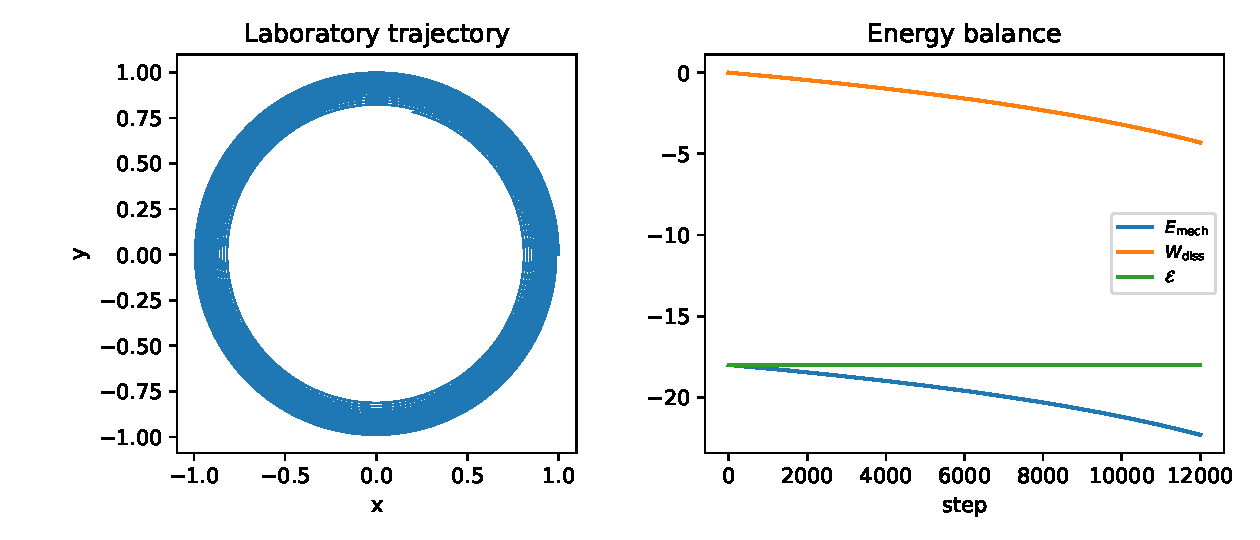
\includegraphics[width=0.92\linewidth]{figs/namcg_gr_simulation_corrected.pdf}
  \caption{Laboratory trajectory and energy balance for
    \eqref{eq:lab-ode} with the toy parameters
    \eqref{eq:toy-params}. The figure is a reduced model.}
  \label{fig:lab}
\end{figure}

If a previously generated PNG from the notes is used instead,
it belongs at this caption and nowhere else in the book.

\section{Code}
\label{sec:ch15-code}

The integrator lives in \texttt{code/namcg\_inspiral.py}. A
minimal version sufficient to produce Figure~\ref{fig:lab} is
the following.

\begin{lstlisting}[style=namcgPythonStyle, caption={Python implementation of the reduced inspiral laboratory velocity-Verlet integrator.}, label={lst:inspiral_code}]
import numpy as np
import matplotlib.pyplot as plt

def run_namcg_laboratory(
    G_toy=36.0,
    eta=0.006,
    M=1.0,
    mu=1.0,
    d0=1.0,
    dt=1.0e-3,
    num_steps=12000,
):
    r = np.array([d0, 0.0])
    v = np.array([0.0, np.sqrt(G_toy * M / d0)])
    traj = np.zeros((num_steps + 1, 2))
    E_mech = np.zeros(num_steps + 1)
    W_diss = np.zeros(num_steps + 1)
    traj[0] = r

    def a_N(r):
        d = np.linalg.norm(r)
        return -G_toy * M * r / d**3

    def a_d(r, v):
        d = np.linalg.norm(r)
        return -eta * v / d**4

    def mechanical_energy(r, v):
        d = np.linalg.norm(r)
        return 0.5 * mu * np.dot(v, v) - G_toy * M * mu / d

    E_mech[0] = mechanical_energy(r, v)
    for n in range(num_steps):
        F_d = mu * a_d(r, v)
        W_diss[n + 1] = W_diss[n] + np.dot(F_d, v) * dt
        v_half = v + 0.5 * dt * (a_N(r) + a_d(r, v))
        r = r + dt * v_half
        v = v_half + 0.5 * dt * (a_N(r) + a_d(r, v_half))
        traj[n + 1] = r
        E_mech[n + 1] = mechanical_energy(r, v)
    return traj, E_mech, W_diss

def plot_laboratory(traj, E_mech, W_diss, filename):
    E_bal = E_mech - W_diss
    fig, axes = plt.subplots(1, 2, figsize=(8.4, 3.6))
    axes[0].plot(traj[:, 0], traj[:, 1], lw=0.8)
    axes[0].set_aspect("equal")
    axes[0].set_xlabel("x")
    axes[0].set_ylabel("y")
    axes[0].set_title("Laboratory trajectory")
    t = np.arange(len(E_mech))
    axes[1].plot(t, E_mech, label=r"$E_{\mathrm{mech}}$")
    axes[1].plot(t, W_diss, label=r"$W_{\mathrm{diss}}$")
    axes[1].plot(t, E_bal, label=r"$\mathcal{E}$")
    axes[1].set_xlabel("step")
    axes[1].set_title("Energy balance")
    axes[1].legend(fontsize=8)
    fig.tight_layout()
    fig.savefig(filename)
    plt.close(fig)

if __name__ == "__main__":
    traj, E_mech, W_diss = run_namcg_laboratory()
    plot_laboratory(
        traj, E_mech, W_diss,
        "figs/namcg_gr_simulation_corrected.pdf",
    )
\end{lstlisting}

Run the file from the project root after creating \texttt{figs/}.
The script writes a vector PDF suitable for the print interior.
A PNG of the same figure, if already produced by an earlier
notebook, may be kept for draft viewing but should not be the
print original.

\section{How to misread the figure, and how not to}
\label{sec:ch15-misread}

The shrinking orbit is not a measurement of \(\eta\) in nature.
The value \(0.006\) was chosen so that decay is visible in
\(1.2\times 10^{4}\) steps. A realistic mutual-information tail
would produce a far smaller \(\eta\) at \(d\gg\ell_A+\ell_B\).

The flatness of \(\mathcal{E}(t)\) is not a proof of
Theorem~\ref{thm:conservation}. It is a check that the laboratory
implements the balance that the theorem requires of any legal
reduction. If \(\mathcal{E}\) is flat and the force law is not
\eqref{eq:Fdiss}, the check has been passed for the wrong theory.

Comparing the laboratory decay time with a LIGO inspiral time is
not a test of NAMCG. The laboratory has no gravitational waves,
no horizons, and no relativity. Section~\ref{sec:ch14-quad}
already stated the regime in which quadrupole losses dominate.

\section{Exercises}
\label{sec:ch15-exercises}

\begin{enumerate}
  \item \textbf{Zero drag.}
    Set \(\eta=0\) and confirm that \(E_{\mathrm{mech}}\) and
    \(|\mathbf{L}|\) are constant at the level of Verlet error.
    What is the size of that error as a function of \(\Delta t\)?
  \item \textbf{Balance.}
    With \(\eta=0.006\), plot \(\mathcal{E}(t)\) for
    \(\Delta t\in\{10^{-3},5\times 10^{-4},2\times 10^{-3}\}\).
    Does the drift shrink with \(\Delta t\)?
  \item \textbf{Illegal drag.}
    Replace \(d^{-4}\) by a constant \(\gamma\) and rerun. Track
    \(W_{\mathrm{diss}}\) as \(d\) decreases. Why is the late
    behaviour a counterexample to Exercise~5 of Chapter~14?
  \item \textbf{Angular momentum.}
    The drag~\eqref{eq:Fdiss} is antiparallel to \(\mathbf{v}\).
    Show that it exerts a torque and compute
    \(\mathrm{d}\mathbf{L}/\mathrm{d}t\). Confirm the identity
    on the numerical trajectory.
  \item \textbf{Units.}
    Restore SI symbols in~\eqref{eq:lab-ode} and assign dimensions
    to \(\eta\). What combination of \(\ell_A,\ell_B,c\) could
    supply those dimensions if \(\eta\) is built from
    \eqref{eq:I-tail}?
\end{enumerate}

\section{Bridge to Chapter~16}
\label{sec:ch15-bridge}

Every extra structure used in applications now has a name:
the regular core~\eqref{eq:f-reg}, the baryon-tracking extra
density of Assumption~\ref{ass:track}, the working drag of
Assumption~\ref{ass:drag}, and the laboratory of this chapter.
Chapter~16 collects the full list of assumptions from
Chapters~3--15, restates the derivation chain of Chapter~1 as a
single page, and writes the observations that would kill the
framework rather than merely constrain \(\eta\).
\chapter[Falsifiers]{Assumptions, Predictions, and Falsifiers}
\label{ch:falsifiers}

\paragraph{Learning outcomes.}
After this chapter the reader should be able to:
\begin{enumerate}
  \item restate the derivation chain of Chapter~1 with the theorem
        numbers now attached;
  \item separate assumptions that kill NAMCG if they fail from
        coefficients that can be adjusted;
  \item name observations that would refute the framework rather
        than merely bound \(\eta\) or \(r_0\);
  \item refuse to treat a successful laboratory plot as evidence
        for Theorems~\ref{thm:mT}--\ref{thm:Leff};
  \item enter Chapter~17 knowing which open calculations are
        optional refinements and which are missing load-bearing
        proofs.
\end{enumerate}

A framework that cannot say what would kill it is not a framework.
This chapter is the scorecard promised in Section~\ref{sec:ch1-checklist}.

\section{The chain, with theorem numbers}
\label{sec:ch16-chain}

The argument of the book is the following sequence, and no shorter
sequence.

\begin{enumerate}
  \item A matrix order parameter \(\Phi^I{}_A\) with potential
        \eqref{eq:V} admits a frame-locking vacuum
        (Assumptions~\ref{ass:frame-lock}, \ref{ass:dictionary}).
  \item A composite vierbein and metric exist in the condensed
        phase (Repair~II,~\eqref{eq:vev-is-frame};
        Definition~\ref{def:composite-metric},
        Assumption~\ref{ass:nondeg}).
  \item Fluctuations split into \(\psi\), \(A_\mu\), \(\omega_{AB}\),
        and \(T_{\mu\nu}\) (Chapter~5).
  \item Entanglement equilibrium on emergent diamonds is a property
        of the condensate vacuum (Assumption~\ref{ass:EE}).
  \item A Fierz--Pauli tensor block is incompatible with that
        equilibrium unless \(m_T=0\) (Theorem~\ref{thm:mT}).
  \item The Euclidean curvature coefficient obeys the conditional,
        truncated heat-kernel identity of Theorem~\ref{thm:Geff};
        physical matching requires specified operators, weights,
        thresholds, continuation, and scheme (Problem~F).
  \item Four-derivative metric operators are EFT vertices, not
        extra poles (Assumption~\ref{ass:EFT-a2}).
  \item Local Lorentz invariance is a gauge symmetry and
        \(\omega_{AB}\) is eaten (Theorem~\ref{thm:locking}).
  \item The conformal mode is heavy (Assumption~\ref{ass:gap-psi}).
  \item The total stress, including \(T_{\mu\nu}^{\mathrm{ent}}\),
        is covariantly conserved (Theorem~\ref{thm:conservation}).
  \item \(\Lambda_{\mathrm{eff}}\) is set by boundary entanglement
        after an ultraviolet subtraction (Theorem~\ref{thm:Leff}).
\end{enumerate}

Items 5, 6, 8, 10, and 11 are theorems \emph{inside} the list of
assumptions that precede them. If an earlier assumption fails, the
later theorem is idle. Phenomenology in Chapters~13--15 sits after
the whole list. It cannot substitute for any line.

\section{Inventory of named assumptions}
\label{sec:ch16-inventory}

The named hypotheses of Parts~II--V are collected here. ``Load-
bearing'' means that failure returns the infrared theory to analog
gravity, scalar-tensor gravity, or an inconsistent extra force.
``Coefficient'' means that failure changes a number or a regime of
validity without destroying the graviton.

\begin{center}
\small
\begin{tabular}{@{}llp{0.38\linewidth}@{}}
\toprule
Tag & Kind & Content \\
\midrule
\ref{ass:aux-metric} & setup & \(g^{(0)}\) is a scaffold \\
\ref{ass:frame-lock} & load-bearing & vacuum
  \(\langle\Phi^I{}_A\rangle=v\delta^I{}_A\) exists \\
\ref{ass:dictionary} & load-bearing & commutator / covariant-derivative
  dictionary \\
\ref{ass:nondeg} & load-bearing & condensed frame is non-degenerate \\
\ref{ass:lorentzian} & load-bearing & signature is Lorentzian \\
\ref{ass:locked-block} & coefficient & extra internal scalars are heavy \\
\ref{ass:EE} & load-bearing & microscopic entanglement equilibrium \\
\ref{ass:gap-psi} & load-bearing & conformal mode is gapped \\
\ref{ass:laplace} & setup & infrared operator is Laplace type \\
\ref{ass:EFT-a2} & load-bearing & \(C^2,R^2\) are vertices, not poles \\
\ref{ass:ECG} & model & cubic truncation in the static spherical
  sector \\
\ref{ass:local-lorentz} & load-bearing & local \(\mathrm{SO}(3,1)\)
  is gauged \\
\ref{ass:Sent-density} & load-bearing & local boundary entropy
  density exists \\
\ref{ass:bdy-EE} & load-bearing & boundary stationarity sets
  \(\Lambda_{\mathrm{eff}}\) \\
\ref{ass:track} & coefficient & static extra density tracks baryons;
  disks use \(\nu_{\sqrt{}}\) of Appendix~\ref{app:empirical} \\
\ref{ass:efe} & coefficient & external field saturates \(\nu\) at \(\nu(g_{\mathrm{ext}})\),
  not \(\nu(g_{\mathrm{N}})\) \\
\ref{ass:drag} & coefficient & working laboratory law
  \(\mathbf{F}_{\mathrm{diss}}\propto -\mathbf{v}/d^4\) \\
\bottomrule
\end{tabular}
\end{center}

Two comments on the table.

First, ``coefficient'' is not a synonym for ``unimportant.''
Assumption~\ref{ass:track} is how galaxies enter the book. If it
fails, galactic claims fail. The graviton claims need not.

Second, Assumption~\ref{ass:dictionary} is the most important
unproved microscopic bridge. If the infrared dictionary from
Presentation~A to Presentation~B cannot be constructed, the heat
kernel of Chapter~8 is a calculation in a different theory than
the matrix action of Chapter~3.

\section{What would kill the framework}
\label{sec:ch16-kill}

The following outcomes are incompatible with NAMCG as written,
not merely with a choice of \(\eta\).

\paragraph{A light extra tensor or a ghost below the cutoff.}
If precision gravity, pulsar timing, or gravitational-wave
propagation requires a second massless or light spin-2 field, or
a ghost pole below \(\LUV\), Theorem~\ref{thm:mT} plus
Assumption~\ref{ass:EFT-a2} has failed.

\paragraph{A light conformal partner.}
If Solar-System or binary-pulsar tests require a Brans--Dicke
parameter that cannot be produced by a heavy \(\psi\), 
Assumption~\ref{ass:gap-psi} has failed and the infrared theory
is scalar-tensor gravity. That is the ceiling of Chapter~1,
reopened.

\paragraph{Non-conservation of the extra stress.}
If an extra acceleration is demanded by data and cannot be written
as \(\nabla^\mu T_{\mu\nu}^{\mathrm{ent}}\) with
Theorem~\ref{thm:conservation} intact---a drag into nowhere, a
preferred-frame force that cannot be improved to a tensor---then
the geometric reading has failed. Analog dissipation remains
possible. Geometrogenesis of the extra channel has not occurred.

\paragraph{Failure of Lorentz locking.}
If the infrared spectrum contains six extra Goldstone polarizations
from \(\omega_{AB}\), Theorem~\ref{thm:locking} has failed. No
later chapter can hide them.

\paragraph{A cutoff that cannot serve Newton and Lorentz together.}
If the only way to obtain \(\Geff=G_{\mathrm{N}}\) forces
\(\LUV\) into a regime where Lorentz-violating \(\Theta^{\mu\nu}\)
corrections are already excluded by current bounds, the
coefficient map and the kinematic algebra cannot coexist.

\paragraph{An induced Einstein--Hilbert term of the wrong sign.}
If a complete heat-kernel evaluation on the locked bundle produces
a repulsive Einstein term that cannot be flipped by fermions or
by the Lorentzian continuation, the infrared force is not gravity.

None of these killers is a rotation curve. None of them is a
pretty laboratory inspiral.

\section{What would only constrain a coefficient}
\label{sec:ch16-constrain}

The following outcomes bound parameters or restrict regimes.
They do not, by themselves, refute Theorems~\ref{thm:mT}--\ref{thm:Leff}.

\begin{itemize}
  \item SPARC ranking of a global \(\nu(g_{\mathrm{N}})\) against
        simple MOND and the published RAR
        (Appendix~\ref{app:empirical}). Frozen
        \(\nu_{\sqrt{}} \) at \(g_\dagger\) is equivalent to the
        RAR and about \(0.2\%\) behind simple MOND in \(\chi^2\);
        baryons-only is not competitive. That is a passed
        coefficient check on disks, not a theorem. A later
        sample that rejects every high-\(g\)-Newtonian,
        low-\(g\)-square-root boost would restrict
        Assumption~\ref{ass:track} to a smaller class of
        systems, or kill the galactic claim only.
  \item Wide binaries in the solar neighbourhood.
        Isolated \(\nu_{\sqrt{}}(g_{\mathrm{N}})\) predicts
        \(\gamma\approx 4\) at \(g_{\mathrm{N}}=10^{-11}\,\mathrm{m\,s^{-2}}\).
        Assumption~\ref{ass:efe} predicts
        \(\gamma\to\nu_{\sqrt{}}(g_{\mathrm{gal}})\approx 1.1\).
        A quality-controlled Gaia sample consistent with Newton
        constrains the isolated reading and is compatible with
        Assumption~\ref{ass:efe}.
        A surviving \(\gamma\approx 1.4\) is not explained by that
        saturation.
        Neither outcome touches Theorems~7.3--12.4.
  \item Cluster lensing or the bullet-cluster mass offset.
        Same status: the extra tensor may fail as a complete
        replacement for particulate dark matter while the graviton
        derivation stands.
  \item Absence of an extra drag in LIGO-band vacuum inspirals.
        Expected if \(\eta\) is negligible at those separations;
        Section~\ref{sec:ch14-quad} already said so.
  \item Absence of a visible core scale \(r_0\) in EHT images or
        ringdowns. Expected if \(r_0\) is microscopic; bounds
        \(\beta_{\mathrm{ECG}}\).
  \item A measured \(\Lambda_{\mathrm{eff}}\) that does not match
        a particular guess for \(S_{\mathrm{ent}}^{\mathrm{(IR)}}\).
        Theorem~\ref{thm:Leff} changes the origin of the scale. It
        does not compute the number.
  \item A different static mutual-information tail does not, by
        itself, determine the drag exponent. The response exponent
        must be calculated from the dynamical force response. The
        \(d^{-4}\) law remains a falsifiable laboratory assumption
        (Assumption~\ref{ass:drag}).
\end{itemize}

\section{Observational checklist}
\label{sec:ch16-obs}

A short list of current and near-term measurements, with the
question each actually asks of the book.

\paragraph{Solar System and pulsar timing.}
Do they tolerate a massive \(\psi\) and a massive torsion at
scale \(v\), and a \(\mu_{\mathrm{ent}}\) that is negligible at
high acceleration? If no, Assumption~\ref{ass:gap-psi} or
\ref{ass:track} dies. If yes, nothing about diamonds has been
tested.

\paragraph{Gravitational waves.}
Is the propagating mode two TT polarizations at the speed of
light, with no extra light tensor? That is a test of
Theorem~\ref{thm:mT} plus Assumption~\ref{ass:EFT-a2}, and it is
already passed at present precision. A measured extra
polarization would be a killer. A measured inspiral-time
deviation at LIGO frequencies is only a bound on \(\eta\).

\paragraph{Black-hole images and ringdowns.}
Is there a visible deviation from Kerr at the photon ring or in
quasi-normal modes? That bounds \(r_0\). A perfectly Kerr object
is compatible with microscopic \(r_0\).

\paragraph{Galaxies, wide binaries, and clusters.}
Do disks accept a single \(\nu_{\sqrt{}}(g_{\mathrm{N}})\) with
\(\nu\to 1\) at Solar-System acceleration?
Appendix~D says yes, at RAR accuracy.
Do solar-neighbourhood wide binaries accept the isolated
evaluation of that law?
No: Assumption~\ref{ass:efe} saturates them at
\(\nu_{\sqrt{}}(g_{\mathrm{gal}})\).
Do merging clusters still require a stress that does not track
baryons?
That remains an open constraint on Assumption~\ref{ass:track}, not on
Theorem~7.3, and the external field is not a substitute for the
lensing offset.

\paragraph{Cosmology.}
Is \(\Lambda_{\mathrm{eff}}\) constant enough for a
Friedmann equation, and is the ultraviolet quartic absent from
the expansion history? This tests Theorem~\ref{thm:Leff} as a
mechanism, not as a number. A detected bulk \(\LUV^4\) vacuum
energy would kill the HBEV subtraction.

\paragraph{Tidal disruptions.}
Is there extra heating or altered fallback that hydrodynamics
plus GR tides cannot account for? A possible window on
Assumption~\ref{ass:drag}. A null result bounds \(\eta\) at
\(r_{\mathrm{t}}\) and nothing else.

\section{Claims the book has not made}
\label{sec:ch16-not-made}

The following sentences do not appear as theorems in this text,
and must not appear on a cover, in an abstract, or in a chapter
heading as if they did.

\begin{itemize}
  \item Dark matter has been explained.
  \item The cosmological-constant problem has been solved
        numerically.
  \item Singularities have been proved absent in dynamical
        collapse.
  \item LIGO inspirals are driven by a \(1/d^4\) drag.
  \item Lorentzian signature has been derived from a Euclidean
        matrix model.
  \item Presentation~A has been reduced to Presentation~B without
        Assumption~\ref{ass:dictionary}.
  \item The rationals \(A,B,C\) in the coefficient map are unique.
  \item Isolated \(\nu_{\sqrt{}}\) has been derived, and wide
    binaries have been predicted without an external field.
\end{itemize}

A sale-ready monograph that prints any of those sentences as
results has left this book and entered advertising.

\section{How to use Chapter~15 in public}
\label{sec:ch16-public}

Figure~\ref{fig:lab} may be shown as a numerical bookkeeping check of
an assumed drag in a Newtonian laboratory. It may not be
shown as ``NAMCG predicting an inspiral.'' The caption must
retain the words ``reduced model.'' The toy value
\(G_{\mathrm{toy}}=36\) must not be silently replaced by
\(G_{\mathrm{N}}\) in a talk slide.

\section{Exercises}
\label{sec:ch16-exercises}

\begin{enumerate}
  \item \textbf{Sort the list.}
    Take any popular article on emergent gravity and assign each
    of its claims to ``killer,'' ``coefficient,'' or ``not a
    claim of this book.''
  \item \textbf{One-page chain.}
    Write the eleven-line chain of Section~\ref{sec:ch16-chain}
    from memory, without looking. Where you stall is the section
    to reread.
  \item \textbf{Design a killer.}
    Propose one measurement, not already listed, that would
    refute Theorem~\ref{thm:mT} without passing through
    \(\eta\). State the null and the fatal outcome.
  \item \textbf{Design a non-killer.}
    Propose one measurement that looks dramatic and would only
    bound \(r_0\).
  \item \textbf{Abstract hygiene.}
    Rewrite a five-sentence abstract of this book that contains
    no sentence from Section~\ref{sec:ch16-not-made}.
\end{enumerate}

\section{Bridge to Chapter~17}
\label{sec:ch16-bridge}

The killers and the coefficients are now distinguished. What
remains is a research agenda: the calculations that would turn
Assumption~\ref{ass:dictionary} into a lemma, recompute
\(A,B,C\), evaluate \(S_{\mathrm{ent}}^{\mathrm{(IR)}}\), derive
\(\mu_{\mathrm{ent}}\) from \(I(A:B)\), including the external-field argument of Assumption~\ref{ass:efe}, and decide whether
Lorentzian signature can be more than Assumption~\ref{ass:lorentzian}.
Chapter~17 writes that agenda at the thickness of a reader who
has read the book and wants to work, not at the thickness of a
grant advertisement.
\chapter[Research agenda]{Open Calculations and a Research Agenda}
\label{ch:agenda}

\paragraph{Learning outcomes.}
After this chapter the reader should be able to:
\begin{enumerate}
  \item distinguish a load-bearing assumption from a critical-path
        problem and an optional refinement;
  \item pick a first calculation that actually moves the framework,
        rather than a calculation that only decorates Chapter~15;
  \item state what would have to be true before NAMCG may be
        described as finished rather than as a programme;
  \item use the appendices as tools, not as a substitute for the
        open problems listed here.
\end{enumerate}

Chapter~16 said what would kill the theory. This chapter says what
would complete it. The two lists are not the same.

\section{What is closed conditionally inside the book}
\label{sec:ch17-closed}

The following are closed \emph{as arguments from named hypotheses
to named conclusions}. They are not closed as derivations from
empty premises.

\begin{itemize}
  \item Composite metric from a non-degenerate condensate frame
        (Repair~II; Definition~\ref{def:composite-metric},
        Assumption~\ref{ass:nondeg}). The Repair~I formula of
        Definition~\ref{def:vierbein} is not a constructed frame
        (Problem~C).
  \item Algebraic split of \(\delta\Phi_{\mu\nu}\) (Chapter~5).
  \item \(m_T=0\) from entanglement equilibrium plus Fierz--Pauli
        (Theorem~\ref{thm:mT}).
  \item The conditional, truncated heat-kernel identity for specified
        sectors and scheme (Theorem~\ref{thm:Geff}); physical
        \(G_{\mathrm{eff}}\) remains open in Problem~F.
  \item Lorentz locking in unitary gauge
        (Theorem~\ref{thm:locking}).
  \item Conservation of the total stress
        (Theorem~\ref{thm:conservation}).
  \item Replacement of a bulk quartic by an infrared boundary
        datum (Theorem~\ref{thm:Leff}).
  \item A legal Newtonian laboratory for
        Assumption~\ref{ass:drag} (Chapter~15).
\end{itemize}

A reader who has worked every exercise through Chapter~16 can
reproduce that list. Reproducing it is not the same as removing
the hypotheses.

\section{Status vocabulary and completion labels}
\label{sec:ch17-labels}

Status words are \emph{OPEN} and \emph{CLOSED CONDITIONALLY}.
Closed conditionally means proved from named hypotheses to named
conclusions; it does not remove those hypotheses. Completion words
are \emph{DERIVED} and \emph{PROGRAMME-CONDITIONAL}. Derived means
that the problem's target has no remaining assumed premise in the
claimed chain. Programme-conditional means an assumption, input,
reduced scope, or unresolved branch remains.

\begin{quote}
Keeping an assumption, treating a quantity as an input, narrowing
the scope, or choosing a scope that leaves a branch unresolved
documents a limitation and keeps the programme conditional. It does
not close the problem or satisfy the finished-derivation criterion
of Section~\ref{sec:ch17-done}. Closure of a critical-path problem
means DERIVED. A reduced-scope result is stated as such and the
problem stays OPEN. A critical-path problem is met for the
matrix-derived label only by a derivation from the matrix theory; an
external justification, model input, imposed premise, or reduced
scope supports at most a scope-limited Presentation-B model.
\end{quote}

OPTIONAL means that a problem may remain open within a stated scope
provided the claim given up is stated. Optional does not mean solved.
Priority words are CRITICAL PATH and OPTIONAL.
In Chapter~16, a \emph{load-bearing assumption} is a premise used by
the chain; it is not thereby a critical-path problem.

\begin{center}
\begin{tabular}{@{}p{0.31\textwidth}p{0.63\textwidth}@{}}
\toprule
Label & Meaning \\
\midrule
\textbf{Completed infrared derivation (matrix-derived)} &
The only label for meeting the five-item criterion in
Section~\ref{sec:ch17-done}; every critical-path problem is DERIVED
for NAMCG from the matrix theory. \\
\textbf{Scope-limited Presentation-B infrared model} &
A separately stated model with its imposed premises named. It is
not matrix-derived, does not close critical-path problems, and does
not satisfy the five-item criterion. \\
\textbf{Programme} &
Any other status; one or more critical-path premises or targets
remain unresolved. \\
\bottomrule
\end{tabular}
\end{center}

\section{Critical-path problems: B, C, and D}
\label{sec:ch17-bearing}

Problems B, C, D, F, and G are critical path for a completed
matrix-derived infrared derivation. The order below follows
dependencies, not project size.

\paragraph{Problem B: entanglement equilibrium from the path
integral.}
\emph{CRITICAL PATH; OPEN.} The fixed-algebra first-law identity
is established, but not the required stationarity.
Assumption~\ref{ass:EE} is the physical engine of
Theorem~\ref{thm:mT}. Derive \(\delta S_D=0\) at fixed volume as
a Ward identity of the microscopic action~\eqref{eq:Smicro}, or
of~\eqref{eq:Smatrix} after Problem~A, without importing Jacobson's
hypothesis from a theory that already has a metric. A replica
computation on small diamonds, with the polar vacuum as background,
is the obvious route. A result that holds only for conformal
fluctuations must be flagged as such, because the tensor block is
not conformal.
Closure requires fixed-volume variations of the tensor (non-conformal)
block from the microscopic action, a specified map
\(g^{(0)}\mapsto g\), and no use of an already-existing metric. A
conformal-only derivation is a sub-case and leaves B OPEN.

\paragraph{Problem C: the conformal mode.}
\emph{CRITICAL PATH; OPEN.} The radial potential curvature is
known, but the physical scalar operator and coupling are not.
Assumption~\ref{ass:gap-psi} is the remaining scalar-tensor
ceiling. Compute the full quadratic scalar operator on the locked
vacuum in a constructed frame: the canonically normalised kinetic
coefficient of the pure-trace scalar (including the induced
Einstein--Hilbert contribution), its mixing with \(T_{\mu\nu}\), its
non-minimal curvature coupling, and its matter coupling. The
potential~\eqref{eq:V} alone fixes only the radial curvature
\(\lambda v^{2}\). From the operator, produce the pole mass, or a
ratio \(m_\psi/v\), together with the coupling that can be compared
with Cassini bounds. If \(m_\psi\) is not parametrically of order
\(\sqrt{\lambda}\,v\), the assumption is false and the infrared
theory must be rewritten as scalar-tensor NAMCG.
Closure requires the operator, scalar coupling, and phenomenological
comparison that define and test either the safe-mass or scalar-tensor
outcome. Declaring a scalar-tensor scope without those data leaves
Problem~C open and the result programme-conditional.

\paragraph{Lemma (tree-level radial mass).}
\label{lem:msigma}
On the locked vacuum \(\langle\Phi^{I}{}_{A}\rangle=v\delta^{I}{}_{A}\),
write the polar field
\(\Phi=(v+\sigma)\Lambda\) with \(\Lambda^{\dagger}\Lambda=\mathbb{I}\)
and \(\langle\sigma\rangle=0\).
Then \(\Phi^{\dagger}\Phi=(v+\sigma)^{2}\mathbb{I}\), and
\eqref{eq:V} collapses to a singlet potential.
With \(N=\mathrm{Tr}(\mathbb{I})\) locked directions,
\begin{equation}
  V
  =\frac{\lambda}{4}N\bigl[(v+\sigma)^{2}-v^{2}\bigr]^{2}
  =N\lambda v^{2}\,\sigma^{2}+O(\sigma^{3}).
\end{equation}
The kinetic term in~\eqref{eq:Smicro}, in the signature \((-,+,+,+)\),
contributes \(-N\,(\partial\sigma)^{2}\).
Canonical normalisation \(\sigma_{c}=\sigma\sqrt{2N}\)
puts the quadratic action in the form
\(-\tfrac12(\partial\sigma_{c})^{2}-\tfrac12 m_{\sigma}^{2}\sigma_{c}^{2}\),
with
\begin{equation}
  \label{eq:msigma}
  m_{\sigma}^{2}=\lambda v^{2},
  \qquad
  m_{\sigma}=v\sqrt{\lambda}.
\end{equation}
The would-be Goldstones in \(\Lambda\) remain massless at this order.
They are the modes Chapter~10 is required to eat.
They are not \(\psi\).

\paragraph{Lemma (radial potential curvature in the pure-trace sector).}
\label{lem:psi-sigma}
Work in the pure-trace sector: \(T_{\mu\nu}=0\), \(F_{\mu\nu}=0\),
and \(\omega_{\mu\nu}=0\). Two repairs of the frame must be
kept distinct.

\emph{Repair II, unitary gauge.}
Chapter~10 permits \(\Lambda=\mathbb{I}\) wherever
Assumption~\ref{ass:nondeg} holds. The vacuum is then the frame,
\(e^{A}{}_{\mu}=\Phi^{A}{}_{\mu}/v\), so
\begin{equation}
  \label{eq:repairII-trace}
  g_{\mu\nu}
  =(1+\sigma/v)^{2}\eta_{\mu\nu},
  \qquad
  \psi
  \equiv\eta^{\mu\nu}h_{\mu\nu}
  =8\sigma/v+O(\sigma^{2}).
\end{equation}
The conformal mode and the radial singlet are the same field in
this gauge. The potential~\eqref{eq:V} gives the radial singlet the
curvature \(V''\propto\lambda v^{2}\), which with the microscopic
kinetic normalisation of Lemma~\ref{lem:msigma} is
\(m_\sigma^{2}=\lambda v^{2}\). This is a statement about the potential
only. It is not yet the mass of a canonically normalised pole of
\(\psi\) (see the identification paragraph below).

\emph{Repair I.}
Definition~\ref{def:vierbein} does not define a vierbein
(Appendix~\ref{app:status}, Section~\ref{sec:status-C}), so \(\psi\)
has no definition in terms of \(\Lambda\) and no Hessian on
\((\sigma,\psi)\) is computed for Repair~I. What survives is that
\eqref{eq:V} depends only on
\(\Phi^{\dagger}\Phi=(v+\sigma)^{2}\mathbb{I}\), so it gives
curvature only to \(\sigma\) and none to the
\(\mathfrak{so}(3,1)\)-valued directions of \(\Lambda\).

\emph{Identification \(g^{(0)}=g[e]\).}
For the metric~\eqref{eq:repairII-trace}, \(g=\Omega^{2}\eta\) with
\(\Omega=1+\sigma/v\), the induced Einstein--Hilbert density is
\(\sqrt{-g}\,R=-6\,\Omega\,\Box\Omega\), which equals
\(6(\partial\Omega)^{2}\) up to a total derivative. With the curvature
convention of Chapter~2, Section~\ref{sec:ch2-manifolds} (identified in
Chapter~9 as the one for which \(R>0\) on spheres), this adds to the
Lagrangian \(+\,3(\partial\sigma)^2/(8\pi G_{\mathrm{eff}}v^{2})\)
if the Einstein--Hilbert term has the form of~\eqref{eq:W-EH} with
\(G_{\mathrm{eff}}>0\); that sign of \(G_{\mathrm{eff}}\) is a declared
condition (Chapter~8, Problem~F), not a derived result. In the signature
\((-,+,+,+)\) a healthy scalar enters as
\(-\tfrac12 Z(\partial\sigma)^2\) with \(Z>0\), so this term has the
conformal-factor (ghost) sign relative to the microscopic term
\(-N(\partial\sigma)^2\) of Lemma~\ref{lem:msigma}. Conditional on the
pure-trace truncation, on adding the induced term to the microscopic one,
and on \(G_{\mathrm{eff}}>0\) in the Lorentzian continuation, the quadratic
action
\(-\tfrac12 Z(\partial\sigma)^2-\tfrac12 V''\sigma^2\) has
\begin{equation}
  \label{eq:Z-sigma}
  Z=2N-\frac{3}{4\pi G_{\mathrm{eff}}v^{2}}
   =2N\Bigl(1-\frac{3M_{\mathrm P}^{2}}{Nv^{2}}\Bigr),
  \qquad
  V''=2N\lambda v^{2},
  \qquad
  M_{\mathrm P}^{2}=\frac1{8\pi G_{\mathrm{eff}}}.
\end{equation}
If \(Nv^{2}>3M_{\mathrm P}^{2}\) then \(Z>0\) and a pole of squared mass
\(m^{2}=V''/Z=\lambda v^{2}\bigl(1-3M_{\mathrm P}^{2}/(Nv^{2})\bigr)^{-1}\)
exists in this truncation; it tends to~\eqref{eq:msigma} only when
\(3M_{\mathrm P}^{2}/(Nv^{2})\to0\), i.e.\
\(G_{\mathrm{eff}}Nv^{2}\to\infty\). For \(Z<0\) (i.e.\
\(Nv^{2}<3M_{\mathrm P}^{2}\)) the truncated mode has a wrong-sign kinetic
term and, with \(\lambda>0\), also \(m^{2}=V''/Z<0\): in this truncation it
is both ghost-like and tachyonic, so the kinetic sign is not the only
instability. The pure-trace truncation therefore cannot support
Assumption~\ref{ass:gap-psi} there; this signals an instability of the
chosen background and truncation and is not a statement about the full
scalar spectrum. At \(Nv^{2}=3M_{\mathrm P}^{2}\) one has \(Z=0\): the
quadratic kinetic term of this truncation degenerates, and the formula
establishes no canonically normalized finite-mass pole there. Since
\(v/M_{\mathrm P}\) requires \(G_{\mathrm{eff}}\), this ties Problem~C to
Problem~F. The mixing with \(T_{\mu\nu}\), the non-minimal curvature
coupling, and the matter coupling are not derived here, and no Cassini
conclusion follows.

\paragraph{Cassini, revised.}
The potential~\eqref{eq:V} gives the radial singlet the curvature
\(\lambda v^{2}\) in the Repair~II pure-trace sector and produces no
massless scalar by itself. The bound
\(\gamma-1=(2.1\pm 2.3)\times 10^{-5}\)
\cite{Bertotti2003}
constrains a massless or long-range scalar partner. Whether the
physical scalar of this sector is short-range on an astronomical
unit depends on the total kinetic coefficient, the non-minimal
coupling and the matter coupling, none of which is computed. This is
not a Cassini bound on NAMCG.

\paragraph{Status of Assumption~\ref{ass:gap-psi}.}
Not promoted. What is established is the potential curvature
\(m_\sigma^{2}=\lambda v^{2}\) (Lemma~\ref{lem:msigma}) and its
identification with the conformal mode in the Repair~II pure-trace
sector, under Assumptions~\ref{ass:frame-lock} and~\ref{ass:nondeg}.
The physical scalar spectrum, the mixing with \(T_{\mu\nu}\) and the
matter coupling remain open (Appendix~\ref{app:status},
Section~\ref{sec:status-C}). Loop corrections and the wrong-sign
conformal kinetic term of the heat kernel remain Chapter~8
bookkeeping.


\paragraph{Problem D: local Lorentz invariance from Presentation~A.}
\emph{CRITICAL PATH; OPEN.} Generator counting is closed
conditionally, while local Lorentz symmetry is imposed.
Assumption~\ref{ass:local-lorentz} puts
\(\mathrm{SO}(3,1)\) into Presentation~B by hand. Either derive a
local Lorentz gauge symmetry from the matrix algebra and condensate
(D1), or state that NAMCG is a theory of a condensate field on an
auxiliary spacetime and stop calling Presentation~A ontologically
prior (D2). D1 closure requires the \(\omega\), \(A_\mu\), \(B\), and
ghost operators and the resulting field content to be specified.
Under D2, even with these operators specified, the result is only a
scope-limited Presentation-B model: D remains OPEN and CRITICAL PATH,
and a full matrix-derived spectrum is not established. The Chapter~10
generator count identifies six
Goldstone orbit variables removable in unitary gauge; it does not
determine the dynamics of the independent diagonal connection \(B\)
or whether torsion vanishes, propagates, or is massive. Torsion-free
\(B\) follows only under the conditional Palatini--Holst hypotheses
of Proposition~\ref{prop:B-torsion-free}; NAMCG has not been shown
to induce them. For a Laplace-type operator,
\(a_1=\operatorname{tr}(R(g)/6-E)\); its explicit universal
curvature term is the Levi-Civita scalar \(R(g)\), while unspecified
\(E\) leaves additional \(B\)-dependence open and does not establish
a Palatini \(R(B)\) term. If \(B\) enters the actual bundle
connection, \(a_2\) may contain \(\operatorname{tr}F(B)^2\); its
survival in the weighted trace depends on unspecified operators and
weights. Deriving the connection and endomorphism dependence or
counting \(B\) and torsion as additional field content remains open;
Problem~D is unresolved.
Within D2, reduced claims may be limited to Levi-Civita metric
geometry of \(g=e^T e\) and conservation of the total stress, without
using \(B\); unitary-gauge Lorentz locking removes the six Goldstone
orbit variables, while frame/metric bookkeeping remains provisional.
D2 does not establish a full-spectrum account, the dynamics or
masslessness of \(B\), torsion-free \(B\), or the quadratic operator
of \(A_\mu\). Problem~F then applies only to an explicitly stated
frame/metric truncation omitting \(B\) and \(A_\mu\), conditional on
that truncation and with the corresponding ghost sector specified.

\section{Open problems by scope and priority}
\label{sec:ch17-coeff}

\subsection{Optional problems A and E}

\paragraph{Problem A: the infrared dictionary.}
\emph{OPEN; OPTIONAL only if Presentation~B is the operative theory
and no claim is made that NAMCG follows from Presentation~A or that
Presentation~A is ontologically prior.} The claim given up is a
derivation from the matrix model; Chapter~8 remains a Presentation-B
calculation. A claim of matrix-model priority makes A critical path.
Assumption~\ref{ass:dictionary} is the map
\begin{equation}
  \label{eq:dict-again}
  [\hat X_\mu,\Phi]
  \;\longleftrightarrow\;
  i\Theta_{\mu\nu}D^\nu\Phi
\end{equation}
plus higher-derivative corrections. A derivation must specify the
Hilbert space, Weyl map, continuum limit, and error at each order in
\(\Theta\).

\paragraph{Problem E: Lorentzian signature.}
\emph{OPEN; OPTIONAL within a scope that retains
Assumption~\ref{ass:lorentzian}.} The claim given up is that
Lorentzian signature is emergent or derived. Euclidean positivity
and a formal Wick rotation do not select it; rotating because the
infrared world is Lorentzian is not a derivation.

\subsection{Critical-path items F and G}

\paragraph{Problem F: the rationals \(A,B,C\).}
\emph{CRITICAL PATH; OPEN.} The conditional heat-kernel identity
does not compute the physical coupling.
The target is to evaluate the weighted \(a_1\) and the
curvature-linear part of \(a_2\) on the locked block, including
diffeomorphism and local-Lorentz ghosts and the radial-mode
threshold, with a scheme stated. The finite-dimensional fibre count
alone does not determine these coefficients: the quadratic operator,
its connection and endomorphism, the determinant weights, and finite
counterterms enter.

\paragraph{Verified heat-kernel bookkeeping (not closure).}
For the proper-time convention of Appendix~\ref{app:seeley-dewitt},
\[
W_E=-\frac12\int_{\LUV^{-2}}^{\mu^{-2}}\frac{\mathrm{d}s}{s}\,
\mathrm{Tr}\,e^{-s\mathcal O},
\]
termwise integration of the truncated, unresummed small-\(s\)
expansion gives the \(a_0,a_1,a_2\) factors
\(-1/(64\pi^2),-1/(32\pi^2),-1/(32\pi^2)\), respectively, with
powers \(\LUV^4-\mu^4\), \(\LUV^2-\mu^2\), and
\(\ln(\LUV^2/\mu^2)\). These are not exact finite-cutoff
integrations of massive determinants; resumming mass exponentials
produces sector-dependent threshold functions. The standard
curvature-square part of \(a_2\) for \(\mathcal O=-D^2+E\) is
\[
\frac1{180}\left(R_{\mu\nu\rho\sigma}R^{\mu\nu\rho\sigma}
-R_{\mu\nu}R^{\mu\nu}+\frac52R^2\right),
\]
not the previously displayed \(7R^2/2\).

For one minimally coupled real bosonic Laplace-type field with
\(E_R=0\), the universal \(a_1\) contribution to the Euclidean
coefficient of \(\int\sqrt{g}\,R_E\) is
\[
C_{R,E}^{(a_1)}
=-\frac{N_0}{192\pi^2}(\LUV^2-\mu^2),
\]
where \(N_0\) is the fibre trace of this single sector and the
displayed limits are assigned to it. For a specified collection,
the corresponding Euclidean contribution is the sum over the
explicitly weighted sectors and their assigned limits. This is not
the full locked-block result and does not establish a ghost-subtracted
trace. It makes no claim about the Lorentzian Einstein--Hilbert sign
or a physical \(G_{\mathrm{eff}}\); those require the specified
sector sum and an explicit action/curvature continuation convention.

If \(E=E_0+QR+\cdots\), the \(a_1\) curvature coefficient is
\(\operatorname{tr}(\tfrac16\mathbb I-Q)\). For a scalar with
\(E=m^2+\xi R\), the mass-dependent curvature-linear term in \(a_2\)
is \((\xi-\tfrac16)m^2R\), vanishing at \(\xi=1/6\). Thus the
conformal radial scalar alone does not establish a nonzero logarithmic
\(B\); the additional frame operator must be specified and evaluated.

\paragraph{Missing step.}
Specify the gauge-fixed quadratic Hessian for every locked-block
field, including bundle connections, endomorphisms, diffeomorphism
and local-Lorentz ghost operators and weights, the radial threshold
prescription, finite counterterms, and continuation convention. Then
compute the weighted \(a_1\) and relevant \(a_2\) terms in that scheme
and match them to \(A,B,C\). The present manuscript does not specify
those data. The asserted net \(+2\) from the on-shell TT count is not
an off-shell heat-kernel trace, and no replacement ghost count can be
inferred without the actual gauge fixing and ghost operators. The
values \(A=1/\pi\), \(B=8\pi/3\), and \(C=0\) are not established.
Problem~F remains open.


\paragraph{Problem G: infrared boundary entropy.}
\emph{CRITICAL PATH; mechanism CLOSED CONDITIONALLY, derivation OPEN.}
Evaluate \(S_{\mathrm{ent}}^{\mathrm{(IR)}}\) on an explicit
cosmological or large-tube boundary and produce a candidate
\(\Lambda_{\mathrm{eff}}\) from~\eqref{eq:Leff}. A symbolic
formula in terms of a late-time entanglement scale is more useful
than a claim to have obtained \(10^{-122}\).

\paragraph{G completion levels.}
For G-model, a scaling or value computed within a stated assumed
boundary model is PROGRAMME-CONDITIONAL and does not satisfy the
matrix-derived completion criterion. For G-external, independently
justified boundary entropy and stationarity may support only a
scope-limited Presentation-B model; G remains open for the
matrix-derived label. G is DERIVED only when the entropy density and
stationarity relation are derived from the matrix theory and
\(\Lambda_{\mathrm{eff}}\) follows from them. A scaling selected to
reproduce a target remains an input. The required entropy density is
the one in Assumption~\ref{ass:Sent-density}, derived by the replica
construction from the matrix theory, and boundary stationarity
Assumption~\ref{ass:bdy-EE} must likewise be derived rather than
retained.

\subsection{Optional problems continued}

\paragraph{Problem H: interpolating function.}
\emph{OPEN; OPTIONAL research within the theory.} The claim given
up is a derivation of \(\nu_{\sqrt{}}\) from modular data; current
empirical comparisons remain coefficient checks.
Derive \(\nu_{\sqrt{}}\) in~\eqref{eq:nu-sqrt}, or a function
that beats it on a SPARC hold-out, from the modular data of
Chapters~6 and~12. The target is
\begin{equation}
  \label{eq:nu-target}
  \nu_{\sqrt{}}(g_{\mathrm{N}})
  =\frac{1}{1-\exp\bigl(-\sqrt{g_{\mathrm{N}}/g_s}\bigr)},
\end{equation}
which is identically \(1+n_{\mathrm{BE}}(\sqrt{g_{\mathrm{N}}/g_s})\).
Appendix~\ref{app:empirical} already shows that this law, frozen
at the published \(g_\dagger\), is equivalent to the RAR and
about \(0.2\%\) behind simple MOND, while baryons-only fails.
That ranking is a coefficient check. It does not solve
Problem~H.

The first finite computation is the replica free energy of a
free field on a weak-field diamond whose infrared boundary is
specified as part of the calculation. Chapter~\ref{ch:hbev} supplies
\(\Lambda_{\mathrm{eff}}\) but does not define a stationary boundary
geometry or its surface gravity \(\kappa_{\mathrm{IR}}\); a
placeholder \(\kappa_{\mathrm{IR}}\) with \(\Lambda=\Lambda_{\mathrm{eff}}\)
must be constructed and normalized there. Read the source-dependent
modular excitation gap \(\Delta k(g_{\mathrm{N}},\kappa_{\mathrm{IR}})\)
when a Newtonian source of acceleration \(g_{\mathrm{N}}\) is introduced;
the absolute lowest eigenvalue is not used, because it depends on an
additive normalization (Section~\ref{sec:status-H}). Problem~H is solved
if the response to the extra stress, computed from the weighted
multimode spectral sum of Section~\ref{sec:status-H} (or from a
justified single-ladder response), reproduces~\eqref{eq:nu-target}
with no SPARC input. In the single-ladder case this requires
\begin{equation}
  \label{eq:gap-H}
  \Delta k
  =
  \sqrt{\frac{g_{\mathrm{N}}}{g_s}},
  \qquad
  g_s=c_\star\,\kappa_{\mathrm{IR}},
\end{equation}
with the order-one constant \(c_\star\) obtained from the calculation
and not from galaxy data. The values \(c_\star=1\) and
\(c_\star=1/(2\pi)\) both appear in this manuscript; neither is
adopted, and a scaling
\(\Delta k\propto\sqrt{g_{\mathrm{N}}/\kappa_{\mathrm{IR}}}\) alone does
not fix \(c_\star\). A computed spectrum that does not reproduce
\eqref{eq:nu-target} does not solve Problem~H. A linear gap
\(\Delta k\propto g_{\mathrm{N}}/\kappa_{\mathrm{IR}}\)
reproduces the retired \(\nu_{\mathrm{exp}}\) and kills
Assumption~\ref{ass:sqrt-mod}.

Alternatively, prove that no local
\(\mu_{\mathrm{ent}}(g_{\mathrm{N}})\) exists and write the
nonlocal kernel instead. Refitting \(\alpha\), \(r_s\), or
\(g_s\) to rotmod files is not a solution. Identifying
\(g_s\) with \(g_\dagger\) inside the replica calculation is
not allowed; compare \(\kappa_{\mathrm{IR}}\) to \(g_\dagger\)
only after the source-dependent gap and response are calculated.

\paragraph{Problem I: dynamical origin of the drag.}
\emph{OPEN; OPTIONAL falsifiable phenomenological extension.}
It becomes critical only if the drag is claimed to be derived or
predicted. Otherwise the microscopic exponent and rate remain open,
and Assumption~\ref{ass:drag} is a working law.
Replace Assumption~\ref{ass:drag} by a low-frequency response
calculation of \(\Gamma_{ij}(\mathbf r;\ell_A,\ell_B)\) from
specified microscopic dynamics and a specified stationary reference
state, including the finite-size factors \(\ell_A,\ell_B\) and the
longitudinal and transverse components. Report the exponent and the
coefficient. Then, and only then, estimate \(\eta\) at
tidal radii and at LIGO-band separations. The static tail and its
assumptions are recorded in Problem~\ref{sec:status-I}; no static-tail
power determines the retarded response.

\paragraph{Problem J: spherical ECG solutions.}
\emph{OPEN; OPTIONAL research within the stated model scope.} The
claim given up is singularity resolution derived from the matrix
theory; reduced results remain conditional on symmetric reduction
and the ECG model assumption.
For the explicit invariant~\(\mathcal P\) in~\eqref{eq:ECG}, used in
the action~\eqref{eq:S-ECG}, Section~\ref{sec:status-J} records
checked reduced Euler--Lagrange
identities, the resulting first integral including
\(\Lambda_{\mathrm{eff}}\), its conditional regular-centre constraint
for every \(\Lambda_{\mathrm{eff}}\), the maximally symmetric
curvature relation, and the large-radius tail. These results are
conditional on the static spherical reduction capturing the full
field equations; that symmetric-criticality step is not established
here. The Einstein-like linearized spectrum on maximally symmetric
backgrounds is cited separately and does not establish nonlinear or
sourced stability. Problem~J remains open: justify the reduction
against the full field equations, establish the cubic truncation and
its microscopic matching, and construct a regular massive core from
specified sourced or modified equations, including its entanglement
stress and residual relative to the phenomenological
profile~\eqref{eq:f-reg}.

\section{Problems that look like work and are not}
\label{sec:ch17-not}

The following activities are useful as exercises and do not move
the framework.

\begin{itemize}
  \item Producing further Newtonian integrators with new colour
        maps of Figure~\ref{fig:lab}.
  \item Fitting SPARC with an unconstrained \(\mu_{\mathrm{ent}}\),
        a per-galaxy \((\alpha,r_s)\), or a new \(\nu\) that is
        not~\eqref{eq:nu-target} and is not derived from
        \(I(A:B)\). Appendix~\ref{app:empirical} already did the
        legitimate coefficient ranking.
  \item Writing \(\mathbf{a}_{\mathrm{irrev}}\) with additional
        free exponents and calling each a prediction.
  \item Replacing \(G_{\mathrm{toy}}\) by \(G_{\mathrm{N}}\) in
        a slide.
  \item Adding adjectives (``holographic,'' ``non-Abelian,''
        ``entropic'') to an abstract without adding a lemma.
\end{itemize}

Chapter~15 exists so that a legal laboratory is on the record.
It does not exist so that the laboratory can become the theory.

\section{A recommended order of work}
\label{sec:ch17-order}

The critical-path dependency order is:

\begin{enumerate}
  \item Problem~D1: derive local \(SO(3,1)\) from the matrix algebra
        and condensate; specify the \(\omega,A_\mu,B\) and ghost
        operators needed by Problem~F.
  \item Problem~C: compute the tree-level scalar operator, including
        kinetic coefficient, mixing, mass and testable matter coupling.
  \item Problem~F: compute \(A,B,C\) with the specified operators,
        ghosts, thresholds and scheme, and derive \(G_{\mathrm{eff}}\).
  \item Problem~B: derive the fixed-volume tensor-block stationarity
        from the microscopic action, not only for conformal variations.
  \item Problem~G: derive \(S_{\mathrm{ent}}^{\mathrm{(IR)}}\) and
        boundary stationarity from the matrix theory, then derive the
        \(\Lambda_{\mathrm{eff}}\) scaling or value.
\end{enumerate}

\paragraph{Alternate scope: model work outside the critical-path sequence.}
Taking Presentation~B with imposed local Lorentz symmetry (D2), an
externally justified boundary result (G-external), or \(G_{\mathrm{eff}}\)
as an input may make a scope-limited Presentation-B model calculable
and testable, for example by specifying full quadratic and ghost
operators and computing Problem~F for a stated truncation. Such work
leaves Problems~D, F, G and the matrix-derived completion criterion
open, must name its imposed premises, and is not a step in the
sequence above.

Problems~A, E, H, I, and J are optional within their stated scopes.
Appendix~\ref{app:empirical} records the coefficient-level check for
Problem~H; further galactic work should not be described as a
derivation from \(I(A:B)\) without the modular calculation.

\section{What ``finished'' would mean}
\label{sec:ch17-done}

The label \emph{Completed infrared derivation (matrix-derived)}
applies only if all five critical-path problems are DERIVED:

\begin{enumerate}
  \item Problem~B is a lemma: Assumption~\ref{ass:EE} is no longer an
        assumption, and fixed-volume variations include the
        non-conformal tensor block.
  \item Problem~C has a computed scalar operator, coupling, and
        phenomenological comparison defining and testing either a
        sufficiently heavy \(m_\psi\) or the scalar-tensor outcome.
  \item Problem~D1: an \(SO(3,1)\) gauge symmetry is derived from the
        matrix algebra and condensate, with the \(\omega,A_\mu,B\)
        and ghost operators specified and the field content stated.
  \item Problem~F has \(A,B,C\) and the sign/scheme dependence of
        \(G_{\mathrm{eff}}\) computed from the specified operators;
        \(G_{\mathrm{eff}}\) is not an input.
  \item Problem~G-derived: the infrared boundary entropy density
        and stationarity relation are derived from the matrix theory,
        and the \(\Lambda_{\mathrm{eff}}\) scaling or value follows
        from them. G-model and G-external do not meet this item.
\end{enumerate}

If local Lorentz symmetry is instead imposed (D2), even with the
full quadratic and ghost content specified, the result is a
scope-limited Presentation-B infrared model. It may be studied and
tested as such, but Problem~D stays OPEN and CRITICAL PATH and the
five-item criterion is not met. No label of ``completed infrared
derivation'' is allowed for that scope. Any critical-path item met
only by an imposed premise, input, or reduced scope likewise yields
at most a scope-limited model or programme, never the matrix-derived
label.

Problems~A, E, H, I, and J may remain open in a completed derivation
within the stated scopes; the claims given up are listed above.
Problem~A is additionally required if the theory is claimed to
follow from Presentation~A. Problem~I is a prerequisite only if
drag is claimed to be derived or predicted.

Until all five items are derived, the honest public description is
the subtitle of the book, read as a programme:
\emph{an attempt} to derive general relativity and massless
spin-2 dynamics from a matrix condensate held at entanglement
equilibrium. The attempt is written so that it can fail in
public. That is the point of Chapter~16.

\section{Exercises}
\label{sec:ch17-exercises}

\begin{enumerate}
  \item \textbf{Status report.}
    Copy the eleven-line chain of Section~\ref{sec:ch16-chain}
    and mark each line ``lemma,'' ``theorem from assumptions,''
    or ``assumption.'' Do not use a mark you cannot defend
    from the text.
  \item \textbf{Proposal.}
    Write a two-page project proposal for Problem~C or Problem~F
    only. Include the first calculation you would perform and
    the result that would make you stop.
  \item \textbf{Not a proposal.}
    Take any project that Section~\ref{sec:ch17-not} would
    reject and explain, in six sentences, why it does not
    change the status of Theorem~\ref{thm:mT}.
  \item \textbf{Public sentence.}
    Write one sentence suitable for an Amazon description that
    survives Section~\ref{sec:ch16-not-made} and the last
    paragraph of Section~\ref{sec:ch17-done}.
\end{enumerate}

\section{Bridge to the appendices}
\label{sec:ch17-bridge}

The main text is complete. Appendix~A records the Seeley--DeWitt
algorithm at the working thickness used in Chapter~8.
Appendix~B records the replica formula and the modular Hamiltonian
at the thickness used in Chapter~6. Appendix~C records the
Verlet laboratory and the energy identity used in Chapter~15.
Appendix~D records the SPARC ranking of \(\nu_{\sqrt{}}\) against
the RAR, simple MOND, and baryons-only. None of the appendices
introduces a new physical hypothesis. If an appendix appears to
do so, the hypothesis belongs in the main text or it does not
belong in the book.

\appendix
\chapter{Seeley--DeWitt Coefficients at Working Thickness}
\label{app:seeley-dewitt}

This appendix records the heat-kernel formulae used in Chapter~8.
It introduces no new physical hypothesis. Conventions follow
Section~\ref{sec:ch2-heatkernel}: Euclidean section first,
Lorentzian continuation afterwards, signature of the main text
restored only when an Einstein--Hilbert term is isolated.

\section{Laplace-type operators}
\label{sec:appA-laplace}

Let \(V\to M\) be a vector bundle over a smooth four-manifold with
Riemannian metric \(g_{\mu\nu}\). A second-order differential
operator on sections of \(V\) is of Laplace type if it can be
written
\begin{equation}
  \label{eq:appA-O}
  \mathcal{O}
  =-g^{\mu\nu}D_\mu D_\nu+E,
\end{equation}
where \(D_\mu=\nabla_\mu+\mathcal{A}_\mu\) is a connection on \(V\)
(including the Levi-Civita connection on tensor factors) and \(E\)
is a bundle endomorphism. The curvature of \(D\) is
\begin{equation}
  \label{eq:appA-F}
  \mathcal{F}_{\mu\nu}
  =[D_\mu,D_\nu].
\end{equation}
On the locked condensate block of Chapter~5, \(V\) is the bundle of
tensors \(\delta\Phi_{\mu\nu}\) together with whatever ghosts are
included in a given computation.

The heat operator \(e^{-s\mathcal{O}}\) is defined for \(s>0\) by
the usual functional calculus after \(\mathcal{O}\) has been made
positive by a Wick rotation. Its integral kernel
\(K(s;x,y)\) satisfies
\begin{equation}
  \label{eq:appA-heat}
  \partial_s K+\mathcal{O}_x K=0,
  \qquad
  K(0;x,y)=\delta(x,y).
\end{equation}

\section{Small-time expansion}
\label{sec:appA-expand}

On the diagonal in four dimensions,
\begin{equation}
  \label{eq:appA-SDW}
  \mathrm{tr}_V K(s;x,x)
  \sim
  \frac{1}{(4\pi s)^{2}}
  \sum_{k=0}^{\infty}
  s^k a_k(x),
  \qquad
  s\to 0^+.
\end{equation}
Each \(a_k\) is a local scalar density of mass dimension \(2k\),
built from \(R_{\mu\nu\rho\sigma}\), \(\mathcal{F}_{\mu\nu}\),
\(E\), and their covariant derivatives. The first three
coefficients, up to total derivatives that do not enter the bulk
effective action, are
\begin{equation}
  \label{eq:appA-a0}
  a_0=\mathrm{tr}_V\mathbb{I},
\end{equation}
\begin{equation}
  \label{eq:appA-a1}
  a_1
  =\mathrm{tr}_V
   \Bigl(
     \tfrac16 R-E
   \Bigr),
\end{equation}
\begin{equation}
  \label{eq:appA-a2}
  \begin{aligned}
    a_2
    =\mathrm{tr}_V
     \Biggl(
       &\frac{1}{180}
        \bigl(
          R_{\mu\nu\rho\sigma}R^{\mu\nu\rho\sigma}
          -R_{\mu\nu}R^{\mu\nu}
          +\tfrac52 R^2
        \bigr)
        +\frac12 E^2
        -\frac16 RE\\
       &+\frac{1}{12}\mathcal{F}_{\mu\nu}\mathcal{F}^{\mu\nu}
        +\frac{1}{30}D^2 R
        -\frac16 D^2 E
     \Biggr).
  \end{aligned}
\end{equation}
Different references redistribute the \(D^2 R\) and \(D^2 E\) terms
by integration by parts. For the bulk action of Chapter~8 those
terms are discarded.

The numerical coefficients in~\eqref{eq:appA-a2} are the standard
DeWitt values for a Laplace-type operator. They do not determine
the coefficients \(A,B,C\) in the conditional
parameterization~\eqref{eq:Geff-structure}. Their evaluation requires
the specified operators, fibre traces, determinant weights, and
thresholds; this remains part of Problem~F in Chapter~17.

\section{Proper-time integrals}
\label{sec:appA-integrals}

For the sectors actually included in a gauge-fixed calculation, let
\(\mathcal{S}_{\mathrm{sec}}\) be their index set, \(w_s\) their determinant weights
relative to a real bosonic determinant, and \(\mathcal O_s\) their
operators. Define
\begin{equation}
  \label{eq:appA-sector-sum}
  W_E^{(1)}
  =\frac12\sum_{s\in\mathcal{S}_{\mathrm{sec}}}w_s
        \operatorname{Tr}_{V_s}\ln\mathcal O_s,
  \qquad
  \mathcal N_0
  :=\sum_{s\in\mathcal{S}_{\mathrm{sec}}}w_s
        \operatorname{tr}_{V_s}\mathbb I_s .
\end{equation}
The corresponding proper-time representation is
\begin{equation}
  \label{eq:appA-W}
  W_E^{(1)}
  =-\frac12\sum_{s\in\mathcal{S}_{\mathrm{sec}}}w_s
    \int_{s_{\min,s}}^{s_{\max,s}}\frac{\mathrm{d}s}{s}\,
    \operatorname{Tr}_{V_s}e^{-s\mathcal O_s}.
\end{equation}
The expressions below are term-by-term integrals of the truncated,
unresummed small-\(s\) heat-kernel expansion through \(a_2\), not
exact finite-cutoff integrations of massive determinants. If \(E_s\)
contains \(m_s^2\), resumming \(\exp(-s m_s^2)\) replaces polynomial
cutoff terms by sector-dependent threshold functions. A common pair of
limits applies only to sectors explicitly assigned those limits;
otherwise the sector-dependent limits are retained. Inserting the
heat-kernel expansion and integrating term by term gives
\begin{equation}
  \label{eq:appA-Wexp}
  \begin{aligned}
      W_E^{(1)}
      &\supset
      \sum_{s\in\mathcal{S}_{\mathrm{sec}}}w_s
      \int\mathrm{d}^4x\,\sqrt{g}\,
      \Biggl[
        -\frac{a_{0,s}}{64\pi^2}
          ({\LUV}_s^4-\mu_s^4)
        -\frac{a_{1,s}}{32\pi^2}
          ({\LUV}_s^2-\mu_s^2)\\
      &\qquad\qquad
        -\frac{a_{2,s}}{32\pi^2}
          \ln\Bigl(\frac{{\LUV}_s^2}{\mu_s^2}\Bigr)
      \Biggr],
  \end{aligned}
\end{equation}
where \(a_{k,s}\) are the traced coefficients on \(V_s\). With common
limits explicitly assigned to every included sector, the \(a_0\) term
is \(-\mathcal N_0(\LUV^4-\mu^4)/(64\pi^2)\).

For the Lorentzian vacuum-sign statement adopt \(S_E=-iS_L\) under
\(t=-i\tau\) and define the Lorentzian vacuum term by
\(S_L\supset-\rho_\Lambda\int\mathrm{d}^4x\,\sqrt{-g}\).
For one real scalar, \(a_0=1\), and only under these conventions,
\(W_E/\mathrm{Vol}\supset-(\LUV^4-\mu^4)/(64\pi^2)\) corresponds to
\(\rho_\Lambda=-(\LUV^4-\mu^4)/(64\pi^2)\). The common-limit sector
sum gives \(\rho_\Lambda=-\mathcal N_0(\LUV^4-\mu^4)/(64\pi^2)\)
only when all displayed sectors share the assigned limits, within the
same truncated, unresummed expansion. The Lorentzian sign is
conditional on this continuation/action convention.

\section{Worked example: a non-minimal scalar}
\label{sec:appA-scalar}

For a single real scalar with
\begin{equation}
  \label{eq:appA-scalar}
  \mathcal{O}=-\nabla^2+\xi R+m^2,
\end{equation}
one has \(E=\xi R+m^2\), \(\mathcal{F}_{\mu\nu}=0\), and
\(\mathrm{tr}_V\mathbb{I}=1\). Then
\begin{equation}
  \label{eq:appA-scalar-a1}
  a_1=\bigl(\tfrac16-\xi\bigr)R-m^2.
\end{equation}
The curvature piece of \(a_1\) cancels at \(\xi=1/6\). That
cancellation removes this scalar's contribution to the curvature
coefficient through \(a_1\). The NAMCG radial
mode is not assumed to sit at \(\xi=1/6\); Exercise~3 of
Chapter~8 is the corresponding warning.

For one real scalar the Euclidean \(a_0\) contribution is
\(-(\LUV^4-\mu^4)/(64\pi^2)\). Under the continuation and Lorentzian
vacuum-action convention stated above, this corresponds to
\(\rho_\Lambda=-(\LUV^4-\mu^4)/(64\pi^2)\). For a collection of
sectors the total density includes their determinant weights and
sector-dependent thresholds.

\section{Fibre traces on the locked block}
\label{sec:appA-fibre}

If \(V\) is the space of symmetric traceless tensors on a
four-manifold, \(\mathrm{tr}_V\mathbb{I}=9\). If the algebraic
split of Chapter~5 is retained before gauge fixing, the sixteen
components of \(\delta\Phi_{\mu\nu}\) give
\(\mathrm{tr}_V\mathbb{I}=16\). Ghosts for diffeomorphisms
contribute with the opposite sign and with their own Laplace-type
operators. Any local-Lorentz ghost sector must be specified together
with the gauge fixing of the independent Lorentz connection;
Theorem~\ref{thm:locking} does not supply that operator.

\(\mathcal N_0\) is the weighted fibre trace over the sectors actually
included, not automatically the locked-block dimension or a
physical-mode count. A total locked-block result must specify the
gauge-fixed fluctuation, Goldstone, diffeomorphism-ghost and
local-Lorentz-ghost operators, determinant weights, and assigned
thresholds. No factor of \(1/6\) is absorbed into \(\mathcal N_0\);
the complete calculation is Problem~F.

\section{What this appendix will not do}
\label{sec:appA-not}

It will not list \(a_3\) and \(a_4\). Those coefficients generate
six- and eight-derivative operators that the book treats as
suppressed by further powers of \(\LUV^{-1}\).

It will not prove the coefficients~\eqref{eq:appA-a0}--\eqref{eq:appA-a2}.
Standard derivations (coincidence limits of the Synge world
function, or the recursive DeWitt transport equations) are in the
references collected in \texttt{bib/namcg.bib}. The book uses the
coefficients; it does not redo the recursion.

It will not evaluate \(a_2\) on the Einsteinian cubic background
of Chapter~13. That evaluation is part of Problem~J if it is
needed, not part of the working thickness of Chapter~8.

\section{Exercises}
\label{sec:appA-exercises}

\begin{enumerate}
  \item \textbf{Dimensions.}
    Assign mass dimensions to \(s\), \(a_0\), \(a_1\), \(a_2\),
    and \(\mathrm{tr}_V K(s;x,x)\). Confirm that each term in
    \eqref{eq:appA-Wexp} has dimension four.
  \item \textbf{Conformal scalar.}
    Set \(\xi=1/6\) and \(m=0\) in~\eqref{eq:appA-scalar-a1}.
    What remains of \(a_1\)? What remains of the \(\LUV^2 R\)
    term in \(W_E\)?
  \item \textbf{Gauss--Bonnet combination.}
    Rewrite the curvature part of~\eqref{eq:appA-a2} in the
    basis \(\{C_{\mu\nu\rho\sigma}C^{\mu\nu\rho\sigma},R^2,
    E_{\mathrm{GB}}\}\). Which combination multiplies a
    topological density in four dimensions?
  \item \textbf{Ghost sign.}
    A diffeomorphism ghost in the background-field gauge is a
    complex vector with a Laplace-type operator. What factor
    multiplies its contribution to \(a_0\) relative to a real
    scalar, and why is the sign opposite to a physical field?
  \item \textbf{Conditional curvature coefficient.}
    Given specified sector operators, determinant weights, proper-time
    limits, and a finite-counterterm scheme, derive the truncated
    Euclidean curvature coefficient from \(a_1\) and \(a_2\). Identify
    the additional data needed for its Lorentzian continuation and
    comparison with \(G_{\mathrm{eff}}\).
\end{enumerate}
\chapter{Modular Hamiltonians and the Replica Formula}
\label{app:modular}

This appendix records the entanglement formulae used in
Chapters~6, 11, and~12. It introduces no new physical hypothesis.
The working identity of the main text remains
Proposition~\ref{prop:ward}. What follows is the language in which
that identity was written.

\section{States, reductions, and von Neumann entropy}
\label{sec:appB-vN}

Let \(\mathcal{H}\) be the Hilbert space of the microscopic theory
and \(\rho\) a density operator on \(\mathcal{H}\). For a von
Neumann algebra \(\mathcal{A}_D\) of observables associated with a
region \(D\), the reduced state \(\rho_D\) is the restriction of
\(\rho\) to \(\mathcal{A}_D\). In a tensor-product approximation
\(\mathcal{H}\simeq\mathcal{H}_D\otimes\mathcal{H}_{D^c}\),
\begin{equation}
  \label{eq:appB-rhoD}
  \rho_D=\mathrm{Tr}_{\mathcal{H}_{D^c}}\rho.
\end{equation}
Continuum quantum field theory does not have that tensor-product
factorization. The algebraic definition (restriction to
\(\mathcal{A}_D\)) is the honest one; equation~\eqref{eq:appB-rhoD}
is the formula used in every explicit replica computation in the
book.

The von Neumann entropy and modular Hamiltonian of \(\rho_D\) are
\begin{equation}
  \label{eq:appB-SH}
  S_D=-\mathrm{Tr}(\rho_D\ln\rho_D),
  \qquad
  H_D=-\ln\rho_D,
\end{equation}
so that
\begin{equation}
  \label{eq:appB-S-eq-H}
  S_D=\langle H_D\rangle_{\rho_D}.
\end{equation}
If \(\rho_D\) has kernel, \(\ln\rho_D\) is defined on the support
of \(\rho_D\) and \(S_D\) may be infinite. In quantum field theory
\(S_D\) is ultraviolet divergent. Differences \(\delta S_D\) at
fixed cutoff, and mutual informations, are the finite objects used
in the main text.

\section{Relative entropy and mutual information}
\label{sec:appB-rel}

For two states \(\rho\) and \(\sigma\) on the same algebra,
\begin{equation}
  \label{eq:appB-rel}
  S(\rho\|\sigma)
  =\mathrm{Tr}(\rho\ln\rho)-\mathrm{Tr}(\rho\ln\sigma)
\end{equation}
is non-negative and vanishes if and only if \(\rho=\sigma\)
(when the expression is finite). Mutual information of two
regions \(A\) and \(B\) is the relative entropy of \(\rho_{AB}\)
with respect to \(\rho_A\otimes\rho_B\),
\begin{equation}
  \label{eq:appB-MI}
  I(A:B)
  =S(\rho_{AB}\|\rho_A\otimes\rho_B)
  =S(A)+S(B)-S(A\cup B),
\end{equation}
the second equality holding when the three von Neumann entropies
are regulated in the same scheme. Positivity of \(I(A:B)\) is
therefore positivity of relative entropy. That is the source of
the sign in Definition~\ref{def:Uent} and of
\(\Gamma(d)\ge 0\) in Chapter~14.

Strong subadditivity,
\begin{equation}
  \label{eq:appB-SSA}
  S(A\cup B)+S(B\cup C)
  \ge S(B)+S(A\cup B\cup C),
\end{equation}
is recorded for completeness. The main text does not use it
beyond the positivity of \(I(A:B)\).

\section{The replica formula}
\label{sec:appB-replica}

For integer \(n\ge 1\),
\begin{equation}
  \label{eq:appB-replica}
  \mathrm{Tr}\,(\rho_D)^n
  =Z_n/Z_1^n,
\end{equation}
where \(Z_n\) is the partition function of the microscopic theory
on an \(n\)-sheeted cover branched over the edge
\(\mathcal{B}=\partial D\cap\Sigma\). Analytic continuation in
\(n\) and the identity
\begin{equation}
  \label{eq:appB-replica-S}
  S_D
  =\lim_{n\to 1}
   \bigl(1-n\partial_n\bigr)\ln\mathrm{Tr}\,(\rho_D)^n
\end{equation}
produce the von Neumann entropy. Differentiating at \(n=1\)
inserts a single modular Hamiltonian: the first variation
\(\delta S_D=\delta\langle H_D\rangle\) used in Chapter~6 is the
replica formula at first order, not a second definition.

In Presentation~B the cover is a branched cover of the auxiliary
manifold, later identified with the emergent spacetime by
Proposition~\ref{prop:scaffold}. In Presentation~A the same
construction requires Problem~A of Chapter~17.

\section{Bisognano--Wichmann and small diamonds}
\label{sec:appB-BW}

On Minkowski space, let \(W\) be a Rindler wedge. The
Bisognano--Wichmann theorem identifies the modular Hamiltonian of
the vacuum restricted to \(W\) with the boost generator that
fixes the edge,
\begin{equation}
  \label{eq:appB-BW}
  H_W
  =\frac{2\pi}{\kappa}
   \int_{\Sigma\cap W}
   \mathrm{d}\Sigma^\mu\,\xi^\nu T_{\mu\nu},
\end{equation}
where \(\xi^\mu\) is the boost Killing vector and
\(\kappa\) its surface gravity (equal to \(1\) in standard Rindler
coordinates, restored here for matching~\eqref{eq:HD-boost}).

A small causal diamond in a slowly curved emergent geometry is,
to leading order in Riemann normal coordinates~\eqref{eq:RNC}, a
compact analogue of two opposing Rindler wedges glued at a
2-sphere. The working formula~\eqref{eq:HD-boost} is that analogue:
the same boost-energy integral plus an area term
\(H_{\mathrm{area}}\) whose first variation is
\(\delta A/(4\Geff)\) after Chapter~8 has named \(\Geff\). The
error is \(O(\ell^3)\) in the diamond radius, which is the order
dropped in Proposition~\ref{prop:ward}.

The identification is exact for free fields in Rindler space. It
is an operator-product approximation for interacting condensate
fluctuations. The book does not claim a Bisognano--Wichmann
theorem for the full matrix potential~\eqref{eq:V}.

\section{Fixed volume}
\label{sec:appB-volume}

Jacobson's entanglement-equilibrium condition is imposed at fixed
spatial volume of the maximal slice. In Riemann normal coordinates
the volume of a small ball of radius \(\ell\) is~\eqref{eq:vol-exp}.
A pure conformal variation \(\delta g_{\mu\nu}=\chi\eta_{\mu\nu}\)
changes that volume at order \(\ell^3\). Holding \(V\) fixed
removes that breathing from the comparison and is why the conformal
block \(\psi\) and the tensor block \(T_{\mu\nu}\) do not enter
the first law on the same footing.

Fixed volume is a constraint on the variations admitted in
Assumption~\ref{ass:EE}. It is not a statement that \(\psi\) is
massive. That statement is Assumption~\ref{ass:gap-psi}.

\section{Boundary entropy versus diamond entropy}
\label{sec:appB-two}

Chapter~12 uses a different functional: a local density
\(S_{\mathrm{ent}}(h_{ij},\phi)\) on \(\partial M\). The replica
construction of that density is the same formula,
\eqref{eq:appB-replica-S}, applied to a thin tubular neighbourhood
of the boundary and then localized as in
Assumption~\ref{ass:Sent-density}. The two functionals must not be
substituted for each other. Section~\ref{sec:ch12-diamonds}
already assigned them different jobs.

\section{What this appendix will not do}
\label{sec:appB-not}

It will not develop Tomita--Takesaki theory beyond the definition
\(H_D=-\ln\rho_D\). It will not compute \(S_D\) for the matrix
potential~\eqref{eq:V}. It will not prove Assumption~\ref{ass:EE}.
Those are Problem~B of Chapter~17 and the physical input of
Chapter~6, respectively.

\section{Exercises}
\label{sec:appB-exercises}

\begin{enumerate}
  \item \textbf{Replica derivative.}
    From~\eqref{eq:appB-replica-S} and
    \(\mathrm{Tr}\,\rho^n=\exp(\ln\mathrm{Tr}\,\rho^n)\), recover
    \(S=\langle H\rangle\) at \(n=1\).
  \item \textbf{Relative entropy and Klein's inequality.}
    For finite-dimensional density matrices, prove
    \(S(\rho\|\sigma)\ge 0\). Deduce \(I(A:B)\ge 0\).
  \item \textbf{Rindler temperature.}
    In standard Rindler coordinates, show that the Unruh
    temperature seen by an accelerated observer is
    \(\kappa/2\pi\). Match the factor in~\eqref{eq:appB-BW}.
  \item \textbf{Area divergence.}
    For a free scalar in Minkowski space, the unregulated
    \(S_D\) diverges as \(\mathrm{Area}(\mathcal{B})/\epsilon^2\).
    Why do mutual information and first variations \(\delta S_D\)
    at fixed cutoff remain useful?
  \item \textbf{Two functionals.}
    Write four sentences explaining why a small-diamond \(S_D\)
    cannot be used as the boundary density of Definition~\ref{def:HBEV}.
\end{enumerate}
\chapter{Verlet Laboratory and Energy Identity}
\label{app:integrator}

This appendix records the integrator and the energy identity used
in Chapter~15. It introduces no new physical hypothesis. The force
law is Assumption~\ref{ass:drag}. The bookkeeping reference is
Proposition~\ref{prop:allowed-drag}, which this laboratory does not
satisfy in the microscopic sense; the integrator tracks only
\(W_{\mathrm{diss}}\). The source file is
\texttt{code/namcg\_inspiral.py}.

\section{Reduced equation}
\label{sec:appC-ode}

In the reduced-mass frame the laboratory system is
\begin{equation}
  \label{eq:appC-ode}
  \ddot{\mathbf{r}}
  =\mathbf{a}_{\mathrm{N}}(\mathbf{r})
   +\mathbf{a}_{\mathrm{d}}(\mathbf{r},\mathbf{v}),
\end{equation}
with
\begin{equation}
  \label{eq:appC-acc}
  \mathbf{a}_{\mathrm{N}}
  =-\frac{G_{\mathrm{toy}}M}{d^{3}}\mathbf{r},
  \qquad
  \mathbf{a}_{\mathrm{d}}
  =-\frac{\eta}{d^{4}}\mathbf{v},
  \qquad
  d=|\mathbf{r}|.
\end{equation}
The conservative force is Newtonian. The drag is
\eqref{eq:Fdiss} with \(\mu\) cancelled. Toy parameters are
\eqref{eq:toy-params}.

\section{One step}
\label{sec:appC-step}

Let \(\Delta t>0\). Given \((\mathbf{r}_n,\mathbf{v}_n)\),
\begin{equation}
  \label{eq:appC-verlet}
  \begin{aligned}
    \mathbf{v}_{1/2}
    &=\mathbf{v}_n
      +\tfrac12\Delta t
       \bigl(
         \mathbf{a}_{\mathrm{N}}(\mathbf{r}_n)
         +\mathbf{a}_{\mathrm{d}}(\mathbf{r}_n,\mathbf{v}_n)
       \bigr),\\
    \mathbf{r}_{n+1}
    &=\mathbf{r}_n+\Delta t\,\mathbf{v}_{1/2},\\
    \mathbf{v}_{n+1}
    &=\mathbf{v}_{1/2}
      +\tfrac12\Delta t
       \bigl(
         \mathbf{a}_{\mathrm{N}}(\mathbf{r}_{n+1})
         +\mathbf{a}_{\mathrm{d}}(\mathbf{r}_{n+1},\mathbf{v}_{1/2})
       \bigr).
  \end{aligned}
\end{equation}
When \(\eta=0\) this is velocity Verlet for a position-dependent
force and is second-order accurate and symplectic on the
conservative phase space. When \(\eta\neq 0\) the last drag
evaluation uses \(\mathbf{v}_{1/2}\) rather than
\(\mathbf{v}_{n+1}\), so the dissipative piece is explicit and
the scheme is no longer symplectic. The local error in the drag
kick remains \(O(\Delta t^{2})\).

An implicit alternative replaces
\(\mathbf{a}_{\mathrm{d}}(\mathbf{r}_{n+1},\mathbf{v}_{1/2})\)
by \(\mathbf{a}_{\mathrm{d}}(\mathbf{r}_{n+1},\mathbf{v}_{n+1})\)
and solves a linear equation for \(\mathbf{v}_{n+1}\). The
published script does not do that. The difference is visible only
if one drives \(\Delta t\) up to the orbital period.

\section{Mechanical energy, work, and balance}
\label{sec:appC-energy}

Define
\begin{equation}
  \label{eq:appC-E}
  E_{\mathrm{mech}}
  =\frac12\mu v^{2}-\frac{G_{\mathrm{toy}}M\mu}{d}
\end{equation}
and the accumulated work
\begin{equation}
  \label{eq:appC-W}
  W_{\mathrm{diss}}(t_{n+1})
  =W_{\mathrm{diss}}(t_n)
   +\mathbf{F}_{\mathrm{diss}}(\mathbf{r}_n,\mathbf{v}_n)
    \cdot\mathbf{v}_n\,\Delta t,
\end{equation}
with \(\mathbf{F}_{\mathrm{diss}}=\mu\mathbf{a}_{\mathrm{d}}\) and
\(W_{\mathrm{diss}}(0)=0\). Along exact solutions of
\eqref{eq:appC-ode},
\begin{equation}
  \label{eq:appC-identity}
  \frac{\mathrm{d}E_{\mathrm{mech}}}{\mathrm{d}t}
  =\mathbf{F}_{\mathrm{diss}}\cdot\mathbf{v},
\end{equation}
because the Newtonian force is minus the gradient of
\(U_{\mathrm{N}}=-\Geff\)-less toy potential
\(-G_{\mathrm{toy}}M\mu/d\). Therefore
\begin{equation}
  \label{eq:appC-bal}
  \mathcal{E}(t)
  \equiv
  E_{\mathrm{mech}}(t)-W_{\mathrm{diss}}(t)
\end{equation}
is constant on exact solutions. On discrete solutions it is
constant up to the quadrature error in~\eqref{eq:appC-W} and the
Verlet error in~\eqref{eq:appC-verlet}. A systematic drift that
does not shrink with \(\Delta t\) means the implementation does
not obey~\eqref{eq:appC-identity} and is illegal in the sense of
Section~\ref{sec:ch14-legal}.

A trapezoidal quadrature,
\begin{equation}
  \label{eq:appC-trap}
  \Delta W
  =\frac12
   \Bigl(
     \mathbf{F}_{\mathrm{diss},n}\cdot\mathbf{v}_n
     +\mathbf{F}_{\mathrm{diss},n+1}\cdot\mathbf{v}_{n+1}
   \Bigr)\Delta t,
\end{equation}
reduces that drift by one order in \(\Delta t\). The published
script uses the left-endpoint rule~\eqref{eq:appC-W} because it
is enough to make \(\mathcal{E}\) look flat on the scale of
Figure~\ref{fig:lab}.

\section{Angular momentum}
\label{sec:appC-L}

The Newtonian force is central and exerts no torque. The drag is
antiparallel to \(\mathbf{v}\), so
\begin{equation}
  \label{eq:appC-torque}
  \frac{\mathrm{d}\mathbf{L}}{\mathrm{d}t}
  =\mathbf{r}\times\mathbf{F}_{\mathrm{diss}}
  =-\eta\mu\frac{\mathbf{r}\times\mathbf{v}}{d^{4}}.
\end{equation}
Angular momentum is therefore not conserved when \(\eta\neq 0\).
That is required: an inspiral that conserved \(|\mathbf{L}|\) at
fixed mass would be incompatible with a shrinking circular orbit.
The identity~\eqref{eq:appC-torque} is a useful code check
(Exercise~4 of Chapter~15).

\section{Initial data and units}
\label{sec:appC-ic}

The published run uses
\begin{equation}
  \label{eq:appC-ic}
  \mathbf{r}(0)=(1,0),\qquad
  \mathbf{v}(0)=(0,\sqrt{G_{\mathrm{toy}}M}),
\end{equation}
with \(G_{\mathrm{toy}}=36\), \(\eta=0.006\), \(\Delta t=10^{-3}\),
and \(1.2\times 10^{4}\) steps. These are code units. They are
chosen so that decay is visible, not so that \(\eta\) matches a
tidal-disruption estimate from Problem~I of Chapter~17.

Restoring dimensions, \(\eta\) in~\eqref{eq:appC-acc} has dimension
\(\mathrm{length}^{4}/\mathrm{time}\), since
\(\mathbf{a}=-\eta\mathbf{v}/d^{4}\). The static tail
\eqref{eq:I-tail} does not supply this coefficient; deriving it
requires the response calculation of Problem~\ref{sec:status-I},
which this appendix does not attempt.

\section{How to run the script}
\label{sec:appC-run}

From the project root, after \texttt{figs/} exists:
\begin{verbatim}
python code/namcg_inspiral.py
\end{verbatim}
The script writes
\texttt{figs/namcg\_gr\_simulation\_corrected.pdf}. Point
Figure~\ref{fig:lab} at that PDF for the print interior. A
legacy PNG from an earlier notebook may be kept for draft
viewing.

If \texttt{matplotlib} is unavailable, the integrator still runs
and can write \texttt{traj}, \texttt{E\_mech}, and
\texttt{W\_diss} to text; the figure is then optional.

\section{What this appendix will not do}
\label{sec:appC-not}

It will not introduce gravitational waves, horizons, or a
relativistic two-body Hamiltonian. It will not treat
\(G_{\mathrm{toy}}\) as \(G_{\mathrm{N}}\). It will not fit
\(\eta\) to data. Those refusals are the content of
Sections~\ref{sec:ch15-misread} and~\ref{sec:ch16-public}.

\section{Exercises}
\label{sec:appC-exercises}

\begin{enumerate}
  \item \textbf{Conservative order.}
    With \(\eta=0\), measure the secular drift of
    \(E_{\mathrm{mech}}\) over \(10^{4}\) steps at three values
    of \(\Delta t\). Confirm second-order scaling.
  \item \textbf{Quadrature.}
    Replace~\eqref{eq:appC-W} by~\eqref{eq:appC-trap} and compare
    the drift of \(\mathcal{E}\).
  \item \textbf{Implicit drag.}
    Solve the linear equation for \(\mathbf{v}_{n+1}\) when the
    last drag evaluation uses \(\mathbf{v}_{n+1}\). Does
    \(\mathcal{E}\) improve enough to justify the extra algebra?
  \item \textbf{Torque check.}
    Integrate~\eqref{eq:appC-torque} in lockstep with the
    trajectory and compare with \(\mathbf{L}_{n+1}-\mathbf{L}_n\).
  \item \textbf{Illegal control.}
    Set \(\mathbf{a}_{\mathrm{d}}=-\gamma\mathbf{v}\) with
    constant \(\gamma\) and watch \(W_{\mathrm{diss}}\) as
    \(d\) decreases. This is Exercise~3 of Chapter~15, recorded
    here so the appendix can be used alone as a lab sheet.
\end{enumerate}
\chapter{SPARC Rotation Curves: A Coefficient-Level Consistency Check}
\label{app:empirical}

\section{What is being tested}
\label{sec:sparc-what}

The function
\begin{equation}
  \label{eq:appD-nu}
  \nu_{\sqrt{}}(g_{\mathrm{N}},g_s)
  =\frac{1}{1-\exp\bigl(-\sqrt{g_{\mathrm{N}}/g_s}\bigr)}
\end{equation}
is the published Radial Acceleration Relation interpolator of
McGaugh, Lelli \& Schombert (2016). Appendix~\ref{app:status}
records that a derivation of this (or any other) interpolator from
the mutual-information functional remains open (Problem~H). The
present appendix asks only whether the same function, with the
single scale fixed at the published value
\(g_s=g_\dagger=1.20\times10^{-10}\,\mathrm{m\,s^{-2}}\),
is compatible with the SPARC rotation-curve sample.

The predicted circular velocity is
\begin{equation}
  \label{eq:appD-V}
  V=V_{\mathrm{b}}\sqrt{\nu_{\sqrt{}}(g_{\mathrm{N}},g_s)},
\end{equation}
where \(V_{\mathrm{b}}\) is the Newtonian baryonic contribution
computed from the SPARC mass models. No additional galactic
parameters are introduced.

\section{SPARC comparison}
\label{sec:sparc-comparison}

The comparison uses the public SPARC rotmod files
(175 galaxies, 3391 radial points). Three models are scored by
\(\chi^2\) and AIC:

\begin{itemize}
  \item baryons only (\(\nu=1\));
  \item simple MOND with one free acceleration scale \(a_0\);
  \item \(\nu_{\sqrt{}}\) with \(g_s\) fixed at \(g_\dagger\)
        (zero free parameters) and, for reference, with \(g_s\) free.
\end{itemize}

\begin{table}[htbp]
\centering
\caption{Global \(\chi^2\) and AIC on 175 SPARC galaxies (3391 points).
Lower AIC is better.}
\label{tab:sparc_results}
\begin{tabular}{lrrrr}
\toprule
Model & Free params & \(\chi^2\) & AIC & Scale (\(\mathrm{m\,s^{-2}}\)) \\
\midrule
\(\nu_{\sqrt{}}\) (fixed \(g_s=g_\dagger\)) & 0 & \(1.695\times10^5\) & \(1.695\times10^5\) & \(1.20\times10^{-10}\) \\
\(\nu_{\sqrt{}}\) (free \(g_s\))            & 1 & \(1.695\times10^5\) & \(1.695\times10^5\) & \(1.20\times10^{-10}\) \\
Simple MOND (free \(a_0\))                 & 1 & \(1.691\times10^5\) & \(1.691\times10^5\) & \(1.16\times10^{-10}\) \\
Baryons only                               & 0 & \(1.960\times10^6\) & \(1.960\times10^6\) & --- \\
\bottomrule
\end{tabular}
\end{table}

The fixed-\(g_s\) and free-\(g_s\) versions of \(\nu_{\sqrt{}}\) are
statistically indistinguishable; the free fit returns
\(g_s=1.20\times10^{-10}\,\mathrm{m\,s^{-2}}\). Relative to the
best one-parameter MOND fit the \(\chi^2\) penalty is
approximately \(0.2\%\). Both modified-gravity models improve on
baryons-only by more than an order of magnitude in \(\chi^2\).

\section{Numerical implementation}
\label{sec:sparc-code}

\begin{lstlisting}[style=namcgPythonStyle,caption={Core evaluation functions.}]
import numpy as np

KMS2_PER_KPC_TO_SI = 1.0e6 / 3.085677581491367e19
G_DAGGER = 1.20e-10

def gn_si(vb, r):
    r = np.maximum(np.asarray(r, float), 1e-6)
    return (np.asarray(vb, float)**2 / r) * KMS2_PER_KPC_TO_SI

def nu_sqrt(gn, gs):
    gs = max(float(gs), 1e-18)
    x = np.clip(np.asarray(gn, float)/gs, 0.0, 1e12)
    s = np.sqrt(x)
    denom = 1.0 - np.exp(-s)
    nu = np.empty_like(denom)
    tiny = denom < 1e-12
    nu[tiny] = 1.0 / np.maximum(s[tiny], 1e-30)
    nu[~tiny] = 1.0 / denom[~tiny]
    return nu

def v_namcg(r, vb, gs=G_DAGGER):
    return vb * np.sqrt(np.clip(nu_sqrt(gn_si(vb, r), gs), 1.0, 1e6))
\end{lstlisting}

\section{What the comparison is and is not}
\label{sec:sparc-status}

At low Newtonian acceleration,
\(\nu_{\sqrt{}}\) approaches the square-root map
\(g_{\mathrm{obs}}\approx\sqrt{g_{\mathrm{N}}g_\dagger}\).
On the SPARC disks this keeps \(V\) from falling as fast as
\(V_{\mathrm{b}}\). The numerical result shows that this
particular function, frozen at the published \(g_\dagger\),
is compatible with the sample at the same level as a
one-parameter MOND fit.

The comparison does not:
\begin{itemize}
  \item derive \(\nu_{\sqrt{}}\) from \(I(A:B)\) or from the
        modular spectrum (Problem~H remains open);
  \item fix \(g_\dagger\) from the condensate;
  \item constrain \(m_T=0\), the heat-kernel coefficients, or
        the conservation identity;
  \item rule out particle dark-matter halos on other scales.
\end{itemize}

It is a coefficient-level consistency check: the infrared
equation of the monograph can wear the published RAR
interpolator without contradiction on this data set. That is
the strongest statement the SPARC sample supports.
\chapter{A Provisional Bridge from Mutual Information to the RAR}
\label{app:rar-bridge}

This appendix states the strongest logical contact between NAMCG
and the SPARC radial acceleration relation that the book can
currently defend. It does not solve Problem~H. It does not
derive \(g_\dagger\) from \(\Phi^I{}_A\). It replaces an
unspecified \(\mu_{\mathrm{ent}}\) with a single modular
conjecture whose failure would leave Appendix~\ref{app:empirical}
as a coefficient ranking and nothing more.

\section{What the two sides already share}
\label{sec:appE-share}

NAMCG, after Theorems~\ref{thm:mT}--\ref{thm:conservation}, is
Einstein gravity plus a conserved extra tensor obtained by
varying an entanglement functional of baryonic regions. In a
static disk that statement has three immediate consequences,
none of which uses SPARC.

\begin{enumerate}
  \item The extra acceleration is slaved to the baryonic
        Newtonian field. It cannot be an independent halo
        function of \(r\) (Assumption~\ref{ass:track}).
  \item At Solar-System and inner-disk accelerations the extra
        piece must vanish, or Cassini bounds fail:
        \(\nu\to 1\) as \(g_{\mathrm{N}}\to\infty\).
  \item The only scalar available to mark the transition is an
        acceleration built from the same modular data that
        defined the diamonds of Chapter~6 and the infrared
        boundary of Chapter~12.
\end{enumerate}

A fourth consequence is needed once the subsystem is not isolated.
The entanglement functional is a functional of the baryonic
configuration, not of an excised disk. A slowly varying external
Newtonian field \(\mathbf{g}_{\mathrm{ext}}\) therefore enters the
argument of the boost (Assumption~\ref{ass:efe}). In the
external-field-dominated limit \(g_{\mathrm{N}}\ll g_{\mathrm{ext}}\),
\begin{equation}
  \label{eq:appE-efe}
  \gamma
  \equiv\frac{g_{\mathrm{int}}}{g_{\mathrm{N}}}
  \to\nu_{\sqrt{}}(g_{\mathrm{ext}}),
\end{equation}
not \(\nu_{\sqrt{}}(g_{\mathrm{N}})\).
At the Sun, \(v_{\odot}^{2}/R_{0}\approx 2.2\times 10^{-10}\,\mathrm{m\,s^{-2}}
\approx 1.8\,g_{\dagger}\), so \(\nu_{\sqrt{}}(g_{\mathrm{gal}})\approx 1.1\).
An isolated evaluation of~\eqref{eq:appE-RAR} at
\(g_{\mathrm{N}}=10^{-11}\,\mathrm{m\,s^{-2}}\) wants \(\gamma\approx 4\)
and is illegal for a solar-neighborhood binary.

The RAR is an empirical map of exactly that type
\cite{McGaugh2016,Lelli2017RAR}:
\begin{equation}
  \label{eq:appE-RAR}
  g_{\mathrm{obs}}
  =\nu_{\mathrm{RAR}}(x)\,g_{\mathrm{N}},
  \qquad
  x=\frac{g_{\mathrm{N}}}{g_\dagger},
  \qquad
  \nu_{\mathrm{RAR}}(x)
  =\frac{1}{1-e^{-\sqrt{x}}},
\end{equation}
with \(g_\dagger=(1.20\pm 0.02)\times 10^{-10}\,\mathrm{m\,s^{-2}}\)
and residuals that do not track radius or Hubble type. Appendix~\ref{app:empirical}
showed that~\eqref{eq:appE-RAR}, frozen at \(g_\dagger\), is the
disk law NAMCG is presently allowed to wear.

The shared content is therefore the \emph{logical type} of the
law, not the algebra of the interpolator and not the numerical
value of \(g_\dagger\).

\section{Why the first NAMCG-shaped interpolator failed}
\label{sec:appE-failed}

Chapter~6 records the large-separation scaling
\begin{equation}
  \label{eq:appE-I}
  I(A:B)
  \;\sim\;
  c_{p_*}
  \left(\frac{\ell_A\ell_B}{d^2}\right)^{p_*},
  \qquad d\gg\ell_A,\ell_B,
\end{equation}
with \(p_*\) and \(c_{p_*}\) defined as in
Eq.~\eqref{eq:I-falloff}: \(p_*\) is the smallest sum of scaling
dimensions of operators whose product has vacuum quantum numbers.
Cardy~\cite{Cardy2013MI} obtains this form for the R\'enyi mutual
information of compact regions in a conformal vacuum, with the von
Neumann limit shown explicitly for free-scalar spheres; its use for
NAMCG cores is an assumption. The first NAMCG-shaped interpolator
nevertheless converted a gradient of this static tail into a local
boost, producing the working family
\begin{equation}
  \label{eq:appE-exp}
  \nu_{\mathrm{exp}}
  =\frac{1}{1-\alpha\exp(-g_{\mathrm{N}}/g_s)}.
\end{equation}
That conversion is not derived: a static separation gradient is not
a retarded response or a local acceleration interpolator.
On the same 175 SPARC files that family lost to simple MOND by a
wide AIC gap. The transition was too sharp in \(g_{\mathrm{N}}\)
and needed a second amplitude \(\alpha\) that disks do not want.

The failure is useful. It shows that ``mutual information
implies a boost'' is not enough. The \emph{argument of the
exponential} matters. SPARC selects \(\sqrt{g_{\mathrm{N}}}\)
in that argument, not \(g_{\mathrm{N}}\).

\section{An algebraic identity, not a derivation}
\label{sec:appE-BE}

Write \(y=\sqrt{x}=\sqrt{g_{\mathrm{N}}/g_\dagger}\). Then
\begin{equation}
  \label{eq:appE-BE}
  \nu_{\mathrm{RAR}}(x)
  =1+\frac{1}{e^{y}-1}
  =1+n_{\mathrm{BE}}(y),
\end{equation}
where \(n_{\mathrm{BE}}\) is the Bose--Einstein occupation of a
single mode with dimensionless energy \(y\). This is an identity.
It does not, by itself, mean that galactic baryons are a Bose
gas. It does mean that any microscopic argument that produces a
thermal factor \(e^{-\sqrt{g_{\mathrm{N}}/g_s}}\) in a
screen occupation, rather than \(e^{-g_{\mathrm{N}}/g_s}\),
lands on the published interpolator automatically.

The linear-exponential~\eqref{eq:appE-exp} is the Boltzmann
factor of a scale set by \(g_{\mathrm{N}}\) itself. The RAR is
the Bose factor of a scale set by \(\sqrt{g_{\mathrm{N}}}\).
That is the whole algebraic distinction.

\section{A modular conjecture}
\label{sec:appE-conj}

Chapter~6 already assigns a diamond an Unruh temperature
\(T_{\mathrm{Unruh}}=\kappa/2\pi\) and a modular Hamiltonian
\(H_D\). Chapter~12 already assigns the cosmology an infrared
boundary scale through \(\Lambda_{\mathrm{eff}}\). Milgrom's
coincidence~\cite{Milgrom1983},
\begin{equation}
  \label{eq:appE-coinc}
  2\pi g_\dagger
  \;\sim\;
  cH_0
  \;\sim\;
  c^2\sqrt{\Lambda/3},
\end{equation}
says that the SPARC scale sits, to a factor of order \(2\pi\),
on the same infrared accelerations NAMCG already possesses as
diamond and boundary data.

\begin{assumption}[Square-root modular response]
  \label{ass:sqrt-mod}
  For a slowly varying disk of condensed parcels, the
  leading reversible variation of \(U_{\mathrm{ent}}\) with
  respect to a local Newtonian acceleration is thermal in
  the variable
  \begin{equation}
    \label{eq:appE-y}
    y
    =\sqrt{\frac{g_{\mathrm{N}}}{g_s}},
    \qquad
    g_s
    \sim
    \frac{\kappa_{\mathrm{IR}}}{2\pi},
  \end{equation}
  where \(\kappa_{\mathrm{IR}}\) is the surface gravity of the
  infrared boundary used in Chapter~12, not a new galactic
  parameter. The occupation that weights the extra stress is
  \(n_{\mathrm{BE}}(y)\). Then
  \(\nu=1+n_{\mathrm{BE}}(y)\) is~\eqref{eq:appE-RAR}, and
  \(g_s\) is identified with \(g_\dagger\) rather than fitted
  to SPARC.
\end{assumption}

Assumption~\ref{ass:sqrt-mod} is the missing sentence of
Problem~H. It is not implied by Theorem~\ref{thm:mT}. It is
not implied by the conformal tail~\eqref{eq:appE-I}. It is
the simplest contact that turns the book's modular objects
into the interpolator SPARC already selected.

Why a square root rather than a linear Unruh factor
\(T\propto g_{\mathrm{N}}\) is not derived here. A linear
factor reproduces~\eqref{eq:appE-exp} and has already failed.
A justification would have to come from the spectrum of
\(H_D\) on a diamond whose size is set by the local
baryonic curvature radius, or from a two-horizon sharing
between the local diamond and the HBEV boundary. That
calculation is the content of Problem~H, restated.

\section{What this bridge excludes}
\label{sec:appE-exclude}

Verlinde's 2016 emergent-gravity formula for finite disks
depends explicitly on radius as well as on \(g_{\mathrm{N}}\).
Lelli, McGaugh and Schombert found that those residuals
correlate with radius and that acceptable fits require
stellar mass-to-light ratios in tension with population
synthesis~\cite{Lelli2017Verlinde}. NAMCG cannot take that
route. Assumption~\ref{ass:track} plus the RAR residuals
already require a map of \(g_{\mathrm{N}}\) only.

A cosmological running \(g_s(z)\propto H(z)\) is likewise
not licensed by this appendix. Equation~\eqref{eq:appE-coinc}
is a present-day coincidence used to name \(g_s\). Promoting
it to \(g_s(z)\) is extra physics and would have to survive
high-redshift rotation curves before it is written as a
NAMCG result.

Isolated application of~\eqref{eq:appE-RAR} to wide binaries is
likewise not licensed. Assumption~\ref{ass:efe} saturates the boost at
\(\nu_{\sqrt{}}(g_{\mathrm{ext}})\). A Gaia sample consistent with
Newton constrains the isolated reading, not Theorem~7.3.
A reported \(\gamma\approx 1.4\) that survives quality cuts is not
explained by \(\nu_{\sqrt{}}(g_{\mathrm{gal}})\approx 1.1\); that
residual, if real, is still open.

\section{How the bridge would be confirmed or killed}
\label{sec:appE-test}

\paragraph{Confirmation.}
The published diamond first law recovers Einstein gravity
at first order in the metric, hence \(\nu\to 1\).
An interpolator requires the modular spectrum of \(K_D\)
in the two-scale geometry of Chapters~6 and~12
(local diamond plus infrared surface gravity
\(\kappa_{\mathrm{IR}}\)).
Problem~H is solved if the leading eigenvalue for a
weak-field source is
\(\lambda_0\propto\sqrt{g_{\mathrm{N}}/\kappa_{\mathrm{IR}}}\)
and the occupation is bosonic. Then
\(g_s=\kappa_{\mathrm{IR}}\) is not a SPARC fit, and
Appendix~\ref{app:empirical} becomes a consistency check.
A linear eigenvalue
\(\lambda_0\propto g_{\mathrm{N}}/\kappa_{\mathrm{IR}}\)
would reproduce the retired
\(\nu_{\mathrm{exp}}\) and kill
Assumption~\ref{ass:sqrt-mod}.

The same computation must grow an external-field argument
before wide binaries are a prediction. Until it does,
Assumption~\ref{ass:efe} is a coefficient in the same sense as
Assumption~\ref{ass:track}: it is the QUMOND external-field limit written
with \(\nu_{\sqrt{}}\), not a lemma from \(I(A:B)\).

The explicit modular Hamiltonian of de~Sitter diamonds
\cite{Frob2023dS} is the operator to use for the
eigenvalue test~\eqref{eq:lambda0}.
The Euclidean Schwarzschild--de~Sitter action is minus
the sum of the two horizon entropies, not a geometric
mean of surface gravities; that instanton does not
by itself produce \(\sqrt{g_{\mathrm{N}}/\kappa_{\mathrm{IR}}}\).
The numerical coincidence
\(cH_0/2\pi\sim g_\dagger\) may be recorded after
\(\lambda_0\) is computed, not used to fix \(g_s\).

\paragraph{Failure.}
The same computation produces~\eqref{eq:appE-exp}, a
radius-dependent kernel, or a light \(\psi\). Then disks
may still follow the RAR, but not as a NAMCG prediction.
Assumption~\ref{ass:track} remains a coefficient; Problem~H
remains open; Appendix~\ref{app:empirical} is unchanged.

\section{One paragraph for Chapter~13}
\label{sec:appE-ch13}

The working disk law is~\eqref{eq:appE-RAR}.
The reason NAMCG is allowed to use it on an isolated disk is
Assumption~\ref{ass:track}.
The reason a subsystem embedded in the Galaxy must not use the
isolated evaluation is Assumption~\ref{ass:efe}.
The reason the book might eventually own either sentence is
Assumption~E.1.
Until the last is a lemma, the first two are borrowed, and the
galactic sector is the RAR with the external-field effect.

\section{Exercises}
\label{sec:appE-ex}

\begin{enumerate}
  \item Prove~\eqref{eq:appE-BE} in three lines.
  \item Expand \(\nu_{\mathrm{RAR}}\) and \(\nu_{\mathrm{exp}}\)
        for \(x\ll 1\) and \(x\gg 1\). Where do they first
        differ by order one?
  \item Using \(H_0=70\,\mathrm{km\,s^{-1}\,Mpc^{-1}}\), compute
        \(cH_0\) and \(cH_0/2\pi\) in \(\mathrm{m\,s^{-2}}\).
        Compare with \(g_\dagger\). This is a coincidence
        check, not a derivation.
  \item Why does an explicit \(r\) in \(\nu\), as in Verlinde's
        finite-disk formula, threaten the residual structure
        reported by~\cite{Lelli2017RAR}?
  \item \textbf{External field.}
    Take \(g_{\mathrm{ext}}=2.2\times 10^{-10}\,\mathrm{m\,s^{-2}}\)
    and \(g_{\mathrm{N}}=10^{-11}\,\mathrm{m\,s^{-2}}\).
    Compute \(\nu_{\sqrt{}}(g_{\mathrm{N}})\) and
    \(\nu_{\sqrt{}}(g_{\mathrm{ext}})\).
    Which one is the legal boost under Assumption~\ref{ass:efe}, and which
    published wide-binary claim does each contact?
\end{enumerate}
\chapter{Einstein Gravity Plus a Conserved Extra Tensor}
\label{app:field-eq}

This appendix writes the infrared field equation of
Theorems~\ref{thm:mT}--\ref{thm:conservation} next to
Einstein's equation. It introduces no new hypothesis.

\section{Einstein}
\begin{equation}
  \label{eq:appF-Ein}
  G_{\mu\nu}+\Lambda g_{\mu\nu}
  =8\pi G\,T_{\mu\nu}^{\mathrm{matter}}.
\end{equation}
Bianchi identities force
\(\nabla^\mu T_{\mu\nu}^{\mathrm{matter}}=0\) on shell.

\section{NAMCG infrared equation}
After the composite metric, \(m_T=0\), the heat-kernel map,
Lorentz locking, and conservation are granted,
\begin{equation}
  \label{eq:appF-NAMCG}
  G_{\mu\nu}+\Lambda_{\mathrm{eff}}g_{\mu\nu}
  =8\pi\Geff
  \bigl(
    T_{\mu\nu}^{\mathrm{matter}}
   +T_{\mu\nu}^{\mathrm{tensor}}
   +T_{\mu\nu}^{\mathrm{ent}}
  \bigr).
\end{equation}
\(G_{\mu\nu}\) is the Einstein tensor of the composite metric
\(g_{\mu\nu}=\eta_{AB}e^A{}_\mu e^B{}_\nu\).
\(\Lambda_{\mathrm{eff}}\) is the coefficient of
Theorem~\ref{thm:Leff}; \(G_{\mathrm{eff}}\) is to be matched by the
conditional sector calculation of Problem~F.
The extra source is
\begin{equation}
  \label{eq:appF-Tent}
  T_{\mu\nu}^{\mathrm{ent}}
  =-\frac{2}{\sqrt{-g}}
   \frac{\delta U_{\mathrm{ent}}[I(A:B)]}{\delta g^{\mu\nu}}
  =T_{\mu\nu}^{\mathrm{ent,rev}}
   +T_{\mu\nu}^{\mathrm{ent,irrev}}.
\end{equation}
Chapter~11 requires
\begin{equation}
  \label{eq:appF-cons}
  \nabla^\mu
  \bigl(
    T_{\mu\nu}^{\mathrm{matter}}
   +T_{\mu\nu}^{\mathrm{tensor}}
   +T_{\mu\nu}^{\mathrm{ent}}
  \bigr)
  =0.
\end{equation}
In the infrared, \(T_{\mu\nu}^{\mathrm{tensor}}\) is absorbed
into the Einstein tensor of \(g_{\mu\nu}\). What can appear
as extra gravity in static disks is
\(T_{\mu\nu}^{\mathrm{ent,rev}}\).

\section{Weak field}
Newtonian gauge, static source:
\begin{equation}
  \label{eq:appF-Poisson}
  \nabla^2\Phi
  =4\pi\Geff
   \bigl(\rho_{\mathrm{b}}+\rho_{\mathrm{ent}}\bigr),
  \qquad
  \rho_{\mathrm{ent}}
  =T_{00}^{\mathrm{ent,rev}}.
\end{equation}
Assumption~\ref{ass:track} slaved \(\rho_{\mathrm{ent}}\) to
\(\rho_{\mathrm{b}}\). The interpolator \(\nu_{\sqrt{}}\) of
Appendix~\ref{app:empirical} is a coefficient choice for that
assumption, not a consequence of~\eqref{eq:appF-NAMCG}.

\section{What this does and does not change}
High acceleration:
\(T_{\mu\nu}^{\mathrm{ent,rev}}\to 0\), so~\eqref{eq:appF-NAMCG}
returns to~\eqref{eq:appF-Ein} with
\((\Geff,\Lambda_{\mathrm{eff}})\) in place of \((G,\Lambda)\).
Low acceleration: \(\rho_{\mathrm{ent}}\) may dominate
\(\rho_{\mathrm{b}}\) without a particle halo, if and only if
Assumption~\ref{ass:track} holds.
Clusters, the CMB, and colliding systems test that assumption,
not \(G_{\mu\nu}\).
Gravitational waves test \(m_T=0\), not~\eqref{eq:appF-Tent}.
The irreversible drag of Chapter~14 is a phenomenological addition,
not a static extra potential and not derived from
\eqref{eq:appF-Tent}.

\section{One-line summary}
Einstein equates curvature to ordinary stress. NAMCG equates
the same curvature to ordinary stress plus a divergenceless
entanglement stress of baryonic regions.
\chapter{Heat-Kernel Area Term on a Causal Diamond}
\label{app:matrix_entropy}

This appendix records the standard heat-kernel contribution to the
entanglement entropy of a causal diamond. It does not derive the
equilibrium condition \(\delta S_D=\delta\langle H_D\rangle\) and does
not recover the Einstein equation from the matrix sector alone.

\section{Replica formula and cone expansion}
\label{sec:replica-cone}

The von Neumann entropy of the reduced state on a diamond \(D\) is
obtained from the replica trick,
\begin{equation}
  S_D=\bigl(1-n\partial_n\bigr)\ln Z(n)\Big|_{n=1},
\end{equation}
where \(Z(n)\) is the partition function on the \(n\)-sheeted cover
branched along the entangling surface \(\Sigma\). For a Laplace-type
fluctuation operator the heat-kernel expansion on the cone produces
the area term
\begin{equation}
  S_D=\frac{\operatorname{Area}(\Sigma)}{4G_{\mathrm{eff}}}+S_{\mathrm{pot}},
\end{equation}
with the prefactor identified from the Seeley--DeWitt coefficient
that multiplies the deficit. This is the standard result used in
Chapter~6 and Appendix~B. The numerical value of \(G_{\mathrm{eff}}\)
remains the structural heat-kernel map of Theorem~\ref{thm:Geff};
the coefficients \(A,B,C\) are not fixed here (Problem~F).

\section{What is not derived}
\label{sec:not-derived}

\begin{itemize}
  \item The equilibrium condition
        \(\delta S_D=\delta\langle H_D\rangle\) under fixed volume.
        It is the hypothesis of Chapters~6--7 that forces \(m_T=0\).
        It is not obtained as a path-integral Ward identity from the
        replica variation alone.
  \item An evaluation of the fluctuation operator of the locked
        NAMCG condensate (including diffeomorphism and local-Lorentz
        ghosts) that would determine the precise endomorphism
        contribution to the area coefficient.
  \item Recovery of the infrared equation. Once the area law and the
        equilibrium condition are both assumed, the Einstein equation
        with a matrix source follows by the usual Jacobson argument;
        that assumption is not removed.
\end{itemize}

\section{Status}
\label{sec:status}

The area term in \(S_D\) is the standard heat-kernel result. The
appendix adds no new derivation of the Ward identity, no scheme-fixed
coefficient, and no alteration to the open-problem ledger of
Appendix~\ref{app:status}.
\chapter{Status of the Open Problems}
\label{app:status}

This appendix records the precise status of Problems A--J as of the present text.
It collects standard supporting calculations that are already rigorous, states
the exact missing step for each problem, and does not convert any open problem
into a lemma. The research agenda of Chapter~\ref{ch:agenda} remains the
authoritative list; this appendix is a working ledger.

\section{Problem A: matrix-to-modular map}
\label{sec:status-A}

The Weyl--Wigner expansion
\begin{equation}
  [\hat{X}_\mu,\hat{\Phi}]
  =i\Theta_{\mu\nu}D^\nu\Phi
  +\frac{1}{24}\Theta_{\mu\alpha}\Theta_{\beta\gamma}D^\alpha D^\beta D^\gamma\Phi
  +\mathcal{O}(\Theta^3)
\end{equation}
is a standard result of the Moyal product (see the infrared dictionary
discussion in Section~\ref{sec:ch3-relate}). This expansion relates the matrix commutator to a continuum
derivative, but it does not provide the required map from
\((\hat X,\Phi)\) to the causal-diamond modular Hamiltonian \(H_D\)
or the mutual-information functional \(U_{\mathrm{ent}}[I(A:B)]\)
before the composite metric is defined.

\paragraph{Missing step.}
An error-controlled map from the matrix order parameter (or from
\([\hat{X},\Phi]\)) into the modular Hamiltonian \(H_D\) of a causal diamond,
or into the mutual-information functional \(U_{\mathrm{ent}}[I(A:B)]\),
that holds before the composite metric is defined. Until that map is a lemma,
Chapter~8 computes a heat kernel in a theory whose relation to Chapter~3 is
still Assumption~\ref{ass:dictionary}.

\section{Problem B: replica Ward identity}
\label{sec:status-B}

For a differentiable family of normalized reduced states on a fixed
diamond algebra, the first variation of the entropy obeys the standard
first-law identity
\[
\delta S_D
=
\operatorname{Tr}(\delta\rho_D H_D^{(0)})
=
\delta\langle H_D^{(0)}\rangle,
\qquad
H_D^{(0)}=-\ln\rho_D^{(0)},
\]
where the modular Hamiltonian is held fixed at the reference state.
Under the usual path-integral assumptions, the replica construction
expresses this variation as a response of the microscopic action
insertion on the branched cover. These identities do not imply
\(\delta S_D=0\).

\paragraph{Missing step.}
Derive from the microscopic dynamics the entanglement-stationarity
condition \(\delta S_D=0\) for the allowed fixed-volume variations,
and establish the area contribution and its relation to the
\emph{emergent} metric without presupposing that metric or the
fluctuation split of Chapter~5. For variations of the auxiliary
scaffold, the replica insertion computes a response to
\(g^{(0)}_{\mu\nu}\); relating it to the emergent metric still
requires a specified map between them. Problem~B therefore remains
open, although the fixed-algebra first-law identity is established.

\section{Problem C: conformal mode and Cassini}
\label{sec:status-C}

The radial singlet has the tree-level mass
\[
m_\sigma^2=\lambda v^2.
\]
This does not by itself determine the mass or matter coupling of a
scalar mode of the composite metric. In particular, the stated
Repair~I prescription is intended to build a vierbein from the Lorentz-valued
polar factor \(\Lambda\), evaluated at \(\sigma=0\), rather than from
the radial field.

\paragraph{Obstruction to the stated Repair I frame.}
Suppose \(\Lambda(x)\in\mathrm{SO}(3,1)\) and expand about the locked
configuration,
\[
\Lambda=\mathbb I+\Omega+O(\Omega^2),
\qquad
\Omega_{\mu\nu}=-\Omega_{\nu\mu}.
\]
Then \(\partial_\mu\Omega_{\alpha\beta}\) transforms in
\(V\otimes\mathfrak{so}(3,1)\), where \(V=(\tfrac12,\tfrac12)\)
is the Lorentz vector representation. After complexification,
\[
\bigl(V\otimes\mathfrak{so}(3,1)\bigr)_{\mathbb C}
=
\left(\tfrac32,\tfrac12\right)
\oplus\left(\tfrac12,\tfrac12\right)
\oplus\left(\tfrac12,\tfrac32\right)
\oplus\left(\tfrac12,\tfrac12\right).
\]
A vierbein fluctuation transforms in \(V\otimes V\), whose
complexified decomposition is
\[
(V\otimes V)_{\mathbb C}
=
(0,0)\oplus(1,0)\oplus(0,1)\oplus(1,1).
\]
These representations have no common irreducible summand. Hence
there is no nonzero Lorentz-equivariant linear map from
\(\partial_\mu\Omega_{\alpha\beta}\) to a vierbein fluctuation using
only the locked Lorentz-invariant tensors. Consistently, the displayed
formula
\[
e^A{}_\mu=\left\langle\partial_\mu\Lambda^A{}_I\right\rangle
\]
leaves \(I\) uncontracted and does not, as written, define a vierbein.

A simple proposed contraction with a fixed nonzero internal vector
\(n^I\) does not repair non-degeneracy. If
\[
e^A{}_\mu=\partial_\mu\Lambda^A{}_I\,n^I,
\]
then Lorentz orthogonality gives
\[
(\Lambda n)_A e^A{}_\mu
=
(\Lambda n)_A\partial_\mu(\Lambda n)^A
=
\frac12\partial_\mu\bigl((\Lambda n)^2\bigr)
=0.
\]
Every column of \(e^A{}_\mu\) therefore lies in the
three-dimensional subspace orthogonal to \(\Lambda n\), so
\(\operatorname{rank}(e)\leq 3\). This contraction cannot produce a
non-degenerate four-dimensional frame.

\paragraph{Status.}
Under the stated Repair~I ingredients, the linearized composite
vierbein required for the later metric-scalar analysis is not
constructed. This is an obstruction to that frame prescription, not
a proof that a completed theory has or lacks a physical scalar pole.
Repair~II, an independent coframe, or additional symmetry-breaking
background tensors would change the construction and require a
separate analysis. The radial mass \(m_\sigma^2=\lambda v^2\) remains
established, but it is not a metric-scalar mass. The scalar spectrum
and matter coupling relevant to Cassini are therefore still
undetermined. The Repair~II pure-trace relation \(\psi=8\sigma/v\)
with \(m_\sigma^2=\lambda v^2\) is a potential-only statement; the
induced Einstein--Hilbert term adds to the kinetic coefficient of
\(\sigma\), so it does not fix a physical pole mass, mixing or
Cassini coupling.

\section{Problem D: local Lorentz}
\label{sec:status-D}

The counting of generators under the locked vacuum is given in
Chapter~10. The condensate term supplies a quadratic Higgs-type
contribution in the broken-direction combination \(\Xi\); it does not
establish a physical pole mass without kinetic terms and canonical
normalization. The diagonal connection's dynamics and torsion remain
open. Torsion-free behavior follows only under the conditional
Palatini--Holst hypotheses of Proposition~
\ref{prop:B-torsion-free}; NAMCG has not been shown to induce those
hypotheses.

For a Laplace-type operator,
\(a_1=\operatorname{tr}(R(g)/6-E)\); the explicit universal
curvature term is the Levi-Civita scalar \(R(g)\). Because \(E\) is
unspecified, no conclusion about additional \(B\)-dependence of
\(a_1\) follows, and a Palatini \(R(B)\) term is not established. If
\(B\) enters the bundle connection of the actual operator, \(a_2\)
may contain a \(\operatorname{tr}F(B)^2\) term; whether it survives
in the weighted trace depends on the unspecified operator
representation and weights. Deriving the \(B\)-dependence of \(E\)
and the bundle connection remains open.

\paragraph{Missing step.}
Derive \(\mathrm{SO}(3,1)\) from the matrix algebra alone, or state
that Presentation~A is not ontologically prior (the present text
does the latter), and derive the effective dynamics of the
independent diagonal connection or retain it as unresolved field
content. Generator counting alone does not settle its torsion or
propagating modes.

\section{Problem E: signature}
\label{sec:status-E}

Euclidean positivity of the matrix action and the formal Wick rotation of
one coordinate are recorded. They do not select Lorentzian signature without
an additional hypothesis.

\paragraph{Status.}
Remains Assumption~\ref{ass:lorentzian}.

\section{Problem F: coefficients \(A,B,C\)}
\label{sec:status-F}

The conditional, truncated heat-kernel identity is
Theorem~\ref{thm:Geff}; it is not a computed \(A,B,C\)
parameterization or physical value of \(G_{\mathrm{eff}}\).

\paragraph{Missing step.}
Specify the gauge-fixed fluctuation, Goldstone, diffeomorphism-ghost,
and local-Lorentz-ghost operators and weights; per-sector proper-time
limits; massive threshold functions if masses are resummed; the
continuation; and the finite-counterterm scheme. Then evaluate the
weighted \(a_1\) and curvature-linear \(a_2\) contributions in that
scheme. Until this is completed, Problem~F remains open, and the
asserted \(N_{\mathrm{eff}}=+2\) count does not close it.

\section{Problem G: HBEV}
\label{sec:status-G}

The boundary functional of Chapter~12 regulates \(\Lambda_{\mathrm{eff}}\)
once an infrared entropy density is supplied. The working value
\(\Lambda_{\mathrm{eff}}=3/L_{\mathrm{IR}}^2\) is a choice consistent with
that functional, not a derived necessity.

\paragraph{Status.}
Closed as a consistent regulation mechanism under the stated boundary
entropy; not closed as a derivation of the entropy density from the matrix
theory.

\section{Problem H: modular origin of the interpolating function}
\label{sec:status-H}

Appendix~\ref{app:empirical} tests the function
\[
\nu_{\sqrt{}}(g_{\mathrm N};g_s)
=
\frac{1}{1-\exp\!\left(-\sqrt{g_{\mathrm N}/g_s}\right)}
\]
against SPARC with \(g_s\) fixed to the empirical value
\(g_\dagger\). This is a coefficient-level consistency check, not
a microscopic derivation. Appendix~\ref{app:matrix_entropy} gives
the standard heat-kernel area contribution but does not compute a
source-dependent modular spectrum. Appendix~\ref{app:gaia} applies
an external-field prescription to wide binaries; it does not derive
that prescription from the modular data.

\paragraph{Conditional lemma: occupation of one modular ladder.}
Suppose the relevant reduced state contains one bosonic ladder with
normalized probabilities
\[
p_n=(1-e^{-\Delta k})e^{-n\Delta k},
\qquad n=0,1,2,\ldots,\qquad \Delta k>0.
\]
Then its mean occupation is
\[
\langle n\rangle
=
\sum_{n=0}^{\infty} n p_n
=
\frac{1}{e^{\Delta k}-1},
\]
and therefore
\[
1+\langle n\rangle
=
\frac{1}{1-e^{-\Delta k}}.
\]
Thus, if the extra-stress response is exactly \(1+\langle n\rangle\)
for this single mode, the target interpolator follows if and only if
\[
\Delta k(g_{\mathrm N})
=
\sqrt{\frac{g_{\mathrm N}}{g_s}}.
\]
The quantity to calculate is the modular excitation gap
\(\Delta k\), not the absolute lowest eigenvalue of \(H_D\), which
depends on an additive normalization constant.

For a multimode response, the corresponding quantity is instead a
weighted spectral sum, schematically
\[
\mathcal R(g_{\mathrm N})
=
\int_{(0,\infty)}
\frac{d\mu_{g_{\mathrm N}}(\Delta k)}
     {e^{\Delta k}-1},
\]
where \(d\mu_{g_{\mathrm N}}\) includes the mode weights coupling
to the extra stress. In that case a square-root gap for one mode
does not by itself establish the target function; the measure and
its source dependence must also be calculated.

\paragraph{Missing step.}
Construct the regulated modular operator, or an equivalent
well-defined spectral response, for a weak-field causal diamond
containing a baryonic source. Derive the relevant excitation gap
\(\Delta k(g_{\mathrm N},\kappa_{\mathrm{IR}})\) and its spectral
weight from the microscopic theory. Fix the normalization relating
\(g_s\) to \(\kappa_{\mathrm{IR}}\) independently of galaxy data.
In particular, reconcile the convention
\(g_s\sim\kappa_{\mathrm{IR}}/(2\pi)\) in
Appendix~\ref{app:rar-bridge} with the undetermined factor
\(g_s=c_\star\kappa_{\mathrm{IR}}\) in Chapter~17 before claiming
that the Bose occupation yields the target.

Until this calculation is supplied, Appendices~\ref{app:empirical},
\ref{app:matrix_entropy}, and~\ref{app:gaia} provide an empirical fit
check, a standard area-term calculation, and an external-field
consistency test, respectively; together they do not derive or
uniquely select \(\nu_{\sqrt{}}\). Problem~H remains open.

\section{Problem I: dynamical origin of the drag}
\label{sec:status-I}

Chapter~\ref{ch:dissipation} adopts a vector drag proportional to
\(-\mathbf v/d^4\) as a working assumption. The microscopic target
is to derive the low-frequency force-response tensor, including its
separation and finite-size dependence, from specified dynamics and
a specified stationary reference state.

\paragraph{Conditional Kubo formulation.}
Let \(\mathbf r\) denote the relative separation and
\(H(\mathbf r)\) a microscopic Hamiltonian. At fixed \(\mathbf r\),
choose a stationary reference state and define the connected
generalized-force operator
\[
\delta\hat F_i
=
-\frac{\partial H}{\partial r_i}
-\left\langle-\frac{\partial H}{\partial r_i}\right\rangle_{\mathbf r}.
\]
For a perturbation
\(\delta H(t)=-\delta r_j(t)\delta\hat F_j\), define
\[
\chi^R_{ij}(t;\mathbf r,\ell_A,\ell_B)
=
\frac{i}{\hbar}\theta(t)
\left\langle[\delta\hat F_i(t),\delta\hat F_j(0)]\right\rangle_{\mathbf r},
\qquad
\chi^R_{ij}(\omega)
=
\int_{-\infty}^{\infty} e^{i\omega t}
\chi^R_{ij}(t)\,\mathrm dt .
\]
For a reciprocal passive reference state, if the low-frequency
limit exists, define
\[
\Gamma_{ij}(\mathbf r;\ell_A,\ell_B)
=
\lim_{\omega\downarrow0}
\frac{\operatorname{Im}\chi^R_{(ij)}
(\omega;\mathbf r,\ell_A,\ell_B)}{\omega},
\qquad
\chi^R_{(ij)}=\frac{\chi^R_{ij}+\chi^R_{ji}}{2}.
\]
Passivity requires this dissipative tensor to be positive
semidefinite. The corresponding low-frequency force contribution is
\[
\delta F_i^{\mathrm{diss}}
=
-\Gamma_{ij}(\mathbf r;\ell_A,\ell_B)\dot r_j.
\]
This is a conditional response prescription, not a calculation of
the NAMCG force correlator, its reference state, or its passivity.

If the reference state and environment are rotationally invariant,
the response at nonzero separation can have distinct longitudinal
and transverse components,
\[
\Gamma_{ij}
=
\Gamma_L(d;\ell_A,\ell_B)\hat r_i\hat r_j
+\Gamma_T(d;\ell_A,\ell_B)
 \bigl(\delta_{ij}-\hat r_i\hat r_j\bigr).
\]
A radial response calculation determines only \(\Gamma_L\).
The isotropic scalar drag used in the laboratory requires
\(\Gamma_L=\Gamma_T\), or an explicit restriction to radial motion.

For example, the causal response family
\[
\chi^R_{ij,\tau}(\omega)
=
\frac{\chi_{0,ij}}{1-i\omega\tau},
\qquad \tau>0,
\]
with real symmetric positive-semidefinite \(\chi_{0,ij}\), has a
pole at \(\omega=-i/\tau\) and satisfies
\[
\chi^R_{ij,\tau}(0)=\chi_{0,ij},
\qquad
\lim_{\omega\downarrow0}
\frac{\operatorname{Im}\chi^R_{ij,\tau}(\omega)}{\omega}
=\tau\chi_{0,ij}.
\]
Thus a fixed static susceptibility does not determine the
low-frequency dissipative coefficient. This example is not a
NAMCG derivation.

Positivity of mutual information establishes \(I(A:B)\geq0\) for
each state. It does not establish an ordering between adiabatic
and non-adiabatic mutual informations, or the sign or separation
dependence of a dissipative response.

\paragraph{Static tail, distinct from the response.}
Chapters~\ref{ch:entanglement-equilibrium} and \ref{ch:dissipation}
and Appendix~\ref{app:rar-bridge} use the same large-separation
scaling,
\[
I(A:B)\sim c_{p_*}
\left(\frac{\ell_A\ell_B}{d^2}\right)^{p_*},
\qquad d\gg\ell_A,\ell_B,
\]
which is dimensionless. It is established in the literature for
R\'enyi mutual information of regions in a conformal vacuum, with the
von Neumann limit shown for free-scalar spheres
\cite{Cardy2013MI}; its leading power for NAMCG cores is an
assumption. Neither this static tail nor a coincidence of its power
with the assumed drag exponent determines the retarded force
response, its tensor structure, or its coefficient.

\paragraph{Missing step.}
Specify the microscopic dynamics, stationary reference state, and
force operators for the finite cores. Compute
\(\chi^R_{ij}(\omega;\mathbf r,\ell_A,\ell_B)\), justify the
passivity and low-frequency assumptions, and derive the
longitudinal and transverse responses. Determine whether they
reduce to the isotropic \(d^{-4}\) laboratory law and calculate its
coefficient before estimating \(\eta\) at tidal or LIGO-band scales.
Problem~I remains open.

\paragraph{Status.}
Coefficient, not load-bearing. A derivation of the drag from
microscopic dynamics would be desirable; its absence does not kill
the framework.

\section{Problem J: spherical ECG solutions}
\label{sec:status-J}

For the explicit invariant \(\mathcal P\) in~\eqref{eq:ECG}, consider
the reduced action per unit time and angular volume
\[
L[N,f]=N r^2\bigl(R-2\Lambda_{\mathrm{eff}}+\kappa\mathcal P\bigr),
\qquad
\kappa=16\pi G_{\mathrm{eff}}\beta_{\mathrm{ECG}}.
\]
This reduction assumes that the static, spherically symmetric
variations capture the corresponding field equations; an appropriate
symmetric-criticality argument is not established here. The reduced
Euler--Lagrange operators, including all higher-derivative terms, are
\[
\mathcal E_q
=\frac{\partial L}{\partial q}
-\frac{\mathrm d}{\mathrm dr}\frac{\partial L}{\partial q'}
+\frac{\mathrm d^2}{\mathrm dr^2}\frac{\partial L}{\partial q''}
-\cdots,\qquad q=N,f.
\]
Variations are taken with the fields and the derivatives required by
the order of \(L\) fixed at the endpoints (or with compact support);
otherwise the associated boundary terms must be retained. For the
specified \(\mathcal P\), these reduced equations have been checked
symbolically:
\[
\left.\mathcal E_f\right|_{N=1}\equiv0,\qquad
\left.\mathcal E_N\right|_{N=1}
=\frac{\mathrm d}{\mathrm dr}
\left[2r(1-f)+3\kappa\mathcal B[f]
-\frac23\Lambda_{\mathrm{eff}}r^3\right].
\]
Thus \(N=1\) is a consistent vacuum branch of the reduced equations,
and, with \(\alpha=-\kappa\), the lapse equation has first integral
\[
\mathcal F[f]-\frac23\Lambda_{\mathrm{eff}}r^3=4M,\qquad
\mathcal F[f]=2r(1-f)-3\alpha\,\mathcal B[f],
\]
where \(\alpha\) is the reduced ECG coupling and
\[
\mathcal B[f]
=
\frac43(f')^3
-\frac8r\,ff''
 \left(\frac{rf'}2+1-f\right)
+\frac4r(f')^2
-\frac8{r^2}ff'(f-1).
\]
For the rational profile with \(a=r_0^3\) and
\(\Lambda_{\mathrm{eff}}=0\),
\[
f_{\mathrm{rat}}(r)
=
1-\frac{2Mr^2}{r^3+a}
=
1-\frac{2M}{r}+\frac{2Ma}{r^4}+O(r^{-7}),
\]
substitution gives
\[
\mathcal F[f_{\mathrm{rat}}]-4M
=-\frac{4Ma}{r^3}-\frac{432\alpha M^2}{r^5}+O(r^{-6}).
\]
The \(r^{-3}\) term cannot be cancelled by the cubic contribution,
which begins at \(r^{-5}\). Hence, for the displayed equation, this
profile is not an exact vacuum solution when \(Mr_0\ne0\).

Moreover, a smooth regular center has \(f(r)=1+O(r^2)\), which
implies \(\mathcal B[f]\to0\) and
\(\mathcal F(0)-\tfrac23\Lambda_{\mathrm{eff}}0^3=0\).
Consequently the integration constant vanishes: this displayed
equation has no smooth regular-centre vacuum solution with a nonzero
integration constant, for any \(\Lambda_{\mathrm{eff}}\). For
\(\Lambda_{\mathrm{eff}}=0\), the asymptotic falloff
\(f=1-2M/r+o(r^{-1})\) identifies that constant as \(4M\) and \(M\)
as the ADM mass. For nonzero \(\Lambda_{\mathrm{eff}}\), its
interpretation is not automatically the ADM mass.

\paragraph{Maximally symmetric branch.}
For \(f=1-kr^2\), the first integral gives
\[
\frac{\mathcal F[f]}{r^3}=2k-16\alpha k^3,\qquad
k-8\alpha k^3=\frac{\Lambda_{\mathrm{eff}}}{3}.
\]
This is a conditional background-curvature relation, not a stability
claim.

\paragraph{Large-radius tail.}
For the displayed equation, write \(f=1-2M/r+\delta(r)\). Then
\(2r(1-f)=4M-2r\delta\) and
\(\mathcal B[1-2M/r]=144M^2/r^5+O(r^{-6})\). The leading
correction and the next asymptotic order give
\[
f(r)=1-\frac{2M}{r}-\frac{216\,\alpha M^2}{r^6}
+\frac{368\,\alpha M^3}{r^7}+\cdots .
\]
The rational profile instead has a \(+2Ma/r^4\) term. The tail
expansion is an asymptotic check of the displayed first integral; it
does not determine the model parameter \(r_0\) or establish a match to
an independently published expansion. In the stated action
normalization \(\alpha=-16\pi G_{\mathrm{eff}}\beta_{\mathrm{ECG}}\).
If \(G_{\mathrm{eff}}>0\), then \(\alpha>0\) iff
\(\beta_{\mathrm{ECG}}<0\), which fixes the sign of the leading
correction. For \(M>0\), its magnitude defines the characteristic
scale \(r_*\sim|\alpha M|^{1/5}\); it is not a core scale.

\paragraph{Status.}
Conditional on the stated symmetric reduction, the reduced-action
identities, first integral, regular-centre constraint, maximally
symmetric curvature relation, and asymptotic tail above have been
checked for the specified \(\mathcal P\). The cited Einstein-like
linearized spectrum on maximally symmetric backgrounds is a separate
result; no nonlinear, sourced, or non-maximally-symmetric stability
claim follows. Problem~J
remains open because the reduction's relation to the full field
equations and the cubic truncation and its matching to the matrix
theory are not established. A regular massive core still requires a
specified source, different boundary conditions, or modified
field equations; the entanglement stress for such a source is not specified.

\section{What this appendix does not do}
\label{sec:status-not}

It does not produce an unsuppressed laboratory coupling between a
controllable external field and \(T_{\mu\nu}^{\mathrm{ent}}\) or
\(G_{\mathrm{eff}}\). The observational window therefore remains empty.
It does not alter the chain of Chapter~\ref{ch:falsifiers} or the agenda of
Chapter~\ref{ch:agenda}.
\chapter{Gaia DR3 Wide Binaries: A Coefficient-Level Consistency Check}
\label{app:gaia}

This appendix records a comparison of Gaia DR3 wide-binary kinematics
with the external-field-corrected form of the coefficient-level
interpolator already examined on SPARC in Appendix~\ref{app:empirical}.
It is not a test of Theorems~\ref{thm:mT}--\ref{thm:Leff}, not a
derivation of \(\nu_{\sqrt{}}\), and not evidence that Problem~H is
solved.

\section{What is being compared}
\label{sec:gaia-what}

The relevant acceleration scale for a solar-neighbourhood binary is
not the internal Newtonian acceleration alone. The Galactic external
field at the Sun satisfies
\[
  g_{\mathrm{gal}}\approx(1.5\text{--}2.2)\times 10^{-10}\,\mathrm{m\,s^{-2}}
  >g_\dagger.
\]
Under the external-field saturation already noted for the
coefficient layer (Assumption~\ref{ass:efe}), the isolated
deep-regime boost is suppressed. The working prediction used here is
therefore the residual enhancement obtained by evaluating
\(\nu_{\sqrt{}}\) on the quadrature sum of the internal and external
fields (or the equivalent AQUAL/QUMOND external-field prescription).
Asymptotically this residual is of order \(20\%\), not the factor
\(\sim4\) of the isolated map.

The comparison is performed on the public El-Badry et al.\ Gaia DR3
wide-binary catalogue after the standard quality cuts
(RUWE\(<1.3\), fractional parallax error \(<0.06\), projected
separations \(2\)--\(30\,\mathrm{kAU}\)). Projection, unresolved
companions, and chance alignments are modelled by the same mixture
techniques employed in the controlled literature analyses; they are
not optional.

\section{What the data show}
\label{sec:gaia-show}

Controlled analyses that include the Galactic external field,
realistic triple contamination, and the quality cuts above find
relative velocities consistent with Newtonian gravity. The residual
MOND/RAR-like enhancement is excluded at high significance
(Banik et al.\ 2024; Pittordis, Sutherland \& Shepherd 2025;
quality-framework study 2026). Apparent boosts reported in less
filtered samples diminish once these systematics are treated.

Consequently the external-field-corrected \(\nu_{\sqrt{}}\) (the
coefficient-level map of Appendix~\ref{app:empirical}) is also
consistent with the data only to the extent that its residual
boost remains inside the observational uncertainties. It does not
outperform Newtonian gravity on this sample, nor does it produce a
statistically preferred rising velocity ratio of the size generated
by the isolated interpolator.

\section{What this is not}
\label{sec:gaia-not}

\begin{itemize}
  \item It is not a derivation of \(\nu_{\sqrt{}}\) from
        \(I(A:B)\) or from the modular spectrum. Problem~H remains
        open.
  \item It is not a constraint on \(m_T=0\), on the heat-kernel
        map for \(G_{\mathrm{eff}}\), or on the conservation
        identity. A null result under the external-field-corrected
        prediction is the outcome expected once
        Assumption~\ref{ass:efe} is respected.
  \item It is not evidence that an isolated reading of the RAR
        interpolator applies to solar-neighbourhood binaries.
        That reading is already ruled out by \(g_{\mathrm{gal}}>g_\dagger\).
  \item It is not a laboratory handle on the entanglement stress.
\end{itemize}

\section{Status}
\label{sec:gaia-status}

The Gaia DR3 wide-binary sample, analysed with the external field
included, is compatible with Newtonian gravity and with the
modest residual enhancement allowed by the coefficient-level
NAMCG/RAR map under external-field saturation. It supplies no
new support for the framework beyond the SPARC consistency check
already recorded, and it does not alter the open-problem ledger
of Appendix~\ref{app:status}.
\chapter{Infrared Limits That Follow from the Proved Chain}
\label{app:gr_recovery}

This appendix collects the infrared limits that follow directly from
the theorems and structural results already established in
Chapters~3--12. It does not treat open problems as closed, and it
does not claim additional recovery of general relativity beyond
those limits.

\section{Limits that are obtained}
\label{sec:recovery-obtained}

Under the named assumptions of the monograph the following hold.

\begin{enumerate}
  \item \textbf{High-acceleration Einstein equation.}
        When the reversible entanglement stress is negligible
        compared with ordinary matter stress, the infrared equation
        reduces to
        \begin{equation}
          G_{\mu\nu}+\Lambda_{\mathrm{eff}}g_{\mu\nu}
          =8\pi G_{\mathrm{eff}}T_{\mu\nu}^{\mathrm{matter}}.
        \end{equation}
        This is the content of the high-acceleration limit of
        the equation already written after Theorem~\ref{thm:conservation}.

  \item \textbf{Massless tensor polarizations.}
        The entanglement-equilibrium condition of Chapters~6--7
        forces \(m_T=0\), so the infrared spectrum contains the
        two transverse-traceless modes of a massless spin-2 field.
        This is Theorem~\ref{thm:mT}; it is not re-derived here.

  \item \textbf{Conservation.}
        The total stress (matter + tensor + entanglement) is
        divergenceless,
        \begin{equation}
          \nabla^\mu\bigl(T_{\mu\nu}^{\mathrm{matter}}
          +T_{\mu\nu}^{\mathrm{tensor}}
          +T_{\mu\nu}^{\mathrm{ent}}\bigr)=0,
        \end{equation}
        by Theorem~\ref{thm:conservation}. This identity constrains the
        total stress; it does not by itself derive any reduced drag used in
        later chapters, whose microscopic origin remains Problem~I.

  \item \textbf{Structural form of \(G_{\mathrm{eff}}\).}
        The conditional, truncated heat-kernel identity is recorded
        in Theorem~\ref{thm:Geff}; the physical coefficient
        calculation remains open in Problem~F.

  \item \textbf{Regulation of the quartic term.}
        The holographic boundary-entropy vacuum of Chapter~12
        supplies a consistent mechanism that can cancel the
        leading \(\Lambda_{\mathrm{UV}}^4\) contribution against
        a boundary term. The specific working value
        \(\Lambda_{\mathrm{eff}}=3/L_{\mathrm{IR}}^2\) is a choice
        compatible with that mechanism, not a derived necessity.
\end{enumerate}

\section{Limits that are not obtained}
\label{sec:recovery-not}

The following are frequently listed as recoveries but do not follow
from the proved chain.

\begin{itemize}
  \item Entanglement equilibrium from the microscopic path integral
        (Problem~B). The fixed-algebra first law does not derive
        \(\delta S_D=0\) for the non-conformal tensor block.

  \item Matrix-derived local Lorentz symmetry and a full field-content
        account, including the independent connection and ghost
        operators (Problem~D). Imposing local Lorentz symmetry gives
        only a scope-limited Presentation-B model.

  \item The infrared boundary entropy density and stationarity derived
        from the matrix theory (Problem~G). The conditional mechanism
        and an assumed boundary-model scaling do not derive these inputs.

  \item Exact \(\gamma-1=0\) in the solar system.
        The conformal mode \(\psi\) is not identical to the radial
        Higgs; its mass matrix has not been diagonalized
        (Problem~C). Cassini therefore remains a constraint on any
        light eigenmode that may survive.

  \item A first-principles drag exponent or numerical rate.
        The static conformal tail is conditional on its stated
        assumptions and does not determine a drag law. The assumed
        \(d^{-4}\) drag is a phenomenological input of Chapter~14
        (Problem~I). Its microscopic origin and compatibility with a
        covariantly conserved stress remain unresolved.

  \item Singularity resolution from the matrix theory.
        The regular-core profile is a phenomenological model. For
        \(\Lambda_{\mathrm{eff}}=0\) and \(Mr_0\ne0\) it is not an
        exact vacuum solution of the displayed first-integral equation
        in Appendix~\ref{app:status} (Problem~J), conditional on the
        stated reduction. That equation also excludes a nonzero
        integration constant for a smooth regular centre at any
        \(\Lambda_{\mathrm{eff}}\). Neither result derives the profile
        from the microscopic action.

  \item Lorentzian signature from the matrix algebra
        (Problem~E). It remains under the assumption stated in
        Chapter~3.

  \item An interpolating function for galactic or binary
        kinematics derived from \(I(A:B)\) (Problem~H).
        Coefficient-level compatibility with the published RAR
        map is recorded in Appendix~\ref{app:empirical}; it is
        not a derivation.
\end{itemize}

\section{Status}
\label{sec:recovery-status}

The infrared theory obtained from the proved chain is Einstein
gravity with a structural \(G_{\mathrm{eff}}\), a massless spin-2
sector, a divergenceless entanglement stress, and a consistent
regulation of the leading vacuum-energy term. Every stronger
recovery claim requires the closure of at least one open problem
listed in Appendix~\ref{app:status}; a completed matrix-derived
infrared derivation requires all the critical-path problems listed in
Chapter~\ref{ch:agenda} to be DERIVED, as specified there. This appendix adds no further
recovery.
\chapter{Heat-Kernel Response to an External Field Strength}
\label{app:heat_kernel_mixing}

This appendix records the leading response of the Seeley--DeWitt
coefficient \(a_1\) to a laboratory field strength and the precision
constraints that any residual conformal mixing must satisfy. It does
not recompute \(a_1\) on the locked block, does not derive a kinetic
mixing from the entanglement functional, and does not open an
observationally allowed laboratory window.

\section{Vanishing of the linear term in \(a_1\)}
\label{sec:a1-null}

On a Laplace-type operator \(\Delta=-D^\mu D_\mu+E\) the first
Seeley--DeWitt coefficient is
\begin{equation}
  a_1=\operatorname{tr}(E)-\frac16 R\,\dim.
\end{equation}
If a controllable field strength enters the endomorphism only through
an antisymmetric generator,
\begin{equation}
  E=E_0+\xi F_{\alpha\beta}S^{\alpha\beta},
\end{equation}
the trace of \(S^{\alpha\beta}\) vanishes on every representation that
appears in the locked \(4\times 4\) block and in the diffeomorphism
and local-Lorentz ghost sectors. Consequently
\begin{equation}
  \delta a_1=0.
\end{equation}
This is a standard algebraic fact. It is not a recomputation of
\(a_1\) on the NAMCG fluctuation operator (Problem~F remains open),
nor does it cancel the higher-order suppression by
\(\Lambda_{\mathrm{UV}}\) already identified for laboratory fields.

\section{Quadratic appearance in \(a_2\)}
\label{sec:a2}

The first non-vanishing correction linear in the laboratory field
appears in \(a_2\) and is proportional to \(F_{\mu\nu}F^{\mu\nu}\).
Variation of the resulting effective action with respect to the
metric produces a contribution proportional to \(g_{\mu\nu}\). The
coupling is therefore confined to the conformal mode. No
transverse-traceless response is generated at this order.

\section{Precision constraints on conformal mixing}
\label{sec:constraints}

Any additional kinetic mixing between the conformal mode \(\psi\) and
a laboratory scalar that might be introduced by hand is constrained
by existing data:
\begin{itemize}
  \item Cassini: \(|\gamma-1|\lesssim 2\times 10^{-5}\);
  \item torsion-balance equivalence-principle tests:
        \(\sin^2\theta\lesssim 10^{-13}\).
\end{itemize}
A mixing angle large enough to produce a macroscopic laboratory
acceleration violates these bounds. No calculation within the
present framework cancels the parametric suppression
\(F/\Lambda_{\mathrm{UV}}^2\) while leaving a residual that survives
the bounds. The observational window therefore remains empty.

\section{What is not shown}
\label{sec:not-shown}

\begin{itemize}
  \item A completed evaluation of \(a_1\) (or the relevant part of
        \(a_2\)) on the locked \(4\times 4\) block with ghosts.
  \item A derivation of a kinetic mixing term from
        \(U_{\mathrm{ent}}[I(A:B)]\) or from the modular Hamiltonian.
  \item A dynamical cancellation of quadratic ultraviolet divergences
        that leaves a finite infrared residual.
  \item Any projection of galactic rotation-curve discrepancies onto
        solar-system scales, or any fit to pulsar-timing-array
        correlation data. Those exercises do not follow from the
        heat-kernel expansion and are omitted.
\end{itemize}

\section{Status}
\label{sec:appK-status}

The linear coupling of a laboratory field strength to \(a_1\)
vanishes for antisymmetric generators, and any residual conformal
mixing is limited by existing precision tests to a level far below
laboratory interest. This appendix adds no new handle on the
entanglement stress or on \(G_{\mathrm{eff}}\) and does not alter
the open-problem ledger of Appendix~\ref{app:status}.
\chapter{A Phenomenological Redshift-Dependent Multiplier (Outside the Proved Chain)}
\label{app:dynamic_coupling}

This appendix records a purely phenomenological modification that
lies outside the NAMCG derivation. It is not obtained from the
entanglement stress, the heat-kernel map, or any theorem of
Chapters~3--12, and it does not close any open problem.

\section{The inserted multiplier}
\label{sec:pheno-multiplier}

One may choose, by hand, a redshift-dependent factor
\begin{equation}
  \beta(z)=\beta_{\mathrm{ref}}
  \Bigl(\frac{1+z_{\mathrm{ref}}}{1+z}\Bigr)^\gamma
\end{equation}
and insert it into the standard linear growth factor according to
\begin{equation}
  D(z)=D_{\Lambda\mathrm{CDM}}(z)
  \bigl[1+\beta(z)\ln(1+z)\bigr].
\end{equation}
The parameters \(\beta_{\mathrm{ref}}\), \(z_{\mathrm{ref}}\) and
\(\gamma\) are free. No equation in the monograph fixes them.

\section{Illustrative high-redshift comparison}
\label{sec:pheno-jwst}

With the particular choice
\(\beta_{\mathrm{ref}}=0.5\), \(z_{\mathrm{ref}}=11\), \(\gamma=0.8\),
the modified growth can be fed into a schematic Sheth--Tormen
mass function and a fixed mass-to-light conversion. The resulting
curves can be plotted against a small set of representative
high-redshift UV luminosity points. Agreement or disagreement with
those points is adjustable by changing the three free parameters
and does not test the infrared equation, the conservation identity,
or the value of \(G_{\mathrm{eff}}\).

\section{What the illustration is not}
\label{sec:pheno-not}

\begin{itemize}
  \item It is not a derivation of an epoch-dependent coupling from
        the matrix condensate or from mutual information.
  \item It is not a solution of the continuity or Euler equation
        sourced by \(T_{\mu\nu}^{\mathrm{ent}}\).
  \item It is not a statistical fit to the public JADES or CEERS
        catalogs.
  \item It does not constrain, or supply evidence for, any
        load-bearing theorem.
  \item It does not open a laboratory handle on the entanglement
        stress.
\end{itemize}

\section{Status}
\label{sec:pheno-status}

The construction is an external multiplier that can be tuned to
high-redshift galaxy counts. It stands outside the proved chain
and is recorded only as an illustration of how additional free
functions may be added once one leaves the framework. It is omitted
from the claim list of Chapter~\ref{ch:falsifiers} and from the
open-problem ledger of Appendix~\ref{app:status}.

\backmatter
\setcounter{secnumdepth}{-1} % Suppresses section numbering in backmatter

\chapter{Conclusion}
\label{ch:conclusion}

The monograph constructs a single derivation chain from a non-Abelian
matrix order parameter to an infrared equation that is Einstein gravity
plus a divergenceless entanglement stress, with a structural heat-kernel
map for \(G_{\mathrm{eff}}\) and a massless spin-2 sector forced by
entanglement equilibrium. That chain is complete only under the named
assumptions of Chapters~3--12. Several load-bearing steps remain open.

\section{What has been obtained}
\label{sec:concl-obtained}

Under those assumptions one has:
\begin{itemize}
  \item a composite metric defined from the condensate,
  \item \(m_T=0\) from the diamond Ward identity,
  \item the structural form of \(1/G_{\mathrm{eff}}\),
  \item covariant conservation of the total stress including
        \(T_{\mu\nu}^{\mathrm{ent}}\),
  \item a consistent regulation of the leading vacuum-energy term
        via the holographic boundary functional.
\end{itemize}
Coefficient-level compatibility of the published RAR interpolator with
the SPARC sample is recorded in Appendix~\ref{app:empirical}. It is not
a derivation of that interpolator.

\section{What has not been obtained}
\label{sec:concl-not}

\begin{itemize}
  \item a derivation of \(\nu_{\sqrt{}}\) (or any other interpolator)
        from mutual information or the modular spectrum (Problem~H);
  \item scheme-fixed values of the heat-kernel coefficients
        \(A,B,C\) (Problem~F);
  \item diagonalization of the conformal-mode mass matrix
        (Problem~C);
  \item the dictionary map into the modular Hamiltonian
        (Problem~A);
  \item an unsuppressed, observationally allowed laboratory coupling
        to the entanglement stress;
  \item empirical support from Gaia DR3 wide binaries once the
        Galactic external field is included (Appendix~\ref{app:gaia});
  \item any redshift-dependent growth multiplier; such constructions
        lie outside the proved chain.
\end{itemize}
The framework therefore does not yet resolve the dark-matter problem,
nor does it supersede existing phenomenological fits on galactic or
binary scales.

\section{Next steps}
\label{sec:concl-next}

Progress requires completion of at least one load-bearing calculation:
\begin{enumerate}
  \item extraction of the leading modular eigenvalue on a weak-field
        diamond (Problem~H);
  \item recomputation of \(a_1\) on the locked \(4\times 4\) block with
        ghosts (Problem~F);
  \item diagonalization of the \(\psi\)--\(\sigma\) mass matrix
        (Problem~C);
  \item an error-controlled dictionary map (Problem~A).
\end{enumerate}
Until one of these is performed and shown to survive existing precision
bounds, the infrared equation remains exactly as written in the main
text and no stronger claim is licensed. The open-problem ledger of
Appendix~\ref{app:status} is the working list.

\bibliographystyle{unsrtnat}
\nocite{*}
\bibliography{bib/namcg}
\end{document}